%%%%%%%%%%%%%%
%% Run LaTeX on this file several times to get Table of Contents,
%% cross-references, and citations.

%% w-bktmpl.tex. Current Version: Feb 16, 2012
%%%%%%%%%%%%%%%%%%%%%%%%%%%%%%%%%%%%%%%%%%%%%%%%%%%%%%%%%%%%%%%%
%
%  Template file for
%  Wiley Book Style, Design No.: SD 001B, 7x10
%  Wiley Book Style, Design No.: SD 004B, 6x9
%
%  Prepared by Amy Hendrickson, TeXnology Inc.
%  http://www.texnology.com
%%%%%%%%%%%%%%%%%%%%%%%%%%%%%%%%%%%%%%%%%%%%%%%%%%%%%%%%%%%%%%%%

%%%%%%%%%%%%%%%%%%%%%%%%%%%%%%%%%%%%%%%%%%%%%%%%%%%%%%%%%%%%%%%%
%% Class File

%% For default 7 x 10 trim size:
%\documentclass{WileySev}

%% Or, for 6 x 9 trim size
\documentclass{WileySix}

%%%%%%%%%%%%%%%%%%%%%%%%%%%%%%%%%%%%%%%%%%%%%%%%%%%%%%%%%%%%%%%%
%% Post Script Font File

% For PostScript text
% If you have font problems, you may edit the w-bookps.sty file
% to customize the font names to match those on your system.

\usepackage{w-bookps}

%%%%%%%
%% For times math: However, this package disables bold math (!)
%% \mathbf{x} will still work, but you will not have bold math
%% in section heads or chapter titles. If you don't use math
%% in those environments, mathptmx might be a good choice.

% \usepackage{mathptmx}


%%%%%%%%%%%%%%%%%%%%%%%%%%%%%%%%%%%%%%%%%%%%%%%%%%%%%%%%%%%%%%%%
%% Graphicx.sty for Including PostScript .eps files

\usepackage{graphicx}


%%%%%%%%%%%%%%%%%%%%%%%%%%%%%%%%%%%%%%%%%%%%%%%%%%%%%%%%%%%%%%%%
%% Other packages you might want to use:

% for chapter bibliography made with BibTeX
% \usepackage{chapterbib}

% for multiple indices
% \usepackage{multind}

% for answers to problems
% \usepackage{answers}




%%%%%%%%%%%%%%%%%%%%%%%%%%%%%%%%%%%%%%%%%%%%%%%%%%%%%%%%%%%%%%%%
%% Change options here if you want:
%%
%% How many levels of section head would you like numbered?
%% 0= no section numbers, 1= section, 2= subsection, 3= subsubsection
%%==>>
\setcounter{secnumdepth}{3}

%% How many levels of section head would you like to appear in the
%% Table of Contents?
%% 0= chapter titles, 1= section titles, 2= subsection titles, 
%% 3= subsubsection titles.
%%==>>
\setcounter{tocdepth}{2}

%% Cropmarks? good for final page makeup
%% \docropmarks %% turn cropmarks on

%%%%%%%%%%%%%%%%%%%%%%%%%%%%%%%%%%%%%%%%%%%%%%%%%%%%%%%%%%%%%%%%
%% DRAFT
%
% Uncomment to get double spacing between lines, current date and time
% printed at bottom of page.
% \draft
% (If you want to keep tables from becoming double spaced also uncomment
% this):
% \renewcommand{\arraystretch}{0.6}
%%%%%%%%%%%%%%%%%%%%%%%%%%%%%%

\begin{document}

%%%%%%%%%%%%%%%%%%%%%%%%%%%%%%%%%%%%%%%%%%%%%%%%%%%%%%%%%%%%%%%%
%% Title Pages
%%
%% Wiley will provide title and copyright page, but you can make
%% your own titlepages if you'd like anyway

%% Setting up title pages, type in the appropriate names here:
\booktitle{Sistem Informasi Geografis}
\subtitle{Mengenal dan Membangun SIG}

\author{Rolly Maulana Awangga}
%\affil{Program Studi Sarjana Terapan Teknik Informatika Politeknik Pos Indonesia}
%or
%\authors{}

%% \\ will start a new line.
%% You may add \affil{} for affiliation, ie,
%\authors{Robert M. Groves\\
%\affil{Universitat de les Illes Balears}
%Floyd J. Fowler, Jr.\\
%\affil{University of New Mexico}
%}

%% Print Half Title and Title Page:
\halftitlepage
\titlepage


%%%%%%%%%%%%%%%%%%%%%%%%%%%%%%%%%%%%%%%%%%%%%%%%%%%%%%%%%%%%%%%%
%% Off Print Info

%% Add your info here:
\offprintinfo{Sistem Informasi Geografis, pre-release}{Rolly Maulana Awangga}

%% Can use \\ if title, and edition are too wide, ie,
%% \offprintinfo{Survey Methodology,\\ Second Edition}{Robert M. Groves}


%%%%%%%%%%%%%%%%%%%%%%%%%%%%%%%%%%%%%%%%%%%%%%%%%%%%%%%%%%%%%%%%
%% Copyright Page

\begin{copyrightpage}{2017}
Sistem Informasi Geografis / Rolly Maulana Awangga
\end{copyrightpage}

% Note, you must use \ to start indented lines, ie,
% 
% \begin{copyrightpage}{2004}
% Survey Methodology / Robert M. Groves . . . [et al.].
% \       p. cm.---(Wiley series in survey methodology)
% \    ``Wiley-Interscience."
% \    Includes bibliographical references and index.
% \    ISBN 0-471-48348-6 (pbk.)
% \    1. Surveys---Methodology.  2. Social 
% \  sciences---Research---Statistical methods.  I. Groves, Robert M.  II. %
% Series.\\

% HA31.2.S873 2004
% 001.4'33---dc22                                             2004044064
% \end{copyrightpage}

%%%%%%%%%%%%%%%%%%%%%%%%%%%%%%%%%%%%%%%%%%%%%%%%%%%%%%%%%%%%%%%%
%% Frontmatter >>>>>>>>>>>>>>>>

%%%%%%%%%%%%%%%%%%%%%%%%%%%%%%%%%%%%%%%%%%%%%%%%%%%%%%%%%%%%%%%%
%% Only Dedication (optional) 
%% or Contributor Page for edited books
%% before \tableofcontents

\dedication{For my family}

% ie,
%\dedication{To my parents}

%%%%%%%%%%%%%%%%%%%%%%%%%%%%%%%%%%%%%%%%%%%%%%%%%%%%%%%%%%%%%%%%
%  Contributors Page for Edited Book
%%%%%%%%%%%%%%%%%%%%%%%%%%%%%%%%%%%%%%%%%%%%%%%%%%%%%%%%%%%%%%%%

% If your book has chapters written by different authors,
% you'll need a Contributors page.

% Use \begin{contributors}...\end{contributors} and
% then enter each author with the \name{} command, followed
% by the affiliation information.

% \begin{contributors}
% \name{Masayki Abe,} Fujitsu Laboratories Ltd., Fujitsu Limited, Atsugi,
% Japan

% \name{L. A. Akers,} Center for Solid State Electronics Research, Arizona
% State University, Tempe, Arizona

% \name{G. H. Bernstein,} Department of Electrical and
% Computer Engineering, University of Notre Dame, Notre Dame, South Bend, 
% Indiana; formerly of
% Center for Solid State Electronics Research, Arizona
% State University, Tempe, Arizona 
% \end{contributors}

%%%%%%%%%%%%%%%%%%%%%%%%%%%%%%%%%%%%%%%%%%%%%%%%%%%%%%%%%%%%%%%%
\contentsinbrief %optional
\tableofcontents
% \listoffigures %optional
% \listoftables  %optional

%%%%%%%%%%%%%%%%%%%%%%%%%%%%%%%%%%%%%%%%%%%%%%%%%%%%%%%%%%%%%%%%
% Optional Foreword:

%\begin{foreword}
%text
%\end{foreword}

%%%%%%%%%%%%%%%%%%%%%%%%%%%%%%%%%%%%%%%%%%%%%%%%%%%%%%%%%%%%%%%%
% Optional Preface:

%\begin{preface}
% text
%\prefaceauthor{}
%\where{place\\
% date}
%\end{preface}

% ie,
% \begin{preface}
% This is an example preface.
% \prefaceauthor{R. K. Watts}
% \where{Durham, North Carolina\\
% September, 2004}

%%%%%%%%%%%%%%%%%%%%%%%%%%%%%%%%%%%%%%%%%%%%%%%%%%%%%%%%%%%%%%%%
% Optional Acknowledgments:

% \acknowledgments
% acknowledgment text
% \authorinitials{} % ie, I. R. S.


%%%%%%%%%%%%%%%%%%%%%%%%%%%%%%%%
%% Glossary Type of Environment:

% \begin{glossary}
% \term{<term>}{<description>}
% \end{glossary}

%%%%%%%%%%%%%%%%%%%%%%%%%%%%%%%%
% \begin{acronyms} 
% \acro{<term>}{<description>}
% \end{acronyms}

%%%%%%%%%%%%%%%%%%%%%%%%%%%%%%%%
%% In symbols environment <term> is expected to be in math mode; 
%% if not in math mode, use \term{\hbox{<term>}}

% \begin{symbols}
% \term{<math term>}{<description>}
% \term{\hbox{<non math term>}}Box used when not using a math symbol.
% \end{symbols}

%%%%%%%%%%%%%%%%%%%%%%%%%%%%%%%%
% \begin{introduction}
%\introauthor{<name>}{<affil>}
% Introduction text...
% \end{introduction}

%%%%%%%%%%%%%%%%%%%%%%%%%%%%%%%%%%%%%%%%%%%%%%%%%%%%%%%%%%%%%%%%
%% End for Front Matter, Beginning of text of book  >>>>>>>>>>>

%% Short version of title without \\ may be written in sq. brackets:

%% Optional Part :
\part[Pendahuluan]
{Pendahuluan\\ Pengantar Geospasial}


\chapter[Sejarah Ptolemy]
{Pendahuluan\\ Ptolemy}
<<<<<<< HEAD
% kelompok 2 tUGAS 1 GIS (Ptolemy)
%Tiara Rizki Wulansari (1154026)
% Muhamad Rifan Zamaludin (1154088)
% Mohammad Agung Deomartha (1154032)
% M. Fajri Mualim (1154078)
% Faisal Syarifuddin (1154104)

\section{Peta}
	peta adalah/merupakan penggambaran secara grafis atau bentuk skala (perbandingan) pada konsep mengenai bumi. dalam hal ini peta merupakan alat untuk menyampaikan atau menginformasikan mengenai ilmu kebumian. bagaimana peta dahulu ditemukan ? pengetahuan mengenai dasar pembentukan peta sama seperti filosofi, yang mana sering terdapat perbedaan.

\subsection{Peta Menurut Claudius Ptolemaeus ``Ptolemy"}
	\begin{figure} [ht]
	\centerline{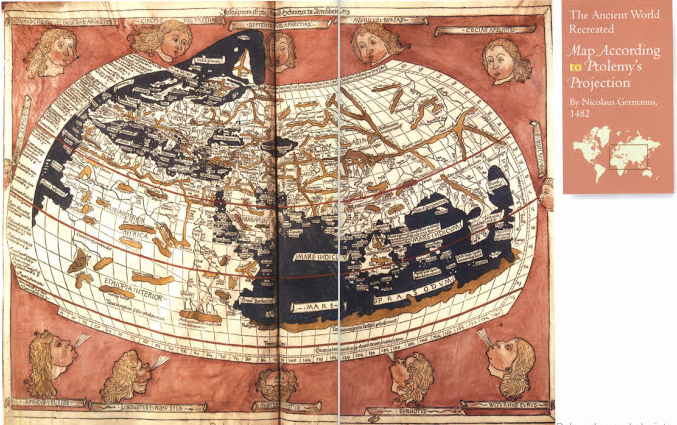
\includegraphics[width=1\textwidth]{figures/PetaPtolemy.PNG}}
	\caption{Gambar Peta menurut Ptolemy}
	\label{PetaPtolemy}
	\end{figure}
	Gambar \ref {PetaPtolemy} Berikut adalah gambar dari Peta yang dibuat oleh Claudius Ptolemy.
	Claudius Ptolemaues yang dikenal dengan nama Ptolemy, hidup antara tahun 100 M dan 168 M, beliau merupakan salah satu sarjana sains pada masanya. Dia tinggal dan bekerja di Alexandria, kota Mesir yang merupakan pusat Intelektual dunia barat dengan perpustakaan paling luas yang pernah diciptakan. Ptolemy membawa semua pengetahuan dan keterampilan matematika dan astronomi dan menerapkannya pada pembuatan peta. Dia memiliki daya tarik matematikawan dengan presisi untuk menunjukkan hubungan satu tempat ke tenpat lain. Berdasarkan perhitungan lingkaran dunia 18.000 mil, ia juga mengembangkan sistem grid latude dan longtude yang dirancang oleh Marinus of Tire. sementara beberapa rincian peta mungkin sedikit aneh dengan garis lintang sejajar dengan garis khatulistiwa dengan garis bujur yang membentang ke utara-selatan dengan busur anggun, sudah tidak asing lagi bagi siapa saja yang pernah memiliki atlas. dalam kerangka ini, ptolemy mampu membangun koordinat dan mendaftarkan lebih dari 8000 tempat dengan koordinat masing-masing. Bagi ptolemy, ini adalah latihan matematik dan kita tidak akan pernah tahu apakah dia benar-benar menggambar peta dari sini.
	Data-data tentang Pembuatan peta sempat hilang ketika perpustakaan Alexandria yang terkenal dibakar oleh orang-orang kristen fanatik pada tahun 390 Masehi - sebuah contoh awal konflik antara iman dan sains. Tapi setidaknya satu salinan yang tealah dibuat dari karya Ptolemy terselamatkan dan ini bertahan di Byzantium. 1000 tahun berlalu dan kemudian tulisannya digunakan untuk dikembangkan oleh ilmuwan Arab, sementara di bagian eropa tetap dalam ketidaktahuan akan warisannya. Baru pada saat renaisans muncul di italia dan daya tarik di dunia, Geografi Ptolemy diterjemahkan dalam bahasa Latin dan gagasannya terhadap PETA Duniadapat diakses oleh para ilmuwan.
	Namun tidak ada peta dalam keadaan masih utuh, hanya petunjuk dan saran untuk pembuatan map dan daftar koordinat.\cite{smart2005maps}
	\begin{figure} [ht]
	\centerline{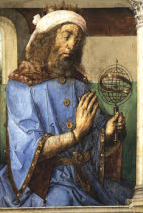
\includegraphics[width=1\textwidth]{figures/ptolemy.PNG}}
	\caption{Foto Ptolemy}
	\label{PetaPtolemy}
	\end{figure}
	gambar \ref{ptolemy} Foto Ptolemy seorang ahli astronomi, geografi, matematikawan.

\subsection{Peta Dunia Ptolemy}
		Peta dunia Ptolemy adalah peta gambaran dunia yang diketahui masyarakat barat pada kurun kedua masihi.Peta tersebut berdasarkan penerangan yang terkandung didalam buku Geographia, ditulis kira-kira pada 150 masihi. walaupun peta autentik tidak dijumpai, buku Geographia yng mengandungi beribu-ribu rujukan pelbagai tempat di dunia lama, berserta kordinat, yang membolehkan para pelukis peta menyusun semula peta dunia Ptolemy apabila manuskriptnya telah ditemui sekitar 1300 masihi.
	\begin{figure} [ht]
	\centerline{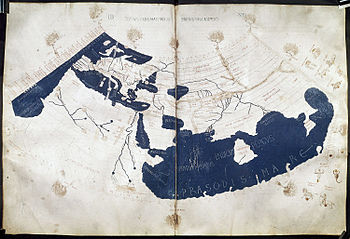
\includegraphics[width=1\textwidth]{figures/PtolemyWorldMap.PNG}}
	\caption{Gambar Ptolemy}	
	\label{PtolemyWorldMap}
	\end{figure}	
	gambar \ref{PetaPtolemy} Peta Dunia Ptolemy, disusun semula dari Geographia Ptolemy (kira-kira 150) pada kurun ke 15, menunjukan ``Sinae" (China) di sebelah kanan, dibawah pulau ``Taprobane" (Sri Lanka, diperbesarkan) dan ``Aurea Chersonesus" (Semenanjung Asia Tenggara).
	\begin{figure} [ht]
	\centerline{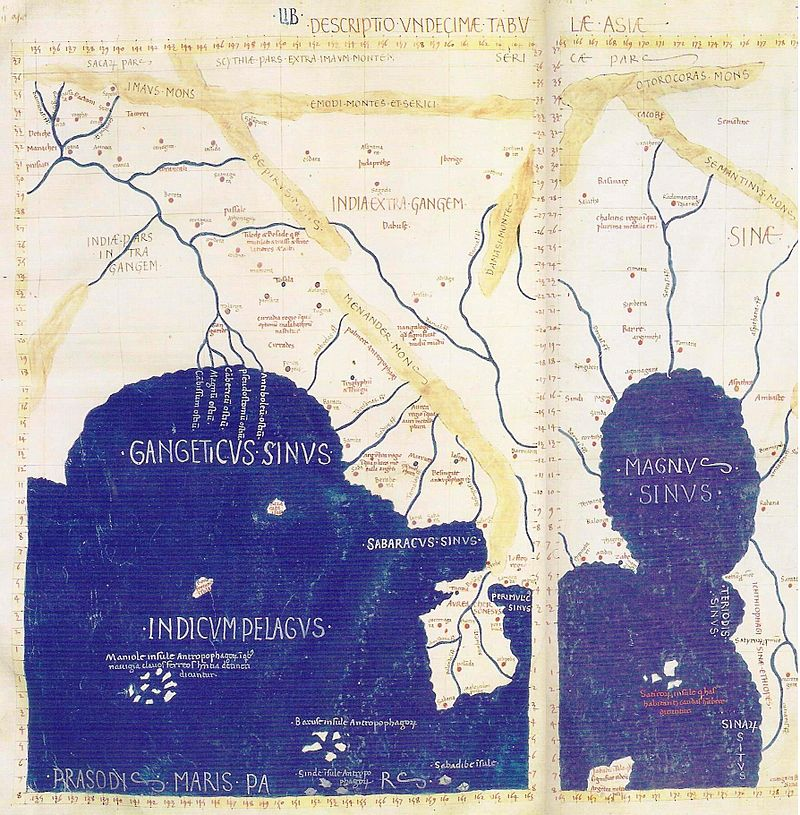
\includegraphics[width=1\textwidth]{figures/PtolemyAsiadetail.PNG}}	
	\caption{Gambar Perincian Timur dan Asia}		
	\end{figure}
	gambar \ref{PtolemyAsiadetail} Perinician Timur dan Asia Tenggara dalam peta dunia Ptolemy.Teluk Ganges (Teluk Bengali) kiri, Semenanjung Asia Tenggara di tengah, Laut China selatan kanan, bersama ``Sinae" (China).
	\subsection{Sejarah ``Ptolemy"}
	\begin{figure} [ht]
	\centerline{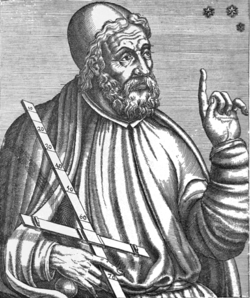
\includegraphics[width=1\textwidth]{figures/Ptolemyporg.PNG}}
	\caption{Konsep artis zaman pertengahan dari Claudius Ptolemaeus.}
	\end{figure}
    gambar \ref{Ptolemyporg}Claudius Ptolemaeus (bahasa Yunani: Κλαύδιος Πτολεμαῖος; 90 – 168), adalah seorang ahli geografi, astronom, dan astrolog yang hidup pada zaman Helenistik di provinsi Romawi, Aegyptus.
    Ptolemaeus adalah pengarang beberapa risalah ilmiah, tiga di antaranya kemudian memainkan peranan penting dalam keilmuwan Islam dan Eropa. Yang pertama adalah risalah astronomi yang dikenal sebagai Almagest (dalam bahasa Yunani Η μεγάλη Σύνταξις , ``Risalah Besar"). Yang kedua adalah Geographia, yang merupakan diskusi teliti mengenai pengetahuan geografi Helenistik. Yang ketiga adalah risalah astrologi dikenal sebagai Tetrabiblos (``Empat buku") di mana dia berusaha mengadaptasi astrologi horoskop ke filosofi alam Aristotelian. Ia juga melestarikan daftar raja-raja kuno, disebut ``Kanon Ptolemaeus", yang penting bagi penelitian sejarah Timur Tengah.
    Claudius adalah nomen (nama keluarga) seorang Roma; Ptolemaeus menyandang nama itu, sehingga menjadi bukti bahwa dia adalah seorang warganegara Roma. Sesuai kebiasaan, Keluarga Ptolemy pertama yang menjadi warganegara (entah itu dia atau nenek moyangnya) mengambil nama itu dari seorang Roma yang bernama Claudius, sehingga membuatnya diberi status kewarganegaraan. Jika orang Roma ini adalah kaisar, kewarganegaraan sudah akan diberi di antara tahun 41 dan 68 M. (waktu Claudius, lalu Nero, menjabat kaisar). Astronom itu juga mempunyai praenomen (nama pertama), yang tetap tak diketahui. Tetapi, kemungkinan Tiberius, karena praenomen itu sangat umum di antara yang keluarga-keluarga yang diberi kewarganegaraan oleh kaisar ini.
    Ptolemaeus (Ptolemy) adalah sebuah nama Yunani. Muncul satu kali di mitologi Yunani, dalam bentuk Homeric. Cukup biasa di antara golongan sol bagian atas Makedonia pada saat Alexander Agung, dan ada beberapa di antara tentara Alexander, satu di antaranya pada tahun 323 S.M. menjadikan dirinya sendiri Raja Mesir: Ptolemy I Soter; semua raja setelah dia, sampai Mesir menjadi provinsi Roma pada tahun 30 S.M., adalah juga dari dinasti Ptolemaic. Hanya ada sedikit bukti tentang subyek asal usul Ptolemy (meskipun melihat di atas kewarganegaraan Roma keluarganya), tetapi kebanyakan sarjana dan sejarawan mempertimbangkannya tak mungkin bahwa Ptolemeus berhubungan dengan dinasti kerajaan Ptolemies.
    Selain dianggap sebagai seorang anggota masyarakat Yunani Alexandria, hanya sedikit rincian hidup Ptolemaeus yang diketahui. Dia menulis dalam bahasa Yunani Kuno dan diketahui sudah menggunakan data astronomis Babilonia.Seorang warganegara Roma, beberapa sarjana menyimpulkan bahwa secara etnik, Ptolemeus adalah orang Yunani, dan sarjana lainnya berpendapat bahwa dia secara etnik orang Mesir, meskipun Hellenize. Dia banyak dikenal dalam sumber bahasa Arab yang muncul kemudian sebagai Upper Egyptian, diperkirakan dia mungkin berasal dari Mesir selatan. Astronom, ahli ilmu bumi, dan pakar fisika Arab selanjutnya merujuk padanya menggunakan nama Arabnya Batlamyus.
    Karya utama Ptolemy lainnya adalah Geografinya (juga disebut Geographia), kompilasi koordinat geografis dari bagian dunia yang dikenal oleh Kekaisaran Romawi pada masanya. Dia agak bergantung pada karya seorang ahli geografi sebelumnya, Marinos of Tire, dan pada kano Romawi dan Kekaisaran Persia kuno. [Rujukan?] Dia juga mengakui astronom Hipparchus kuno karena telah menyediakan ketinggian kutub utara untuk beberapa kota. [19]
   
\subsection{The Geography}	
   \begin{figure} [ht]
	\centerline{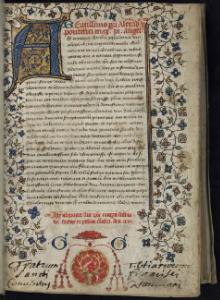
\includegraphics[width=1\textwidth]{figures/geography.PNG}}
	\caption{Geography by Ptolemy.}
		\end{figure}
    gambar \ref{geography} Bagian pertama dari Geografi adalah diskusi tentang data dan metode yang dia gunakan. Seperti model tata surya di Almagest, Ptolemy memasukkan semua informasi ini ke dalam skema besar. Setelah Marinos, dia memberikan koordinat ke semua tempat dan fitur geografis yang dia ketahui, dalam kotak yang membentang di seluruh dunia. Lintang diukur dari khatulistiwa, seperti sekarang, tapi Ptolemy lebih suka [20] untuk mengekspresikannya sebagai climata, panjang hari terpanjang daripada deretan busur: panjang hari senin mulai meningkat dari 12h menjadi 24 jam saat seseorang pergi. dari khatulistiwa ke lingkaran kutub. Dalam buku 2 sampai 7, dia menggunakan gelar dan meletakkan garis meridian 0 bujur di tanah paling barat yang dia kenal, ``Kepulauan Terberkati", yang sering diidentifikasi sebagai Kepulauan Canary, seperti yang disarankan oleh lokasi dari enam titik yang diberi label ``FORTUNATA" pulau-pulau di dekat ekstrem kiri laut biru peta Ptolemeus di sini direproduksi.
	Ptolemeus juga merancang dan memberikan petunjuk bagaimana membuat peta di seluruh dunia yang berpenghuni (oikoumenè) dan provinsi Romawi. Di bagian kedua Geografi, dia memberikan daftar topografi yang diperlukan, dan teks untuk peta. Oikoumenènya membentang 180 derajat bujur dari Kepulauan Terberkati di Samudra Atlantik sampai ke Cina tengah, dan sekitar 80 derajat garis lintang dari Shetland menjadi anti-Meroe (pantai timur Afrika); Ptolemy sangat sadar bahwa dia tahu tentang hanya seperempat dunia, dan perpanjangan yang salah dari Cina ke selatan menunjukkan sumbernya tidak sampai ke Samudra Pasifik.
	Peta di manuskrip yang masih ada di Ptolemy's Geography, bagaimanapun, hanya berasal dari sekitar tahun 1300, setelah teks tersebut ditemukan kembali oleh Maximus Planudes. Tampaknya tabel topografi dalam buku 2-7 adalah teks kumulatif - teks yang diubah dan ditambahkan sebagai pengetahuan baru yang tersedia di abad setelah Ptolemy. [21] Ini berarti bahwa informasi yang terdapat di berbagai bagian Geografi kemungkinan berasal dari tanggal yang berbeda. 
	Peta berdasarkan prinsip ilmiah telah dibuat sejak zaman Eratosthenes, pada abad ke-3 SM, namun Ptolemy memperbaiki proyeksi peta. Diketahui dari sebuah pidato oleh Eumenius bahwa peta dunia, sebuah orbis pictus, yang tidak diragukan lagi berdasarkan Geografi, dipajang di sebuah sekolah di Augustodunum, Gaul pada abad ketiga. [22] Pada abad ke-15, Geografi Ptolemy mulai dicetak dengan peta terukir; edisi cetak paling awal dengan peta terukir diproduksi di Bologna pada 1477, diikuti dengan cepat oleh edisi Romawi tahun 1478 (Campbell, 1987). Sebuah edisi yang dicetak di Ulm pada tahun 1482, termasuk peta tebing kayu, adalah yang pertama dicetak di utara Pegunungan Alpen. Peta terlihat terdistorsi bila dibandingkan dengan peta modern, karena data Ptolemy tidak akurat. Salah satu alasannya adalah Ptolemy memperkirakan ukuran Bumi terlalu kecil: sementara Eratosthenes menemukan 700 stadion untuk sebuah lingkaran besar di dunia, Ptolemy menggunakan 500 stadion di Geografi. Sangat mungkin bahwa ini adalah stadion yang sama, karena Ptolemy beralih dari skala sebelumnya ke yang terakhir antara Syntaxis dan Geography, dan menyesuaikan derajat bujur yang sesuai. Lihat juga unit pengukuran dan Sejarah Yunani Kuno geodesi.
	Karena Ptolemy berasal dari garis lintang utamanya dari nilai terpanjang minyak mentah, garis lintangnya rata-rata keliru kira-kira satu derajat (2 derajat untuk Bizantium, 4 derajat untuk Kartago), meskipun para astronom kuno mampu mengetahui garis lintang mereka lebih lama. (Lambang Ptolemeus sendiri salah oleh 14 '.) Dia setuju (Geografi 1.4) bahwa bujur paling baik ditentukan oleh observasi simultan gerhana bulan, namun dia sangat tidak berhubungan dengan ilmuwan pada masanya bahwa dia tidak mengetahui data semacam itu. lebih baru dari 500 tahun sebelumnya (Arbela gerhana). Ketika beralih dari 700 stadia per derajat ke 500, dia (atau Marinos) memperluas perbedaan bujur antara kota-kota yang sesuai (sebuah titik yang pertama kali direalisasikan oleh P.Gosselin pada tahun 1790), yang mengakibatkan peregangan skala bumi timur-barat yang serius dalam derajat, meski tidak jauh. Mencapai garis bujur yang sangat tepat tetap menjadi masalah dalam geografi sampai penerapan metode bulan Jovian Galileo di abad ke-18. Harus ditambahkan bahwa daftar topografinya yang asli tidak dapat direkonstruksi: tabel panjang dengan angka dikirim ke anak cucu melalui salinan yang mengandung banyak kesalahan juru tulis, dan orang selalu menambahkan atau memperbaiki data topografi: ini adalah kesaksian akan popularitas yang terus-menerus dari Karya ini berpengaruh dalam sejarah kartografi.
	}
=======
%kelompok 2 GIS (Ptolemy)
%Tiara Rizki Wulansari (1154026)
% Muhamad Rifan Zamaludin (1154088)
% Mohammad Agung Deomartha (1154032)
% M. Fajri Mualim (1154078)
% Faisal Syarifuddin

\section{Peta}
	peta adalah/merupakan penggambaran secara grafis atau bentuk skala (perbandingan) pada konsep mengenai bumi. dalam hal ini peta merupakan alat untuk menyampaikan atau menginformasikan mengenai ilmu kebumian. bagaimana peta dahulu ditemukan ? pengetahuan mengenai dasar pembentukan peta sama seperti filosofi, yang mana sering terdapat perbedaan.

\subsection{Peta Menurut Claudius Ptolemaeus Ptolemy}
	\begin{figure} [ht]
	\centerline{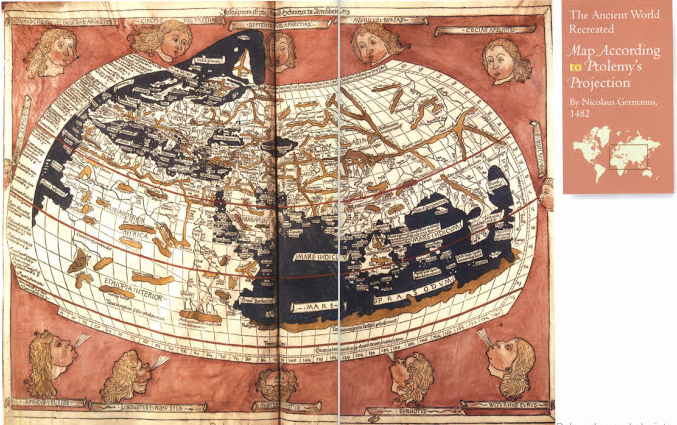
\includegraphics[width=1\textwidth]{figures/PetaPtolemy.PNG}}
	\caption{Gambar Peta menurut Ptolemy}
	\label{PetaPtolemy}
	\end{figure}
	Gambar \ref {PetaPtolemy} Berikut adalah gambar dari Peta yang dibuat oleh Claudius Ptolemy.
	Claudius Ptolemaues yang dikenal dengan nama Ptolemy, hidup antara tahun 100 M dan 168 M, beliau merupakan salah satu sarjana sains pada masanya. Dia tinggal dan bekerja di Alexandria, kota Mesir yang merupakan pusat Intelektual dunia barat dengan perpustakaan paling luas yang pernah diciptakan. Ptolemy membawa semua pengetahuan dan keterampilan matematika dan astronomi dan menerapkannya pada pembuatan peta. Dia memiliki daya tarik matematikawan dengan presisi untuk menunjukkan hubungan satu tempat ke tenpat lain. Berdasarkan perhitungan lingkaran dunia 18.000 mil, ia juga mengembangkan sistem grid latude dan longtude yang dirancang oleh Marinus of Tire. sementara beberapa rincian peta mungkin sedikit aneh dengan garis lintang sejajar dengan garis khatulistiwa dengan garis bujur yang membentang ke utara-selatan dengan busur anggun, sudah tidak asing lagi bagi siapa saja yang pernah memiliki atlas. dalam kerangka ini, ptolemy mampu membangun koordinat dan mendaftarkan lebih dari 8000 tempat dengan koordinat masing-masing. Bagi ptolemy, ini adalah latihan matematik dan kita tidak akan pernah tahu apakah dia benar-benar menggambar peta dari sini.
	Data-data tentang Pembuatan peta sempat hilang ketika perpustakaan Alexandria yang terkenal dibakar oleh orang-orang kristen fanatik pada tahun 390 Masehi - sebuah contoh awal konflik antara iman dan sains. Tapi setidaknya satu salinan yang tealah dibuat dari karya Ptolemy terselamatkan dan ini bertahan di Byzantium. 1000 tahun berlalu dan kemudian tulisannya digunakan untuk dikembangkan oleh ilmuwan Arab, sementara di bagian eropa tetap dalam ketidaktahuan akan warisannya. Baru pada saat renaisans muncul di italia dan daya tarik di dunia, Geografi Ptolemy diterjemahkan dalam bahasa Latin dan gagasannya terhadap PETA Duniadapat diakses oleh para ilmuwan.
	Namun tidak ada peta dalam keadaan masih utuh, hanya petunjuk dan saran untuk pembuatan map dan daftar koordinat \cite{smart2005maps}.
	\begin{figure} [ht]
	\centerline{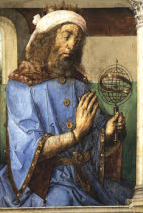
\includegraphics[width=1\textwidth]{figures/ptolemy.PNG}}
	\caption{Foto Ptolemy}
	\label{ptolemy}
	\end{figure}
	gambar \ref{ptolemy} Foto Ptolemy seorang ahli astronomi, geografi, matematikawan.

\subsection{Peta Dunia Ptolemy}
		Peta dunia Ptolemy adalah peta gambaran dunia yang diketahui masyarakat barat pada kurun kedua masihi.Peta tersebut berdasarkan penerangan yang terkandung didalam buku Geographia, ditulis kira-kira pada 150 masihi. walaupun peta autentik tidak dijumpai, buku Geographia yng mengandungi beribu-ribu rujukan pelbagai tempat di dunia lama, berserta kordinat, yang membolehkan para pelukis peta menyusun semula peta dunia Ptolemy apabila manuskriptnya telah ditemui sekitar 1300 masihi.
	\begin{figure} [ht]
	\centerline{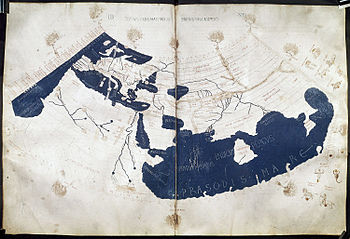
\includegraphics[width=1\textwidth]{figures/PtolemyWorldMap.PNG}}
	\caption{Gambar Ptolemy}	
	\label{PtolemyWorldMap}
	\end{figure}
	gambar \ref {PtolemyWorldMap} Peta Dunia Ptolemy, disusun semula dari Geographia Ptolemy (kira-kira 150) pada kurun ke 15, menunjukan Sinae (China) di sebelah kanan, dibawah pulau Taprobane (Sri Lanka, diperbesarkan) dan Aurea Chersonesus (Semenanjung Asia Tenggara).

	\begin{figure} [ht]
	\centerline{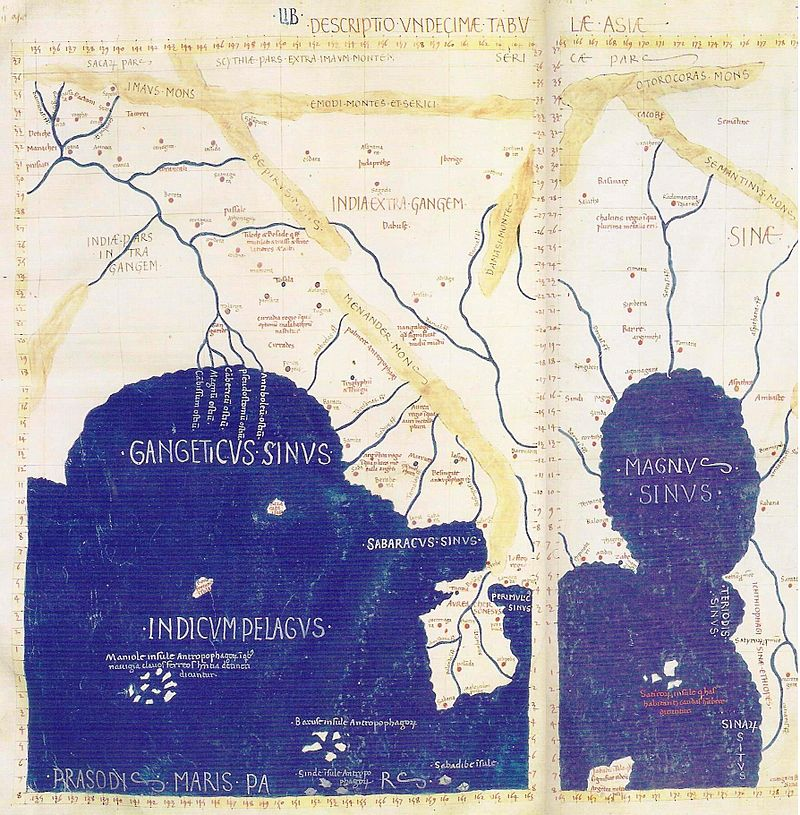
\includegraphics[width=1\textwidth]{figures/PtolemyAsiadetail.PNG}}	
	\caption{Gambar Perincian Timur dan Asia}
	\label{PtolemyAsiadetail}		
	\end{figure}
	gambar \ref{PtolemyAsiadetail} Perinician Timur dan Asia Tenggara dalam peta dunia Ptolemy.Teluk Ganges (Teluk Bengali) kiri, Semenanjung Asia Tenggara di tengah, Laut China selatan kanan, bersama Sinae (China).
	
\subsection{Sejarah Ptolemy}
	\begin{figure} [ht]
	\centerline{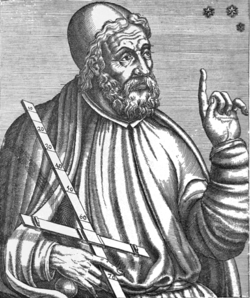
\includegraphics[width=1\textwidth]{figures/Ptolemyporg.PNG}}
	\caption{Konsep artis zaman pertengahan dari Claudius Ptolemaeus.}
	\label{Ptolemyporg}
	\end{figure}
    gambar \ref{Ptolemyporg} Claudius Ptolemaeus (bahasa Yunani: Κλαύδιος Πτολεμαῖος; 90 – 168), adalah seorang ahli geografi, astronom, dan astrolog yang hidup pada zaman Helenistik di provinsi Romawi, Aegyptus.
    Ptolemaeus adalah pengarang beberapa risalah ilmiah, tiga di antaranya kemudian memainkan peranan penting dalam keilmuwan Islam dan Eropa. Yang pertama adalah risalah astronomi yang dikenal sebagai Almagest (dalam bahasa Yunani Η μεγάλη Σύνταξις , Risalah Besar). Yang kedua adalah Geographia, yang merupakan diskusi teliti mengenai pengetahuan geografi Helenistik. Yang ketiga adalah risalah astrologi dikenal sebagai Tetrabiblos (Empat buku) di mana dia berusaha mengadaptasi astrologi horoskop ke filosofi alam Aristotelian. Ia juga melestarikan daftar raja-raja kuno, disebut Kanon Ptolemaeus, yang penting bagi penelitian sejarah Timur Tengah.
    Claudius adalah nomen (nama keluarga) seorang Roma; Ptolemaeus menyandang nama itu, sehingga menjadi bukti bahwa dia adalah seorang warganegara Roma. Sesuai kebiasaan, Keluarga Ptolemy pertama yang menjadi warganegara (entah itu dia atau nenek moyangnya) mengambil nama itu dari seorang Roma yang bernama Claudius, sehingga membuatnya diberi status kewarganegaraan. Jika orang Roma ini adalah kaisar, kewarganegaraan sudah akan diberi di antara tahun 41 dan 68 M. (waktu Claudius, lalu Nero, menjabat kaisar). Astronom itu juga mempunyai praenomen (nama pertama), yang tetap tak diketahui. Tetapi, kemungkinan Tiberius, karena praenomen itu sangat umum di antara yang keluarga-keluarga yang diberi kewarganegaraan oleh kaisar ini.
    Ptolemaeus (Ptolemy) adalah sebuah nama Yunani. Muncul satu kali di mitologi Yunani, dalam bentuk Homeric. Cukup biasa di antara golongan sol bagian atas Makedonia pada saat Alexander Agung, dan ada beberapa di antara tentara Alexander, satu di antaranya pada tahun 323 S.M. menjadikan dirinya sendiri Raja Mesir: Ptolemy I Soter; semua raja setelah dia, sampai Mesir menjadi provinsi Roma pada tahun 30 S.M., adalah juga dari dinasti Ptolemaic. Hanya ada sedikit bukti tentang subyek asal usul Ptolemy (meskipun melihat di atas kewarganegaraan Roma keluarganya), tetapi kebanyakan sarjana dan sejarawan mempertimbangkannya tak mungkin bahwa Ptolemeus berhubungan dengan dinasti kerajaan Ptolemies.
    Selain dianggap sebagai seorang anggota masyarakat Yunani Alexandria, hanya sedikit rincian hidup Ptolemaeus yang diketahui. Dia menulis dalam bahasa Yunani Kuno dan diketahui sudah menggunakan data astronomis Babilonia.Seorang warganegara Roma, beberapa sarjana menyimpulkan bahwa secara etnik, Ptolemeus adalah orang Yunani, dan sarjana lainnya berpendapat bahwa dia secara etnik orang Mesir, meskipun Hellenize. Dia banyak dikenal dalam sumber bahasa Arab yang muncul kemudian sebagai Upper Egyptian, diperkirakan dia mungkin berasal dari Mesir selatan. Astronom, ahli ilmu bumi, dan pakar fisika Arab selanjutnya merujuk padanya menggunakan nama Arabnya Batlamyus.
    Karya utama Ptolemy lainnya adalah Geografinya (juga disebut Geographia), kompilasi koordinat geografis dari bagian dunia yang dikenal oleh Kekaisaran Romawi pada masanya. Dia agak bergantung pada karya seorang ahli geografi sebelumnya, Marinos of Tire, dan pada kano Romawi dan Kekaisaran Persia kuno. [Rujukan] Dia juga mengakui astronom Hipparchus kuno karena telah menyediakan ketinggian kutub utara untuk beberapa kota.[19]
  
  \subsection{The Geography}	
   \begin{figure} [ht]
	\centerline{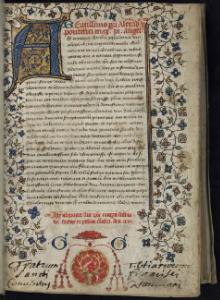
\includegraphics[width=1\textwidth]{figures/geography.PNG}}
	\caption{Geography by Ptolemy.}
	\label{geography}
		\end{figure}
    gambar \ref {geography} Bagian pertama dari Geografi adalah diskusi tentang data dan metode yang dia gunakan. Seperti model tata surya di Almagest, Ptolemy memasukkan semua informasi ini ke dalam skema besar. Setelah Marinos, dia memberikan koordinat ke semua tempat dan fitur geografis yang dia ketahui, dalam kotak yang membentang di seluruh dunia. Lintang diukur dari khatulistiwa, seperti sekarang, tapi Ptolemy lebih suka [20] untuk mengekspresikannya sebagai climata, panjang hari terpanjang daripada deretan busur: panjang hari senin mulai meningkat dari 12h menjadi 24 jam saat seseorang pergi. dari khatulistiwa ke lingkaran kutub. Dalam buku 2 sampai 7, dia menggunakan gelar dan meletakkan garis meridian 0 bujur di tanah paling barat yang dia kenal, Kepulauan Terberkati, yang sering diidentifikasi sebagai Kepulauan Canary, seperti yang disarankan oleh lokasi dari enam titik yang diberi label FORTUNATA pulau-pulau di dekat ekstrem kiri laut biru peta Ptolemeus di sini direproduksi.
	Ptolemeus juga merancang dan memberikan petunjuk bagaimana membuat peta di seluruh dunia yang berpenghuni (oikoumenè) dan provinsi Romawi. Di bagian kedua Geografi, dia memberikan daftar topografi yang diperlukan, dan teks untuk peta. Oikoumenènya membentang 180 derajat bujur dari Kepulauan Terberkati di Samudra Atlantik sampai ke Cina tengah, dan sekitar 80 derajat garis lintang dari Shetland menjadi anti-Meroe (pantai timur Afrika); Ptolemy sangat sadar bahwa dia tahu tentang hanya seperempat dunia, dan perpanjangan yang salah dari Cina ke selatan menunjukkan sumbernya tidak sampai ke Samudra Pasifik.
	Peta di manuskrip yang masih ada di Ptolemy's Geography, bagaimanapun, hanya berasal dari sekitar tahun 1300, setelah teks tersebut ditemukan kembali oleh Maximus Planudes. Tampaknya tabel topografi dalam buku 2-7 adalah teks kumulatif - teks yang diubah dan ditambahkan sebagai pengetahuan baru yang tersedia di abad setelah Ptolemy. [21] Ini berarti bahwa informasi yang terdapat di berbagai bagian Geografi kemungkinan berasal dari tanggal yang berbeda. 
	Peta berdasarkan prinsip ilmiah telah dibuat sejak zaman Eratosthenes, pada abad ke-3 SM, namun Ptolemy memperbaiki proyeksi peta. Diketahui dari sebuah pidato oleh Eumenius bahwa peta dunia, sebuah orbis pictus, yang tidak diragukan lagi berdasarkan Geografi, dipajang di sebuah sekolah di Augustodunum, Gaul pada abad ketiga. [22] Pada abad ke-15, Geografi Ptolemy mulai dicetak dengan peta terukir; edisi cetak paling awal dengan peta terukir diproduksi di Bologna pada 1477, diikuti dengan cepat oleh edisi Romawi tahun 1478 (Campbell, 1987). Sebuah edisi yang dicetak di Ulm pada tahun 1482, termasuk peta tebing kayu, adalah yang pertama dicetak di utara Pegunungan Alpen. Peta terlihat terdistorsi bila dibandingkan dengan peta modern, karena data Ptolemy tidak akurat. Salah satu alasannya adalah Ptolemy memperkirakan ukuran Bumi terlalu kecil: sementara Eratosthenes menemukan 700 stadion untuk sebuah lingkaran besar di dunia, Ptolemy menggunakan 500 stadion di Geografi. Sangat mungkin bahwa ini adalah stadion yang sama, karena Ptolemy beralih dari skala sebelumnya ke yang terakhir antara Syntaxis dan Geography, dan menyesuaikan derajat bujur yang sesuai. Lihat juga unit pengukuran dan Sejarah Yunani Kuno geodesi.
	Karena Ptolemy berasal dari garis lintang utamanya dari nilai terpanjang minyak mentah, garis lintangnya rata-rata keliru kira-kira satu derajat (2 derajat untuk Bizantium, 4 derajat untuk Kartago), meskipun para astronom kuno mampu mengetahui garis lintang mereka lebih lama. (Lambang Ptolemeus sendiri salah oleh 14.) Dia setuju (Geografi 1.4) bahwa bujur paling baik ditentukan oleh observasi simultan gerhana bulan, namun dia sangat tidak berhubungan dengan ilmuwan pada masanya bahwa dia tidak mengetahui data semacam itu. lebih baru dari 500 tahun sebelumnya (Arbela gerhana). Ketika beralih dari 700 stadia per derajat ke 500, dia (atau Marinos) memperluas perbedaan bujur antara kota-kota yang sesuai (sebuah titik yang pertama kali direalisasikan oleh P.Gosselin pada tahun 1790), yang mengakibatkan peregangan skala bumi timur-barat yang serius dalam derajat, meski tidak jauh. Mencapai garis bujur yang sangat tepat tetap menjadi masalah dalam geografi sampai penerapan metode bulan Jovian Galileo di abad ke-18. Harus ditambahkan bahwa daftar topografinya yang asli tidak dapat direkonstruksi: tabel panjang dengan angka dikirim ke anak cucu melalui salinan yang mengandung banyak kesalahan juru tulis, dan orang selalu menambahkan atau memperbaiki data topografi: ini adalah kesaksian akan popularitas yang terus-menerus dari Karya ini berpengaruh dalam sejarah kartografi.
	
>>>>>>> 6a8108a428c212f725996110cef23fc85d44868e


%\chapter[Sejarah eratosthenes]
%{Pendahuluan\\ eratosthenes}
%% kelompok Eratosthenes
% Boby Jamis Hari Sel (1154040)
% Diki Wahyu Nugraha (1154059)
% Restiyana Dwi Astuti (1154077)
% Rizky Abdi Perdana (1154007)
% Sabda Alamsyah (1154111)

\section{Eratosthenes}
Lebih dari 2000 tahun yang lalu Eratosthenes membandingkan posisi Matahari di dua lokasi untuk menentukan ukuran bumi dengan alasan yang akurat.
Berdasarkan \cite{plochmann1983dictionary} Eratosthenes lahir di Yunani pada koloni yang bernama Cyrene, sekarang disebut kota Shahhat, Libya, Sebagai pemuda, dia  pergi ke athena demi melanjutkan studinya. Lalu ua kembali ke Cyrene, dan membuat nama untuk dirinya sendiri untuk kebutuhan ilmiah sehingga penguasa Yunani di Mesir membawanya ke Aleksandria.
Seorang pria yang mempunyai banyak talenta, Eratosthenes adalah seorang pustakawan, geografer, matematikawan, astronom, sejarahwan dan penyair. Teman-temannya di perpustakaan menjulukinya sebagai Pentathlos atau atlit yang berkompetisi dalam lima acara yang berbeda. Julukan itu seperinya cocok ditujukan kepada untuk seorang penerima beasiswa dari banyak bidang studi. Banyak dari tulisan karya Eratosthenes telah hilang tetapi ada beberapa orang yang melaporkan pekerjaannya telah ditemukan. \cite{lasky2008librarian}
\begin{figure}[ht]
	\centerline{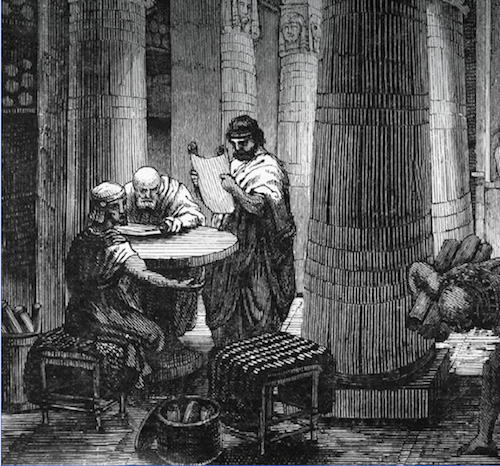
\includegraphics[width=1\textwidth]{figures/illustrasi.jpg}}
	\caption{ilustrasi yang tidak bertanggal dari para ilmuwan di Perpustakaan Alexandria Bettmann / CORBIS}
	\label{illustrasi}
	\end{figure}
\subsection{Bapak Geografi}
Eratosthenes melanjutkan pengetahuannya tentang Bumi. Dengan menggunakan penemuan dan pengetahuan tentang ukuran dan bentuknya, dia mulai membuat sketsa. Di Perpustakaan Alexandria ia memiliki akses ke berbagai buku perjalanan, yang berisi berbagai bentuk informasi dan representasi dunia. \cite{smith2005dictionary} Dalam karya jilid tiga-nya Geografi (bahasa Yunani: Geographika), dia menggambarkan dan memetakan seluruh dunia yang dikenalnya, bahkan membagi Bumi menjadi lima zona iklim: \cite{grimbly2013encyclopedia} dua zona pembekuan di sekitar kutub, dua zona beriklim sedang, dan sebuah zona yang meliputi khatulistiwa dan daerah tropis. Ia telah menemukan geografi. Dia menciptakan terminologi yang masih digunakan sampai sekarang. Dia meletakkan grid garis tumpang tindih di atas permukaan Bumi. Dia menggunakan kesejajaran dan garis meridian untuk menghubungkan setiap tempat di dunia. Sekarang mungkin untuk memperkirakan jarak seseorang dari lokasi dasar jaringan ini di atas permukaan Bumi. Dalam Geografi nama-nama lebih dari 400 kota dan lokasi mereka ditunjukkan:  Sayangnya, Geografi-nya telah hilang dari sejarah, Pliny, Polybius, Strabo, dan Marcianus. \cite{roller2010eratosthenes}
Buku pertama adalah pengantar dan memberikan ulasan tentang pendahulunya, mengakui kontribusi mereka yang dia susun di perpustakaan. Dalam buku ini Eratosthenes mengecam Homer karena tidak memberikan wawasan tentang apa yang sekarang digambarkannya sebagai geografi. Ketidaksetujuannya terhadap topografi Homer membuat marah banyak orang yang percaya bahwa dunia digambarkan dalam Odyssey sebagai hal yang sah. \cite{eckerman2011eratosthenes} Bumi adalah dunia yang tak tergoyahkan; Sementara di permukaannya ada tempat yang sedang berubah. Dia telah berhipotesis bahwa pada suatu waktu Mediterania adalah danau besar yang menutupi negara-negara yang mengelilinginya; dan hanya terhubung ke barat saat sebuah lorong telah dibuka dalam sejarahnya.
Dalam buku kedua adalah penemuannya tentang keliling bumi. Di sinilah, menurut Pliny, ``Dunia digenggam.'' Eratosthenes menggambarkan kisah terkenalnya tentang sumur di Syene, yang dijelaskan di atas. Buku ini akan dianggap sebagai teks tentang geografi matematika.
Buku ketiganya tentang Geografi berisi geografi politik. Dia mengutip negara-negara dan menggunakan garis sejajar untuk membagi peta menjadi beberapa bagian, untuk memberikan deskripsi alam yang akurat. Ini adalah terobosan, dan bisa dianggap sebagai awal geografi. \cite{smith2005dictionary}
\subsection{Mempelajari Bumi}
Eratosthenes mungkin orang pertama yang menggunakan kata geografi. Dia menciptakan sistem garis bujur dan garis lintang dan membuat peta dari dunia yang sekarang dikenal. Dia juga merancang sistem untuk menemukan penomoran utama — bilangan bulat yang hanya dapat dibagi sendiri atau dengan angka 1. Metode ini, masih digunakan sampai hari ini.
Pada saat itu, Eratosthenes mengusulkan sebuah algoritma sederhana untuk menemukan bilangan prima. Algoritma ini dikenal dalam matematika sebagai ``Sieve of Eratosthenes.``
Dalam matematika, Sieve of Eratosthenes, salah satu dari sejumlah saringan bilangan prima, adalah algoritma kuno yang sederhana untuk menemukan semua bilangan prima sampai batas tertentu. Hal itu terjadi karena secara iteratif menandai sebagai komposit, yaitu, tidak prima, kelipatan masing-masing prima, dimulai dengan kelipatan 2. Kelipatan bilangan prima yang diberikan dihasilkan mulai dari yang prima, sebagai urutan angka dengan perbedaan yang sama, sama dengan yang prima, antara angka berurutan. Ini adalah perbedaan kunci saringan dari penggunaan divisi percobaan untuk menguji secara berurutan setiap nomor kandidat untuk dibagi masing-masing prima.
Eeratosthenes juga yang pertama menghitung sumbu kemiringan bumi, yang dia pikir dengan tingkat akurasi yang tinggi; temuan dilaporkan oleh Ptolemy (85-165 M). Eratosthenes juga menghitung jarak dari bumi ke bulan dan ke matahari, tetapi dengan tingkat akurasi yang rendah. Ia membuat katalog 675 bintang. Ia membuat kalender dengan tahun kabisat dan meletakkan dasar chro- nology di dunia barat dengan penyelenggaraan tanggal sastra dan politik kegiatan dari pengepungan Troy (sekitar 1194 - 1184 SM) ke dalam waktu ia sendiri.
Namun, pencapaiannya yang paling abadi adalah perhitungan lingkar bumi yang sangat akurat (jarak di sekitar lingkaran atau bola). Dia menghitung ini dengan menggunakan geometri dan trigonometri sederhana dan dengan mengenali Bumi sebagai bola di ruang angkasa. Sebagian besar ilmuwan Yunani pada masa Aristoteles (384-322 SM) sepakat bahwa Bumi adalah sebuah bola, tapi tidak ada yang tahu seberapa besar itu.
Bagaimana para ilmuwan Yunani mengetahui bahwa bumi adalah sebuah lingkungan? Mereka mengamati bahwa kapal menghilang di atas cakrawala sementara tiang-tiang mereka masih terlihat. Mereka melihat bayangan melengkung Bumi di Bulan selama gerhana bulan. Dan mereka melihat perubahan posisi bintang di langit.
\begin{figure}[ht]
	\centerline{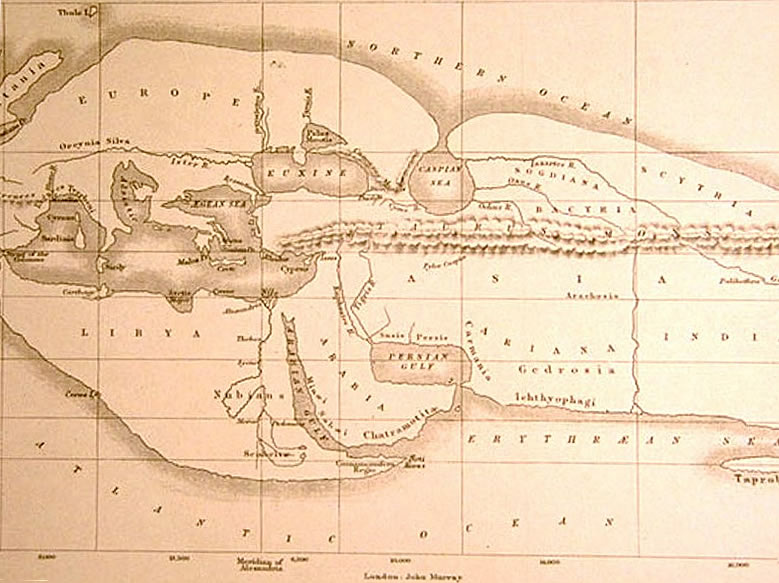
\includegraphics[width=1\textwidth]{figures/194BCEworldmap.jpg}}
	\caption{Rekonstruksi Eratosthenes c. 194 SM peta dunia, dari E.H. Bunbury's 1883 Sejarah Geografi Kuno di antara orang Yunani dan Romawi dari Abad Pertengahan sampai Kejatuhan Kekaisaran Romawi, ranah publik}
	\label{194BCEworldmap}
	\end{figure}
\subsection{Mengukur Bumi}
Eratosthenes mendengar tentang sumur terkenal di kota Swenet Mesir (Syene dalam bahasa Yunani, dan sekarang dikenal sebagai Aswan), di Sungai Nil. Siang hari satu hari setiap tahun - titik balik matahari musim panas (antara 20 Juni dan 22 Juni) - sinar matahari bersinar langsung ke dalam lubang dalam. Mereka hanya menyinari air di bagian bawah, bukan sisi sumur seperti pada hari-hari lain, membuktikan bahwa Matahari langsung di atas kepala. (Syene terletak sangat dekat dengan apa yang kita sebut Tropic of Cancer,  23,5 derajat ke utara, garis lintang paling utara di mana Matahari selalu berada di atas kepala pada siang hari.)
Eratosthenes mendirikan sebuah tiang di Alexandria, dan pada titik balik matahari musim panas ia mengamati bahwa ia melemparkan bayangan, membuktikan bahwa Matahari tidak berada di atas kepala tetapi sedikit ke selatan. Mengakui kelengkungan Bumi dan mengetahui jarak antara kedua kota memungkinkan Eratosthenes untuk menghitung lingkar planet.
\cite{nicastro2008circumference} Eratosthenes bisa mengukur sudut sinar matahari dari vertikal dengan membagi panjang kaki di seberang sudut (panjang bayangan) dengan kaki yang bersebelahan dengan sudut (tinggi tiang). Ini memberinya sudut 7,16 derajat. Dia tahu bahwa lingkar bumi membentuk lingkaran 360 derajat, jadi 7,12 (atau 7,2, untuk membagi 360 secara merata sampai 50) derajatnya kira-kira seper lima puluh keliling. Dia juga tahu perkiraan jarak antara Alexandria dan Syene, jadi dia bisa mengatur persamaan ini:

Eratosthenes memperkirakan jarak dari Alexandria ke Syene sebanyak 5.000 stadion, atau sekitar 500 mil (800 kilometer). Dia membuat estimasi ini dari saat dibutuhkan pejalan kaki, yang dilatih untuk mengukur jarak dengan mengambil langkah reguler, untuk berjalan-jalan di antara kota-kota. Dengan memecahkan persamaan tersebut, dia menghitung keliling 250.000 stadia, atau 25.000 mil (40.000 kilometer) seperti pada gambar \ref{diagrampengukuranbumi}.
\begin{figure}[ht]
	\centerline{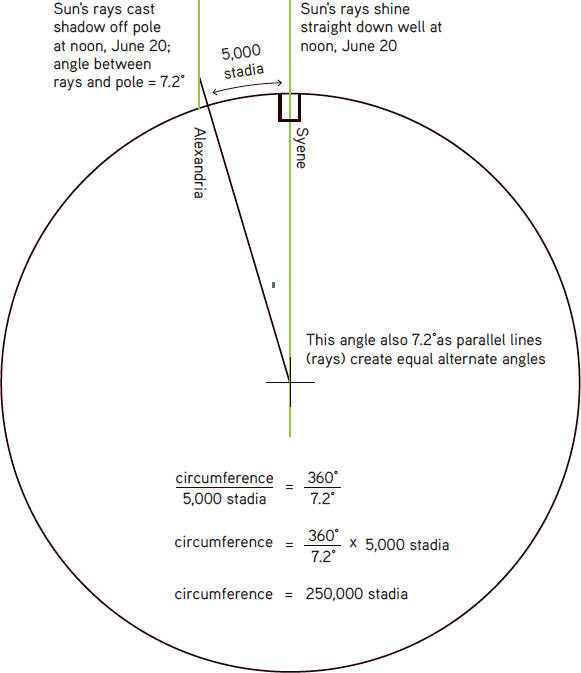
\includegraphics[width=1\textwidth]{figures/diagrampengukuranbumi.png}}
	\caption{Sebuah diagram yang menunjukkan bagaimana Eratosthenes mengukur Bumi, diakses dari Simon Fraser University Online}
	\label{diagrampengukuranbumi}
	\end{figure}
Beberapa sumber kesalahan merembet ke dalam perhitungan Eratosthenes dan interpretasi kita terhadapnya. Untuk satu hal, dia menggunakan unitnya untuk mengukur satuan stadion Yunani atau stadion atletik. Tapi tidak semua stadion dibangun dengan panjang yang sama. Di Yunani sebuah stadion setara dengan 185 meter (607 kaki), sedangkan di Mesir stadion berjarak sekitar 157,5 meter (517 kaki). Kami tidak tahu unit mana yang digunakan Eratosthenes. Jika dia menggunakan ukuran Yunani, perhitungannya akan turun sekitar 16 persen. Jika dia menggunakan orang Mesir, kesalahannya akan berada di bawah 2 persen dari lingkar bumi sebenarnya dari 24.860 mil (40.008 kilometer).
Satu abad setelah Eratosthenes, astronom Yunani Posidonius dari Rhodes (sekitar 135-51 SM) menghitung lingkar bumi. Posidonius menggunakan bintang Canopus sebagai kerangka acuan: ketika bintang tersebut terlihat di cakrawala di Rhodes, itu adalah 7,5 derajat di atas cakrawala di Alexandria. Perhitungan pertamanya hampir benar, tapi dia merevisi jarak antara Rhodes dan Alexandria, yang menghasilkan angka yang sebanding dengan sekitar 18.000 mil (sekitar 29.000 kilometer), sekitar 28 persen lebih kecil dari lingkar sebenarnya. Ptolemy melaporkan perhitungan Posidonius dan bukan kata-kata Eratosthenes, dan tulisan Ptolemy inilah yang menemukan jalan mereka menuju Christopher Columbus. Jika Ptolemy telah menggunakan sosok Eratosthenes yang lebih besar dan lebih akurat untuk keliling bumi, Columbus mungkin tidak akan pernah berlayar ke barat.
Eratosthenes hidup sampai usia 82 tahun, saat dia kelaparan sampai mati karena dia takut pada awitan kebutaan.
\subsection{Prestasi}
Eratosthenes digambarkan oleh Leksikon Suda sebagai $Πένταθλος$ (Pentathlos) yang dapat diterjemahkan sebagai ``All-Rounder'', karena ia ahli dalam berbagai hal: Dia adalah seorang polymath sejati. Dia dijuluki Beta karena dia hebat dalam banyak hal dan mencoba mendapatkan setiap informasi, namun tidak pernah mencapai peringkat tertinggi dalam segala hal; Straboaccounts Eratosthenes sebagai matematikawan di antara ahli geografi dan ahli geografi di kalangan matematikawan.
\begin{itemize}
\item Eusebius dari Kaisarea dalam bukunya Preparatio Evangelica mencakup sebuah bab singkat dari tiga kalimat pada jarak selestial (Kitab XV, Bab 53). Dia menyatakan dengan sederhana bahwa Eratosthenes menemukan jarak ke Matahari untuk menjadi stadion miriad 400 dan 80.000 dan jarak ke Bulan menjadi 780.000 stadion. Ungkapan jarak ke Matahari telah diterjemahkan sebagai 4.080.000 stadia (1903 terjemahan oleh E. H. Gifford), atau sebagai 804.000.000 stadia (edisi Edouard des Places, bertanggal 1974-1991). Artinya tergantung pada apakah Eusebius berarti 400 segudang ditambah 80.000 atau ``400 dan 80.000`` segudang. Dengan stadion 185 m, 804.000.000 stadion adalah 149.000.000 km, kira-kira jaraknya dari Bumi ke Matahari.
\item Menurut \cite{smith2005dictionary} Eratosthenes juga menghitung diameter Matahari. Menurut Macrobious, Eratosthenes membuat diameter Matahari menjadi sekitar 27 kali lipat dari Bumi. Angka sebenarnya kira-kira 109 kali.
\item Selama berada di Perpustakaan Alexandria, Eratosthenes merancang sebuah kalender dengan menggunakan ramalannya tentang ekliptika Bumi. Dia menghitung bahwa ada 365 hari dalam setahun dan setiap tahun keempat akan ada 366 hari.
\item Dia juga sangat bangga dengan solusinya untuk Menggandakan Cube. Motivanya adalah bahwa ia ingin menghasilkan ketapel. Eratosthenes membangun perangkat gambar garis mekanis untuk menghitung kubus, yang disebut mesolabio. Dia mendedikasikan solusinya untuk Raja Ptolemy, menyajikan sebuah model di perunggu dengan sebuah surat dan sebuah epigram. Archimedes adalah teman Eratosthenes dan dia juga mengerjakan alat perang dengan matematika. Archimedes mendedikasikan bukunya The Method to Eratosthenes, mengetahui cintanya untuk belajar dan matematika. \cite{chondros2010archimedes}
\end{itemize}
\subsection{Pekerjaan}
Eratosthenes adalah salah satu tokoh ilmiah paling terkemuka di masanya, dan menghasilkan karya-karya yang mencakup pengetahuan luas sebelum dan selama waktunya di Perpustakaan. Dia menulis banyak topik - geografi, matematika, filsafat, kronologi, kritik sastra, tatabahasa, puisi, dan bahkan komedi lama. Sayangnya, hanya ada sisa fragmen karya-karyanya setelah Penghancuran Perpustakaan Alexandria.

\subsection{Judul karya yang dihasilkan oleh Eratosthenes}
\begin{enumerate}
\item	Platonikos
\item	Hermes
\item	Erigone
\item	Chronographies
\item	On the Measurement of the Earth (hilang)
\item	Geographika (hilang, dikritik oleh Strabo)
\item	Arsinoes (sebuah memoar Ratu Arsinoe; hilang; \cite{gulickathenaeus})
\item	Ariston (tentang Aristo dari Chios kecanduan kemewahan); kalah; dikutip oleh Athenaeus di Deipnosophistae) \cite{gulickathenaeus}
\end{enumerate}



%\chapter[Sejarah aliddrissi]
%{Pendahuluan\\ aliddrissi}
%% Kelompok 3
% Ajrina Dharman (1154079)
% Diana Satima G (1154018)
% Indah Rahmawati (1154070)
% M. Amran Hakim Siregar (1154106)
% Rizky Abdul Ghani Suherli (1154048)

\section{Peta}
	peta adalah/merupakan penggambaran secara grafis atau bentuk skala (perbandingan) pada konsep mengenai bumi. dalam hal ini peta merupakan alat untuk menyampaikan atau menginformasikan mengenai ilmu kebumian. bagaimana peta dahulu ditemukan ? pengetahuan mengenai dasar pembentukan peta sama seperti filosofi, yang mana sering terdapat perbedaan.

\subsection{Peta Menurut Abu Abdullah Muhammad al-Idrisi al-Qurtubi al-Hasani as-Sabti "al-Idrisi"}
	\begin{figure} [ht]
	\centerline{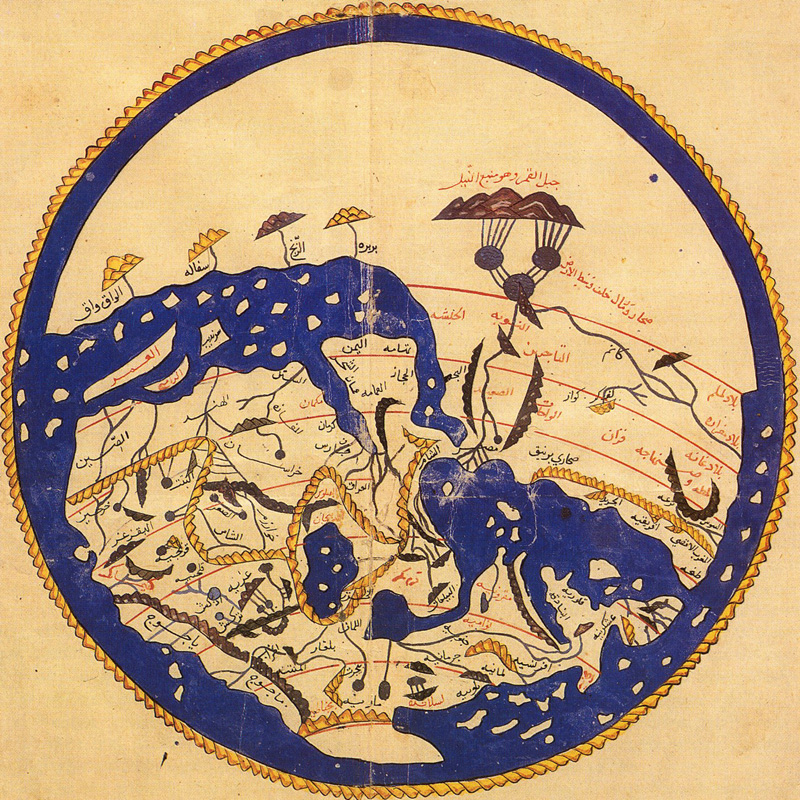
\includegraphics[width=1\textwidth]{figures/1.jpg}}
	\caption{Gambar Peta menurut al-Idrisi}
	\label{Petaal-Idrisi}
	\end{figure}
	\ref{1.jpg} Berikut adalah gambar dari Peta yang dibuat oleh Muhammad al - Idrisi.
	Abu Abdullah Muhammad al-Idrisi al-Qurtubi al-Hasani as-Sabti yang dikenal dengan nama al-Idrisi, hidup antara tahun 1100 – 1165. Al-Idrisi lahir di keluarga Hammudid besar Afrika Utara dan Al-Andalus, yang mengklaim turun dari Idrisids of Morocco dan akhirnya nabi Muhammad. Al-Idrisi lahir di kota Ceuta, di mana kakek buyutnya terpaksa menetap setelah jatuhnya Hammudid Málaga ke Zirids di Granada. Dia menghabiskan sebagian besar masa mudanya untuk bepergian melalui Afrika Utara dan Al-Andalus (Spanyol Muslim saat ini) dan tampaknya telah mendapatkan informasi terperinci mengenai kedua wilayah tersebut. Dia mengunjungi Anatolia saat dia baru berusia 16 tahun. Dia belajar di Córdoba.
	Al-Idrisi memasukkan pengetahuan tentang Afrika, Samudera Hindia dan Timur Jauh yang dikumpulkan oleh pedagang dan penjelajah Islam dan dicatat di peta Islam dengan informasi yang dibawa oleh pelayaran Norman untuk membuat peta dunia yang paling akurat pada zaman pra-modern, yang berfungsi sebagai ilustrasi konkret Kitab nuzhat al-mushtaq-nya, yang dapat diterjemahkan sebagai Pengalihan Manusia untuk Berkelana ke Tempat yang Jauh. 
	Tabula Rogeriana digambar oleh Al-Idrisi pada tahun 1154 untuk Raja Norman Roger II dari Sisilia, setelah tinggal delapan belas tahun di istananya, di mana dia mengerjakan komentar dan ilustrasi peta. Peta tersebut, dengan legenda yang ditulis dalam bahasa Arab, sekaligus menunjukkan benua Eurasia secara keseluruhan, hanya menunjukkan bagian utara benua Afrika dan tidak memiliki rincian Tanduk Afrika dan Asia Tenggara.
	\ref{3.jpg} Berikut adalah gambar dari Peta Tabula Rogeriana digambar oleh Al-Idrisi.
	\begin{figure} [ht]
	\centerline{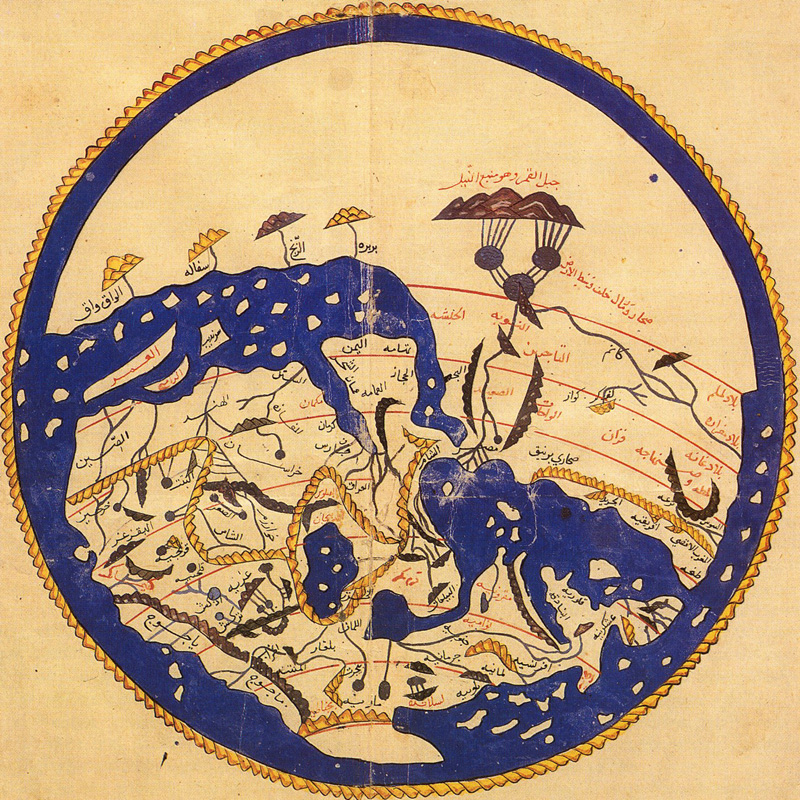
\includegraphics[width=1\textwidth]{figures/1.jpg}}
	\caption{Foto al-Idrisi}
	\end{figure}
	\ref{2.jpg} Foto al-Idrisi seorang ahli geografi,.
	

\subsection {Sejarah Peta dari pandangan Al-Qur'an "al-idrisi"}
	Pandangan Islam mempercayai adanya dua keghaiban, yaitu keghaiban yang eksistensinya tidak harus terukur atau tidak harus difahami melalui metodologi sains, keghaiban yang difahami melalui sistem keimanan, selain itu juga keghaiban yang dikenal sebagai sunattullah. Manusia tak menyaksikan secara langsung tentang proses-proses pembentukan alamsemesta, bahkan kehidupannya di planit Bumi ini hanya merupakan sebagian kecil episode dalam alamsemesta.
	Metodologi sains, Islam memperkenalkan sebuah metodologi lain yaitu ilmupengetahuan (tentang eksistensi kebenaran) bagi manusia bisa bersumber dari sumber terpercaya (kitab Allah) dan disampaikan dengan cara terpercaya. Al Qur’an merupakan sebuah kebenaran yang melengkapi pandangan yang dibangun melalui rasionalitas manusia semata, memperkenalkan Allah sebagai Tuhan alam semesta, ada alam ghaib, ada sesuatu yang ghaib dan manusia tak banyak mengetahuinya, ada cara atau upaya-upaya mencapai atau berkomunikasi dengan Yang MahaPencipta dan MahaPenguasa alam semesta. Pemahaman sunatullah dipergunakan untuk penyempurnaan dan membuat kemudahan-kemudahan dalam hidup dan beribadah agar bisa senantiasa lebih mendekat lagi kepada Allah swt, MahaPencipta dan MahaPenguasa alam semesta.
	Al Qur’an sebagai wahyu Allah yang telah diturunkan kepada umat manusia, perlu dipandang sebagai “resources” bagi kehidupan umat manusia di planit Bumi yaitu sebagai petunjuk Allah swt agar hati manusia bisa tertuntun dan terdidik sehingga berahlak mulia. Gambaran wahyu Allah dalam al Qur'an mengingatkan walaupun ada kepastian dari “tangan-tangan ghaib berupa sunatullah” yang sebagian telah bisa diungkap melalui metodologi sains, namun masih terdapat pengetahuan dan kehendakNya yang ghaib dalam penciptaan Alam Semesta. 
	Pemikiran atas fenomena alam semesta itu sangat diharapkan bisa membangun kesadaran beragama, mempertemukan “kerja tangan-tangan ghaib Allah” yang mengatur alam semesta dengan wahyuNya dalam al Qur’an. Keduanya adalah kebenaran yang berasal dari yang Allah zat yang Maha Esa. Mempertemukan kebenaran wahyu Allah dan ayat kauniyah merupakan proses pemahaman manusia tentang lingkungan kehidupannya yang lebih luas, menjangkau dunia dan akherat, memadukan akal dan keyakinan dalam perspektif Islam. 
	Abad sains dan teknologi telah dijalani manusia, makin tinggi pengetahuan manusia makin diperlukan kesadaran beragama yang lebih tinggi, perlu hidayah yang lebih banyak, agar mendapatkan tuntunanNya sehingga dijauhkan dari bencana sains dan teknologi. 
	Berbagai bentuk upaya-upaya dakwah umat Islam perlu dikembangkan, upaya dakwah hendaknya juga menggerakkan kaum muda masyarakat kampus maupun non kampus dengan wawasan membangun kualitas lingkungan. Agar peran umat Islam dalam hal amar ma’ruf nahi munkar dapat lebih dirasakan dalam masyarakat, perlu dirancang kegiatan yang bersinambung dalam pengembangan, pembelajaran maupun sosialisasi IPTEK. 
	Di abad ke-11 M, seorang geografer termasyhur dari Spanyol, Abu Ubaid Al Bakri berhasil menulis kitab di bidang geografi, yakni Mu’jam Al Ista’jam (Ensiklopedi Geografi) dan Al Masalik wa Al Mamalik (Jalan dan Kerajaan). Buku pertama berisi nama-nama tempat di Jazirah Arab. Sedangkan yang kedua berisi pemetaan geografis dunia Arab zaman dahulu.
	Pada abad ke-12, geografer Muslim Al Idrisi berhasil membuat peta dunia. Al Idrisi yang lahir pada tahun 1100 di Ceuta Spanyol itu juga menulis kitab geografi berjudul Kitab Nazhah Al Muslak fi Ikhtira Al Falak (Tempat Orang yang Rindu Menembus Cakrawala). Kitab ini begitu berpengaruh sehingga diterjemahkan ke dalam bahasa Latin, Geographia Nubiensis.
	Seabad kemudian, dua geografer Muslim yakni Qutubuddin Asy Syirazi (1236 M-1311 M) dan Yaqut Ar Rumi (1179 M-1229 M) berhasil melakukan terobosan baru. Qutubuddin mampu membuat peta Laut Putih atau Laut Tengah yang dihadiahkan kepada Raja Persia. Sedangkan, Yaqut berhasil menulis enam jilid ensiklopedi bertajuk Mu’jam Al Buldan (Ensiklopedi Negeri-negeri).
	Penjelajah Muslim asal Maroko, Ibnu Battutah di abad ke-14 M memberi sumbangan dalam menemukan rute perjalanan baru. Hampir selama 30 tahun, Ibnu Battutah menjelajahi daratan dan mengarungi lautan untuk berkeliling dunia. Penjelajah Muslim lainnya yang mampu mengubah rute perjalanan laut adalah Laksamana Cheng Ho dari Tiongkok. Dia melakukan ekspedisi sebanyak tujuh kali mulai dari tahun 1405 hingga 1433 M.
	Sederet geografer Muslim telah banyak memberi kontribusi bagi pengembangan ilmu bumi. Al Kindi diakui begitu berjasa sebagai geografer pertama yang memperkenalkan percobaan ke dalam ilmu bumi. Sedangkan, Al Biruni didapuk sebagai “bapak geodesi” yang banyak memberi kontribusi terhadap geografi dan juga geologi.
	John J O’Connor dan Edmund F Robertson menuliskan pengakuannya terhadap kontribusi Al Biruni dalam MacTutor History of Mathematics. Menurut mereka, “Al Biruni telah menyumbangkan kontribusi penting bagi pengembangan geografi dan geodesi. Dialah yang memperkenalkan teknik pengukuran bumi dan jaraknya dengan menggunakan triangulation”.
	Al Birunilah yang menemukan radius bumi mencapai 6.339,6 km. Hingga abad ke-16 M, Barat belum mampu mengukur radius bumi seperti yang dilakukan Al Biruni. Bapak sejarah sains, George Sarton juga mengakui kontribusi sarjana Muslim dalam pengembangan geografi dan geologi. “Kita menemukan dalam tulisannya metode penelitian kimia, sebuah teori tentang pembentukan besi”.
	Salah satu kekhasan yang dikembangkan geografer Muslim adalah munculnya bio-geografi. Hal itu didorong oleh banyaknya orang Arab di era kekhalifahan yang tertarik untuk mendistribusi dan mengklasifikasi tanaman, binatang dan evolusi kehidupan. Para sarjana Muslim mencoba menganalisis beragam jenis tanaman.
	\end{flushleft}???




\chapter[Sejarah Peta Dinding]
{Pendahuluan\\ Peta Dinding}
% Kelompok Willem Jansz Bleau
% Hanna Tasya ( 1154091 )
% Aji Muhammad Farhan ( 1154046 )
% Dhea Amelia ( 1154123 )
% Tias Maulana ( 1154122 )
% Yusri Rizal ( 1154072 )


\section{Biografi Willem Jansz Blaeu}
Dalam biografi nya tentang willwm jansz Blaeu 1932, tapi tidak mungkin F. C. Wieder sudah merujuk pada ada nya lembaran tangan bawah 
dari peta ini di Museum Nasional Germanisches di Nurnberg. Sampai saat ini, investigasi di dasarkan pada lembar satu ini di Nurnberg 
dan deskripsi singkat dari Wieder yang menyebut peta ini sebagai monumen ukiran dan karya seni Belanda yang di ciptakan oleh seorang 
pria hebat dan berbudaya, sebuah monumen ilmiah yang luar biasa dari awal masa kolonial. Sementara penulis saat ini sedang belajar 
di Rijksmuseum Nederlands Scheepvaart-Museum di Amsterdam, dia membolak-balik dua kotak foto peta yang diperoleh dalam sebuah lelang yang di adakan pada tahun 1958. 
'Betapa terkejut nya dia menemukan di antara foto-foto ini yang terpaku pada kardus gambar kecil (9 x 13cm) peta dinding dunia 
pada proyeksi Mercator oleh Willem Jansz Bleau dari tahun 1606-1607. Ini memberi kesan visual tentang keindahan asli bintang yang hilang ini. 
Gambar 1) dan memungkinkan deskripsi detail dari peta itu sendiri dan pengaruhnya terhadap peta dunia lainnya. 
Penulis buku ini mencoba membuat foto kecil yang di perbesar oleh Layanan Topografi di Delft sampai ukuran seperti itu 
sehingga garis pantai bisa menjadi lebih jelas dan huruf iegen terbaca. Pembesaran ini membuat kontur pantai lebih jernih namun teks tetap tidak jelas. 



\begin{figure}[ht]
\centerline{\includegraphics[width=1\textwidth]{figures/willem_jansz_blaeu.png}}	
\caption{Willem Janzs Blaeu}	
\label{willem_jansz_blaeu}
\end{figure}



\subsection{karya individual willem jansz bleau}
willem jansz Bleau karya kartografi individual yang di terbitkan paling awal di Blaeu mencakup tiga peta dinding dunia, 
masing - masing di gambar dalam proyeksi yang berbeda. Dengan menyediakan berbagai macam bahan, yang telah disediakan untuk proyeksi tersebut. 
willem jansz bleau mencoba memenuhi semua permintaan pelanggan nya sambil bersaing dengan penerbit peta lain nya di amsterdam. 


pada paten dua belas tahun yang di berikan kepada cornelis claeszoon untuk dapat mempublikasi peta dunia 1592 oleh plancius, peta datar silinder 20 lembar,
yang telah kadaluarsa pada tahun 1604. peta oleh plancius ini merupakan tengara penting dalam pengembangan kartografi dan membangkitkan kekaguman 
terhadap orang – orang di zaman pembuatan peta, dimana peta di buat untuk alasan komersial, willem jansz bleau Buru - buru memproyeksikan agar 
peta dunia ini di ukir kembali oleh josua van den dan di ubah dengan penemuan – penemuan terbaru. 


\section{Peta dinding diterbitkan}
Pada periode yang sama, willem jansz bleau. Dianggap menerbitkan peta dinding dunia dengan proyeksi stereografik. 
peta dinding di dua belahan otak ini di terbitkan pada tahun 1605 oleh willem jansz bleau. dan pada akhirnya, untuk memenuhi semua kebutuhan pelanggannya, willem jansz bleau juga memutuskan untuk menerbitkan peta dunia mengenai proyeksi mercator. 
peta dinding ini di proyeksikan akan berpengaruh pada peta dunia lainnya yang akan dibahas di bawah ini. tidak ada salinan lengkap peta ini yang bertahan. sementara j. keuning sedang katalogisasi f. c. Wieder 's tentang warisan museum maritiem' 
prins hendrik 'di rotterdam, ia menemukan di antara dokumen - dokumen deskripsi dari peta dunia ini pada proyeksi mercator. 
deskripsi ini, yang di tulis oleh f. c. wieder, di masukkan secara lengkap di j. Keuning biografi bleau \cite{campbell1976descriptive}. 



\begin{figure}[ht]	
\centerline{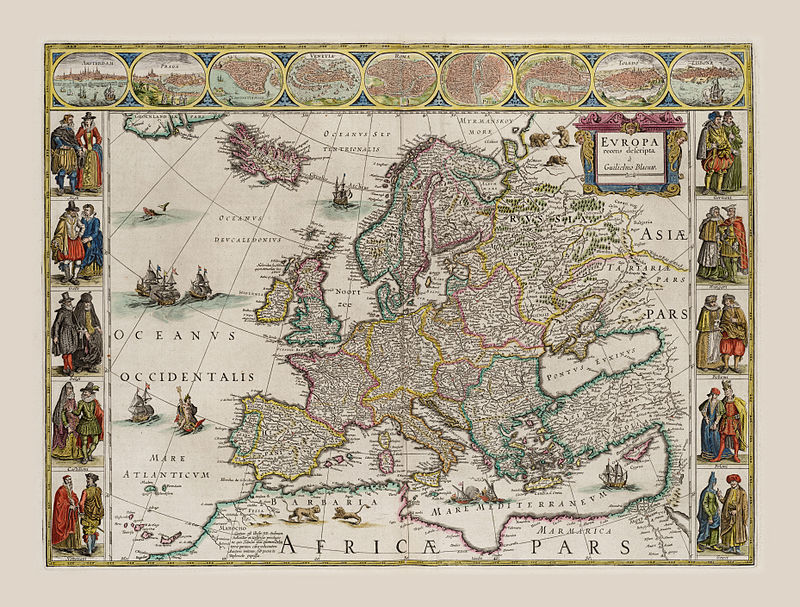
\includegraphics[width=1\textwidth]{figures/petadinding.jpg}	
\caption{Peta Dinding}	
\label{petadinding}
\end{figure}

gambar ini \ref{petadinding.jpg} merupakan peta yang dibuat oleh Willem Blaeu pada tahun 1640
 
Wieder Menjual Petanya dan Berhasil ditemukanya peta dinding oleh WillemJansz Bleau .Namun, artikel tersebut tidak menyebutkan lokasi peta dinding berada. 
Selama perang dunia kedua wieder menjual koleksi peta itu sendiri di berlin dimana ia hilang di dalam kekacauan. 
Sehingga sangat mungkin koleksi ini termasuk peta dinding dunia. tentang proyeksi mercator 1606 - 1607, 
karena dalam salinan pribadi kartografi monumenla ini (sekarang di pelihara di perpustakaan negara bagian barat berlin) 
dr. wieder di tandai dalam manuskrip - dengan catatan : 'sekarang peta ini selesai'. 


Di dalam biografi nya tentang willem jansz Blaeu 1932 , tapi tidak mungkin F. C. Wieder sudah merujuk pada adanya lembaran tangan dari 
peta ini di Museum Nasional Germanisches di Nurnberg. Sampai saat ini, investigasi di dasarkan pada lembar satu yang ini di Nurnberg dan deskripsi singkat dari Wieder yang menyebut peta ini sebagai monumen ukiran 
dan karya seni Belanda yang di ciptakan oleh seorang pria hebat dan berbudaya, sebuah monumen ilmiah yang luar biasa dari awal masa ‘colonial'. 
Sementara penulis saat ini sedang belajar di Rijksmuseum Nederlands Scheepvaart-Museum di Amsterdam, 
dia membolak-balik dua kotak foto peta yang di peroleh dalam sebuah lelang yang di adakan pada tahun 1958. 
'Betapa terkejut nya dia menemukan di antara foto-foto ini yang terpaku pada kardus gambar kecil ( 9 x 13 cm ) 
peta dinding dunia pada proyeksi Mercator oleh Willem Jansz Bleau dari tahun 1606 - 1607. 
Ini memberi kesan visual tentang keindahan asli bintang yang hilang ini. 
Gambar 1) dan memungkinkan deskripsi detail dari peta itu sendiri dan pengaruh nya terhadap peta dunia lain nya. 
Penulis buku ini mencoba membuat foto-foto kecil yang di perbesar oleh Layanan Topografi di Delft sampai ukuran seperti itu 
sehingga garis pantai bisa menjadi lebih jelas dan huruf iegen terbaca. 
Pembesaran ini membuat kontur pantai lebih jernih namun teks tetap tidak jelas. 
Untung nya, dengan mencari jalan ke berbagai peta dunia yang berasal dari Willem Jansz Bleau. 'peta dinding dia berhasil di patenkan. 

\cite{campbell1976descriptive}

\subsection{Karya Willem Blaeu}
Selama hampir 70 tahun, biografi Baudet Willem Jansz Bleau Maior sudah menjadi sumber utama untuk pengetahuan kita 
tentang kehidupan dalam karya willem jansz Blaeu's. Karena, bagaimana pun kurang nya sumber–sumber yang tersedia di tahun-tahun 
sebelum nya sudah di tangani sangat ringkas dalam karya tersebut. 
Ini khusus nya adalah kebenaran hubungan Brahe's dengan Tycho Brahe dan pelatihan yang diterima oleh Joll Ander muda dibawah bimbingan Brahe's pafa Hven. 
Pelatihan ini diketahui, dalam banyak cara untuk menentukan penting nya pekerjaan nanti nya dia di tanah sendiri. 
Pada tahun 1914 kehidupan dan pekerjaan willem jansz Baleu's akan diteliti dari awal oleh Stevenson, 
kalian ini dengan referensi khusus untuk karya nya, peta penting dunia 1605. Pekerjaan tidak berisi informasi lain yang bener-bener 
baru tentang hubungan willwm jansz Blaeu's dengan Brabe. Sejak hari Baudet's bagaimanapun, 
pengetahuan kita tentang kehidupan dan penelitian Brahe's sudah sangat meningkat. 
Dan telah memiliki sedikit bagian dalam hal ini. Pada tahun 1980 dreyer di terbitkan sejauh biografi paling rinci dan terbaik dari Brabe.  
Dreyer, salah satu sejarawan pembimbing astronomi di waktu kita dan dane, 
pada khusus nya di lengkapi untuk kumpulan karya Brahe's dan pada 1913 ia terbit di edisi jilis pertama dari Opera Omnia. 
Dua tahun setelah kematian nya, pada tahun 1928 pekerjaan selesai. 
Artinya dari koleksi surat ini dapat di tetapkan beberapa fakta lebih lanjut untuk tetap di Blaeu Hven dan pandangan sebelum nya di koreksi. 
Untuk jenis pengetahuan pelatihan dari Blaeu  di berikan pada Hven,
bagaimanapun penelitian masih harus mencari sumber utama dalam karya ilmiah umum dan praktis yang di lakukan disana. 

\cite{Richter1939Willem}


Hampir tidak memiliki brahe menetap dirinya di pulau kecil hven (kemudian yang dimiliki Denmark) Suara, 
yang ia telah diberikan pada 1576 oleh Fredrik II, raja Denmark dari laporan View baru astronom telah di rayakan dua ini telah menyebar ke luar negeri. 
Atau apakah itu lama sebelum orang - orang muda yang tertarik dari dekat dan jauh membuat mereka berada di sana sebagai murid-muridnya. 
Beberapa menjadi para pembantu nya. Dalam dua puluh tahun brahe tinggal di hven ada sebagai aturan enam sampai delapan. 
Kadang-kadang bahkan sebanyak sepuluh sampai dengan dua puluh, pria muda yang bekerja terus . 
Brahe membuat permintaan besar pada murid–murid nya. Beberapa yang ia di undang untuk datang; server lain ia pasti hanya mengambil rekomendasi khusus. 
Semua dianggap sebagai sebuah kehormatan yang besar untuk di izinkan untuk datang ke hven. 
Untuk pertanyaan apakah brahe dan Maior, mengingat pembentuk kematian awal sebagai 1601, 
bisa membentuk setiap persahabatan bertahun-tahun berdiri seperti yang sering di katakan di biografi data mengenai willwm jansz bleu. 
dan itu ada, tidak di ragukan lagi bahwa blaen, karena kemampuan ini, sekaligus memenangkan brahe's hal khusus. 
Ini mau menjadi bahwa brahe punya pengalaman baik orang Belanda muda dengan siapa ia datang ke dalam kontak pada hven, 
karena Maior tidak satu - satunya. Groningensis rudolphus tertentu ia di sebutkan dalam ini 1586 dan 1588 Meteorologi 
hari buku yang telah di pelihara dari tahun 1582 untuk 1597 pada hven. 
Pada 1590 tinggal pendek di buat tidak oleh Arnold Van langren, 
putra terkenal dunia penanda florentius Jacobus Van langren. 
Jacobus buruk mengirimnya ke brahe untuk meminta untuk akan di izinkan supaya bisa menyalin Katalog bintang brahe's, 
yang Jacobus berkeinginan untuk membuat penggunaan untuk bola langit. 

Ini mau menjadi bahwa brahe punya pengalaman baik orang Belanda muda dengan siapa ia datang ke dalam kontak pada hven, 
karena Maior tidak satu - satunya. Groningensis rudolphus tertentu ia di sebutkan dalam ini 1586 dan 1588 Meteorologi 
hari buku yang telah di pelihara dari tahun 1582 untuk 1597 pada hven. 
Pada 1590 tinggal pendek di buat tidak oleh Arnold Van langren, 
putra terkenal dunia penanda florentius Jacobus Van langren. 
Jacobus buruk mengirimnya ke brahe untuk meminta untuk akan di izinkan supaya bisa menyalin Katalog bintang brahe's, 
yang Jacobus berkeinginan untuk membuat penggunaan untuk bola langit. 
\cite{Richter1939Willem}





\chapter[Pendahuluan]
{Pendahuluan\\ definisi}
% kelompok definisi
% ariana setiawan (1154042)
% idang mawardi (1154084)
% arya niken manalu (1154080)
% M. Arya Sikumbang (1154075)
% r rifa fauzi komara (1154089)
% Andi Tenri Wali (1154013)

\section{Definisi GIS (GEOGRAPHICS INFORMATION SYSTEM)}
Geographical information system (GIS) adalah sebuah komputer yang berbasis sistem
informasi digunakan untuk memberikan informasi bentuk digital dan analisa terhadap 
permukaan geografi bumi.

\subsection{Pemahaman pada Geographics Information System GIS}
Dimana GIS merupakan pemahaman dari, sebagai berikut:
\begin{enumerate}
\item Geography

Dimana GIS dibangun berdasarkan pada istilah‘geografi’ atau ‘spasial’.
Object mengacu pada spesifikasi lokasi dalam suatu tempat/ruang. Objek dapat berupa fisik,
budaya ataupun ekonomi alamiah. Penampakan yang seperti ini ditampilkan pada suatu peta yang 
digunakan untuk memberikan gambaran yang lebih representatif dari spasial dari suatu objek.
sesuai dengan kenyataannya yang di bumi. Dimana simbol, warna dan gaya garis digunakan sebagai
perwakilan dari setiap spasial yang berbeda pada peta dua dimensi.
Pada gambar \ref{dataspasial} dijelaskan bahwa data spasial berikut berupa 
titik, garis, poligon (2-D) dan permukaan (3-D).

\begin{figure}[ht]
	\centerline{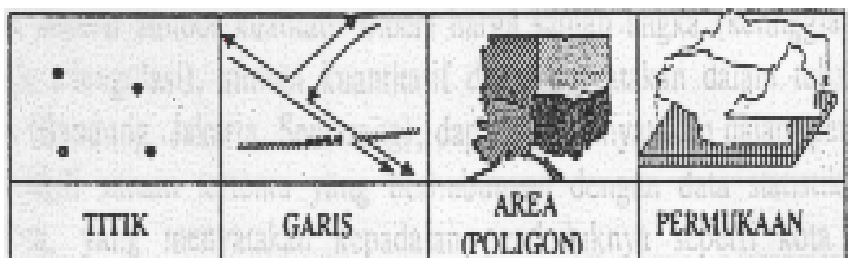
\includegraphics[width=1\textwidth]{figures/dataspasial.JPEG}}
	\caption{data spasial berikut berupa titik, garis, poligon (2-D), permukaan (3-D).}
	\label{dataspasial}
	\end{figure}

Dan arti dari gambar diatas adalah :
Format Titik 						
- Memiliki koordinat tunggal 		
- Tanpa memiliki panjang 			
- Tanpa memiliki luasan

Format Garis
- memiliki koordinat titik awal dan akhir		
- memiliki panjang tanpa luasan

Format Poligon 					
- memiliki koordinat titik awal dan akhir
-memiliki panjang dan luasan 		

Format Permukaan
- memiliki area koordinat vertikal
- memiliki area dengan ketinggian

\item Information
Informasi berasal dari kata pengolahan sejumlah data. Di dalam GIS informasi mempunyai
volume terbesar. Dan setiap object geografi memiliki setting datanya tersendiri karena 
tidak sepenuhnya data yang ada dapat terwakili didalam peta. Maka, semua data harus
diasosiasikan pada objek spasial yang mampu membuat peta menjadi intelligent.

\item System
Pengertian dari suatu sistem merupakan kumpulan elemen-elemen yang saling berintegrasi 
dan berinterdependensi dalam sebuah lingkungan yang dinamis untuk mencapai tujuan tertentu.
\end{enumerate}

\subsection{Definisi GIS (Geography Information and System)}
Dan defenisi dari GIS dapat selalu berubah karena GIS adalah bidang kajian ilmu 
dan teknologi yang masih baru. Beberapa defenisi dari Geographical Information System yaitu:
\begin{enumerate}
\item Definisi GIS menurut(Rhind, 1988):
yaitu : GIS is a computer system for collecting, checking, integrating and analyzing
information related to the surface of the earth.

\item Definisi GIS menurut(Marble \& Peuquet, 1983) and (Parker,
1988; Ozemoy et al., 1981; Burrough, 1986):
yaitu : GIS deals with space-time data and often but not necessarily, employs computer
hardware and software.

\item Difinisi GIS menurut (Purwadhi, 1994):
- SIG adalah suatu sistem yang mampu mengorganisir perangkat keras (hardware),
perangkat lunak (software), dan data, serta dapat mendaya dan digunakan sistem
penyimpanan, pengolahan, maupun analisis data yang dilakukan secara simultan, sehingga dapat
diperoleh seluruh informasi yang berkaitan secara langsung dengan aspek keruangan.
- SIG adalah manajemen data spasial dan data non-spasial yang berbasis komputer
dengan menggunakan tiga karakteristik dasar, yaitu: 
(i) memiliki fenomena yang aktual (variabel data non-lokasi) dan berhubungan 
dengan topik permasalahan di lokasi bersangkutan; 
(ii) merupakan suatu kejadian di suatu lokasi tertentu; 
(iii) memiliki dimensi waktu. Alasan GIS dibutuhkan adalah karena untuk data spasial 
penanganannya sangat sulit karena peta dan data statistik cepat mengalami kadaluarsa 
sehingga tidak ada pelayanan penyediaan data dan informasi yang diberikan menjadi tidak akurat.
\end{enumerate} 

Berikut merupakan keistimewaan analisa dengan Geographical Information System (GIS) yaitu:
\begin{enumerate}
\item Analisa Proximity
Analisa Proximity adalah geografi yang berbasis pada jarak antar layer.
Didalam analisis proximity GIS menggunakan proses yang disebut dengan buffering
yaitu membangun lapisan pendukung sekitar layer dalam jarak tertentu agar dapat menentukan
dekatnya hugungan antara sifat bagian yang ada.
\item Analisa Overlay
Analisa Overlay adalah proses integrasi data dari lapisan-lapisan layer yang berbeda (overlay).
Yang secara analisa membutuhkan lebih dari satu layer yang akan ditumpang susun secara
fisik agar dapat dianalisa secara visual.
\end{enumerate}

Maka artikel :
	Dalam sebuah artikel dari husein yang menyebutkan bahwa  GIS merupakan pemahaman dari
	Geography, Information dan System \cite{husein2006konsep}.

\section{Geographic Information System (GIS): Introduction to the computer perspective}
Sistem Informasi Geografi (GIS) diartikan sebagai sistem untuk menyimpan, memeriksa, 
mengintegrasi, memanipulasi, menganalisis dan memaparkan data yang berkaitan dengan semua 
ruang yang berhubungan dengan keadaan bumi.
Maka artikel :
	Dalam sebuah artikel dari prahasta yang menyebutkan bahwa  GIS merupakan menyimpan, memeriksa, mengintegrasi, memanipulasi, menganalisis dan memaparkan data yang berkaitan dengan semua ruang yang berhubungan dengan keadaan bumi., Information dan System \cite{prahasta2009sistem}.

\subsection{Pengenalan GIS atau Geography Information System}
1. GIS atau dikenal dengan Sistem Informasi Geografi ditunjukan sebagai sistem yang mampu menyimpan, memeriksa, mengintegrasikan, memanipulasi, menganalisis dan memaparkan data-data yang terkait dengan spasial yang merunjuk terhadap bagian bumi. (Jabatan Alam Sekitar, 1987).

2. GIS merupakan satu set lat untuk mengumpulkan, menyimpan, mendapatkan, mengubah dan memaparkan data ruang dari keadaan  bumi yang sebenarnya untuk keperluan tertentu (Burrough, 1986).

3. GIS adalah setiap set manual atau prosedur komputer yang digunakan untuk menyimpan dan memanipulasi data geografis yang tersedia (Arronoff, 1989).

4. GIS merangkum keadaan bumi dengan peranti atau perangkat tertentu yang digunakan untuk peta input atau peta produk, bersama-sama dengan dengan sistem komunikasi yang diperlukan untuk dijadikan sebagai penghubung berbagai unsur. (Star \& Ester, 1990).

5. GIS adalah suatu sistem untuk membantu dalam membangunkan model tertentu yang mustahil untuk dijadikan sintesi data yang banyak. (Martin, 1996).

\subsection{Komponen GIS atau Geography Information System}
Komponen GIS sendiri dibagikan menjadi 3 komponen, yaitu :
Sistem Komputer (perkakas dan sistem operasi), Software GIS
(ArcGIS), database GIS, methode GIS (Prosedur analisis), People (Orang-orang yang menggunakan GIS/User).
Pada gambar \ref{komponenGIS} dijelaskan bahwa kompnen GIS sebagai berikut.

\begin{figure}[ht]
	\centerline{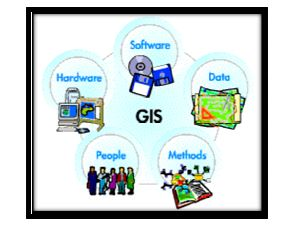
\includegraphics[width=1\textwidth]{figures/komponenGIS.JPG}}
	\caption{komponen GIS.}
	\label{komponenGIS}
	\end{figure}

\subsubsection{Komponen GIS atau Geography Information System}
sesuai dengan gambar diatas komponen GIS dibagi menjadi 3 bagian, yaitu :
1. Sistem Komputer (perkakas dan sistem operasi), merupakan hardware dari sebuah sistem GIS. Perkakas terdiri dari monitor, unit sistem atau CPU, keyboard dan mouse (Heywood et al., 2002). Teknologi komputer harus memiliki kemampuan kuasa
yang tinggi untuk menjalankan perisian GIS.

2. Software GIS , merupakan ArcGIS untuk tujuan perancangan, pengurusan ataupun pemodelan pada kebutuhan tertentu.

3. Database GIS , merupakan tempat yang melibatkan data GIS baik data spatial dan pengurusan datanya. memori untuk menyimpan jumlah data yang besar dan mempunyai kualitas yang baik dengan resolusi tinggi pada skrin grafik warna (untuk membantu dalam menentukan maklumat yang dihasilkan atau diberikan melalui penggunaan warna yang berbeda).

4. Methode GIS , merupakan prosedur dari analisis sistem GIS. yang melibatkan proses input, proses menyimpan, proses mengurus, proses menukar, proses menganalisis, dan proses output yang hanya melibatkan perisian GIS untuk mengatur sistem dan data-data tersebut (Heywood et al., 2002 )

5. People , merupakan orang-orang yang menggunakan sistem GIS. atau orang yang mengendaliakn proses input-output sistem GIS. 

\subsection{Kaedah GIS atau Geography Information System}
Berdasarkan pemahaman diatas, kaedah GIS juga merupakan salah satu komponen penting untuk mengatur sistem GIS sesuai dengan penjelasan sebelumnya. Kaedah-kaedah ini terdiri dari input
data spatial, pengurusan data atribut, paparan data, penerokaan data, analisis dan pemodelan data GIS;
yang dijelaskan oleh gambar sebagai berikut:
Pada gambar \ref{kaedahGIS} dijelaskan bahwa kaedah GIS sebagai berikut.
\begin{figure}[ht]
	\centerline{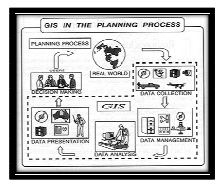
\includegraphics[width=1\textwidth]{figures/kaedahGIS.JPG}}
	\caption{kaedah GIS.}
	\label{kaedahGIS}
	\end{figure}

\subsubsection{Kaedah GIS atau Geography Information System}
1. Input data spatial
Merupakan langkah awal agar terciptanya data baru, dengan cara menginputkan data dan sistem GIS akan menyuntingnya dalam bentuk transformasi geometri yang nantinya akan menghasilkannya kedalam bentuk hard copy. (Chang, 2008) 
(Heywood et al., 2002).

2. Pengurusan data artibut
Merupakan langkah selanjutnya agar sumber peta dapat dipindahkan kepada peta digital yang dapat dibaca oleh GIS.
(Chang, 2008) (Worboy \& Duckham, 2003) (Heywood et al., 2002)

3. Pengumpulan data
Merupakan aktivitas untuk proses melakukan eksplorasi lebih jauh dalam meneliti ciri kesamaa dalam suatu graf peta yang berbeda. (Worboy \& Duckham, 2003).

4. Analisis data
Merupakan cara untuk memaparkan dan memanipulasi data yang didapat. Dengan menggunakan 2 jenis format, yaitu :
- data vektor : melibatkan beberapa kaedah seperti penimbalan / buffering, penindihan/overlay, pengukuran jarak, statik ruang, dan manipulasi peta.
- data raster : menaganalisis pengumpulan data tempatan, kaedah kejiranan, kaedah berzon, dan kaedah operasi global.
(Chang, 2008) (Worboy \& Duckham, 2003) (Heywood et al., 2002)

5. Paparan data dan output data
Dasarnya disediakan untuk tujuan pemaparan hasil dari analisis data yang fungsinya ditujukan untuk pengguna.

6. Aplikasi GIS
Digunakan untuk keperluan tertentu dan bersifat umum bagi masyarakat tergantung keperluan penggunanya. 
(Heywood et al., 2002).

Pada gambar \ref{aplikasiGIS} dijelaskan bahwa aplikasi GIS sesuai keperluan penggunan sebagai berikut.
\begin{figure}[ht]
	\centerline{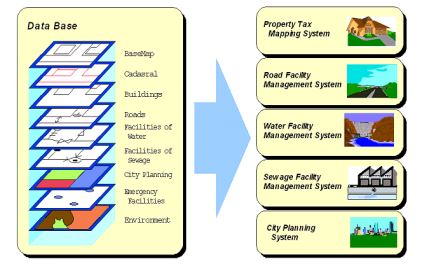
\includegraphics[width=1\textwidth]{figures/aplikasiGIS.JPG}}
	\caption{aplikasi GIS.}
	\label{aplikasiGIS}
	\end{figure}
Maka artikel :
	Dalam sebuah artikel dari hua yang menyebutkan bahwa  GIS memiliki kaedah dan komponen, Information dan System \cite{hua2017sistem}.

\subsection{Kesimpulan GIS atau Geography Information System}
Kesimpulannya, GIS merupakan alat yang penting dalam perspektif komputer pada masa kini dikarenakan GIS
mempunyai kemampuan aplikasi dalam berbagai bidang, misalnya dalam proses perancangan bandar dan kartografi,
penilaian kesan alam sekitar dan pengurusan sumber asli. GIS juga memainkan peranan dalam perspektif perniagaan,
dimana alat ini sangat bermanfaat dalam pengiklanan dan pemasaran, jualan, dan logistik 
mampu digunakan untuk mencari dan meningkatkan perniagaan seperti tapak perniagaan yang strategik. Sebagai umum, pengguna GIS dapat dilibatkan dengan agensi-agensi penguatkuasaan undang-undang, strategi
perancangan, perhutanan, industri, pemberdayaan alam, perencanaan kota, profesional
telekomunikasi, kesehatan, pengangkutan, geografi, dan pembangunan pemasaran. 
Penjelasan ini menyediakan platform untuk memahami lebih lanjut tentang komponen, kaedah, dan aplikasi GIS, 
untuk mempelajari tentang alat GIS.
\subsection{Saran GIS atau Geography Information System}
GIS dapat diaplikasikan di dalam kehidupan sehari-hari untuk memenuhi kebutuhan dan dapat membantu kebutuhan setiap masyarakat menjadi lebih baik dan lebih bermanfaat. Karena dengan memanfaatkan kemajuan teknologi maka teknologi yang digunakan akan ikut turut serta terus perkembang untuk menyesuaikan pemenuhan kebutuhan setiap pengguna yaitu masyarakat. Demikian kesimpulan dan saran yang dapat disampaikan kurang lebihnya mohon maaf dan terimakasih.

\subsection{SIG mempresentasikan real world dengan data spasial yang terbagi atas 2 model data, yaitu:}
1. Vektor, Bumi dalam data vector direpresentasikan sebagai mozaik yang terdiri atas garis, polygon, titik,
dan noders.
Model data vector merupakan model data yang paling banyak digunakan, model ini berbasiskan
pada titik dengan koordinat (x,y) untuk membangun objek spasialnya. Objek yang dibangun
dibagi menjadi tiga bagian, yaitu: titik, garis, dan area (polygon).
Keuntungan dari data vector, yaitu: ketepatan dalam merepresentasikan fitur titik, batasan dan
garis lurus.
2. Raster, Data raster adalah data yang dihasilkan dari sistem pengindraan yang jauh. Pada data raster,
objek geografis direpresentasikan sebagai struktur sel grid yang disebut pixel. Resolusi pada data
raster tergantung pada ukuran pixel-nya.
Maka, resolusi pixel menggambarkan ukuran sebenarnya dari permukaan bumi yang diwakili
oleh setiap pixel pada citra. Semakin tinggi resolusinya, semakin kecil permukaan bumi yang
direpresentasikan oleh suatu sel. Data raster cocok untuk merepresentasikan batas-batas yang
berubah secara gradual, seperti jenis tanah, vegetasi, suhu tanah, dan kelembaban tanah.


\chapter[Sejarah Kutub Utara]
{Pengantar\\ Kutub Utara}
%Kelompok 3
%Kutub Utara
%
%Andi Syahjaratu Daur - 1154092
%Aditya Pratama Dharma - 1154043
%Bendra Wardhana - 1154015
%Dini Islamiani - 1154039
%Nur Rahmawati - 1154124	
%Pembahasan Dan Isi 

\section{Deskripsi Kutub Utara}	

		Dalam artikel Arctic Monitoring and Assessment Programme {AMAP}  ada beberapa masalah yang ada didalam 
	kutub utara, yang paling menonjol adalah masalah polusi dan lingkungan.
		
		Kutub Utara sedang mengalami beberapa hal yang paling cepat dan perubahan iklim berat di bumi. Selama 100 tahun,perubahan
	iklim diharapkan untuk mempercepat, memberikan kontribusi untuk fisik utama, ekologi, sosial, dan perubahan ekonomi, banyak yang 
	telah dimulai. Perubahan iklim kutub utara juga akan mempengaruhi seluruh dunia melalui peningkatan pemanasan global dan meningkatnya permukaan laut. 
	Dampak dari Kutub Utara merupakan dataran tinggi penghangat sintesis bahasa dari temuan-temuan kunci Kutub Utara Dampak Perubahan Iklim {ACIA}, dirancang 
	untuk dapat diakses untuk para pembuat kebijakan dan publik yang lebih luas. Dalam ACIA adalah secara komprehensif diteliti, benar-benar direferensikan,
	dan evaluasi secara independen dari perubahan iklim kutub utara. Ia telah terlibat sebuah upaya internasional oleh ratusan ilmuwan.
	Dalam artikel Impacts of a Warming Arctic - Arctic Climate Impact Assessment ini menyediakan informasi penting kepada masyarakat dan contemplates-respons 
	untuk salah satu tantangan terbesar pada zaman kita.
	
		Northeast Rusia, dan sungai Mackenzie {130 W. panjang.}, Amerika Barat Laut, dan antara Laut Arctic di utara dan selatan Alaska dan
	Kuriles tengah di selatan. Wilayah ini disajikan sebagai suatu negeri-jembatan antara Eurasia dan Amerika Utara di seluruh Tertiary sehingga kira-kira 5 Ma
	ketika ia diputuskan oleh pembentukan Bering Strait {Marincovich \& Gladenkov 1999, 2001}. Selama Kuartenari, tanah-pembaharuan bridge selama glaciations 
	utama bila tingkat laut jatuh oleh 100-135 m {Hopkins 1973; Clark \& Mencampur 2002}.Northeast Rusia dan Amerika Barat Laut {Alaska dan Yukon} tetap bebas es 
	selama Kuartenari glaciations dan melayani sebagai refugium utara besar-besaran untuk kutub utara dan boreal biota.Wilayah ini Beringia Hultén dipanggil dan
	didefinisikan sebagai kawasan antara Sungai Lena {125 E. panjang.}, Northeast Rusia, dan sungai Mackenzie{130 W. panjang.}, 
	Amerika Barat Laut, dan antara Laut Arctic di utara dan selatan Alaska dan Kuriles tengah di selatan.Wilayah ini disajikan sebagai suatu negeri-jembatan antara 
	Eurasia dan Amerika Utara di seluruh Tertiary sehingga kira-kira 5 Ma ketika ia diputuskan oleh pembentukan Bering Strait {Marincovich \& Gladenkov 1999, 2001}. 
	Selama Kuartenari, tanah-pembaharuan bridge selama glaciations utama bila tingkat laut jatuh oleh 100-135 m {Hopkins 1973; Clark \& Mencampur 2002}.
	
\subsection{Kutub Utara Tahun ini}

		Dalam Kuartenari {kira-kira 2 Ma hingga sekarang} distribusi dan komposisi kutub utara flora ini sangat dipengaruhi oleh terlebih dahulu dan mundur dari 
	lapisan-lapisan ais. Secara tradisional, ia berpikir bahwa selama periode seretnya proses semua wilayah utara tertutup oleh es ke sejauh serupa dan bahwa
	binatang dan tumbuhan kutub utara bermigrasi ke selatan memajukan lembaran-es untuk bertahan hidup di selatan refugia {Darwin tahun 1859; Hooker tahun 1862}.
	Namun, keyakinan ini menghadapi tantangan dalam 1937 oleh bahasa Swedia botanis, Eric Hultén, dalam bukunya garis besar tentang sejarah Kutub Utara dan 
	Boreal Biota selama periode divisi kuartenari. Hultén menarik pada bukti geologi dan tubuh yang luas dari bukti phytogeographical sendiri, untuk mengusulkan
	bahwa kebanyakan dari Northeast Rusia dan Amerika Barat Laut {Alaska dan Yukon} tetap bebas es selama Kuartenari glaciations dan melayani sebagai refugium 
	utara besar-besaran untuk kutub utara dan boreal biota {Gbr. 1}. Wilayah ini Beringia Hultén dipanggil dan didefinisikan sebagai kawasan antara Sungai Lena 
	{125 E. panjang.}
		Kutub Utara tahun ini terdiri dari kira-kira 1.500 spesies flora dan yang relatif baru asal usul {Murray 1995}. Perguruan Tinggi di sebagian besar {65-2 Ma}, 
	hutan tumbuh di ketika latitud tinggi di Kutub Utara {Murray 1995; McIver \& Basinger 1999} dan tundra tidak muncul hingga akhir Pliocene {Salasila Matius \& Ovenden 1990}.
	Pada awalnya tundra ini disebarluaskan discontinuously, tetapi sebuah sabuk circumarctic hadir dengan 3 Ma {Salasila Matius 1979}. 
	Sedikit yang diketahui tentang asal usul tumbuhan kutub utara, walaupun ianya diandaikan bahawa banyak tanaman tersebut berasal dari saham nenek moyang yang terjadi 
	di gunung-gunung yang tinggi, di sebelah selatan di Asia dan Amerika Utara {Hultén 1937; Tolmachev 1960; Weber 1965; Hedberg 1992; Murray 1995}. Gunung ini membentuk 
	bagian dari berkisar antara terhubung ke Kutub Utara, di sepanjang tanaman yang dapat bermigrasi ke arah utara, seperti suhu global turun secara signifikan dari 
	pertengahan Miocene dan seterusnya {Lear et al. 2000; Zachos et al. 2001}. Selain itu, beberapa tanaman kutub utara mungkin berasal dari shrubby dan elemen-elemen 
	herbaceous hutan kutub utara yang menduduki Tersier membuka, dan riparian {40-2}-habis sama sekali habitat dataran tinggi di Kutub Utara selama akhir 
	Tertiary {Murray 1995}.
	
\begin{figure}[ht]
\centerline{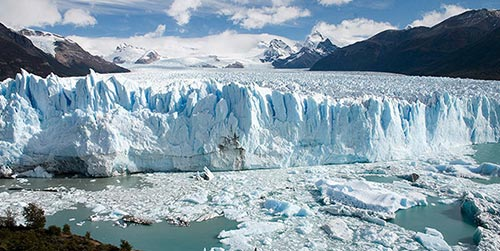
\includegraphics[width=1\textwidth]{figures/arctic.jpg}}
\caption{Menjeleskan tentang kutub utara.}	
\label{Kutub_Utara}
\end{figure}
	
\subsection{Pemanasan di kutub utara}
		Metana di dalam atmosfir kutub utara telah meningkat dengan tajam sebanyak 33% dalam kurun 5 tahun tanah es yang mencair di siberia telah melepaskan 5x 
	jumlah metana dari yang sebelum nya di prediksi permafrost dangkal bawah laut pada kutub utara juga menunjukan ketidak stabilan dan melepaskan jumlah metana
	yang banyak padang rumput pada kutub utara pada saat ini sudah mengeluarkan lebih banyak metana dan nitrogen oksida dari perkiraan yang sebelumnya ilmuan 
	telah memberi nama pencairan kutub utara dengan nama bom waktu yang berdetak, Kutub utara memanas dua kali lebih cepat di bandingkan tempat lain yang berada
	di bumi tanpa es yang melindungi untuk memantulkan sinar matahari , di dunia terdapat dua lapisan es besar yaitu greenland dan kutub selatan Kutub utara merupakan
	negara yang mustahil untuk di tempati makhluk hidup namun juga terdapat beberapa spesies fauna yang dapat hidup disana salah satu nya adalah beruang kutub
	meski memiliki tubuh yang besar beruang kutub mampu berenang selama berhari-hari di perairan terbuka dan sanggup menjangkau jarak ratusan kilometer .

\begin{figure}[ht]
\centerline{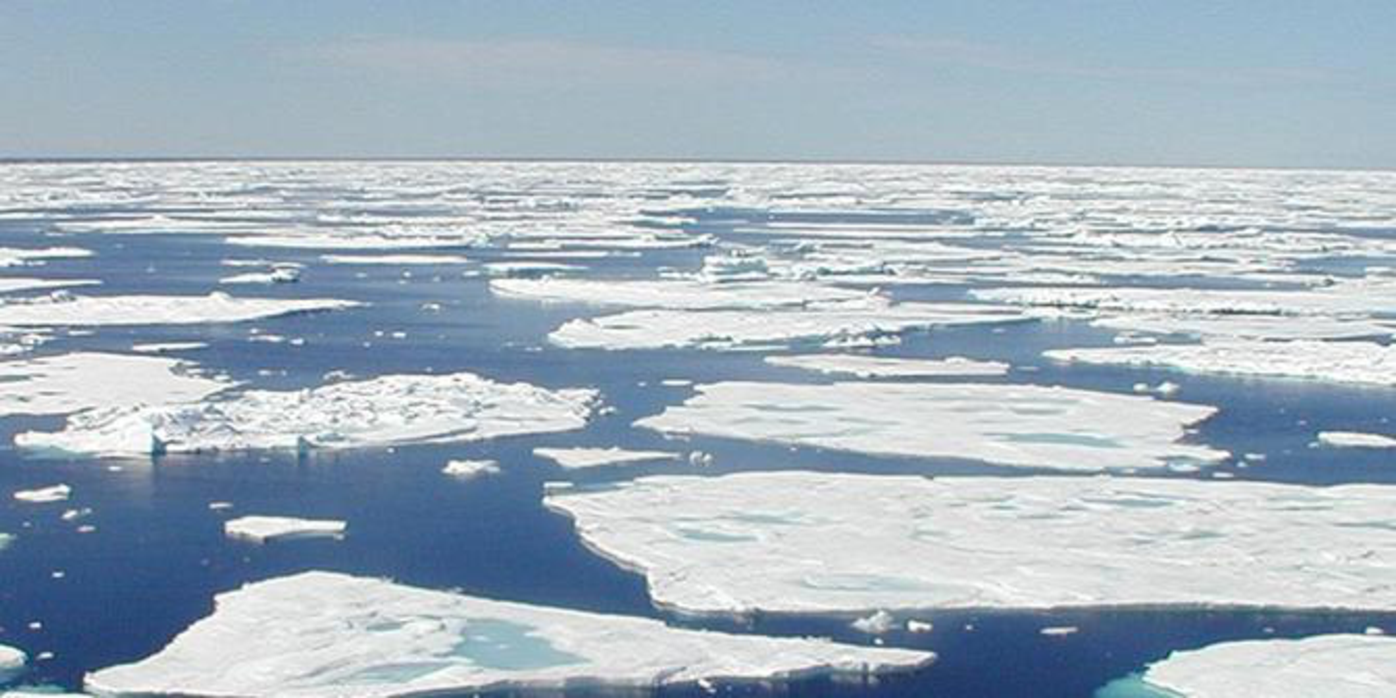
\includegraphics[width=0.5\textwidth]{figures/arctic1.pdf}}
\caption{Menjeleskan tentang pemanasan kutub utara.}	
\label{Pemanasan_Kutub_Utara}
\end{figure}

Pada gambar \ref{Pemanasan_Kutub_Utara} menjelaskan tentang pemanasan di kutub utara.

\subsection	{Kutub Utara}	ari 2 meter lebih pada 50 tahun 
	mendatang. Upaya untuk mengatasi tantangan perubahan iklimdan kenaikan permukaan laut tersebut, kota Rotterdam telah membangun beberapa struktur terapung 
	berdesain unik dan menarik, Dan Menurut nanang rianto dampak pencairan es di Kutub Utara dan Selatan akibat pemanasan global,dan gejala penurunan elevasi
	tanah (land subsidence).
	
		Kutub utara diramalkan akan punah karena habitatnya yang mengecil.bobot hewan itu mengalami penyusutan signifikan dalam dekade
	akhir ini.Makanan beruang adalah ikan,Mereka mencarinya dengan membuat lubang di lapisan es sehingga ketika ada ikan lewat langsung disambarnya.sekarang 
	jangankan membuat lubang mencari tempat berpijak saja susah karena banyaknya es yang mencair sehingga beruang harus sering melompat berpindah balok es.
	Tak jarang pun ikan susah ditangkap.beruang kutub harus berenang bermil-mil demi mendapatkan tempat baru, dan ini berisiko besar karena domain beruang
	kutub bukanlah dilaut.
	
	
\subsubsection {Kutub Utara}
		Kutub utara magnet bumi untuk diinterpretasi. Hasil interpretasi kualitatif menunjukkan bahwa pada peta anomali regional terdapat anomali dipole magnetik
	yang membentang dari arah barat daya ke timur laut Semenanjung Muria, Peta anomali lokal menunjukkan dua buah anomali dipole magnetik yang membentang dari 
	arah barat laut ke tenggara di sebelah utara dan barat kompleks Gunungapi Muria, dan satu pasang dipole magnetik di tenggara Gunungapi Muria Hasil 
	interpretasi kuantitatif yang dilakukan dengan menggunakan software Mag2DC for Windows. Pada anomali regional dan anomali lokal yang direduksi ke kutub 
	terdapat sebuah sesar di sebelah tenggara gunungapi Muria, tepatnya pada daerah Maar Gunung Rowo. Struktur geologi bawah permukaan daerah Gunungapi Muria 
	dan Maar Gunung Rowo berdasarkan harga suseptibilitas batuan dikontrol oleh batuan vulkanik yang terdiri dari andesit dari satuan batuan Lava Muria, tufa 
	dari satuan batuan Tuf Muria, batupasir tufaan dari formasi Patiayam, batugamping dari formasi Bulu, dan batulempung dari formasi Ngrayong. Pada kedalaman
	7-15 km di bawah permukaan terdapat batuan vulkanik dan vulkanik klastik yang merupakan batuan dasar penyusun Semenanjung Muria.
	
\subsubsection{kutub utara magnet diinterpretasi}
		Kutub utara magnet bumi untuk diinterpretasi. Hasil interpretasi kualitatif menunjukkan bahwa pada peta anomali regional terdapat anomali dipole 
	magnetik yang membentang dari arah barat daya ke timur laut Semenanjung Muria, Peta anomali lokal menunjukkan dua buah anomali dipole magnetik yang 
	membentang dari arah barat laut ke tenggara di sebelah utara dan barat kompleks Gunungapi Muria, dan satu pasang dipole magnetik di tenggara Gunungapi
	Muria Hasil interpretasi kuantitatif yang dilakukan dengan menggunakan software Mag2DC for Windows. Pada anomali regional dan anomali lokal yang direduksi
	ke kutub terdapat sebuah sesar di sebelah tenggara gunungapi Muria, tepatnya pada daerah Maar Gunung Rowo. Struktur geologi bawah permukaan daerah 
	Gunungapi Muria dan Maar Gunung Rowo berdasarkan harga suseptibilitas batuan dikontrol oleh batuan vulkanik yang terdiri dari andesit dari 
	satuan batuan Lava Muria, tufa dari satuan batuan Tuf Muria, batupasir tufaan dari formasi Patiayam, batugamping dari formasi Bulu, dan 
	batulempung dari formasi Ngrayong. Pada kedalaman 7-15 km di bawah permukaan terdapat batuan vulkanik dan vulkanik klastik yang merupakan 
	batuan dasar penyusun Semenanjung Muria.
	
\subsubsection {kutub utara terendam}
		Menurut artikel Fatmasari Savitri, Eddy Prianto, Erni Setyowati i kutub utara dan selatan bumi akan terendam lebih dari 2 meter lebih pada 50 
	tahun mendatang. Upaya untuk mengatasi tantangan perubahan iklim dan kenaikan permukaan laut tersebut, kota Rotterdam telah membangun beberapa 
	struktur terapung berdesain unik dan menarik. 
	
\subsubsection {kepunahan habitat kutub utara}
		Kutub utara diramalkan akan punah karena habitatnya yang mengecil.bobot hewan itu mengalami penyusutan signifikan dalam dekade akhir ini.
	Makanan beruang adalah ikan,Mereka mencarinya dengan membuat lubang di lapisan es sehingga ketika ada ikan lewat langsung disambarnya.sekarang 
	jangankan membuat lubang mencari tempat berpijak saja susah karena banyaknya es yang mencair sehingga beruang harus sering melompat berpindah 
	balok es.Tak jarang pun ikan susah ditangkap.beruang kutub harus berenang bermil-mil demi mendapatkan tempat baru, dan ini berisiko besar karena 
	domain beruang kutub bukanlah dilaut.
	
		




\chapter[Tentang Kutub Selatan]
{Pengantar\\ Antartika}
%Kelompok 2
%DONI SAPUTRA(1154030)
%CAHYA KURNIAWAN(1154038)
%IKA SYAM SETIAWATI(1154054)
%SILVY DHARMA FEBRYANA(1154112)
%WIDI DAMAYANTI(1154062)
%ANTARTIKA


																		
Pembahasan Dan Isi 

\begin{figure}{ht}
\centerline{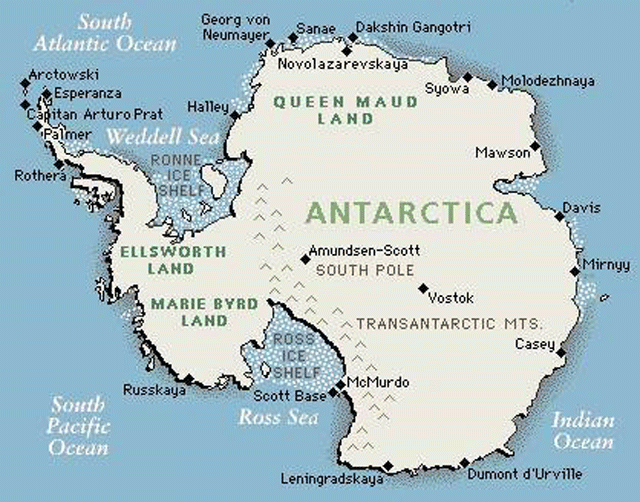
\includegraphics[width=1\textwidth]{figures/antartic.PNG}}
\caption{Menjelaskan tentang benua antartika.}
\label{Antartika}
\end{figure}

\section{Deskripsi Antartika}



		Benua antartika adalah suatu wilayah laut perifer yang merupakan sumber informasi utama pada cryosphere cenozoik dan peristiwa 
	kejadian yang mengarah pada perkembangan kurang lebih 36 juta tahun yang lalu. Dilihat dari berbagai data sekarang sudah terlihat bahwasanya 
	garis lintang selatan sudah mengalami perubahan dinamika ekspansi pada lapisan lapisan es nya dan pembusukan melewati akhir Palaeogene dan Neogene. 
	Pada ejarah perubahan iklim disertai dan sangat di pengaruhi oleh lithosphere vertical dan horizontal yang sangat signifikan. Peristiwa perubahan, 
	termasuk evolusi seaways internal utama dan pegunungan. \ref{Antartika}
		
		Meskipun penyidikan yang dilakukan di tahun pertama pada abad ini antartika kenozoikum penelitian ini adalah bagian dari beberapa kegiatan yang 
	relative memanjang di sedikit lebih dari 3 dekade di bagian lain dari bumi, kenozoikum rentan terhadap satu penyeledikan, dan dalam sejumlah perkara, 
	hampir 2 abad. Situasi ini sebagian besar dari bagian antartica. Yang sulit adalah penelitian lingkungan, keterbatasan peanfaatan teknologi canggih, 
	dan realisasi tertunda. Sebagai pentingnya selat lintang selatan yang tinggi untuk isu-isu global, tektonik evolusi seperti  palaeogeography, 
	palaeo-oceanography, biogeography, evolusi, dan palaeoclimate biotik. Meskipun komprehensif tinjauan kenozoikum sekarang sudah membuat penampilan yang baru 
	tetapi 25 tahun lalu konozoikum geologi dari antartika hanya mampu melayani beberapa saja.
	
		Terdapat perbedaan yang menarik dalam cara di mana dan kenozoikum pre-cenozoic studi yang telah dikembangkan di antartika.
	Penelitian dan pendalaman palaeozoic di mesozoikum dan gondwana  geologi yang berfungsi sebagai contoh yang baik .Pada akhir 1950s , 
	ahli geologi banyak dari negara negara berkumpul di antartika dengan cukup detail stratigraphic palaeontological dan informasi dan banyak pengalaman 
	dari banyak tahun penelitian di satu fragmen mantan supercontinent gondwana.Dalam hal kotor, para palaeozoic-mesozoic stratigraphy antartika 
	cermin melaporkan bahwa dari afrika selatan , india , australia , dan amerika selatan .Antartika palaeozoic-mesozoic disebut ilmu pengetahuan untuk 
	memberikan untuk mengukur daerah , stratigraphy , koleksi fosil , analisis dan batuan beku sedimen batu dan daerah analisis .Kebanyakan gondwanas  
	para ilmuwan itu , lalu , pengujian dan memperluas pengetahuan dasar yang itu , dalam banyak hal , dikembangkan di beberapa benua. 
	Fosil yang dikumpulkan di Antartika selama 30 tahun telah didokumentasikan dengan baik di wilayah-wilayah lain Gondwana dan penemuan mereka di Antartika 
	telah sering agak tepat memperkirakan. 
	
		Misalnya, dalam sebuah pra-Geofisik Internasional kaji ulang tahun, Fairbridge geologi Antartik (1952, mukasurat 88) dicatatkan, 
	"Maukah membingungkan dari semua adalah ketiadaan bukti seretnya proses di gunung batu zaman Permian, yang merupakan kali mengalami Glaciation 
	kuat dalam semua bagian lain di Selatan Hemi-; mengapa sphere Antartika, dari segala tempat akan dikecualikan.' Dalam satu dekade laporan-laporan 
	sebagai-ke-kemudian hilang tillites dibuat dari Rambu Supergroup dari Trans- Gunung dan lain-lain tempat Antartika. Elemen penting dalam kemajuan yang 
	dibuat oleh Palaeozoic cepat dan para peneliti Mesozoikum adalah mendukung pro- vided oleh IUGS Sub-Commission untuk Gondwana Stratigraphy serta 
	palaeontologi. Para peneliti Cenozoic Antartik tidak memiliki dukungan dari sebuah organisasi payung, walaupun IUGS Kuartenari Internasional Association 
	mungkin telah memainkan peran lebih aktif, terutama di daerah seretnya proses dan proses interglacial Antartika. Studi Cenozoic Antartik kekurangan, 
	antara lain, sebuah elemen prediktif, dan banyak kemajuan yang telah serendipitous, selalu mengherankan, dan sering kontroversial. 
	Antartika, geografis belaka pencerahan telah, untuk tiga dekade terakhir, dijamin tingkat geografis, dan isolasi intelektual untuk pekerja Cenozoic 
	dari banyak negara. Sementara ada sebuah koleksi tingkat kuat dan dokumentasi, hanya ada sedikit koordinasi dan jangka panjang perencanaan di antara 
	berbagai perusahaan nasional. Dalam jumlah relatif kecil melimpahnya sinar Cenozoic di Antartika sekarang dengan cukup lancar didokumentasikan dan 
	sedikit yang dapat diperoleh didaur ulang usaha sebelumnya hanya untuk penguatan marjinal. Kita harus berkonsentrasi pada cara-cara untuk kausingkapkan 
	98% dari geologi Cenozoic kita masih belum menemukan! Lebih penting lagi, kita harus melihat 'austral' Cenozoic di lebih ketentuan global.
	\cite{peter1990Antartica}.
	

\subsection{Antartika dan Cenozoic cryosphere}

		Jika seseorang untuk satu dari satu fenomena geologis yang disajikan untuk menyorot pentingnya Cenozoic Antartika ia harus realisasi yang tinggi 
	selatan latitude Cenozoic perubahan iklim goyangan) yang dicetuskan dampak yang signifikan yang jauh melampaui batas benua untuk sekurang-kurangnya 
	dua pertiga dari waktu Cenozoic. Setelah Ia mengatakan semuanya itu, satu juga harus mengamati bahwa penelitian Cenozoic Antartika dan global 
	masyarakat telah, hingga sangat baru-baru ini, bekerja secara mandiri dan terlepas dari satu sama lain dan telah ada unawareness umum oleh mantan 
	kelompok yang berkembang pesat Cenozoic Antartik alas data dan kompleksitas seretnya proses-proses deglacial. Untuk banyak palaeo-ahli lautan, 
	ia telah atribut yang cukup untuk 'dingin' tren data proxy mereka untuk 'cryogenic' kejadian ke selatan, barangkali glaciation di Antartika. 
	Dalam beberapa tahun terakhir telah melihat sebuah sambutan pindah ke arah yang lebih besar di tingkat interaksi antara kedua masyarakat. 
	Namun, masih lebih banyak dan integratif dasar research untuk dapat dicapai dalam dan antara wilayah dan alas data kelautan.
	
	
\subsection{Peran dari laut dalam Proyek pengeboran dan laut Program Pengeboran}
		
		memiliki banyak untuk mengubah studi Cenozoic global dari sebagian besar aktivitas berbasis tanah untuk satu spanning hampir di seluruh bumi. 
	High latitude pengeboran usaha-usaha kaki 28 (selatan-timur Laut Ocean-Ross OceanSouthem India di tahun 1973), 35 (selatan-timur Samudera Pasifik di 1974), 
	113 (Laut Weddell- Samudera Atlantik Selatan pada tahun 1987), 114 (subantarctic Samudera Atlantik Selatan pada tahun 1987, 
	119 (Prydz Bay-Southern Samudera India pada tahun 1988) dan 120 (dataran tinggi Kerguelen-selatan-timur Samudera India pada tahun 1988) telah dilakukan 
	banyak untuk membawa bersama-geologi Cenozoic dari Antartika dan subantarctic yang tepat dan ketika latitud temperate (Gbr. 1). 
	Sementara banyak rincian empat kaki Antartik masih menunggu,-peri- kapal penyelidikan berbasis Antartika, bersama-sama dengan penelitian pada benua itu 
	sendiri, telah memperkuat pemahaman kita tentang kedua-dua dahulukala dan sejauh mana Cenozoic glaciation di belahan bumi selatan.
	

\subsection{evolusi Cenozoic Palaeoenvironments di Selatan}

		Pada tahun 1986, Sidang Internasional Perserikatan Ilmiah (ICSU) Komite Ilmiah pada Antarctic Research (mengenai pelipis) didirikan grup dari 
	kalangan dokter spesialis pada evolusi Cenozoic Palaeoenvironments di Selatan ketika latitud tinggi. Perintah kepada kelompok internasional ini 
	disertakan: korelasi dan integrasi terresulal Antartika dan Cenozoic palaeoenvironmentalr ecords laut dengan orang-orang di selatan ketika latitud 
	tinggi, dan pengakuan dan evaluasi gfobal Cenozoic penting, palaeu tektonik mengadakan dan peristiwa palaeoclimatic-disimpulkan dari penelitian 
	geologi Antartika. Dalam tiga tahun terakhir dalam grup bekas luka dari kalangan dokter spesialis telah berpartisipasi dalam beberapa dinner symposia 
	dan telah menyetel tentang mengkaji topik Cenozoic penting di lokakarya khusus. Misalnya, pada akhir 1988 Grup dari kalangan dokter spesialis 
	mensponsori 'Lokakarya Pengeboran Kutub' dalam kerjasama dengan Yayasan Sains Nasional AS; dan pada awal 1989 mengadakan pertemuan pada geochronology 
	Cenozoic Antartika. Pertemuan masa depan dan ini berfokus pada topik-topik yang dianggap penting, terutama dalam memahami peran global 
	geologi Cenozoic Antartik.
	
	
\subsection{Program Geosphere-Biosphere Internasional}

		Dengan penyebaran ICSU 'Geosphere Internasional- Program Biosfir'(IGBP),p olar para peneliti Cenozoic dihadirkan dengan beragam peluang baru. 
	Baru-baru ini bekas luka mengakui peran utama dalam wilayah kutub selatan harus memainkan di masa depan oleh penerbitan 'Peran Antartika dalam 
	Perubahan Global' (ICSU Tekan). Inisiatif IGBP yang prihatin prinsipnya dengan (p. 7), 'interaksi kunci dan perubahan yang signifikan pada waktu 
	timbangan dekade untuk berabad-abad...."; namun, pada mukasurat 23 dinyatakan, 'Antartika berpendapat rekod ekstensif iklim masa lalu dan perubahan lingkungan. 
	Inti es dan core laut dapat menumpahkan lampu baru seperti pada perubahan. Dari permukaan particularpromisea re-ke-core batu.
	
	
\subsection{Wilayah penting dan daerah yang dikenali sejak tahun Geofisik Internasional (1957-1708)}

		Tahap sekarang penyelidikan bermula pada 1957 selama Tahun Geofisik Internasional. Selama penyelidikan selama 30 tahun beberapa wilayah kunci 
	muncul sebagai penting, terutama. Ini adalah: Seymour Island, dengan terkena Cretaceous-Palaeocene penting- Eocene successions, dan remarkablef 
	fossil faunas dan floras: Raja George Island, dengan Eocene-Oligocene penting-Miocene successions lebih rendah dari fossiliferous sedimen glacigene 
	laut dan interbedded dapat ditarikhkan volcanics: dan selatan- Ross Barat Laut (Victoria Tanah Basin dan bokor lainnya) dan berdekatan dengan wilayah 
	Gunung Transantarctic, dengan Oligocene-MiocenePliocene-Pleistocene glacigene penting di diantaranya- cessions (Gbr. 1). 
	Baru-baru ini, Amery graben-Wilkesfpensacola Prydz Bay dan bokor-bokor penyiraman juga telah menjadi wilayah penting untuk Palaeogene dan studi Neogene. 
	Mayoritas Cenozoic Antartik literatur selama tiga dekade terakhir berasal dari lapangan dan penyelidikan laboratorium di wilayah dipisahkan secara luas ini.
	Sementara Cenozoic outcrops di wilayah-wilayah ini berisi floras macrofaunasa yang sangat baik ke-52, dan telah dikaitkan dalam beberapa contoh dengan 
	dapat ditarikhkan bahan gunung berapi, hanya rovide successionsp temporal kesinambungan sporadis. Hiatuses adalah biasa dan banyak-kurang bergandengan usia. 
	Sementara kutub dan extra-palaeo kutub-mengadakan dan peristiwa iklim telah didokumentasikan dalam negeri-basedexposures ini, 
	ia juga jelas bahwa stratigraphicalr ecord tidak memadai untuk spektrum luas Cenozoic studi geologi.
	
	
\subsection{Pengeboran ilmiah (1972-1954)}

		Sejak tahun 1972, serangkaian pengeboran ilmiah ventures telah sangat memperbaiki geografis, dan jangkauan temporal untuk kedua-dua Palaeogene 
	dan Neogene (buah ara 1,2,3). 70 lubang simulasi selesai dalam 18 tahun terakhir jatuh ke dalam dua kategori utama. 3 1 situs-situs menaruhnya di darat 
	atau dari laut dekat pantai-platform es, dengan total penetrasi 3793 m (12 444 kaki), dan 39 kapal laut dalam simulasi berbasis lubang-lubang.
	
	diperhatikan di bawah bahwa latitudepalaeogene tinggi selatan dan rekaman Neogene kompleks interelated frekuensi tinggi mengadakan geologis, 
	peristiwa iklim dan, banyak di antaranya yang hanya dapat diatasi jika sampling adalah pada 25 untuk 50 000 tingkat tahun. Sedikit kemajuan akan dibuat 
	dalam palaeoenviron- dan studi palaeoclimatological mental tanpa peningkatan yang signifikan dalam penggunaan teknologi pengeboran yang paling maju 
	di kedua Antartika dan di wilayah subantarctic.
	

\subsection{Pelat dan interaksi microplate}

		Pelat dan interaksi microplate disintegrasi Gondwana dalam Mesozoic dan Cenozoic, menjadi kecil continental pelat dan microplates, disediakan rumit 
	dan pernah mengubah konfigurasi dari tanah dan wilayah laut di bagian selatan ketika latitud tinggi. Pemisahan Australia dan Antartika dalam Eocene, 
	pemisahan di selatan Amerika Selatan semenanjung dari Antartika dekat batas Oligocene-Miocene,t dia subsequentd pembangunan sirkulasi laut sekitar 
	Antartika, dan efek yang dihasilkan pada perubahan iklim dan biogeography telah didokumentasikan dengan baik dalam literatur (lihat Kennet 1982 untuk 
	ringkasan pandangan dan lengkap dari literatur justu berlawanan). Sementara Cenozoic episode tektonik di pinggiran benua tersebut adalah dengan cukup 
	lancar didokumentasikan, orang-orang dalam wilayah pedalaman tidak. Setelah kedua adalah dimengerti dengan baik kita akan lebih mampu untuk menilai 
	pewaktuan dan perutean jalur sirkulasi laut ke dan di Antartika (Gbr. 4). Tidak jelas, misalnya, apakah yang dicurigai dan masa kelam erosional tektonik 
	yang disediakan dalam peredaran air-merutekan sekitar dan melalui bagian Antartika di berbagai waktu selama Cenozoic, dan apakah saluran ini disediakan 
	sebuah link efektif antara berbagai sektor Atlantik selatan, Pasifik dan lautan India. Studi masa depan harus menekankan pembatasan, dan interaksi antara, 
	pelat dan microplates, bersama dengan penentuan masa gerakan vertikal dan horizontal.
	
	
	
	
\begin{figure}{ht}
\centerline{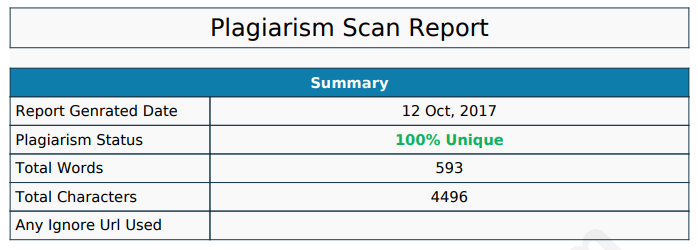
\includegraphics[width=1\textwidth]{figures/plag.PNG}}
\caption{plagiarism}	
\label{plag}
\end{figure}

	
		
	
	
		


\chapter[Sejarah Penentuan Waktu]
{Pengantar\\ Sejarah Penentuan Waktu}
% Kelompok Penentuan Waktu
% Muhammad Nur Ikhsan (1154087)
% Wahyu Maruti Adjie (1154034)
% Ilman Mubarik 	(1154114)
% Emy Safitri		(1154102)
% Andi Ikram Maulana	(1154065)

\section{Sejarah Waktu}
\paragraph{Sejarah Penentuan Waktu diurutkan secara kronlogis dalam sebuah tabel skala waktu geologi 
yang dapat dibagi menjadi beberapa interval sesuai analisis stratigrafi. 
Terdapat 4 garis waktu yang ada, garis waktu yang pertama menunjukkan waktu dari masa-
terbentuknya Bumi sampai waktu sekarang\cite{suryasejarah}. 
Skala waktu kedua menunjukkan eon terbaru dengan skala yang diperluas.} 

\paragraph{Skala waktu kedua, ketiga, dan keempat merupakan sub bagian 
dari skala waktu sebelumnya yang ditunjukkan oleh tanda bintang. 
Alasan lain untuk memperluas skala waktu adalah HOLOSEN (jangka waktu) terakhir 
terlalu kecil untuk dapat ditampilkan dengan jelas
pada skala waktu ketiga disebelah kanan. Gambar \ref{sejarahpenentuan} skala waktu}

\begin{figure}{ht}
\centerline{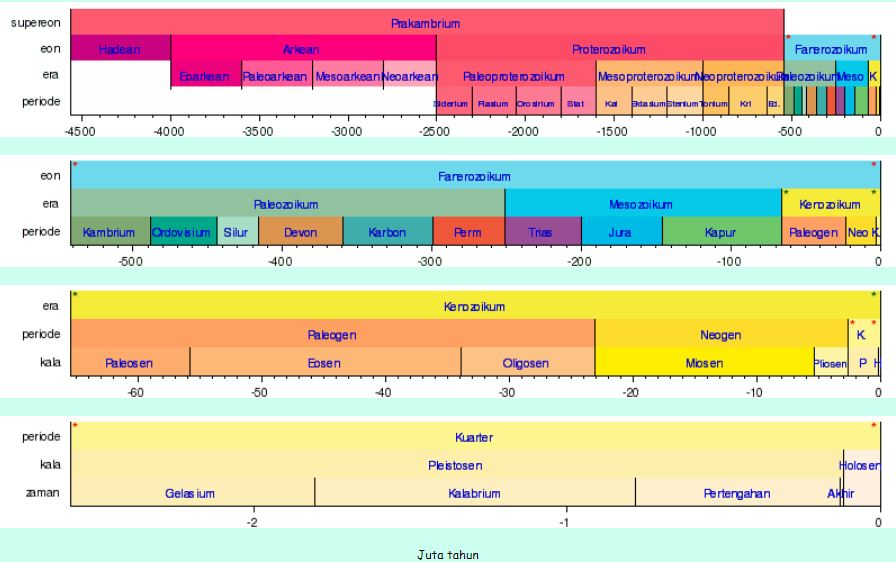
\includegraphics[width=1\textwidth]{figures/sejarahpenentuan.JPG}}
\caption{gambar skala waktu yang ditetapkan.}
\label{sejarahpenentuan}
\end{figure}

\section{Penentuan Waktu}
\paragraph{Pada pembahasan diatas, kita telah membahas tentang sejarah waktu, dan skala waktu. 
Dari penjelasan tersebut, maka dibuatlah suatu pergerakan rotasi bumi. 
Gerakan ini disebut gerakan semu Matahari yang digunakan dalam penentuan waktu (jam).}

\subsection{Hari Matahari}
 \paragraph{Menurut artikel dari rachman planet mengemukakan bahwa satu hari matahari ditentukan
 oleh selang waktu antara dua kulminasi \cite{rachmanplanet}. Kulminasi Atas disebut tengah hari (pukul 12.00)
 dan Kulminasi Bawah adalah saat tengah malam (pukul 24.00 atau pukul 00.00). 
 Dalam kegiatan kita sehari-hari, satu hari matahari adalah waktu yang diperlukan
 Matahari bergerak semu mengelilingi Bumi, terhitung mulai titik Kulminasi Atasnya
 hingga kembali lagi ke titik Kulminasi Atasnya lagi. Dari hasil pengamatan Simamora, ternyata 
 panjang hari matahari (semu) selama setahun berbeda-beda (tidak konstan), 
 hal ini disebabkan:
 
 1)	Bentuk lintasan revolusi Bumi adalah elips.
 Dalam perputaran Bumi mengelilingi Matahari membuat lintasan berbentuk elips 
 sehingga waktu lintasan mengelilingi Matahari (perihelium) 
 pergerakannya cepat dan pada waktu lintasan terjauh 
 dengan Matahari (aphelium) pergeserannya pada ekliptika lambat. 
 Dengan adanya kecepatan gerak Bumi mengelilingi matahari (revolusi)
 tidak sama dengan rotasi bumi tetap, maka terjadilah pergeseran semu
 pada ekliptika tidak seragam, akibatnya saat Matahari mencapai 
 kulminasinya tidak sama. Artinya panjang hari pada hari matahari 
 setiap harinya tidak sama.
 
 2)	Inklinasi ekliptika pada ekuator langit
 Oleh sebab perputaran Bumi pada sumbunya (rotasi) miring maka kedudukan
 bidang ekuator langit dengan bidang ekliptika membentuk sudut 23,50 .
 Akibat dari rotasi bumi itu, sepanjang tahun Matahari seolah-olah bergeser ke arah
 Utara atau ke arah Selatan. Enam bulan berada di belahan Utara dan 
 enam bulan di belahan bumi Selatan. Gerakan tersebut menyebabkan 
 terjadi perbedaan panjang hari terutama pada lintang geografis sedang
 atau tinggi, baik di belahan Bumi Utara atau belahan Bumi Selatan.}
 
\subsection{Hari Bintang}
\paragraph{Hari Bintang adalah selang waktu yang diperlukan sebuah Bintang untuk berkulminasi 
 pada tempat yang sama pada saat berikutnya dalam meridian langit yang 
 sama dari suatu tempat. Satu hari bintang (sehari semalam bintang) adalah 
 waktu yang diperlukan sebuah bintang (lebih umum disebut titik Aries) bergerak semu
 mengelilingi Bumi mulai dari titik Kulminasi Atasnya sampai ke titik Kulminasi Atasnya 
 lagi. Hari Matahari lamanya 24 jam sedangkan hari Bintang adalah 23 jam 56 menit. 
 Jadi perbedaan antara hari Matahari dan  hari Bintang adalah 1/365 x 24 jam atau 
 1/365 x 1440 menit yaitu 3 menit 56 detik  dibulatkan menjadi 4 menit. 
 Jadi pada hari berikutnya Bintang tersebut akan  berkulminasi 4 menit lebih awal.
 Anda dapat menghitung selama 30 hari menjadi  30 x 4 menit yaitu 120 menit atau 2 jam.} 

\paragraph{Jadi setelah 12 bulan (1 tahun) yaitu  12 x 2 jam = 24 jam. Dengan demikian setahun
 kemudian baru Bintang tersebut akan berkulminasi pada jam yang sama. 
 Jadi seolah-olah langit perbintangan berputar kurang lebih 10 setiap hari. 
 Satu tahun Bintang 3600 dibagi 365,25 hari Matahari.}

Sebagai contoh, pada tanggal 23 Maret Bintang Regulus berkulminasi pada pukul 08.00,
 pada tanggal 23 April bintang tersebut berkulminasi pukul 06.00, dan pada tanggal 23 Mei 
 Bintang tersebut berkulminasi pukul 04.00. Dari pendataan tersebut maka: 
 • 1 hari bintang = 1 hari matahari dikurangi 4 menit, 
 • 1 jam bintang = 1 jam matahari dikurangi 1 detik. 
 Dari perhitungan yang dijelaskan maka ada tanggal-tanggal istimewa 
 untuk waktu Bintang dan waktu Matahari, yaitu:
 
	• Tanggal 21 Maret, pukul 00.00 waktu Bintang = pukul 12.00 waktu Matahari,
	• Tanggal 21 Juni, pukul 00.00 waktu Bintang = pukul 06.00 waktu Matahari,
	• Taggal 23 September, pukul 00.00 waktu Bintang = pukul 00.00 waktu Matahari,
	• Tanggal 22 Desember, pukul 00.00 waktu Bintang = pukul 18.00 waktu Matahari.
	
 Jadi hubungan antara Lokal Siderial Times (LST) atau waktu Bintang, 
 dengan Local Civil Times (LCT) dan jumlah hari perbedaan sejak 22,7 September 
 (dibulatkan 23 September) sampai tanggal yang ditentukan adalah:
 LST = LCT + (4.69/70) D. Catatan: 4.69/70 = 4 x 69/70 = 3 menit 56 Detik.	
 
\subsection{Hari Matahari Menengah/Matahari Khayal dan Perata Waktu}
 Dari penjelasan diatas kita, dapat mengetahui bahwa Matahari bukanlah penunjuk 
 waktu yang sangat tepat. Oleh sebab itu, untuk keperluan pembagian waktu yang tepat
 yang kita gunakan sehari-hari, para ahlipun mendasarkan perhitungannya pada Matahari
 khayal. Matahari khayal ini adalah Matahari yang dianggap atau dimisalkan ada, 
 yang kecepatan pergeserannya hampir sama dengan perpindahan Matahari sebenarnya.
 
 Perbedaannya adalah Matahari khayal ini bergeser sepanjang ekuator langit 
 dengan kecepatan pergeseran yang tetap (konstan) atau seragam, hingga panjang satu
 “hari matahari khayal” = panjang rata-rata “hari matahari sebenarnya”. 
 Oleh karena itulah hari matahari khayal disebut pula hari matahari menengah.
 
  Pada saat matahari menengah inilah didasarkan pembagian waktu pada jam yang kita gunakan sehari-hari, karena setiap hari matahari menengah panjangnya tetap sama sepanjang tahun.

	1 hari matahari menengah = 24 jam waktu matahari menengah 
	1 jam waktu matahri menengah = 60 menit waktu matahari menengah
	1 menit waktu matahari menegah = 60 detik waktu matahari menengah
	
	Bandingkan
	1 hari matahari menengah = 24 jam waktu matahari menengah (jam kita)
							 = 24 jam 4 menit waktu bintang (24 jam 3menit 57detik)
	1 hari bintang		     = 24 jam waktu bintang
							 = 23 jam 6menit waktu matahari menengah 
							  (tepatnya 23 jam 56 menit 4 detik)
								  
Waktu matahari menengah dimulai ketika matahari menengah terdapat pada titik
 Kulminasi Bawahya (pukul 00.00 waktu matahari menengah), cara membedakannya mulai 
 dari waktu bintang yang dimulai pada saat titik Aries berada
 pada titik Kulminasi Atasnya (pukul 00.00 waktu bintang).


Hari Matahari Menengah kadang-kadang lebih sedikit pendek dari Hari Matahari 
 Sebenarnya tetapi terkadang lebih panjang.   Perbedaan maksimal hanyalah 
 sampai kira-kira seperempat jam. Perbedaan waktu ini disebut Perata Waktu, 
 dengan rumus:
				Perata Waktu = Hari Matahari Menengah – Hari Matahari Sebenarnya
							(Simamora,P., 1975: 72)
								
Perata waktu ini dinyatakan dengan tanda positif (+) jika 
 matahari menengah mendahului matahari sebenarnya dan tanda negatif (-)
 jika terjadi sebaliknya. Perata waktu terbesar terjadi pada 11 Februari,
 yaitu + 14 menit dan 2 November, yaitu – 16 menit. Dalam satu tahun terjadi 
 empat kali panjang hari matahari menengah sama dengan pajang hari matahari sebenarnya,
 yaitu 15 April, 14 Juni, 1 September, dan 24 Desember. Pada hari-hari ini perata 
 waktunya adalah 0 menit.  Untuk lebih jelasnya perhatikan gambar \ref{sejarahwaktu_Capture} di bawah ini								
	
	\begin{figure}{ht}
	\centerline{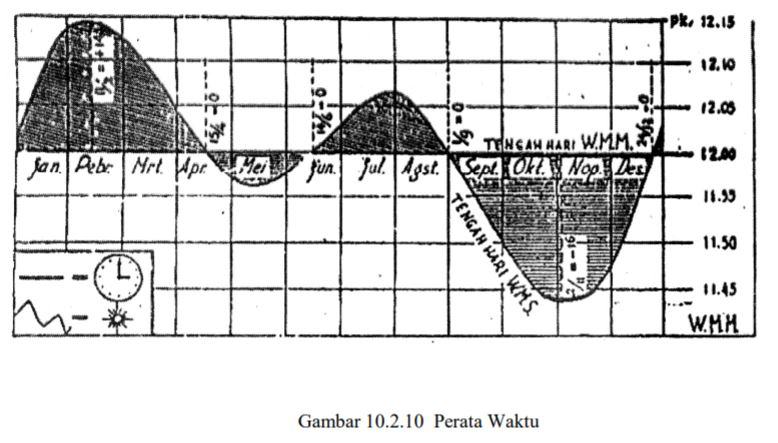
\includegraphics[width=1\textwidth]{figures/sejarahwaktu_Capture.JPG}}
	\caption{gambar Perata Waktu.}
	\label{sejarahwaktu_Capture}
	\end{figure}

 Dari gambar \ref{sejarahwaktu_Capture} kita dapat mengetahui pula bahwa sekitar bulan Januari, Februari
 Maret, Juli, dan Agustus matahari sebenernya lebih lambat sampai titik Kulminasi atasnya,
 sehingga sore lebih lama terangnya.
 
	Contoh: Pada tanggal 2 November jam ditangan kita (waktu matahari menengah) 
	menunjukkan pukul 12.00, tetapi Matahari di langit masih belum tiba di titik Kulminasi 
	Atasnya, baru -16 menit kemudian hal itu terjadi, yaitu pada pukul 11.44 waktu matahari 
	menengah. Sebaliknya, pada bulan Oktober, November, dan Desember matahari menengah 
	lebih lambat daripada matahari sebenarnya. Pagi hari Matahari telah terbit sedangkan 
	jam kita masih menunjukkan kurang dari pukul 06.00. Pada sore harinya pukul 06.00 sudah
	gelap. Hal ini terjadi pada sekitar khatulistiwa (termasuk di Indonesia), 
	di daerah-daerah sedang dan kutub tentunya berbeda.
	
\subsection{Greenwhich Mean Time(GMT)}
Greenwich Mean Time (GMT) adalah tempat yang menjadi
 patokan waktu dunia berada. Jika ditentukan dengan penentuan waktu GMT lebih mudah kita
 dapat menghitung waktu-waktu di seluruh permukaan Bumi. Bagi daerah yang
 berada di belahan barat (meridian barat) waktu setempat adalah waktu GMT
 ditambah dengan hasil kali perbedaan meridian dengan 4 menit sedangkan daerah
 yang berada di belahan timur (meridian timur) waktu setempat adalah waktu GMT
 dikurangi dengan hasil kali antara selisih meridian dengan 4menit. 
 cara perumusannya dengan menggunakan:
					LMT = GMT +(M.4)
			(Dardjosoemartp, dkk.,1991: 445)
			
	LMT = Local Mean Time / Waktu Setempat 
GMT = Greenwich Mean Time / waktu GMT
 + = + bila di BB dan – bila di BT 
(M.4) = meridian (bujur) x 4 menit

\section{Waktu Standar}
\paragraph{Tempat-tempat yang terletak pada garis meridian yang sama, mempunyai waktu yang sama.
 Jika demikian, seluruh permukaan Bumi terdapat 360 waktu yang bedanya 4 menit.
 Hal ini tentu rumit dalam kehidupan sehari-hari. Oleh sebab itu, disepakatilah untuk
 membagi permukaan Bumi atas 24 daerah waktu saja yang disebut waktu standar.}
 
 \paragraph{Waktu standar disebut juga Zone Time, yaitu waktu yang ditetapkan setiap 
 selisih 150 adalah 60 menit (1 jam) dengan lingkup daerah yang berada pada 00 – 150
 atau 150 – 300 , dan seterusnya baik di Bujur Timur maupun Bujur Barat.}
 
 Kongres Internasional memutuskan tentang garis-garis meridian (International Meridian Conferense) 
 di Washington menetapkan waktu standar dunia yang dibagi menjadi 24 daerah berdasarkan
 perbedaan meridian 150 . Setiap daerah mempunyai selisih waktu 1 jam.
 Akan tetapi berdasarkan pembagian wilayah kepemerintahan atau kontinen (pulau/benua)
 maka ada sedikit pergeseran. Batas yang terdapat pada 1800 BT dan 1800 BB berupa garis
 yang berkelok-kelok. Perhatikan gambar \ref{sejarahwaktu_Capture1} di bawah ini:
 
 \begin{figure}{ht}
 \centerline{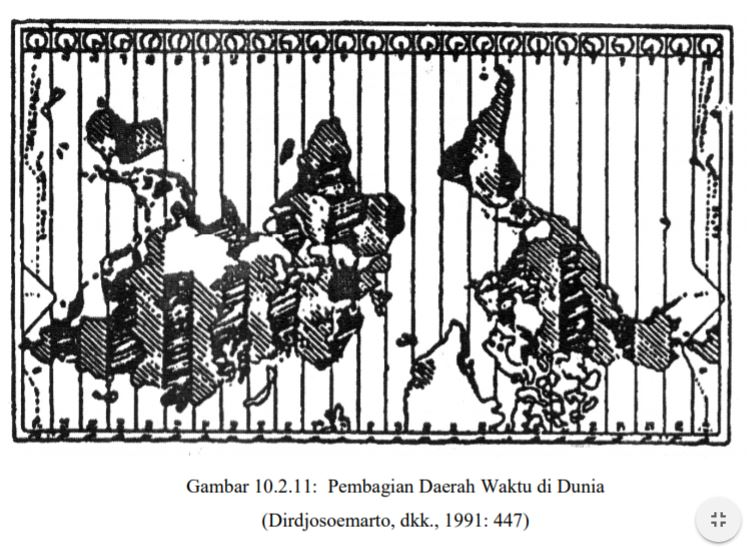
\includegraphics[width=1\textwidth]{figures/sejarahwaktu_Capture1.JPG}}
 \caption{gambar Pembagian Daerah Waktu di Dunia.}
 \label{sejarahwaktu_Capture1}
 \end{figure}
 
 
Setiap negara mempunyai pembagian daerah waktu yang berbeda-beda karena letak pada meridianya berbeda. 
 Indonesia terletak antara 950 BT – 1410 BT. Oleh karena Indonesia mempuyai rentang meridian 1410 – 950 = 460 , 
 maka Indonesia di bagi menjadi 3 daerah waktu, yakni Waktu Indonesia bagian Barat (WIB),
 u Indonesia bagian Tengan (WITA), dan Waktu Indonesia bagian Timur (WIT) dengan selisih
 satu jam. Untuk lebih jelasnya,  perhatikan gambar \ref{sejarahwaktu_Capture2} di bawah.
 
 \begin{figure}{ht}
 \centerline{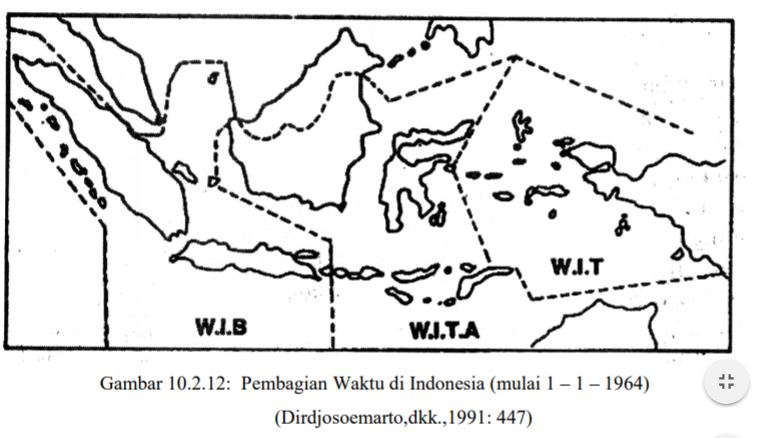
\includegraphics[width=1\textwidth]{figures/sejarahwaktu_Capture2.JPG}}
 \caption{gambar Pembagian Waktu di Indonesia.}
 \label{sejarahwaktu_Capture2}
 \end{figure}
 

Indonesia mempunyai tiga meridian standar, yaitu meridian 1050 BT untuk daerah WIB, 
 1200 BT untuk daerah WITA, dan 1350 untuk WIT .  Dengan demikian waktu lokalnya (LMT) 
 masing-masing adalah waktu Greenwich 
 ditambah 105/15 untuk WIB, 120/15 untuk WITA, dan 135/15 untuk WIT .
 Jika waktu GMT pukul 12.00, maka: WIB = 12.00 + (105/15 = 7) yaitu pukul 19.00,
 WITA = 12.00 + (120/15 = 8) yaitu pukul 20.00, 
 dan WIT = 12.00 + (135/15 =9) yaitu pukul 21.00 (Hidayat,B.,1978: 42).
 \end{document}


\chapter[Sejarah Penanggalan]
{Pengantar\\ Sejarah  Penanggalan}
%Define sejarah penanggalan,bulan dan tahun
%kelompok 4 D4 TI-2D
%Ayu Permata Sari        1154022
%Librantara Erlangga     1154071
%Martin Luter Zega       1154120
%Putri Aulia Ramadhanie  1154096
%Ryan Hafizh Herdiana    1154067
%Copyright (c) 2017 Copyright Holder All Rights Reserved.


\section{Sejarah penanggalan}
  Penanggalan merupakan salah satu sebuah mahakarya yang bisa ditemukan oleh umat manusia. Manusia mempelajari dan memanfaatkan alam [Matahari,Bulan dan Bintang] untuk menghitung pergantian tanggal,bulan dan juga tahun.
umumnya penanggalan digunakan untuk mengetahui waktu yang telah dilewati oleh umat manusia. Adanya sistem penanggalan ini membuat manusia dapat mengingat seluruh kejadian dan pristiwa yang terjadi di dunia ini.
Menurut artikel dari setyanto berdasarkan benda langit yang digunakan sebagai dasar perhitungan sistem penanggalan dapat dikategorikan menjadi 3 kelompok yaitu:\cite{setyanto2015kriteria}

  \subsection{Solar calendar/Kalender Surya}
    Kalender surya menggunakan pergerakan bumi mengelilingi matahari sebagai acuannya.Sistem kalender surya ini biasa digunakan oleh orang-orang eropa. Beberapa contoh kalender yang menggunakan sistem ini yaitu:

    \subsubsection{Julian calendar/Kalender Julian}
      Kalender julian merupakan contoh kalender yang menerapkan sistem surya menurut artikel dari rachmanplanet\cite{rachmanplanet}.Kalender ini telah digunakan bahkan 45 tahun sebelum masehi.
    Awalnya ketika Julius Caesar memimpin pemerintahn romawi terjadi kekacauan  pada perhitungan kalender yang menyebabkan Julis Caesar saat itu mengakhirinya dengan membuat perhitungan kalender sendiri dengan ketentuan:
      1)Satu tahun ditetapkan 565,25 Hari
      2)Tahun biasa, yaitu tiga tahun berturut-turut yang harinya berjumlah 365 Hari
      3)Tahun Kabisat, yaitu tahun keempat ditambah satu hari menjadi 366 Hari.Tambahannya dilakukan pada bulan februari yang jika pada tahun biasa 28 hari pada tahun kabisat ini menjadi 29 hari
      4)Titik permulaan musim semi/bunga ditetapkan pada tanggal 24 Maret
      5)Permulaan tahun ditetapkan pada tanggal 1 Januari (Sebelumnya awal tahun ditetapkan pada tanggal 24 Maret)
    Meskipun kalender julian sudah sangat baik namun ternyata masih terdapat cacat pada kalender tersebut.
    Sebelum orang romawi menggunakan kalender julius caesar, orang romawi sudah menggunakan nama-nama bulan seperti:
    \begin{enumerate}
      \item  Martius     = 31 hari
      \item  Aprilis     = 29 hari
      \item  Majus       = 31 hari
      \item  Junius      = 29 hari
      \item  Quintilis   = 31 hari
      \item  Sextilis    = 29 hari
      \item  September   = 29 hari
      \item  October     = 31 hari
      \item  November    = 29 hari
      \item  Dcember     = 29 hari
      \item  Januarius   = 29 hari
      \item  Februarius  = 28 hari
    \end{enumerate} 

    \subsubsection{Gregorian calendar/Kalender Gregorius}
      Pada tahun 1582 Masehi Paus Gregorius menyaksikan musim semi/bunga pada tanggal 11 maret,bukan lagi pada tanggal 24 maret seperti pada kalender julian.Kemudian paus gregorius memperbaiknya dengan cara:
      1)Musim semi/bunga ditetapkan pada tanggal 21 Maret
      2)Tahun biasa menjadi 365 hari dan tahun kabisat menjadi 566 hari
      Kalender gregorius lebih dikenal dengan nama kalender masehi yang jumlah hari pada setiap bulan dan pentapan awal tahun seperti yang digunakan kalender umumnya saat ini.Kalender masehi dimulai dari tanggal 1 januari
      tahun 1, pukul 00.00.Penamaan bulan pada kalender gregorius yang digunakan hingga sekarang:
      \begin{enumerate}
        \item  January   = 31 hari
        \item  February  = 28/29 hari
        \item  March     = 31 hari
        \item  April     = 30 hari
        \item  May       = 31 hari
        \item  June      = 30 hari
        \item  July      = 31 hari
        \item  August    = 31 hari
        \item  September = 30 hari
        \item  October  = 31 hari
        \item  November = 30 hari
        \item  December = 31 hari
      \end{enumerate}

  \subsection{lunar calendar/Kalender candra}
    \ref{Kalender_2015}
    \begin{figure}[ht]
    \centerline{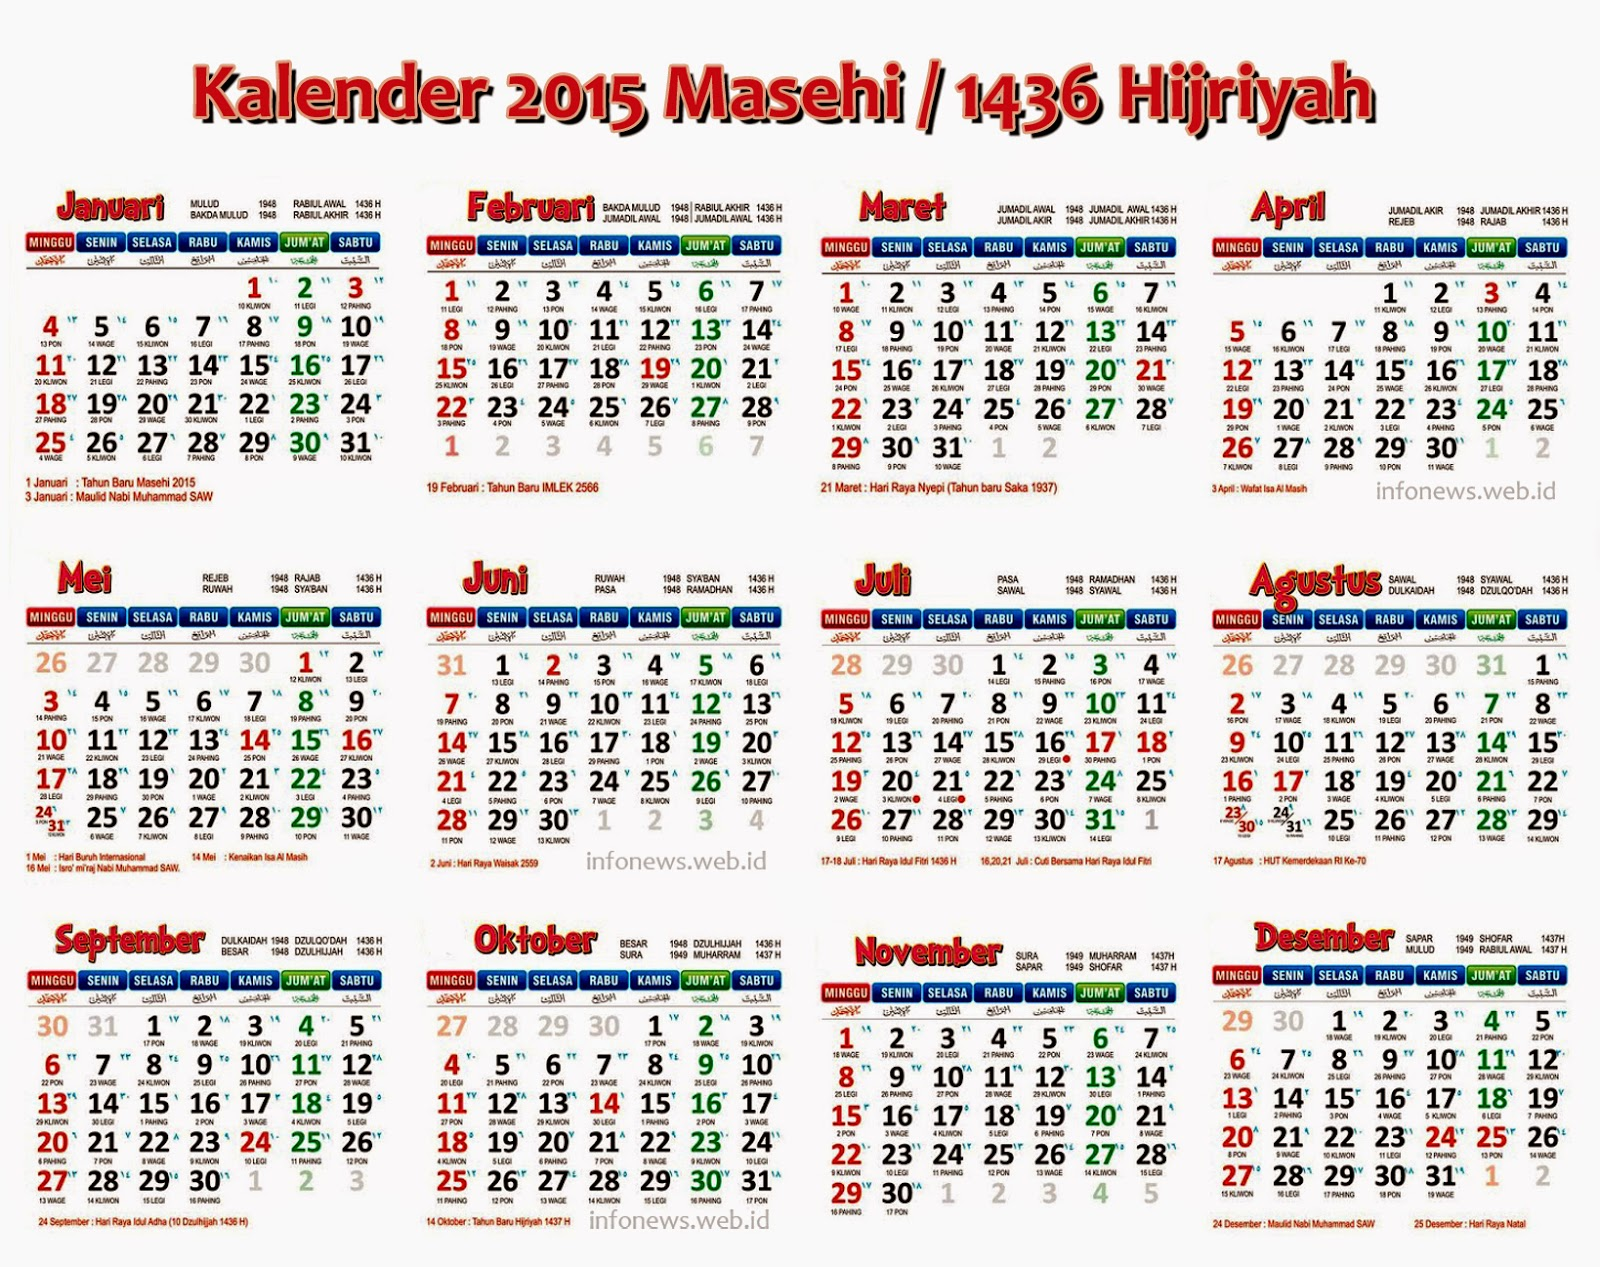
\includegraphics[width=1\textwidth]{figures/Kalender_2015.JPG}}
    \caption{Kalender tahun 2015 Masehi / 1436 Hijriyah.}
    \label{Kalender_2015}
    \end{figure}
    Pembahasan kelender hijriah terkait dengan sistem penanggalan yang berpedoman pada pergerakan Bulan tampak dari Bumi yaitu ketika Matahari dan Bulan yang berada pada posisi bujur astronomi yang sama. Konjungsi merupakan pergerakan pada posisi Bulan dan Matahari yang terlah disepakati sebagai batas penentuan secara astronomis pada kelender Hijriah.
  Bulan yang berkonjungsi searah dengan Matahari akan tampak gelap pada permukaannya ketika dilihat dari Bumi dengan bentuk cahaya sabit kecil. Bulan baru adalah piringan kecil Bulan yang muncul setelah mengalami satu putaran penuh pada fase Bulan mengelilingi Bumi.
  Kemunculan hilal (bulan baru) merupakan penentuan awal bulan dalam Kelender Hijriah di Indonesia, terkhusus pada bulan Ramadhan, Syawal, dan Zulhijah.Kalender merupakan sistem pengorganisasian waktu yang berfungsi sebagai penanda perhitungan dalam jangka panjang. Kelender hijriah termasuk jenis kelender yang penanggalannya berpatokan pada Bulan ketika mengorbit kepada Bumi.
  Perbedaan antara tahun syamsiah dan tahun kamariah yaitu umur hari dalam satu tahun yang 11 hari juga berbeda dalam penentuan awal perhitungan hari. Penanggalan kamariah memiliki perhitungan yang dimulai sejak terbenamnya Matahari dan berakhir ketika Matahari terbenam pada hari esoknya.
  Sistem penanggalan Islam atau kalender hijriah adalah sistem penanggalan yang memiliki dua belas bulan, dimulai sejak Bulan baru hingga penampakan bulan baru berikutnya berkisar selang waktu antara 29 sampai 30 hari. Rovolusi bulan mengililingi bumi memiliki bentuk lintasan yang elips dengan kecepatan tempuh total dalam satu tahun adalah 354 hari 48 menit dan 34 detik.
  Bulan sebagai salah satu komponen penting dalam penanggalan kamariah yakni merupakan satelit tunggal yang dimiliki Bumi. Bulan memiliki 3 pergerakan, diantaranya pergerakan rotasi atau Bulan berputar pada porosnya, revolusi terhadap bumi dan revolusi bersamaan dengan bumi terhadap matahari.

    \subsubsection{Sejarah Kalender Hijriyah}\cite{setyanto2015kriteria}
      Pada saat Sebelum peristiwa haji Wada’ yang dilaksanakan oleh Nabi dan kaum Muslimin, sistem penanggalan masyarakat Arab di Makkah kala itu masih menggunakan konsep penanggalan al-Nasī’. Keberadaan istilah waktu al-Nasī’ tersebut telah mempersulit untuk merunutkan fenomena/peristiwa yang terjadi sebelum haji Wada’.
    Hal ini dikarenakan aturan penggunaan waktu al-Nasī’ tidak berjalan dengan baik. Bangsa Arab dikenal sering memundur dan memajukan kegiatan-kegiatan yang dilakukan pada bulan-bulan Haram sesuai dengan kebutuhannya.4 Hal inilah yang menjadikan penanggalan masyarakat Arab sebelum Haji Wada’ dapat dikatakan tidak konsisten.
    Maksud istilah waktu al-Nasī’ (waktu pengunduran) yaitu diundurnya waktu untuk melaksanakan suatu kegiatan pada waktu tertentu. Salah satunya adalah pengunduran waktu ibadah haji oleh masyarakat Arah ketika itu. Mereka terkadang melaksanakan ibadah haji pada waktunya, terkadang pula pada bulan Muharam, Ṣafar, dan bulan-bulan lainnya di antara dua belas bulan.
    Dampaknya, adalah hal-hal yang mereka yang biasanya dilakukan pada bulan-bulan haram menjadi terabaikan. Hal ini dikarenakan pada saat mereka sedang melaksanakan ibadah haji, mereka bertemu dengan pembunuh ayah mereka, atau bertemu dengan pembunuh sanak saudara mereka, yang menyebabkan mereka membalas dendam pada waktu tersebut.
    Padahal Allah telah menerangkan bahwa melakukan amalan-amalan saleh pada bulan-bulan tersebut merupakan sebesar-besarnya pahala. Sebaliknya, perbuatan zalim yang dilakukan pada saat itu seburuk-buruknya kesalahan, bahkan menambah kekafiran.
    Namun demikian, konsep al-Nasī’ dimaksudkan untuk menyesuaikan fase Bulan dengan perubahan musim yang diakibatkan oleh posisi dan gerak Matahari di Jazirah Arab.Sehingga dapat dikatakan penanggalan masyarakat Arab ketika itu termasuk menggunakan sistem Penanggalan Matahari-Bulan (Kala Surya-Chandra).
    Meski demikian, Nabi Muhammad beserta umat Islam kala itu mengikuti kalender yang sedang berjalan. Sehingga dapat dikatakan seluruh hidup Nabi Muhammad berpuasa dalam sistem penanggalan yang ditetapkan oleh bangsa Quraisy. Nabi tidak membuat sistem penanggalannya sendiri.Turunnya QS.
    al-Taubah [9]: 36-37, yang melarang penggunaan yaum al-Nasi’ (waktu pengunduran) telah mengubah sistem penanggalan masyarakat Arab dari sistem Lunisolar Calendar menjadi sistem Lunar Calender. hal Inilah yang menjadi awal mula atau kelahiran sistem penanggalan Islam yang berbasis pada pergerakan Bulan dalam mengelilingi Bumi.
    Hingga saat ini belum diketahui dengan baik bagaimana praktek penanggalan Islam pada zaman sahabat. Namun, diyakini penanggalan Islam pada masa itu didasarkan pada kesaksian ru’yat al-hilāl. Adapun proses bagaimana praktek penanggalan Hijriyah sejak berubahnya sistem penanggalan tersebut pada dasarnya dapat ditelusuri melalui sejarah, sebagaimana yang telah dilakukan oleh Saleh al-Saab dari King Abdul’aziz City for Science and Technology (KACST), Riyadh.
    Praktek penanggalan Islam kemudian disempurnakan melalui konsep penanggalan yang dirumuskan pada zaman Umar bin Khaṭṭab. Melalui sidang para sahabat rasulullah, ditetapkanlah perhitungan tahun dalam penanggalan kekhalifahan, dimulai sejak hijrahnya Nabi Muhammad dari Mekkah ke Madinah.
    Penetapan tahun hijrahnya Nabi sebagai tahun pertama tersebut merupakan usulan dari Sahabat ‘Ali bin Abī Ṭālib.11 Oleh karena itu, penanggalan kekhalifahan Islam dikenal sebagai penanggalan Hijriyah, dengan bulan Muharam sebagai bulan pertama dalam penanggalan tersebut. Hal tersebutlah yang telah umum berlaku di masyarakat Arab ketika itu.
    Sama halnya dengan penanggalan Masehi yang digunakan saat ini, penanggalan Hijriyah pun pada zaman sahabat ditetapkan berdasarkan perhitungan matematis. Jumlah hari yang digunakan senantiasa tetap setiap bulannya. Meskipun demikian, hal-hal yang terkait dengan pelaksanaan ibadah kaum Muslimin kala itu tetap mengikuti ketentuan yang telah diajarkan oleh Nabi Muhammad.
    Oleh karenanya, penanggalan pada kalender Hijriyah yang telah ditetapkan merupakan penanggalan Administrasi Negara.Seiring dengan perkembangan pemahaman dan pengetahuan, saat ini fungsi penanggalan Hijriyah sebagai penanggalan sosial menjadi satu kesatuan dengan fungsinya sebagai penanggalan ibadah. Hal inilah yang dilihat secara subyektif sebagai kisruh sistem penanggalan Hijriyah.
    Maka dari itu, untuk mengurai permasalahan pada tahap awal adalah dengan melepaskan fungsi ibadah dari sistem penanggalan Hijriyah.Namun, aturan ibadah tetap menjadi acuan dalam penyusunan kalender Hijriyah, sebagaimana yang telah dipraktekkan oleh sahabat. Dalam beribadah terdapat kesepakatan pada proses pencapaian kesatuan dalam beribadah yaitu dapat diawali dengan menyepakati penggunaan kalender tunggal yang digunakan bersama, sedangkan pelaksanaan ibadah dikembalikan kepada masing-masing.Berikut adalah nama bulan dan hari pada kalender hijriyah berdasarkan pada hisab urfi:
    \begin{enumerate}
        \item Muharram      = 30 hari
        \item Shafar        = 29 hari
        \item Rabiul Awwal  = 30 hari
        \item Rabiul Akhir  = 29 hari
        \item Jumadil Awwal = 30 hari
        \item Jumadil Akhir = 29 hari
        \item Rajab         = 30 hari
        \item Shaban        = 29 hari
        \item Ramadhan      = 30 hari
        \item Syawal        = 29 hari
        \item Dzulka'idah   = 30 hari
        \item Dzhulhijjah   = 29/30 hari
    \end{enumerate}

  \subsection{lunisolar calendar/kalender suryacandra}
      Menurut wicaksono dalam artikelnya Lunisolar kalender merupakan sistem kalender candra yang disesuaikan dengan matahari \cite{wicaksono2008ta}.Karena kalender candra dalam 1 tahun mempunyai 11 hari lebih cepat dari kalender surya, maka dalam kalender suryacandra memiliki bulan interkalasi(bulan tambahan/bulan ke -13)setiap 3 tahun, agar kembali seusai dengan perjalanan matahari.
    beberapa contoh kalender yang mengacu pada sistem suryacandra adalah kalender imlek/cina,saka,dan budhha. Semua kalender tersebut tidak ada yang sempurna ,karena jumlah hari dalam satu tahun itu tidak bulat,dan untuk memperkecil error itu maka dibuat kesepakatan sehari lebih panjang atau terdapat bulan tambahan dalam kalender cina pada tahun kabisat\cite{wicaksono2008ta}.
    Pada kalender surya, pergantian hari terjadi tengah malam dan awal setiap bulan (tanggal 1) yang tidak tergantung pada posisi bulan dan pada kalender candra dan suryacandra pergantian hari terjadi ketika matahari terbenam dan awal setiap bulan adalah saat konjungsi(imlek,sakka,budhha) atau dalam hijriyah saat munculnya hilal.




\chapter[Bangun Ruang]
{Pengantar\\ Bangun Ruang}
%kelompok 2
%Achmad Fatahillah(1154004)
%Ilga Anne Tri J.S(1154045)
%Maulyanda(1154008)
%Mefi Frinkazela Nikica(1154073)
%Simon Sorba Manangi(1154019)
	
\section{Bangun Ruang}
Bangun ruang merupakan suatu bagian ruang yang dibatasi oleh himpunan titik-titik yang terdapat pada seluruh permukaan bangun tersebut. 
Permukaan bangun tersebut disebut sisi. Bangun ruang memiliki tiga unsur, yaitu 
panjang : merupakan suatu dimensi dalam benda yang menunjukkan sebuah jarak antar ujung satu ke ujung lainnya.
lebar   : merupakan lintasan dalam sebuah bidang.
tinggi  : merupakan ukuran sebuah objek yang diukur secara vertikal.
Bangun ruang memiliki volume. Rumus volume umum pada bangun ruang adalah panjang(p) x lebar(l) x tinggi(t).
Tujuan menghitung volume adalah untuk menghitung berapa banyak ruang yang dapat diisi datau ditempati pada suatu objek.

Sisi bangun ruang adalah suatu himpunan pada titik-titik yang terdapat pada permukaan atau yang membatasi suatu bangun ruang tersebut \cite{umami2013eksperimentasi}

Dalam memilih model untuk permukaan atau sisi, dapat karena kedudukan semua unsur bangun ruang dapat diamati untuk dialihkan dalam gambar\cite{suharjana2008mengenal}. 
Ada beberapa contoh benda yang mewakili gambar bangun ruang\ref{contohbangun}.
\begin{figure}[ht]
    \centerline{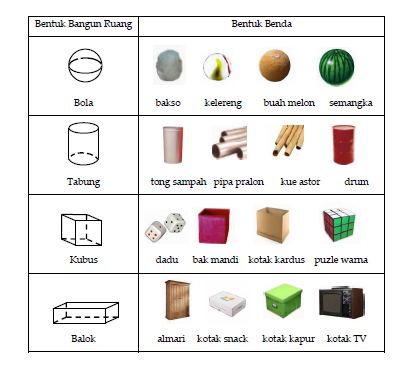
\includegraphics[width=1\textwidth]{figures/contohbangun.png}}
    \caption{beberapa kumpulan gambar yang termasuk dalam bangun ruang}
    \label{contohbangun}
    \end{figure}
 
Bangun ruang sering  disebut bangun 3 dimensi karena memiliki 3 komponen utama sebagai berikut.
1.Sisi  merupakan bidang pada bangun ini memiliki ruang yang membatasi antara bangun ruang dengan ruangansekitarnya 
2.Rusuk merupakan pertemuan antar dua sisi yang berupa ruas garis pada bangun.
3.Titik sudut merupakan titik hasil pertemuan rusuk yang berjumlah tiga atau lebih

Unsur-unsur Bangun Ruang Sisi,rusuk,dantitiksudut. Sebagai mengingatkan bahwa setiap model bangun ruang pasti memiliki sisi, rusuk, dan titiksudut , kecuali bola, tabung,dankerucut.
Bangun ruang, limas, prisma, dan sisi, rusuk, titiksudut serta dikembangkan pada diagonalsisi,diagonalruang, dangaris-garis sejajar.
menggunakan model bangun ruang yang transparan  melihat sisi bangun ruang tersebut, model transparan, bangun ruang dengan model transparan ini juga dapat untuk menggambar bangun ruang, karena semua unsur bangun ruang dapat diamati untuk dialihkan dalam gambar. Setelah mengamati, 
menelusuri, dan memahami unsur-unsur bangun ruang tersebut.

Jenis-Jenis Bangun Ruang yang umum dikenal adalah:
1.  kubus merupakan bangun ruang yang dibatasi oleh enam buah bidang sisi berbentuk persegi dengan ukuran yang sama.
2.balok yaitu bangun ruang dengan dibatasi dengan enam bidang sisi yang memiliki bentuk persegi panjang yang setiap sepasang-sepasang sejajar dan sama ukurannya.
3.prisma yaitu adalah sebuah bangun ruang yang diberikan batas oleh dua buah daerah segitiga yang sejajar sehingga tiga daerah persegi panjang tersebut yang saling berpotongan menurut garis-garis yang sejajar.
4.limas merupakan bangun ruang yang dibatasi leh sebuah daerah segiempat dan empat daerah segitiga yang mempunyai satu titik sudut persekutuan.
5.kerucut merupakan bangun ruang yang dibatasi oleh sebuah bidang lengkung yang simetris terhadap porosnya yang melalui titik pusat lingkaran tersebut.
6.tabung merupakan bangun ruang yang setiap sisinya dibatasin dengan dua bidang lingkaran yang sama-sama sejajar dan sama-sama ukurannya dan satu buah bidang 
     yang memiliki jarak sama jauhnya ke arah poros dan sisi yang simetris ke arah porosnye itu akan memotong dua daerah bidang lingkaran tepat di kedua lingkaran itu .
7.Bola
Jenis-Jenis Bangun Ruang yang umum dikenal adalah dan di dalam kehidupan sehari hari:
1.   Kubus    : dadu, rubik
2.   Balok    : lemari, tv
3.   Prisma    : atap rumah, tenda pramuka
4.   Limas    : piramida, monas
5.   Kerucut: nasi tumppeng yang berbentuk kerucut
6.   Tabung    : minuman kaleng, gas elpiji
7.   Bola    : bola basket, bola tenis

Dalam pembelajaran bangun ruang dan unsur-unsurnya maka harus DIPERKENALKAN model-model bangun ruang, misalnya model kubus, balok, prisma, limas, tabung, kerucut, dan bola. apabila diambil contoh-contoh dari bendabenda yang dapat ditemukan dalam kehidupan sehari-hari, misalnya kaleng roti untuk menunjukkan tabung, tumpeng untuk menunjukkan kerucut dan seterusnya. Yang tidak transparan, transparan dan kerangka. Hal tersebut akan lebih memudahkan dalam pemahamanbangun ruang dan unsur unsurnya, menentukan sifat sifat bangun ruang, serta dapat menterjemahkan gambar dalam bangun ruang dans ebaliknya.
Contoh di bidang bangun ruang yaitu dalam bidang geometri  materi matematika bentuk bangun datar 2D maupun bangun ruang 3D. 
Manfaat yang dapat diperoleh dari penelitian memberikan gambaran 3D dari pemodelan bangun geometri halnya alat perga dalam membangun siswa dalam mempelajari bentuk bangun geometri.
Bangun ruang dalam bentuk geometris yang terdiri atas tiga dimensi( panjang lebar dan tinggi) bangun ruang yang di bahas di dalam geometri antara lain :
1.    Kubus
2.    Balok 
3.    Prisma
4.    Limas
5.    Tabung
6.    Kerucut
7.    Bola

Kebutuhan di bangun ruang dapat disimpulkan bahwa diperlukan 
1.    Pengertian dan ciri-ciri berapa bangun datar dan bangunan ruangan.
2.    Data rumus luas bangun datar.
3.    Data rumus volum bangun datar dan bangun ruang.

Kebutuhan disini sudah diperoleh dari buku matematika sekolah dasar.

\subsection{Bola} 

\begin{figure}[ht]
    \centering
	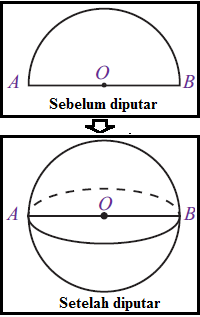
\includegraphics[width=0.5\textwidth]{figures/bola1.png}
    \caption{contoh bola}
    \label{bola1}
\end{figure}

Dalam bangun ruang, bola adalah bangun ruang tiga dimensi yang dibentuk sehingga tak terhingga lingkaran yang berjari-jari sama panjangnya dan berpusat pada satu titik yang sama. Bola merupakan bangun ruang sisi lengkung yang dibatasi oleh satu bidang lengkung.
contoh bangun ruang bola dalam kehidupan sehari-hari adalah dalam sebuah olah raga sepak bola, basket, kasti, bowling, dan sebagai nya. bola dapat menggelinding dan dapat memantul dengan sempurna, karena tidak adanya sudut pada bola. 
Bentuk bumi pun seperti bola, terlihat pada sebuah dokumentasi dari pesawat ruang angkasa, maupun dalam hal perjalan lurus, pasti akan kembali lagi ketempat kita memulai perjalanan.
Bola dapat dibentuk dari bangun setengah lingkaran yang diputar sejauh 360° pada garis tengahnya. 
Pada gambar  \ref{bola1} merupakan setengah lingkaran dengan diameter AB  tersebut dan dapat diputar satu putaran dengan diameter sebagai suatu sumbu putar maka akan tampak gambar seperti di bawahnya yang disebut bangun ruang.


Bola merupakan bangun ruang sisi lengkung (BRSL) yang terjadi dari tumpukan empat buah lingkaran \ref{sisilengkung}.
\begin{figure}[ht]
    \centering
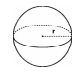
\includegraphics[width=0.25\textwidth]{figures/sisilengkung.png}
    \caption{contoh sisi lengkung}
    \label{sisilengkung}
    \end{figure} 
Keempat lingkaran ini dinamakan kulit bola. Kulit bola berada pada sisi luar bola atau mengelilingi bola \cite{nurfarikhin2010hubungan}.

Rumus bola:

a) Luas permukaan
 \begin{equation}
     L = 4 \pi r^2 \,
\end{equation}
b) Volume
\begin{equation}
     V = \frac{4}{3}\pi r^3
\end{equation}
\subsubsection{Sifat-sifat pada bola} 
a) Memiliki 1 sisi yang berbentuk bidang lengkung (selimut bola) 
b) Tidak memiliki rusuk 
c) Tidak memiliki titik sudut
 
Adapun unsur-unsur bangun ruang bola yang terdapat pada gambar \ref{unsurbola} sebagai berikut.
\begin{figure}[ht]
    \centerline{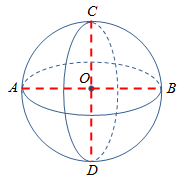
\includegraphics[width=1\textwidth]{figures/unsurbola.png}}
    \caption{contoh usur bola}
    \label{unsurbola}
    \end{figure}
1) Titik pada titik O dinamakan titik pusat bola.
2) Ruas garis pada OA disebut sebagai jari-jari pada bola. Sebutkan jari-jari pada bola lainnya.
3) Ruas garis pada CD diberi nama sebagai diameter pada bola. Jika kita amati, ruas pada garis AB tersebut merupakan diameter bola. AB dapat pula disebut sebagai tinggi bola.
4) Sisi bola merupakan kumpulan titik - titik yang mempunyai jarak yang sama terhadap titik O. Sisi tersebut dinamakan selimutatau kulit bola.
5) Ruas garis ACB dinamakan tali busur bola.
6) Ruas-ruas pada garis selimut bola yaitu ACBDA dinamakan garis pelukis bola.

\subsubsection{Konsep luas permukaan Bola}
Penentuan luas sisis (permukaan) bola dapat kita lakukan dengan sebuah percobaan archimedes, yaitu:
Sebuah bola menempati sebuah tabung yang memiliki diameter dan tinggi tabung sama tepat dengan 
yang dimiliki oleh diameter bola, maka luas bola itu sama dengan luas selimut tabung \ref{bolatabung}.
\begin{figure}[ht]
    \centerline{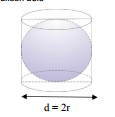
\includegraphics[width=1\textwidth]{figures/bolatabung.png}}
    \caption{sebuah bola yang terdapat dalam tabung, untuk mengukur luar permukaan tabung}
    \label{bolatabung}
    \end{figure} 
Berdasarkan gambar maka diperoleh :

Luas selimut tabung 
\begin{equation}
					L= 2 pr. T
                    = 2pr. 2r
                    = 4pr2
\end{equation}
            
\subsubsection{Konsep volume bola}
Apabila kita mengisi air ke dalam bangun bola secara penuh 
kemudian menuangkannya ke bangun ruang tabung maka air yang diperoleh adalah 2/3 bagian dari volume bangun ruang tabung tersebut. 
Dengan ketentuan bahwa kedua bangun tersebut memiliki jari-jari yang sama sehingga diperoleh:
\begin{equation}
Volume bola = 2/3 . volume tabung(silinder)
            = 2/3 . (pr2 . 2r)
\end{equation}

\subsubsection{Asal-usul rumus permukaan bola}
Jika ingin mendapatkan rumus permukaan bola, kita mulai kegiatan berikut ini untuk menguji rumus tersebut.
1. Sediakan sebuah bola berukuran sedang seperti bola sepak atau bola basket.
2. Ukurlah setiap keliling bola tersebut menggunakan benang.
3. Lilitkan benang tersebut pada permukaan setengah bola sampai penuh, seperti gambar \ref{bola2}.
\begin{figure}[ht]
    \centerline{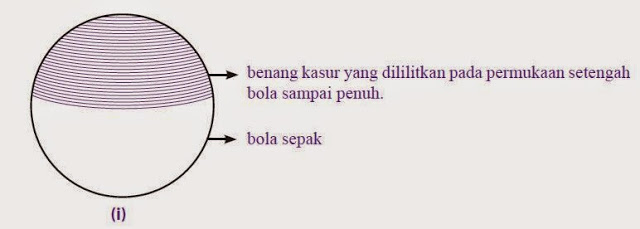
\includegraphics[width=1\textwidth]{figures/bola2.jpg}}
    \caption{gambar bola}
    \label{bola2}
    \end{figure}
4. Buatlah persegi panjang dari kertas karton dengan ukuran panjang sama dengan keliling bola dan lebar sama dengan diameter bola seperti gambar \ref{bola3}.
\begin{figure}[ht]
    \centerline{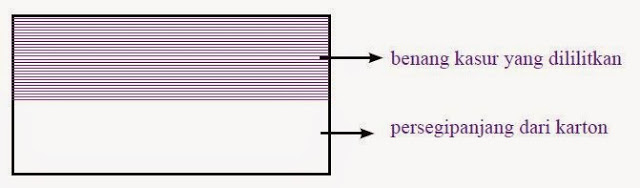
\includegraphics[width=1\textwidth]{figures/bola3.jpg}}
    \caption{beberapa kumpulan gambar yang termasuk dalam bangun ruang}
    \label{bola3}
    \end{figure}
5. Lilitkan benang yang telah digunakan untuk melilit permukaan setengah bola pada persegipanjang yang kamu buat tadi. Lilitkan sampai habis.
6. Jika kamu melakukannya dengan baik, tampak benang tersebut menutupi persegi panjang selebar jari-jari bola (r).
7. Hitunglah luas dari persegi panjang yang telah ditutupi benang tersebut. 
\begin{equation}
Luas permukaan setengah bola = luas persegi panjang
                                           = p × l
                                           = 2πr× r
                                           = 2π r2
\end{equation}

Jadi, luas permukaan bola dirumuskan sebagai berikut :
\begin{equation}
Luas permukaan bola ( L = 4πr2 )
\end{equation}
Keterangan :
L = luas permukaan bola.
r = jari-jari bola.
π = 22/7 atau 3,14

\subsubsection{Asal-usul rumus volume bola}
Cara - cara untuk mengetahui rumus volume bola, dapat dilakukan dengan cara - cara seperti berikut ini : 
1. Siapkan sebuah tempat yang berbentuk setengah bola berjari-jari r (\ref{wadah1}) dan sebuah wadah yang berbentuk kerucut berjari-jari r dan tingginya 2r (\ref{wadah2}).
2. Isikan pasir ke \ref{wadah2} sampai penuh.
3. Pindahkan pasir di dalam \ref{wadah2} ke \ref{wadah1}. Apakah yang terjadi?
\begin{figure}[ht]
    \centerline{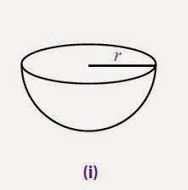
\includegraphics[width=1\textwidth]{figures/wadah1.jpg}}
    \caption{wadah dalam bola}
    \label{wadah1}
    \end{figure}
\begin{figure}[ht]
    \centerline{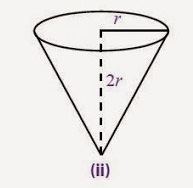
\includegraphics[width=1\textwidth]{figures/wadah2.jpg}}
    \caption{pasir dalam wadah}
    \label{wadah2}
    \end{figure}

Dari cara seperti diatas tersebut, dapat dilihat bahwasanya volume dari pasir yang dituangkan ke dalam wadah setengah bola tidak dapat berubah. Ini berarti, untuk membangun setengah bola, dan kerucut yang berjari-jari sama, dan tinggi kerucut sama dengan dua kali jari-jarinya maka:
\begin{equation}
Volume setengah bola = volume kerucut
1/2 volume bola = 1/3 πr2t
volume bola = 2/3πr2(2r)
                         = 4/3πr3
\end{equation}
Jadi, volume bola tersebut dirumuskan sebagai berikut :
\begin{equation}
Volume bola ( V = 4/3πr3 )
\end{equation}
Keterangan :
V = volume bola.
r = jari-jari bola.
π =22/7 atau 3,14.

Contoh soal :
bola memiliki jari-jari 9 cm, hitunglah volume bola tersebut ?

Jawab :
Diketahui : r = 9 cm
Ditanyakan : volume bola ?
Penyelesaian :
\begin{equation}
V   = 4/3pr3
    = 4/3/ 3 , 14 . (9)3
    = 3.052,08
\end{equation}
Jadi, volume bola tersebut 3.052,08 cm3

\chapter[Diagram Kartesius]
{Pengantar\\ Kartesius}
% Kelompok Diagram Kartesius
% Rahmi Nurdin (1154109)
% Mustari Muammar (1154108)
% Fadillah Firdaus (1154103)

\section{Pengertian Diagram Kartesius}
Diagram Kartesius adalah sistem kooordinat yang terdiri dari dua sumbu yang berisi titik-titik sebagai simbol relasi.
Domain sebagai sumbu horizontal dan kodomain sebagai sumbu vertikal.
Pada koordinat kartesius daerah asal (domain) diletakkan pada sumbu X (sumbu mendatar) dan daerah kawan (kodomain) diletakkan pada sumbu Y (sumbu tegak).
Sedangkan daerah hasilnya merupakan titik (noktah) koordinat pada diagram kartesius. Dari relasi di atas, dapat ditunjukkan diagram kartesiusnya seperti di bawah :
\begin{figure}[ht]
	\centerline{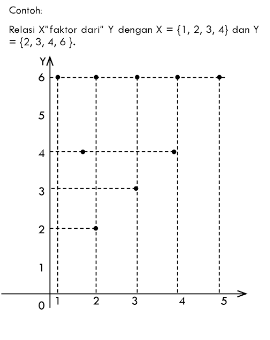
\includegraphics[width=1\textwidth]{figures/rahmi1.PNG}}
	\caption{hubungan antar titik pada diagram kartesius.}
	\label{rahmi1}
	\end{figure}

Diagram Kartesius merupakan suatu bangunan atas empat bagian yang batasi oleh dua buah garis yang berpotongan tegak lurus pada titik-titik (  X, Y ). 
Dimana X merupakan rata-rata dari rata-rata skor tingkat pelaksanaan atau kepuasan konsumen dari sebuah faktor atribut 
dan Y adalah rata-rata skor tingkat kepentingan seluruh faktor atau atribut yang mempengaruhi kepuasan konsumen.
Seluruhnya ada K faktor. Rumus berikutnya yang digunakan adalah :
\begin{figure}[ht]
	\centerline{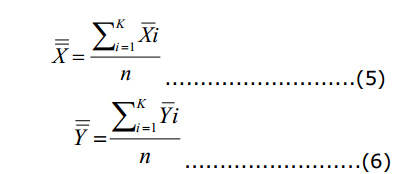
\includegraphics[width=1\textwidth]{figures/rahmi2.PNG}}
	\caption{rumus mencari K faktor.}
	\label{rahmi2}
	\end{figure}

Dimana :K = Banyaknya faktor atau atribut yang mempengaruhi kepuasan konsumen 
Diagram Kartesius	
\begin{figure}[ht]
	\centerline{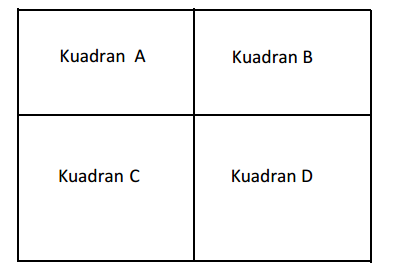
\includegraphics[width=1\textwidth]{figures/rahmi3.PNG}}
	\caption{penentuan kuadran pada diagram kartesius.}
	\label{rahmi3}
	\end{figure}

Gambar 1. Diagram Kartesius



Kuadran A
Pada posisi ini, jika dilihat dari kepentingan konsumen, atribut-atibut produk berada pada tingkat tinggi, tetapi jika di lihat dari kepuasannya, 
konsumen merasakan tingkat yang rendah, sehingga konsumen menuntut adanya perbaikan atribut tersebut.
Kuadran B
Pada posisi ini, jika dilihat dari kepentingan konsumen, atribut-atribut produk berada pada tingkat tinggi, dan dilihat dari kepuasannya, 
konsumen merasakan tingkat yang tinggi juga.
Kuadran C
Pada posisi ini, jika dilihat dari kepentingan konsumen, atribut-atribut produk kurang dianggap penting, tetapi jika dilihat dari tingkat kepuasan konsumen cukup baik.
Namun, konsumen mengabaikan atributatribut yang terletak pada posisi ini.
Kuadran D
Pada posisi ini, jika dilihat dari kepentingan konsumen, atribut-atribut produk kurang dianggap penting, tetapi jika dilihat dari tingkat kepuasanya, konsumen merasa
sangat puas.


\section{Penghitungan Rumus Diagram Kartesius}
\subsection{meghitung rumus, mencari titik}

Kartesius digunakan untuk menentukan tiap titik dalam bidang dengan menggunakan dua bilangan yang biasa disebut koordinat x dan koordinat y.
\begin{figure}[ht]
	\centerline{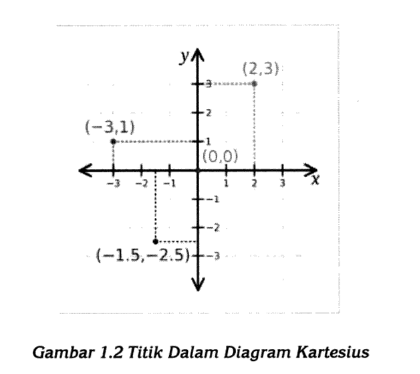
\includegraphics[width=1\textwidth]{figures/rahmi9.PNG}}
	\caption{penentuan titik pada kuadran katesius.}
	\label{rahmi9}
	\end{figure}

Sebuah titik dalam Diagram Kartesius, mengandung dua buah informasi yakni sumbu (x,y), seperti tampak pada Gambar 1.2. 
Yaitu titik (2,3) adalah titik dimana nilai x=2 dan y=3. Daerah ini dikenal dengan kuadran I, dimana nilai x dan y adalah positif.
\begin{figure}[ht]
	\centerline{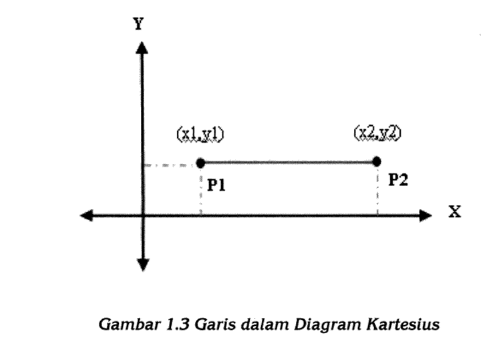
\includegraphics[width=1\textwidth]{figures/rahmi10.PNG}}
	\caption{penentuan garis pada kuadran katesius.}
	\label{rahmi10}
	\end{figure}

Dari dua buah titik diagram kartesius, bisa ditarik menjadi sebuah garis. Artinya pada sebuah garis memiliki titik awal


\section{Contoh Penerapan/Pemetaan Diagram Kartesius}
Tujuan digunakannya diagram kartesius adalah untuk melihat secara lebih terperinci mengenai atribut-atribut yang perlu untuk dilakukan perbaikan. 
Langkahlangkah sebelum memetakan data ke diagram kartesius ini, adalah terlebih dahulu dengan menentukan nilai rata-ratasetiap atribut yaitu X dan Y, 
dimana nilai perhitungannya telah kita peroleh dari perhitung yang dilakukan sebelumnya.
Adapun hasil pembagian setiap atribut pada setiap kuadaran ditampilkan pada gambar 2
\begin{figure}[ht]
	\centerline{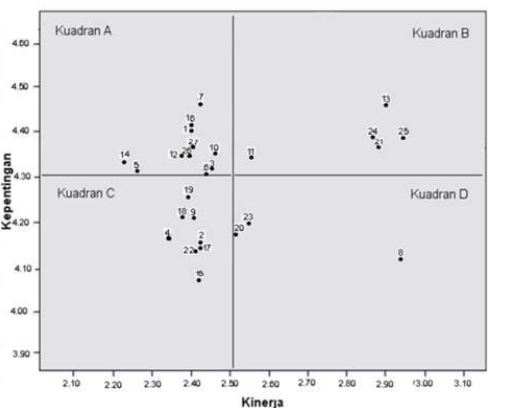
\includegraphics[width=1\textwidth]{figures/rahmi4.PNG}}
	\caption{.}
	\label{rahmi4}
	\end{figure}


Gambar 2. Diagram Kartesius
Setelah dilakukan perhitungan menggunakan diagram kartesius didapat hasil atribut-atribut yang harus diperbaiki adalah atribut yang berada pada kuadran A.
Adapun atribut yang harus diperbaiki pada kuadran A adalah :
Tabel 2 Hasil Perhitungan Diagram Kartesius pada Kuadran A	
\begin{figure}[ht]
	\centerline{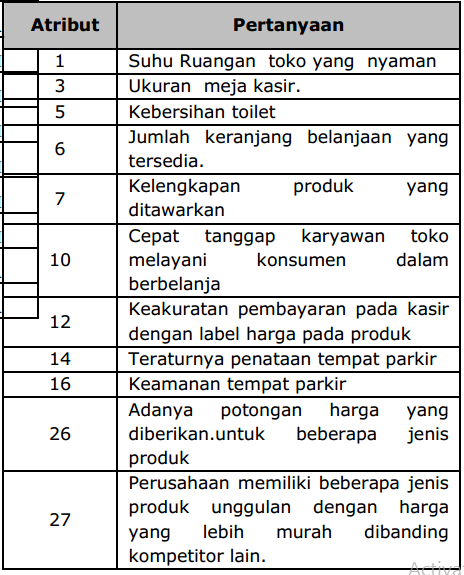
\includegraphics[width=1\textwidth]{figures/rahmi5.PNG}}
	\caption{.}
	\label{rahmi5}
	\end{figure}


Untuk atribut-atribut yang harus dipertahanan oleh pihak perusahaan setelah dilakukannya perhitungan menggunakan diagram kartesius adalah atribut-atribut
yang berada pada kuadran B, karena pada atribut yang berada pada kuadran B dianggap pelanggan sudah dapat memenuhi apa yang mereka inginkan. 
Adapun atribut yang harus dipertahankan dapat dilihat pada
Tabel 3.
Tabel 3. Hasil Perhitungan Diagram Kartesius
pada Kuadran B
\begin{figure}[ht]
	\centerline{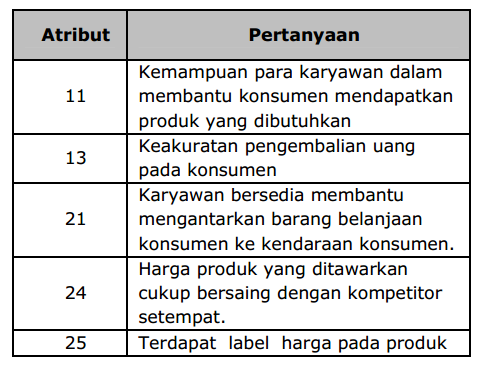
\includegraphics[width=1\textwidth]{figures/rahmi6.PNG}}
	\caption{.}
	\label{rahmi6}
	\end{figure}

Atribut yang memiliki penilaian yang rendah karena atribut-atribut ini kurang dianggap penting oleh pelanggan dan perusahaan juga tidak memberikan pelayanan atau perhatian khusus, 
atribut ini dianggap tidak memberikan dampak yang besar bagi perusahaan.
Adapun atribut-atribut yang berada pada kuadran C dapat dilihat pada Tabel 4.
Tabel 4. Hasil Perhitungan Diagram Kartesius pada kuadran C
\begin{figure}[ht]
	\centerline{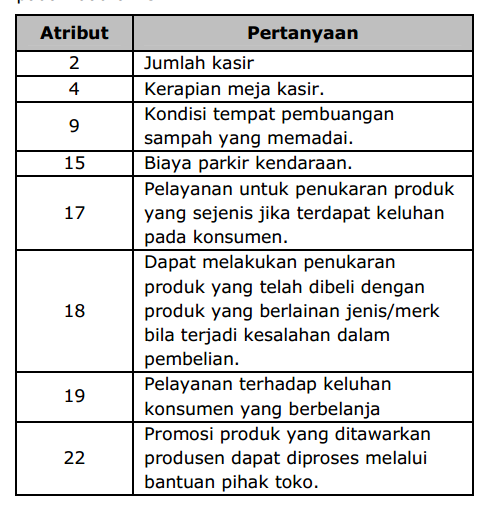
\includegraphics[width=1\textwidth]{figures/rahmi7.PNG}}
	\caption{.}
	\label{rahmi7}
	\end{figure}

Untuk atribut yang ada pada kuadran D adalah atribut yang tidak dianggap penting bagi pelanggan, namun pihak perusahaan memberikan pelayanan yang berlebihan 
sehingga atribut ini dianggap berlebihan.
Adapun atribut yang berada pada kuadran D dapat dilihat pada Tabel 5.
Tabel 5. Hasil Perhitungan Diagram Kartesius
pada Kuadran D	
\begin{figure}[ht]
	\centerline{\includegraphics[width=1\textwidth]{figures/rahmi8.PNG}}
	\caption{.}
	\label{rahmi8}
	\end{figure}


Diagram Kartesius
Dari hasil perhitungan yang telah dilakukan sebelumnya, terdapat 17 atribut yang perlu dilakukan perbaikan (Action) danterdapat 10 atribut yang perlu mendapat
perhatian untuk dipertahankan oleh pihak perusahaan (Hold). Diagram Kartesius Dari hasil pemetaan yang dilakukan pada diagram kartesius dapat terlihat beberapa
atribut yang perlu untuk dilakukannya perbaikan dan atribut-atribut perlu untuk dipertahankan oleh pihak perusahaan yang terbagi kedalam kuadran-kuadran (A, B, C
dan D) sesuai dengan tingkat kesesuaian antara tingkat kepentingan pelanggan dan kinerja perusahaan, yaitu dengan tingkat kesesuaian sebesar 58.374.
Adapun hasil pemetaannya adalah sebagai berikut:
Kuadran A
Kuadran A adalah wilayah yang berisikan atribut-atribut yang dianggap penting oleh pelanggan, namun dalam kenyataannya atribut-atribut ini masih belum sesuai
dengan yang diharapkan oleh pelanggan. Dalam hal ini perusahaan perlu melakukan perbaikan sebaik mungkin untuk meningkatkan kepuasan pelanggan terhadap
atribut yang termasuk kedalam kuadran A. Dari diagram kartesius yang dibuat, diketahui bahwa atribut yang termasuk dalam kuadran A yaitu atribut 1, 3, 5, 6, 7,
10, 12, 14, 16, 26, 27.
Adapun beberapa hal yang sebaiknya perlu dilakukan guna perbaikan atau penyesuaian terhadap beberapa hal yang menjadi  prioritas diatas yang pertama antara lain
perlunya dilakukan penambahan alat pendingin ruangan untuk dapat menjaga suhu ruangan demi kenyamanan pelanggan,Penambahan ukuran meja kasir agarbarang-barang belanjaan yang telah dipilih
tidak merepotkan pelanggan ataupun kasir. Selain itu juga perlu dilakukannya perbaikan ataupun pembersihan ruangan toilet dan pendukung lainnya seperti ketersediaan air
sehingga pelanggan yang menggunakan akan merasa lebih nyaman, penambahan jumlah keranjang belanjaan yang disediakan perusahaan, Lebih melengkapi jenis-jenis
produk yang ditawarkan dengan mempertimbangkan tempat penyimpanan serta waktu-waktu tertentu seperti hari-hari besar nasional dan lain sebagainya,Memberikan pengarahan kepada para
karyawan mengenai pentingnya berinisiatif dalam melayani pelanggan yang membutuhkan bantuan tanpa harus dimintaitolong terlebih dahulu oleh pelanggan.
Dapat juga dilakukan penambahan papan informasi berupa lokasi produk yang tersedia untuk dapat mengurangi frekuensi terjadi atau timbulnya pertanyaan dari para
pelanggan mengenai produk yang akan mereka beli, perbaikan ataupun penyesuaian secara berkala antara labellabel harga yang tertera pada produk yang ditawarkan dengan perubahan-perubahan
harga yang terjadi, penataan tempat parkir yang dapat dilakukan dengan memberikan garis-garis pembatas kendaraan, ataupun dengan menambahkan tukang parkir untuk
dapat menanggulangi keamanan dan penataan tempat parkir kendaraan, penyusunan program-program promo secara berkala, seperti pemberian diskon denganjumlah pembelian tertentu ataupun dengan
memberikan voucer belanja dengan nilai tertentu untuk dapat lebih menarik pelanggan, dan sebaiknya perusahaan memiliki atau beberapa jenis produk tertentu
yang diunggulkan dengan harga yang lebih murah dibandingkan dengan kompetitor lainnya sebagai penarik.
Kuadran B
Kuadran B adalah daerah yang memuat atribut-atribut yang dianggap penting oleh pelanggan, dan atribut-atribut tersebut dianggap telah sesuai dengan keinginan
pelanggan sehingga tingkat kepuasan pelanggan relatif lebih tinggi, sehingga perlu untuk dipertahankan oleh pihak perusahaankarena sudah bisa memberikan pelayanan
sesuai dengan keinginan pelanggan sehingga konsumen merasa puas. Adapun atribut yang termasuk kedalam kuadran ini adalah:11, 13, 21, 24, 25.
Kuadran C
Kuadran C adalah Daerah yang berisikan atribut-atribut yang dianggap kurang penting oleh pelanggan dan pada kenyataannya kinerja pihak perusahaanpundinilai kurang memuaskan. Tetapi tidak
menutup kemungkinan Kuadran C pada waktu yang akan datang menjadi perhatian yang penting oleh pelanggan, sehingga perusahaan juga harus mempertimbangkan
hal tersebut. Adapun atribut yang termasuk kedalam kuadran ini adalah: 2, 4, 9, 15, 17, 18, 19, 22.
Kuadran D
Kuadran D adalah wilayah yang memuat atribut-atribut yang dianggap kurang penting oleh pelanggan dan kinerja yang dilakukan oleh pihak perusahaan dirasakan
terlalu tinggi atau berlebihan, sehingga perusahaan tidak perlu melakukan perbaikan. Adapun atribut yang termasuk kedalam kuadran ini adalah: 8, 20, 23.

\section{Pengertian Bidang atau Diagram Cartesius}

Dalam mempelajari materi himpunan, fungsi, dan persamaan garis lurus kita akan mengenal yang namanya bidang atau diagram Cartesius. Apa itu bidang atau diagram Cartesius?

Diagram Cartesius adalah sistem kordinat yang digunakan untuk meletakan titik pada penggambaran objek berdasarkan pemasukan nilai pada sumbu x dan nilai pada sumbu y dimana titik pertemuan ini nilai dari sumbu x dan sumbu y titik kordinat dibentuk. Jadi, diagram Cartesius digunakan untuk menentukan tiap titik dalam bidang dengan menggunakan dua bilangan yang biasa disebut koordinat x dan koordinat y dari titik tersebut. Di mana x disebut absis dan y disebut ordinat.

Titik-titik pada koordinat Cartesius merupakan pasangan titik pada sumbu-x dan sumbu-y (x, y). Perpotongan antara sumbu-x dan sumbu-y di titik 0 (nol) disebut pusat koordinat. Untuk bagian atas sumbu y bernilai positif, sedangkan pada bagian bawah sumbu y bernilai negatif. Begitu juga pada sebelah kanan sumbu x bernilai positif, sedangkan pada sebelah kiri sumbu x bernilai negatif. Untuk contohnya silahkan lihat gambar di bawah ini. 
\begin{figure}[ht]
	\centerline{\includegraphics[width=1\textwidth]{figures/cau100.PNG}}
	\caption{penentuan garis/titik dalam diagram kartesius}
	\label{cau100}
	\end{figure}

Perhatikan diagram Cartesius pada gambar di atas. Warna ungu (violet) merupakan pusat koordinat yaitu titik (0,0) yang artinya sumbu x dan y bernilai nol. Untuk warna hijau, pada sumbu x bernilai 2 dan sumbu y bernilai 3 maka koordinat dalam bidang cartesius ditulis (2,3). Untuk warna merah, pada sumbu x bernilai  – 3 dan sumbu y bernilai 1 maka koordinat dalam bidang cartesius ditulis (– 3, 1). Sedangkan untuk warna biru, pada sumbu x bernilai  – 3 dan sumbu y bernilai 1 maka koordinat dalam bidang cartesius ditulis (–1.5 , –2.5).

Menurut wikipedia, istilah Cartesius digunakan untuk mengenang ahli matematika sekaligus filsuf dari Perancis bernama Descartes. Beliau memiliki peranan yang sangat besar dalam menggabungkan aljabar dan geometri (Cartesius adalah latinisasi untuk Descartes). Hasil kerjanya sangat berpengaruh dalam perkembangan geometri analitik, kalkulus, dan kartografi.




\chapter[Benua]
{Pengantar\\ benua}
% Kelompok Sejarah Benua dan Koordinat
% Agien Farhan S (1154012)
% Berlin Mitra Putra A (1154061)
% Indra Riksa Herlambang (1154051)
% Indra Saryoni Simanjuntak (1154115)
% Kindi Herdiansyah (1154048)

\section{Sejarah Benua}

\subsection{Benua pertama}
Mantel konveksi, proses yang mendorong lempeng tektonik adalah hasil dari aliran panas dari dalam bumi ke permukaan bumi \cite{suryasejarah}.Termasuk juga penciptaan lempeng tektonik di pegunungan bawah laut. Lempeng ini dihancurkan oleh subduksi di zona subduksi. Pada awal eon Arkean \ref{PetaAmerikaUtara} (sekitar 3 miliar tahun yang lalu) mantel itu jauh lebih panas mungkin sekitar 1600° C, sehingga proses konveksi terjadi lebih cepat.

Kerak bumi mulai terbentuk saat permukaan bumi mulai memadat, menghilangkan bekas-bekas pergeseran lempeng tektonik Hadean. Namun, diperkirakan kerak bumi memiliki komposisi Basalt seperti Kerak samudera .Potongan kerak benua besar yang pertama, muncul saat akhir masa Hadean, sekitar 4 miliar tahun yang lalu.  Kraton adalah bagian kecil yang tersisa dari benua pertama. Potongan-potongan yang terjadi pada akhir Hadean sampai awal Arkean membentuk inti lempengan yang tumbuh menjadi benua seperti sekarang.

Batuan tertua ditemukan di Laurentia, Kanada, yang berupa tonalit yang berumur sekitar 4 miliar tahun. Bebatuan ini menunjukkan jejak metamorfosis oleh suhu tinggi,  dan biji-bijian sedimen yang terkena erosi selama terbawa oleh air, yang menunjukkan terdapat sungai dan laut pada 4 miliar tahun yang lalu.

\begin{figure}[ht]
    \centerline{\includegraphics[width=1\textwidth]{figures/PetaAmerikaUtara.JPG}}
    \caption{Peta geologi Amerika Utara, kode warna menunjukan usia. Warna merah dan pink menunjukkan batuan dari masa eon Arkean.}
    \label{PetaAmerikaUtara}
    \end{figure}


\subsection{Benua raksasa pada masa Proterozoikum} 
Rekonstruksi pergerakan lempeng tektonik pada 250 juta tahun terakhir ( pada era Kenozoikum dan mesozoikum) dapat dilakukan dengan melihat kecocokan benua, anomali magnetik dasar laut, dan kutub paleomagnetik \cite{suryasejarah}. Para ahli tidak menemukan kerak samudera yang terbentuk sebelum waktu tersebut, sehingga rekonstruksi sebelum waktu tersebut sulit untuk dilakukan. Kutub paleomagnetik dilengkapi dengan bukti geologi seperti sabuk orogenik, yang menandai tepi lempeng kuno, dan distribusi flora dan fauna pada masa itu.

Sepanjang sejarah bumi, ada saat dimana benua bertabrakan dan membentuk benua raksasa, yang kemudian pecah menjadi benua baru. Sekitar 1000–830 juta tahun yang lalu, benua yang paling luas bersatu membentuk sebuah benua raksasa Rodinia. Sebelum Rodinia terbentuk, diperkirakan telah terbentuk terlebih dahulu Columbia atau Nuna pada awal sampai pertengahan masa Proterozoikum.

Setelah Rodinia pecah sekitar 800 juta tahun lalu, benua-benua tersebut kemungkinan telah membentuk benua raksasa lain yang berumur pendek yaitu , Pannotia \ref{BenuaRaksasaPannotia} pada 550 juta tahun lalu. Hipotetis benua raksasa mengacu pada Pannotia atau Vendia. Bukti yang memperkuat hipotesis tersebut adalah fase tabrakan benua yang diketahui sebagai orogeni Pan-Afrika, yang bergabung dengan benua Afrika , Amerika Selatan, Antartika dan Australia. Keberadaan Pannotia ditentukan oleh terjadinya retakan antara Gondwana (sebagian besar termasuk daratan di belahan bumi selatan, serta meliputi Semenanjung Arab dan anak benua India) dan Laurentia (kira-kira setara dengan Amerika Utara pada masa sekarang).Hal ini meyakinkan bahwa pada akhir masa eon Proterozoikum, sebagian besar benua bergabung dalam posisi di sekitar kutub selatan.

\begin{figure}[ht]
    \centerline{\includegraphics[width=1\textwidth]{figures/BenuaRaksasaPannotia.JPG}}
    \caption{Rekonstruksi benua raksasa Pannotia (warna kuning) pada 550 juta tahun lalu.}
    \label{BenuaRaksasaPannotia}
    \end{figure}


\subsection{Bukti Tersusunnya Benua Kuno}
Terdapat bukti dari para ahli yang digunakan untuk memperkirakan tersusunnya benua kuno.
Menurut Alfred Wegener(1880-1930), bahwa semua benua pernah bersatu kemudian berpecah menjadi sekarang ini dan benua yang bersatu itu dinamakan Pagaea (Benua Besar)\cite{hallam1975alfred}. Kemudian para ahli meneliti tentang benua dan membuat spekulasi-spekulasi teoritis yaitu melihat pada peta bahwa benua saling melengkapi dilihat dari garis pantai yang saling melengkapi seperti bagian puzzle. Kemudian meneliti fosil, bukti lain dari kehidupan lampau yaitu Mesosaurus. Mesosaurus adalah reptilia purba yang hanya hidup di air tawar dan ternyata hanya ada dua kawasan didunia yang memiliki fosil Mesosaurus ini yaitu Pantai Timur Amerika Selatan dan Pantai Barat Afrika. Kesimpulannya, fosil yang sama telah ditemukan di dalam batuan di kedua sisi lautan. Kemudian bukti korelasi batuan dan pegunungan telah ditemui di kedua belah sisi lautan. Yaitu meneliti banjaran pegunungan di Timur Laut Amerika Serikat dan banjaran pegunungan di Utara Eropa. Keduanya sangat sepadan atau keduanya tersusun daripada jenis batuan yang sama. Kemudian bukti data iklim masa lalu, terbukti pada Glacial Striations atau terdapat bentuk goresan pada batuan dan ini dapat dilihat dari hutan hujan tropika Amerika Selatan dan Afrika saat ini terdapat goresan glasier. Kesimpulannya adalah arang batu telah ditemukan di kawasan sejuk dan bukti glasier telah ditemui di kawasan panas berarti sebelumnya ada kemungkinan benua bersatu.

\section{Sejarah Koordinat}
Menurut ahli sejarah yang bernama Heroditus (450 M) menyatakan bahwa geometri berasal dari Mesir. Rane Discartes seorang matematikawan, yang lahir di sebuah Desa La Haye Prancis pada tahun 1596, adalah orang yang memiliki ketertarikan di bidang geometri. Rane Descrates telah menemukan sebuah metode untuk menyajikan sebuah titik sebagai bilangan berpasangan pada sebuah bidang datar. Bilangan-bilangan tersebut terletak pada dua garis yang saling tegak lurus antara satu dengan lainnya dan berpotongan di sebuah titik (0,0) dinamakan Origin , dan biasanya disimbolkan dengan huruf kapital O (0,0).
Bidang tersebut dinamakan bidang KOORDINAT atau yang lebih dikenal dengan bidang KARTESIUS.

\section{Sistem Koordinat}
Sistem koordinat dimaksudkan untuk memberikan peng-alamat-an terhadap setiap lokasi di permukaan bumi. Peng-alamatan dengan sistem kordinat didasarkan atas jarak timur-barat dan utara-selatan suatu tempat dari suatu titik pangkal tertentu. Jarak diukur dalam satuan derajat sudut yang dibentuk dari dari titik pangkal ke posisi tersebut melalui pusat bumi. Sedangkan titik pangkal ditetapkan berada di
perpotongan belahan utara-selatan bumi (garis katulistiwa) dengan garis yang membelah bumi timur- barat\cite{zuhdi2012sistem}.

Koordinat diambil untuk menjadi bilangan riil dalam matematika dasar, tetapi mungkin bilangan kompleks atau elemen-elemen dari sistem yang lebih abstrak. Penggunaan sistem koordinat memungkinkan masalah dalam angka untuk diterjemahkan ke dalam masalah-masalah tentang geometri dan juga sebaliknya.

\subsection{Sistem Koordinat Dua Dimensi}
\subsubsection{Sistem Koordinat Kartesius}
Koordinat Cartesius bukan merupakan satu-satunya jalan untuk menunjukkan kedudukan suatu titik pada bidang. Karena bentuk geometris di alam tidak selalu berupa kotak-kotak atau persegi panjang, namun adakalanya berbentuk lingkaran\cite{mufidah2015solusi}.Sistem koordinat Kartesius pada dua dimensi umumnya didefinisikan dengan dua buah sumbu yang saling tegak lurus antara satu dengan yang lainnya, yang keduanya terletak pada satu bidang (bidang xy). Sumbu horizontal(x), dan sumbu vertikal(y). Lalu, pada sistem koordinat tiga dimensi, ditambahkan sumbu yang lain yang sering diberi label z. Sumbu-sumbu tersebut ortogonal antar satu dengan yang lainnya. Titik pertemuan antara kedua sumbu, titik asal, pada umumnya diberi label 0. Setiap sumbu juga memiliki besaran panjang unit, dan setiap panjang tersebut diberi tanda dan membentuk semacam grid. Untuk mendeskripsikan suatu titik tertentu pada sistem koordinat dua dimensi, nilai absis(x), lalu diikuti dengan nilai ordinat(y). Dengan demikian, format yang dipakai selalu (x dan y) dan urutannya tidak dibalik-balik.

Gambar \ref{koordinat} Tanda panah yang ada pada sumbu berarti panjang sumbunya tak terhingga pada arah panah tersebut.

\begin{figure}[ht]
    \centerline{\includegraphics[width=1\textwidth]{figures/koordinat.JPG}}
    \caption{Keempat kuadran sistem koordinat Kartesius}
    \label{koordinat}
    \end{figure}

Pilihan huruf-huruf didasari oleh konvensi, yaitu huruf-huruf yang dekat akhir(x dan y) yang digunakan untuk menandakan variabel dengan nilai yang tidak diketahui, sedangkan huruf-huruf yang lebih dekat awal digunakan untuk menandakan nilai yang diketahui. Karena kedua sumbu saling bertegak lurus satu sama lain, bidang xy terbagi menjadi empat bagian yang disebut dengan kuadran, yang pada Gambar 3 ditandai dengan angka I, II, III, dan IV. Menurut konvensi yang berlaku, keempat kuadran tersebut diurutkan mulai dari yang kanan atas (kuadran I), melingkar melawan arah jarum jam (lihat Gambar 3). Pada kuadran I, kedua koordinat (x,y) bernilai positif. Pada kuadran II, koordinat x bernilai negatif dan koordinat y bernilai positif. Pada kuadran III, kedua koordinat mempunyai nilai negatif, dan pada kuadran IV, koordinat x bernilai positif dan y bernilai negatif. (lihat gambar \ref{contoh} dibawah ini).

\begin{figure}[ht]
    \centerline{\includegraphics[width=1\textwidth]{figures/contoh.JPG}}
    \caption{Nilai x dan y pada Kuadran I,II,III,IV}
    \label{contoh}
    \end{figure}

\subsubsection{Sistem Koordinat Polar}
Pada sistem koordinat polar, sepasang koordinat polar suatu titik ditulis dengan (𝑟,𝜃)\cite{mufidah2015solusi}.Konsep dari sudut dan radius sudah diterapkan oleh orang-orang pada zaman dahulu se-abad sebelum masehi. Para astronom yunani dan astrologhipparcuhus (190-120 BCE) menemukan sebuah tabel dari fungsi dawai yang memberikan panjang dawai dari setiap sudut dan terdapat referensi dari penggunaan koordinat polar untuk mengetahui posisi bintang.

Sejak abad ke-8 yang lalu, astronom mengembangkan cara untuk mengira-ngira dan menghitung arah dari mekah, kaabah- beserta jaraknya-dari seluruh lokasi dari bumi. Penghitungan penting yaitu penggantian dari koordinat polar ekuatorial dari mekkah kedalam bentuk koordinat polar hampir sama pada sistem yang merupakan pusat dari lingkaran besar melewati daerah yang dilewati dan kutub bumi, serta sudut polar yaitu garis yang melewati daerah tersebut dan titik antipodal.

Dalam Method of fluxion (tertulis 16711) Sir Isaac Newton menentukan hubungan antara koordinat polar, yang kemudian ia sebut dengan “ tujuh cara untuk spiral, dan sembilan sistem koordinat. 

\section{Geometri Koordinat}
 Pembelajaran subtajuk-subtajuk Geometri Koordinat, iaitu jarak antara dua titik, pembahagian tembereng garis, luas poligon, persamaan garis lurus, garis lurus selari dan garis lurus serenjang, persamaan lokus yang melibatkan jarak antara dua titik dan menentukan hubungan antara pencapaian responden dalam topik pelajaran\cite{shong2013analisis}.
 
 \subsection{Sketsa Grafik Garis}
 Sketsa grafik garis merupakan salah satu materi yang membahas mengenai penggambaran grafik garis lurus pada bidang kartesius berdasarkan persamaan yang diberikan. Materi ini mirip dengan metode penggambaran garis yang ada atau diajarkan pada aljabar. Maka jika sudah menguasai materi aljabar, sketsa grafik garis bukan masalah untuk dipelajari. Dalam menggambar grafik garis lurus, pertama harus melakukan pencarian pada nilai x dan y pada bidang kartesius dari persamaan yang sudah ada. Setelah nilai x dan y pada bidang kartesius telah di-temukan tentu bisa menentukan titiknya dan langsung menggambar garis tersebut.
 
 \subsection{Persamaan Garis Lurus}
 Persamaan garis lurus dapat di-definisikan sebagai perbandingan selisih nilai x dan y yang sudah melangkahi 2 titik pada garis. 
 Persamaan garis lurus terdapat satu komponen Gradien yaitu kecenderungan sebuah garis, gradien biasa dilambangkan dengan huruf m.
 Dalam materi persamaan garis lurus terdapat materi pokok seperti menentukan \"gradien" garis lurus, \"kedudukan" garis lurus,
 \"persamaan" garis melalui satu titik merupakan gradien, dan \"persamaan" garis melalui dua titik.
 
 \subsection{Pesamaan Lingkaran}
 Persamaan lingkaran adalah persamaan titik koordinat yang membentuk sebuah lingkaran pada bidang kartesius. Pada konsep ini jari lingkaran yang telah terbentuk adalah jarak dari himpunan titik koordinat ke titik pusat atau sebaliknya.Pada persamaan lingkaran yang dapat dipelajari seperti lingkaran yang memiliki pusat (0,0), lingkaran yang memiliki pusat (a,b).
 
 \subsection{Program Linear}
 Program linear adalah metode matematika yang digunakan untuk menyelesaikan soal-soal yang memiliki batas persamaan linear. Secara umum program linear terbagi atas 2 bagian yaitu fungsi kendala dan fungsi objektif. Penyelesaian program linear model matematika adalah suatu metode penerjemahan permasalahan ke dalam bentuk matematika, sehingga soal tersebut bisa diselesaikan secara matematis.
 
 \subsection{Pembelajaran Geometri Koordinat}
 Geometri Koordinat merupakan materi yang memberika pengujian ketrampilan dalam geometri dan aljabar.
 Jika sudah menguasai materi geometri dan aljabar maka bisa dinyatakan geometri koordinat tidak lagi membuat sulit untuk dipelajari.


%\chapter[Sejarah Bumi]
%{Pengantar\\ Sejarah Bumi}
%% Nama Kelompok : Kelompok 4
% Akbar Pambudi Utomo (1154094) 
% Andi Nurfadilah Ali (1154041)
% Andi Wadi Afryandika (1154113)
% Hanna Theresia Siregar (1154009)
% Julham Ramadhana (1154069)
% Pebridayanti Hasibuan (1154118)

\section{Sejarah Bumi}
Bumi merupakan planet atau rumah kita dalam kedudukan di tata surya. peradaban kuno percaya bahwa bumi itu datar, dengan langit berputar-putar sekali sehari. secara umum yang diyakini bahwa kehidupan di Bumi dimulai di Bumi itu sendiri, beberapa waktu setelah terbentuknya planet antara 4000-5000 juta tahun yang lalu. namun ada yang berpendapat bahwa kehidupan diluar bumi itu ada, tetap kita tidak memiliki bukti pasti tentang kehidupan di tempat lain. yang perlu kita ketahui bumi berada pada galaksi bimasakti dimana terdapat matahari sebagai sistem bintang.
Dalam Geologi sendiri atau biasa disebut sebagai ilmu pengetahuan tentang Kebumian yang mempelajari segala sesuatu mengenai planet Bumi beserta isinya yang pernah ada. Dalam Geologi juga akan dibahas tentang sifat-sifat dan bahan- bahan yang membentuk bumi itu apa, serta struktur dan proses-proses yang bekerja baik didalam maupun dibagian teratas permukaan bumi, kedudukannya di Alam Semesta hingga sekarang. Geologi merupakan ilmu pengetahuan yang komplek, mempunyai pembahasan materi yang beraneka ragam namun juga merupakan ilmu pengetahuan yang enak dipelajari. Sebagai landasan prinsip untuk dapat mempelajari ilmu geologi adalah bahwasanya kita harus menganggap bumi ini sebagai suatu benda yang secara dinamis berubah sepanjang masa, setiap saat dan setiap detik. 
Pemikiran geologi modern dikenalkan oleh Huttonian revolution mengemukakan pemikiran-pemikirannya sebagai berikut:
1. Bahwasanya proeses-proses alam yang sekarang ini menyebabkan perubahan pada permukaan bumi, juga bekerja sepanjang umur dari bumi ini. 
2. Ia juga mengamati bahwa proses-proses tersebut yang walaupun bekerja sangat lambat, tetapi pada akhirnya mampu menyebabkan terjadinya perubahan-perubahan yang sangat besar pada bumi. 
3. Bahwa bumi ini sangat dinamis, yang berarti mengalami perubahan-perubahan yang terus-menerus mengikuti suatu pola daur (siklus) yang berulang-ulang.
Bumi sendiri berada di kawasan dimana terjadinya tumpang tindih antara litosfer (daratan) bagian padat dari bumi, hidrosfer (perairan), dan atmosfer (udara) yang menyelubungi bumi dengan zarah-zarah dan benda-benda yang mengisinya.
Dalam sejarah terbentuknya bumi sewaktu SMA kita pernah mempelajari teori-teori terbentuknya bumi dalam pelajaran geografi.\cite{wetherill1990formation}

\subsection{Teori-teori terbentuknya Bumi}
\subsubsection{1.Teori Kabut Kant-Laplace}
\begin{figure} [ht]
	\centerline{\includegraphics[width=1\textwidth]{figures/teorikabutnebula.JPG}}
	\caption{Gambar Teori Nebula}
	\label{teorikabutnebula}
	\end{figure}
	Pada Gambar berikut \ref{teorikabutnebula} adalah gambar dari Teori Kabut Nebula.
Teori ini dikenal dengan teori kabut (nebula) yang dikemukakan oleh Immanuel Kant (1755) dan Pierre de Laplace (1796). dalam teori ini dikemukakan bahwa di jagat raya terdapat gas yang kemudian berkumpul menjadi kabut(nebula). gaya tarik-menarik antargas ini membentuk kumpulan kabut yang sangat besar dan berputas semakin cepat sehingga materi kabut bagian khatulistiwa terlempar memisah dan memadat(karena pendinginan), bagian yang terlempar inilah yang kemudian menjadi sebuah planet dalam tatasurya. Bumi baru terus bertumbuh sampai suhu interiornya cukup panas untuk melelehkan logam siderofil. Dengan massa jenis yang lebih tinggi dari silikat, akhirnya logam ini tenggelam. Proses ini terjadi 10 juta tahun setelah Bumi mulai terbentuk, dan menghasilkan struktur Bumi yang berlapis-lapis dan mengakibatkan terbentuknya medan magnet. J. A. Jacobs merupakan orang pertama yang menunjukkan bahwa inti dalam—bagian dalam yang padat berbeda dari inti luar yang padat—membeku dan mengembang keluar inti luar yang cair dikarenakan bagian dalam bumi yang makin mendingin (sekitar 100° C per miliar tahun. Ekstrapolasi dari pengamatan ini memperkirakan bahwa inti terbentuk pada masa 2–4 miliar tahun yang lalu. Jika ini benar maka berarti bahwa inti bumi bukanlah fitur primordial yang berasal selama pembentukan planet.

\subsubsection{2.Teori Planetesimal}
\begin{figure} [ht]
	\centerline{\includegraphics[width=1\textwidth]{figures/teoriplanetesimal.JPG}}
	\caption{Gambar Teori Planetesimal}
	\label{teoriplanetesimal}
	\end{figure}
	Pada Gambar berikut \ref{teoriplanetesimal} adalah gambar dari Teori Planetesimal.
seabad kemudian sesudah teori kabut tersebut muncul teori Planetesimal yang dikemukakan oleh Chamberlin dan Moulton. Teori ini mengungkapkan bahwa pada mulanya telah terdapat Matahari asal. pada suatu ketika, matahari asal ini didedakti sebuah bintang besar yang menyebabkan terjadinya penarikan pada bagian matahari. Akibat tenaga tarik menarik tadi, terjadilah ledakan yang dasyat. Gas yang meledak ini keluar dari atmosfer matahari, kemudian mengembun dan membeku sebagai benda-benda yang padat(disebut planetesimal). Planetesimal ini dalam perkembangannya menjadi planet-planet, dan salah satunya planet bumi kita.

\subsubsection{3.Teori Pasang Surut Gas}
\begin{figure} [ht]
	\centerline{\includegraphics[width=1\textwidth]{figures/teoripasangsurut.JPG}}
	\caption{Gambar Pasang Surut}
	\label{teoripasangsurut}
	\end{figure}
	Pada Gambar berikut \ref{teoripasangsurut} adalah gambar dari Teori Pasang Surut.
Teori ini dikemukakan oleh Jeans dan Jeffreys, yakni bahwa sebuah bintang besar mendekati matahari dalam jarak pendek, sehingga menyebabkan terjadinya pasang surut pada tubuh matahari. dalam lidah yang panas ini terjadi perapatan gas-gas dan akhirnya kolom-kolom ini akan pecah, lalu berpisah menjadi benda-benda tersendiri yaitu planet-planet. bintang besar yang menyebabkan penarikan pad abagian-bagian tubuh matahari tadi melanjutkan perjalanan di jagat raya, sehingga lambat laun akan hilang pengaruhnya terhadapt planet-planet yang terbentuk tadi, lalu planet-planet itu akan mengelilingi matahari dan mengalami proses pendinginan, proses pendinginan berjalan lambat pada planet besar seperti yupiter dan saturnus, sedangkan planet kecil seperti bumi mengalami proses pendinginan yang relatif lebih cepat.

\subsubsection{4. Teori Bintang Kembar}
\begin{figure} [ht]
	\centerline{\includegraphics[width=1\textwidth]{figures/teoribintangkembar.JPG}}
	\caption{Gambar Teori Bintang Kembar}
	\label{teoribintangkembar}
	\end{figure}
	Pada Gambar berikut \ref{teoribintangkembar} adalah gambar dari Teori Bintang Kembar.
Teori ini dikemukakan oleh seorang ahli astronomi R. A. Lyttleton. Menurut teori ini, galaksi berasal dari kombinasi bintang kembar. Salah satu bintang meledak sehingga banyak materi yang terlempar. Karena bintang yang tidak meledak mempunyai gaya gravitasi yang masih kuat, maka sebaran pecahan ledakan bintang tersebut mengelilingi bintang yang tidak meledak. Bintang yang tidak meledak itu adalah matahari, sedangkan pecahan bintang yang lain itu adalah planet-planet yang mengelilinginya.

\subsubsection{5. Teori Dentuman Besar (Big Bang Teory)}
\begin{figure} [ht]
	\centerline{\includegraphics[width=1\textwidth]{figures/teoribigbang.JPG}}
	\caption{teoribigbang}
	\label{teoribigbang}
	\end{figure}
	Pada Gambar berikut \ref{teoribigbang} adalah gambar dari Teori Dentuman Besar(BigBang).
Pada Teori ini berdasarkan dari asumsi adanya massa yang sangat besar dan mempunyai massa jenis sangat besar. Adanya reaksi inti menyebabkan massa tersebut meledak hebat. Massa tersebut kemudian mengembang dengan sifat sangat cepat menjauhi pusat ledakan, karena danya gravitasi, maka bintang yang paling kuat gravitasinya akan menjadi pusatnya.
Dari berbagai teori, teori ini yang paling banyak didukung oleh para ilmuwan.

\section{Pendapat Tentang Sejarah Bumi}
Bumi terbentuk sekitar 4,54 miliar (4,54×109) tahun yang lalu melalui akresi dari nebula matahari. Pelepasan gas vulkanik diduga menciptakan atmosfer tua yang nyaris tidak beroksigen dan beracun bagi manusia dan sebagian besar makhluk hidup masa kini. Sebagian besar permukaan Bumi meleleh karena vulkanisme ekstrem dan sering bertabrakan dengan benda angkasa lain. Sebuah tabrakan besar diduga menyebabkan kemiringan sumbu Bumi dan menghasilkan Bulan. Seiring waktu, Bumi mendingin dan membentuk kerak padat dan memungkinkan cairan tercipta di permukaannya. Bentuk kehidupan pertama muncul antara 2,8 dan 2,5 miliar tahun yang lalu. Kehidupan fotosintesis muncul sekitar 2 miliar tahun yang lalu, nan memperkaya oksigen di atmosfer. Sebagian besar makhluk hidup masih berukuran kecil dan mikroskopis, sampai akhirnya makhluk hidup multiseluler kompleks mulai lahir sekitar 580 juta tahun yang lalu. Pada periode Kambrium, Bumi mengalami diversifikasi filum besar-besaran yang sangat cepat. Perubahan biologis dan geologis terus terjadi di planet ini sejak terbentuk. Organisme terus berevolusi, berubah menjadi bentuk baru atau punah seiring perubahan Bumi. Proses tektonik lempeng memainkan peran penting dalam pembentukan lautan dan benua di Bumi, termasuk kehidupan di dalamnya. Biosfer memiliki dampak besar terhadap atmosfer dan kondisi abiotik lainnya di planet ini, seperti pembentukan lapisan ozon, proliferasi oksigen, dan penciptaan tanah.Dalam sebuah artikel dari zuhdi2012sistem yang menyebutkan bahwa Bumi merupakan salah satu planet yang berada dalam tata surya yang diduga terbentuk dari pecahan-pecahan bintan pada jutaan tahun yang lalu, dan kemudian terperangkapa pada gravitasi matahari sehinggan akan selalu mengelilingi matahari. Menurut Hukum Newton kenapa planet dapat bertahan dalam pergerakan keliling atau biasa disebut revolusi dikarenakan planet melakukan gerak melingkar yang menimbulkan gaya sentifugal yang besarnya  dengan gaya gravitasi namun berlawanan arah. Gaya gravitasi ini sendiri akan berkurang sesuai dengan semakin jauhnya jarak planet dari matahari, sedangkan gaya sentrifugal  akan tergantung pada kecepatan gerak melingkar planet. Semakin cepat gerakan tersebut maka akan semakin besar daya sentifugal. Bila secara kebetulan kedua gaya ini memiliki kecepatan yang sama besar, maka planet akan terjebak mengelilingi matahari. Pada saat tata surya terbentuk diperkirakan terdapat jutaan planet. Akan tetapi sebagian terjatuh ke matahari atau terlempar lepas dari pengaruh matahari. Selain berkeliling, planet juga akan bergerak memutari pororsnya (rotasi). Gerak rotasi ini sendiri berlangsung dalan waktu lama sehingga membuat planet berbentuk seperti bola. Pada masa lalu, planet planet bukanlah sebuah benda padat, melainkan berupa magma atau berupa cairan batu. Bagian padat pada planet terbentuk selama proses pendinginan dan terjadi pada bagian kulit terluar dari planet tersebut. Bentuk Bumi sendiri yang dikatakan berbentuk bola tidakalah sempurna. Gerak Rotasi telah mengubah bentuk bumi menjadi agak cepat terhadap kedua kutubnya.\cite{zuhdi2012sistem}


Sejarah pembentukan Bumi yang dipelajari dalam materi pelajaran Geografi cenderung memiliki sifat abstrak yang akan lebih mudah dimengerti, jika memakai media yang cocok. Salah satu Inovasi pembelajaran yang tepat untuk dilakukan adalah menggunakan kartu indeks dan media film. Media seperti kartu indeks yang dipergunakan sebaga salah satu upaya yang memudahkan peserta didik agar mengingat konsep-konsep materi yang sedang dipelajari sedangkan media film sendiri merupakan media visual yang akan menjelaskan dengan lebih konkrit tentang fenomena bumi. Dalam sebuah artikel dari @article{widiyati2011meningkatkan menyebutkan bahwa Pmebentukan Bumi dengan kategori Continental Drift Theory atau biasa disebut dengan teori pengapungan benua yang dikemukan oleh Alfred Wegener pada tahun 1912 mengemukakan bahwa sampai sekitar 255 juta tahun lalu, di bumi baru ada satu benua dan samudera yang sangat luas. Benua raksasa ini sendiri dinamakan pangea, sedangkan kawasan samudera yang mengapitnya itu mengalami retakan-retakan dan pecah. Sekitar 135 juta tahun lalu, benua raksasa tersebut pecah menjadi dua, yaitu pecahan benua di sebelah utara yang dinamakan Lauransia dan dibagian selatan dinamakan gondwana.
\cite{widiyati2011meningkatkan}




\chapter[Garis Khatulistiwa]
{Pengantar\\ Garis Khatulistiwa}
   
								   
								   
												           Sejarah Garis Khatulistiwa Dan Prime Meridien
%Kelompok 4
% Eka Pratama Putra (1154023)
% Deni Braja Astrajingga (1154066)
% Luqman Nurfajri (1154054)
% Shinta Amelia (1154047)
% Yoshi Ricowandi Nababan (1154125)

														   
\section {Pendahuluan}

\subsection{pengertian garis khatulistiwa}	

	Dalam sebuah artikel dari Muhammad Adieb yang menyebutkan bahwa garis khatulistiwa merupakan garis lintang dari 0 derajat sampai dengan 90 derajat 
di kutub bumi. Jadi, nilai lintang berkisar antara 0° sampai dengan 90°. Di sebelah selatan garis khatulistiwa disebut lintang selatan (LS) dengan 
tanda negatif (-) dan di sebelah utara garis khatulistiwa disebut lintang utara (LU) yang diberi tanda positif (+). \cite {adieb2014studi}.

\subsection{pengertian prime meridian}
	
	Dalam sebuah artikel dari Mohd Zuhdi yang menyebutkan bahwa Prime meridian atau meridian Greenwich adalah nilai koordinat garis bujur dimulai dari 
bujur 0 derajat yaitu di Greenwich, kemudian membesar ke arah timur dan barat sampai bertemu kembali di Garis batas internasional yaitu terletak 
di Selat Bering dengan nilai 180 derajat. \cite {zuhdi2012sistem}.

	Dalam sebuah artikel lain oleh Andi Sunyoto yang menyebutkan bahwa Prime meridian adalah sebuah garis virtual yang melewati sebuah kota 
bernama Greenwich di Inggris. \cite{sunyoto2009api}.

\section {Isi}

\subsection{sistem koordinat bumi}
	
	Menurut sebuah artikel dari Mohd Zuhdi yang menyebutkan bahwa dalam sebuah artikel dari Mohd Zuhdi yang menyebutkan bahwa sistem koordinat dimaksudkan 
untuk memberikan pengalamatan terhadap setiap lokasi di permukaan bumi. pengalamatan dengan sistem koordinat didasarkan atas jarak timur sampai dengan barat 
dan utara sampai dengan selatan suatu tempat dari suatu titik pangkal tertentu. jarak diukur dalam satuan derajat dengan sudut yang dibentuk dari titik 
pangkal ditetapkan yang berada di perpotongan belahan utara sampai dengan selatan bumi (garis khatulistiwa) dengan garis yang membelah bumi bagian timur sampai 
dengan barat melewati kota GreenWhich di Inggris.

	
\begin{figure}[ht]
\centerline{\includegraphics[width=1\textwidth]{figures/garis_lintang_dan_bujur.PNG}}
\caption{menjelaskan tentang sudut lintang dan bujur pada bumi.}
\label{garis_lintang_dan_bujur}
\end{figure}

Pada gambar \ref{garis_lintang_dan_bujur} menjelaskan tentang sudut lintang dan bujur pada bumi.

	Posisi suatu tempat di alamatkan dengan nilai koordinat garis bujur (longitude) dan lintang (latitude) yang melalui tempat itu. Garis bujur (longitude), 
biasanya juga disebut garis meridian, yaitu merupakan garis lurus yang menyambungkan dari kutub utara sampai selatan bumi. Nilai koordinat garis bujur ini dimulai dari
bujur 0 derajat yaitu di Greenwich, kemudian membesar ke arah timur dan barat sampai bertemu kembali di Garis batas internasional yaitu terletak 
di Selat Bering dengan nilai 180 derajat. Garis bujur 0 derajat sering disebut prime meridien atau meridian Greenwich. Garis bujur ke arah barat diberi 
nilai negatif dan disebut bujur barat (west longitude) serta disingkat BB. Sedangkan garis bujur yang ke arah timur diberi nilai positif 
dan disebut bujur timur (east longitude) disingkat BT. Nilai koordinatnya didasarkan atas besarnya sudut yang terbentuk dari bujur 0 ke garis bujur tersebut
 melalui pusat bumi.

	Adapun nilai koordinat lintang dimulai dari garis lingkaran khatulistiwa yang diberi nilai 0 derajat. Selanjutnya garis-garis lintang yang lain berupa 
lingkaran-lingkaran paralel (sejajar) khatulistiwa berada di sebelah utara dan selatan khatulistiwa. Lingkaran paralel di selatan disebut garis lintang selatan (LS)
dan diberi nilai negatif, sedangkan lingkaran paralel di utara  diberi  nilai positif dan disebut garis lintang utara (LU). Nilai maksimum koordinat 
garis lintang adalah 90 derajat yaitu terletak di kutub-kutub bumi.

	Lingkaran paralel yang merupakan representasi garis lintang ini semakin mengecil ukurannya dengan semakin jauh dari khatulistiwa. Sehingga jarak 1 derajat 
timur sampai barat hanya beberapa meter saja. Itu sebabnya grid yang dibuat dari garis lintang dan garis bujur, tampaak berupa bujur sangkar di khaatulistiwa 
dan berubah menjadi persegi panjang di daerah dekat kutub. \cite {zuhdi2012sistem}.

\subsection (pemanfaatan prime meridian)

	Meridian Utama atau Prime Meridien digunakan untuk menentukan waktu di dunia, metode penentuannya akan dijelaskan sebagai berikut

\subsubsection(sistem penentuan waktu dunia)
	
	Menurut sebuah artikel dari Misbah Khusurur dan Jaenal Arifin yang menyebutkan bahwa Waktu Universal (bahasa Inggris Universal Time, disingkat UT)
adalah satu ukuran waktu yang didasari oleh rotasi bumi. Satuan ini adalah model perhitungan modern dari GMT (Greenwich Mean Time), yaitu mean waktu matahari 
di meridian di Greenwich, Inggris, yang biasanya dianggap sebagai bujur geografis 0 derajat GMT ini merupakan waktu 4 pertengahan yang yang di dasari oleh 
garis bujur yang melalui Greenwhich (BB/BT 0°) dan digunakan sebagai standar waktu Dunia Internasional.
	
	Sebelum diperkenalkannya standar waktu, setiap kota menyetel waktunya sesuai dengan posisi matahari di tempat masing-masing. Sistem ini bekerja 
dengan baik sampai diperkenalkannya transportasi kereta api untuk berpergian dengan cepat. akan tetapi, memerlukan seseorang untuk terus-menerus mencocokan 
jamnya dengan waktu lokal yang berbeda-beda dari satu kota ke kota lain. Standar waktu, dimana semua jam di dalam satu daerah menggunakan waktu yang sama, 
dibuat untuk memecahkan masalah perbedaan waktu seperti dalam perjalanan kereta api di atas.

	Standar waktu ini membagi bumi kedalam beberapa bagian ”zona waktu”, masing-masing bagiannya mencakupi dengan paling sedikit 15 derajat. Semua jam di dalam
zona waktu ini disetel sama dengan jam lainnya, tapi berbeda sebanyak satu jam dari jam-jam di zona waktu yang bertetanggaan. 
Waktu lokal di Royal Greenwich Observatory di Greenwich, Inggris, dipilih sebagai standard waktu dunia setelah terjadi 
Konferensi Meridian Internasional tahun 1884, yang memicu penyebaran pemakaian Greenwich Mean Time untuk menyetel jam di dalam suatu daerah. 
Lokasi ini dipilih sampai tahun 1884, 66 % dari semua peta dan tabel menggunakan greenwhich sebagai meridian utama (prime meridian).

\begin{figure}[ht]
\centerline{\includegraphics[width=1\textwidth]{figures/pembagian_waktu_dunia.PNG}}
\caption{menjelaskan tentang zona waktu pada tiap belahan dunia.}
\label{pembagian_waktu_dunia}
\end{figure}

Pada gambar \ref{pembagian_waktu_dunia} menjelaskan tentang zona waktu pada tiap belahan dunia.

	Perbedaan GMT dengan waktu pertengahan setempat di luar Greenwich adalah tergantung besar kecilnya Garis Bujur (BB/BT) dan dapat dirumuskan 
sebagai berikut:
\begin{equation}
WP x = GMT + BT, 
\end {equation}
atau 
\begin{equation}
WP x = GMT – BB
\end {equation}

\begin{equation}
GMT = WP x - BT, 
atau
\end{equation}
\begin{equation}
GMT = WP x + BB
\end{equation}
Contohnya sebagai berikut:

\begin {enumerate}
\item
Diketahui BT Semarang = 110° 26’
Pada saat GMT menunjukkan pukul 11.30, 
\begin{equation}
WP x = WP Semarang = 11.30 + 110° 26’
= 11.30 + 7 j 21m 44dt
= 18 j 51 m 44 dt
\end{equation}

\item
Diketahui BT Semarang = 100° 26’
Pada saat WP Semarang menunjukkan pukul 19.54,
\begin{equation}
GMT = 19.54 - 100° 26’
    = 19.54 - 8 j 24m 0dt
    = 11.30
\end{equation}
\end {enumerate}

\cite {khusurur2016mengenal}

\subsection {Dampak wilayah yang dilalui oleh garis khatulistiwa}

	Menurut sebuah artikel dari Yanti, Ari Hepi and Dhewiyanty, Varla and Setyawati, Tri Rima yang menyebutkan bahwa daerah yang dilalui garis khatulistiwa 
memiliki iklim tropis dengan suhu udara cukup tinggi dan kelembaban yang tinggi. Contoh daerah yang dilalui garis khatulistiwa yaitu Kalimantan Barat
suhu udara di Kalimantan Barat pada tahun 2013 berkisar antara 21,5oC-34,3oC (BPS Kalbar, 2014). \cite {yanti2015prevalensi}

	Masih ada lagi beberapa negara yang dilalui oleh garis khatulistiwa yang terdapat pada gambar \ref{tabel_negara_yang_dilalui_garis_khatulistiwa}

\begin{figure}[ht]
\centerline{\includegraphics[width=1\textwidth]{figures/tabel_negara_yang_dilalui_garis_khatulistiwa.PNG}}
\caption{list negara yang dilalui garis khatulistiwa.}
\label{tabel_negara_yang_dilalui_garis_khatulistiwa}
\end{figure}

	Pada gambar \ref{tabel_negara_yang_dilalui_garis_khatulistiwa} disebutkan negara - negara yang dilalui oleh garis khatulistiwa yaitu Sao Tome dan Pricipe 
yang terdapat pada benua Afrika, Gabon yang terdapat di benua Afrika, Republik Kongo yang terdapat di benua Afrika, Republik Demokratif Kongo yang terdapat 
di benua Afrika, Uganda yang terdapat di benua Afrika, Kenya yang terdapat di benua Afrika, Somalia yang terdapat di benua Afrika, Maladewa yang terdapat 
di benua Asia, Indonesia yang terdapat di benua Asia, Negara Kiribati , Ekuador yang terdapat di benua Amerika Selatan, Kolombia 
yang terdapat di benua Amerika Selatan, dan Brasil yang terdapat di benua Amerika Selatan
	
	untuk lebih detailnya terdapat pada gambar \ref{Peta_Dunia_Negara_Khatulistiwa}
	
\begin{figure}[ht]
\centerline{\includegraphics[width=1\textwidth]{figures/Peta_Dunia_Negara_Khatulistiwa.JPG}}
\caption{wilayah di dunia yang dilewati garis khatulistiwa.}
\label{Peta_Dunia_Negara_Khatulistiwa}
\end{figure}

\subsubsection {Peristiwa Equinox}

	Dalam sebuah artikel dari Mutoha Arkanudin yang menyebutkan bahwa selama setahun Matahari berubah posisi dari Utara ke Selatan dan sebaliknya. 
Posisi tersebut sering disebut sebagai Gerak Musim Matahari. Equinox adalah saat dimana posisi matahari berada tepat di Ekuator atau garis katulistiwa. 
Ini adalah bagian dari siklus tahunan pergerakan harian semu matahari saat terbit, melintas dan terbenam yang disebabkan oleh kemiringan sumbu bumi
terhadap bidang orbitnya yaitu sebesar 66.56 derajat. Selama setahun terjadi dua kali Equinox yaitu Maret Equinox yang terjadi setiap tanggal 21 Maret dan September
Ekuinox yang terjadi setiap tanggal 23 September. 

	Saat terjadi peristiwa Equinox posisi Matahari terbenam akan tepat berada di titik Barat sehingga dengan menambah sudut kemiringan arah kiblat 
terhadap titik Barat maka arah kiblat yang sesungguhnya kan kita dapatkan. 

	Selain Equinox matahari juga akan berada di titik paling Utara pada 21 Juni dan berada di titik paling Selatan pada 22 Desember yang dikenal dengan 
istilah Solstice. Pada saat Juni Solstice, Matahari akan terbenam tepat di sudut serong terhadap arah Barat sebesar 23,5 derajat ke arah Utara
sehingga untuk menuju ke arah kiblat yang tepat dapat tinggal menambahkan kekurangan penyerongan angka arah kiblat yang didapatkan dari hasil perhitungan 
menggunakan rumus segitiga bola. Sedangakan pada saat Desember Solstice matahari terbenam di Selatan titik Baratsebesar 23,5 derajat.\cite {arkanudin2008teknik}.

\section {Penutup}

\subsection{Kesimpulan}
	
	Garis khatulistiwa merupakan garis lintang dari 0 derajat sampai dengan 90 derajat di kutub bumi. Prime meridian atau meridian Greenwich adalah 
nilai koordinat garis bujur dimulai dari bujur 0 derajat yaitu di Greenwich, kemudian membesar ke arah timur dan barat sampai bertemu kembali di Garis batas 
internasional yaitu terletak di Selat Bering dengan nilai 180 derajat. Sistem koordinat dimaksudkan untuk memberikan pengalamatan terhadap setiap lokasi 
di permukaan bumi. Meridian Utama atau Prime Meridien digunakan untuk menentukan waktu di dunia, metode penentuan mengikuti Waktu Universal (bahasa 
Inggris Universal Time, disingkat UT) adalah satu ukuran waktu yang didasari oleh rotasi bumi. daerah yang dilalui garis khatulistiwa memiliki iklim tropis 
dengan suhu udara cukup tinggi dan kelembaban yang tinggi.

\subsection{Saran}

	Dalam artikel ini belum ada penjelasan mengenai sejarah garis khatulistiwa dan prime meridien, maka diharapkan untuk  kedepannya dilengkapi dengan 
informasi mengenai sejarah dari garis khatulistiwa dan prime meridien.	


\chapter[Kordinat Indonesia]
{Pengantar\\ Kordinat Indonesia}
% Nama kelompok : 3
% Kelas : D4 Teknik Informatika 3C
% 1. Kezia Tirza Naramessakh (1154093)
% 2. Mariani Rospilinda Siki (1154107)
% 3. Doli Jonviter Nt Simbolon (1154016)
% 4. Benedictus Simantupang (1154116)
% 5. Dimas Mathovani 


\section{Koordinat Lintang Utara, Lintang Selatan, Bujur Timur, Bujur Barat}
Koordinat digunakan untuk menunjukkan suatu titik di Bumi berdasarkan garis lintang dan garis bujur. Koordinat dibagi menjadi dua bagian irisan yaitu irisan melintang yang disebut dengan garis lintang mulai dari khatulistiwa, membesar ke arah kutub(utara maupun selatan) sedangkan yang lain membuju r mulai dari garis Greenwhich membesar ke arah barat dan timur. Satuan skala koordinat dibagi dalam derajat lintang 0* sampai 90* dan bujur 0* sampai 180*. Koordinat ini ditulis dalam satuan derajat, menit, dan detik, misalnya 110*35'32", dan seterusnya. Untuk membagi dunia dalam wilayah utara dan selatan, maka ditentukan sebuah garis yang tepat berada di tengah, yaitu garis Equator / Khatulistiwa. Untuk membagi wilayah timur dan barat, maka ditentukan sebuah garis Prime meridian yang terletak di kota Greenwich (Inggris), dan perpotongannya bertemu di wilayah laut pasific, yakni memotong kepulauan Fiji.
Koordinat pada gambar \ref{Koordinat} di jelaskan garis Lintang dan Bujur
\begin{figure}[ht]
	\centerline{\includegraphics[width=1\textwidth]{figures/Koordinat.JPG}}
	\caption{Koordinat Lintang dan Bujur}
	\label{Koordinat}
	\end{figure}

\subsection{Sistem Koordinat}
Dalam artikel Zuhdi menjelaskan Koordinat dimaksudkan untuk memberikan pengalamatan terhadap setiap lokasi di permukaan bumi. Pengalamatan dengan sistem koordinat didasarkan atas jarak timur-barat dan utara-selatan suatu tempat dari suatu titik pangkal tertentu. Jarak diukur dalam satuan derajat sudut yang dibentuk dari titik pangkal ke posisi tersebut melalui pusat bumi. Sedangkan titik pangkal ditetapkan berada di perpotongan belahan utara-selatan bumi (garis khatulistiwa) dengan garis yang membelah bumi timur-barat melalui kota GreenWhich di Inggris. 
Untuk lebih jelas tentang bentuk titik koordinat lihat pada gambar \ref{sistemkoordinat} dibawah ini :
\begin{figure}[ht]
	\centerline{\includegraphics[width=1\textwidth]{figures/sistemkoordinat.JPG}}
	\caption{Bentuk titik Koordinat}
	\label{sistemkoordinat}
	\end{figure}

Baik garis lintang maupun garis bujur diukur dalam derjat dan dibagi lagi dalam menit dan detik. 1 derajat garis bujur diukur lapangan sama dengan 11,32 km. Satuan derajat bisa juga disebut jam sehingga setiap derajat terbagi menjaid 60 menit dan setiap menit terbagi menjadi 60 detik. Dalam penulisan letak astronomis contohnya 60 derajat 23' 15"S, maka dibaca sebagai 60 derajat 23 menit 15 detik lintang selatan. pada sistem pemetaan internasional huruf U sebagai lintang utara diganti dengan huruf N (north). Besar sudut dalam sistem koordinat geografik dapat dinyatakan dalam dua cara, yaitu dengan satuan DMS(Degree Minute Second) atau satuan DD(Decimal Degree), dalam sistem satuan DMS, setiap derajat sudut dibagi menjadi 60 menit dan setiap menitnya dibagi lagi menjadi 60 detik. Penulisannya dinyatakan sebagai dd°mm'ss". Sedangkan pada sistem satuan setiap derajatnya dinyatakan dalam pecahan decimal (pecahan berkoma). Baik dalam DMS maupun DD, perlu diketahui berapa ketelitian suatu nilai koordinat. Karena di wilayah khatulistiwa jarak 1° sama dengan jarak 111321 meter. Maka perlu diperhatikan keselahan yang terjaddi jika kita mengabaikan suatu angka menit atau detik pada DMS atau suatu nilai digit dalam koordinat DD. Pada sistem DD, perlu diperhatikan jarak yang diwakili oleh setiap digit dibelakang koma. Perubahan satu satuan padaa digitt pertamma dii belakang koma mempunyai nilai jarak lebih dari 11 Km. Perubahan satu unit pada digit keduat dibelakang koma berarti 1,1 Km. Demikian seterusnya. Berarti jika kita misalnya hanya mentolerir kesalahan sampai 100 m, maka koordinat DD harus dibuat setidaknya sampai 4 digit di belakang koma. Kombinasi antara garis lintang dan garis bujur akan membentuk sutau koordinat lokasi di permukaan bumi dengan sumbu x sebagai garis lintang dan sumbu y sebagai garis bujur dalam koordinat kartesius. Pada Bujur/Longitude (X) merupakan garis yang perpindahannya secara vertical dan pada Lintang/Lattitude (Y) merupakan garis yang mempunyai perpindahan secara horizontal. \cite{zuhdi2012sistem}.

Lihat pada gambar \ref{lintangbujur} dibawah ini :
\begin{figure}[ht]
	\centerline{\includegraphics[width=1\textwidth]{figures/lintangbujur.JPG}}
	\caption{Titik Lintang dan Bujur}
	\label{lintangbujur}
	\end{figure}

\subsubsection{Garis Lintang}
Sebuah garis khayal yang digunakan untuk menentukan lokasi di Bumi terhadap garis khatulistiwa(utara atau selatan). Posisi lintang merupakan penghitungan sudut dari 0 derajat di khatulistiwa sampai ke +90 derajat di kutub utara dan -90 derajat di kutub selatan. Dalam bahasa indonesia lintang di sebelah utara khatulistiwa diberi nama Lintang Utara(LU), demikian pula lintang di sebelah selatan khatulistiwa diberi nama Lintang Selatan(LS). Lintang Utara dan Lintang Selatan menyatakan besarnya sudut antara posisi lintang dengan garis Khatulistiwa. Garis Khatulistiwa sendiri adalah lintang 0 derajat. 
Nilai koordinat lingtang dimulai dari garis lingkaran khatulistiwa yang diberi nilai 0 derajat. Selanjutnya garis lintang yang lain berupa lingkarang paralel (sejajar) katulistiwa berada disebelah utara dan selatan khatulistiwa. Lingkaran paralel di selatan disebut garis lintang selatan (LS) dan diberi nilai negatif, sedangkan lingkaran paralel diutara diberi nilai positif dan disebut garis lintang utara (LU). Nilai maksimum koordinat garis lintang adalah 90 derajat yaitu terletak di kutub-kutub bumi. 
Lingkaran paralel merupakan representasi garis lintang ini semakin mengecil ukurannya dengan semakin jauh dari katulistiwa. sehingga jarak 1 derajat timur-barat dari katulistiwa jauh lebih besar dari pada jarak 1 derajat timur-barat di tempat yang jauh dari katulistiwa. Di khtulistiwa 1 derajat timur-barat sama dengan 111.321 km, tapi di dekat kutub 1 derajat timur-barat hanya beberapa meter saja. itu sebabnya grid yang dibuat dari garis lintang dan garis bujur, tampak berupa sangkar dikatulistiwa dan berubah menjadi persegi didaerah kutub
lintang memiliki symbol phi dan menunjukkan sudut antara garis lurus dititik tertentu dengan bidang ekuator. Lintang ditentukan dalam angka derajat dimulai dari 0 derajat dan berakhir dengan 90 derajat. garis lintang ini membagi bumi menjadi belahan bumi utara dan selatan. garis ekuator atau khatulistiwa berada di lintang 0 derajat. Garis lintang biasa digunakan untuk melihat penyebaran iklim di bumi.
Latitude aau garis lintang adalah garis yang menentukan lokasi berada di sebelah utara atau selatan ekuator. garis lintang diukur mulai dari titik 0 derajat dari khatulistiwa sampai 90 derajat di kutub. Garis lintang digunakan untuk membatasi corak iklim di permukaan bumi, berikut ini merupakan pembagian iklim di bumi menurut batas garis lintang:
1. 23,5-23,5 LU/LS = iklim tropis
2. 23,5-40 LU/LS = iklim subtropis
3. 40 Lu-66,5 LU/LS = iklim sedang
4. 66,5-90 LU/LS = iklim kutub
Indonesia terletak antara 6 derajat Lintang Utara (LU) – 11 derajat Lintang Selatan (LS) dan diantara 95 derajat bujur timur – 141 derajat Bujur timur.
Adapun wilayah indonesia itu pada bagian paling utara yang ebrada di Pulau Weh di Nanggroe Aceh Darussalam yang terletak pada 6 derajat lintang utara, dan untuk daerah indonesia yang paling berada di selatan yaitu Pulau Roti di Nusa Tenggara Timur yang terletak pada 11 derajat lintang selatan. Kemudian mengacu pada letak lintangnya, di wilayah Indonesia berada pada 6 derajat lintang utara – 11 derajat lintang selatan, hal tersebut disebabkan indonesia mempunyai iklim tropis dengan beberapa ciri-ciri yaitu mempunyai hutan hujan tropis yang begitu luas dan mempunyai nilai ekonomis yang sangat tinggi, mendapatkan sinar matahari yang lama setiap sepanjang tahun, mempunyai curah hujan yang tinggi dan memiliki banyak penguapan sehingga akan meningkatkan kelembaban udara.
Pada gambar \ref{lintang} dijelaskan titik koordinat Lintang pada sumbuh Y :
\begin{figure}[ht]
	\centerline{\includegraphics[width=1\textwidth]{figures/lintang.JPG}}
	\caption{Titik koordinat Lintang pada sumbuh Y}
	\label{lintang}
	\end{figure}

\subsubsection{Garis Bujur}
Menggambarkan lokasi sebuah tempat di timur atau barat Bumi dari sebuah garis utara-selatan yang disebut Meridian Utama. Longitude diberikan berdasarkan pengukuran sudut yang berkisar dari 0 derajat Meridian Utama ke +180 derajat arah timur dan -180 derajat arah barat. Tidak seperti lintang yang memiliki ekuator sebagai posisi awal alami, tidak ada posisi awal alami untuk bujur. Bujur di sebelah barat Meridian diberi nama Bujur Barat(BB), demikian pula bujur di sebelah timur Meridian diberi nama Bujur Timur(BT).
Nilai koordinat garis bujur dimulai dari bujur 0 derajat yaitu Greenwhich, kemudian memebersasr ke arah timur dan barat sampai bertemu kembali di garis batas tanggal internasional yaitu terletak di selat bering dnegan nilai 180 derajat. garis bujur 0 derajat disebut prime meridian atau meridian greenwhich. garsi bujur ke arah barat diberi nilai negatif dan disebut bujur barat (west longitude) serta disingkan BB. sedangkan garis bujur yang ke arah timur diberi nilai positif dan disebut bujur timur (east longitude) disingkat BT. nilai koordinatnya didasarkan atas besarnya sudut yang terbentuk dari bujur 0 ke garis bujur tersebut melalui pusat bumi.
Longitude atau garis bujur memiliki symbol lamda. garis bujur ini merupakan garis yang menunjukkan bagian barat dan timur dilihat dari titik pangkal yaitu di greenwich meridian. garis bujur emiliki batas maksimum yaiu 180 derajat ke arah timur dar GMT dan 180 derajat ke arah barat dari GMT. keduanya bertemu di garis internasional date line disekitar pasifik.
longitude atau garis bujur digunakan untuk menentukan lokasi diwilayah barat atau timur dari garis utara selatan yang sering disebut juga garis meridian. garis bujur digunakan untuk menentukan waktu dan tanggal.
Titik di barat bujur 0° dinamakan Bujur Barat sedangkan titik di timur 0° dinamakan Bujur Timur. Kombinasi garis lintang dan garis bujur ini berguna untuk menentukan suatu lokasi di permukaan bumi. Garis Lintang menandakan sumbu y dan garus bujur menandakan sumbu x dalam sistem koordinat cartesian. Sebagi contoh kota Sabang di pulau We berada pada koordinat 6oLU 95o BT, dan kota Merauke di Papua memiliki koordinat 11oLS dan 141oBT.
Indonesia berada pada 95 derajat bujur timur – 141 derajat bujur timur menyebabkan Indonesia mempunyai tiga waktu dan pada setiap waktu memiliki daerah tersendiri, sehingga Indonesia memiliki beberapa pembagian waktu yaitu Waktu Indonesia bagian timur atau WIT mencakup Papua, kepulauan Maluku dan pulau-pulau kecil disekitarnya. Untuk waktu indonesia bagian  timur mempunyai selisih waktu sebanyak 9 jam lebih awal dari Greenwich Mean time atau GMT. Kemudian untuk Waktu Indonesia bagian tengah atau WITA mencakup Nusa tenggara, kalimantan selatan, Pulau Sulawesi, Bali dan pulau-pulau kecil yang ada disekitarnya. Untuk Indonesia bagian tengah mempunyai selisih waktu sebanyak 8 jam yang lebih awal dari Greenwich mean time (GMT). Kemudian, untuk daerah waktu Indonesia bagian barat atau WIB yang mencakup Madura, Jawa, kalimantan barat, kalimantan tengah, Sumatera dan pulau-pulau kecil yang ada disekitarnya. Adapun waktu indonesia bagian barat mempunyai selisih waktu sebanyak 7 jam yang lebih awal dari Greenwich mean time.
Pada gambar \ref{bujur} dijelaskan titik koordinat Lintang pada sumbuh X :
\begin{figure}[ht]
	\centerline{\includegraphics[width=1\textwidth]{figures/bujur.JPG}}
	\caption{Titik koordinat Bujur pada sumbuh X}
	\label{bujur}
	\end{figure}

\chapter[Kordinat Internasional]
{Pengantar\\ Kordinat Internasional}
% Nama Kelompok 2 : Latitude & Longitude
% Kelas : D4TI3C
% Adhika Dwi Cahya Putra (1154017)
% Haris Munandar Alwi (1154105)
% Muhammad Adam Nahdlotul Halimi (1154024)
% Tito Aryo Nugroho (1154074)
% Tomy Prawoto (1154121)

\section{latitude longitude}

\subsection{Latitude}
Latitude merupakan terjemahan bahasa inggris dari garis lintang. Garis lintang dapat disebut juga sebagai garis khatulistiwa (0 derajat), atau bisa disebut juga sebagai garis tengah bumi yang membagi antara belahan bumi bagian atas dan bumi bagian bawah.
Dalam sebuah buku karangan Maling \& Derek Hylton yang berjudul \"Coordinate System and Map Projections\" mengatakan bahwa garis lintang suatu titik dapat didefinisikan secara formal sebagai sudut yang diukur di tengah bumi di antara bidang equator dan jari jari yang ditarik ke titik. 
Pada garis lintang bagian utara bumi dilambangkan dengan tanda \verb|'+phi'| 
sedangkan garis lintang bagian selatan bumi dilambangkan dengan tanda \verb|'-phi'| 
\cite{maling2013coordinate}. 

	\begin{figure}[ht]
	\centerline{\includegraphics[width=1\textwidth]{figures/latitude.PNG}}
	\caption{Garis Lintang atau Latitude.}
	\label{latitude}
	\end{figure}
Pada gambar \ref{latitude} merupakan gambar latitude atau garis lintang yang membentang antara west(barat) sampai east(timur).
Garis lintang digunakan sebagai penanda dalam zona iklim di dunia. Dari +23 setengah derajat Lintang Utara sampai -23 setengah Lintang Selatan memiliki zona iklim tropis. Zona iklim tropis hanya memiliki dua musim, yaitu kemarau atau panas dan penghujan saja. Kemudian dari +23 setengah derajat Lintang utara sampai +66 setengah derajat Lintang utara memiliki zona iklim subtropis. Sama halnya bagian utara, bagian selatan yaitu -23 setengah derajat lintang selatan sampai -66 setengah derajat lintang selatan memiliki zona iklim subtropis. Daerah subtropis memiliki 4 musim, yaitu spring, summer, fall, dan winter. 

\subsection{Longitude}
Longitude merupakan terjemahan bahasa inggris dari garis bujur. Garis bujur biasa digunakan untuk menentukan waktu dan tanggal di dunia yang kita huni sekarang ini. Jika garis lintang atau latitude atau daerah khatulistiwa dianggap sebagai 0 derajat, maka garis bujur merupakan 0 derajat yang menghubungkan kutub utara dengan kutub selatan yang melawati kota Greenwich di Inggris. Garis bujur bagian barat kota Greenwich disebut sebagai Bujur Barat sedangkan garis bujur yang berada pada sebelah timur kota Greenwich disebut sebagai Bujur Timur. Inilah penyebab kenapa orang indonesia disebut sebagai orang timur.
	\begin{figure}[ht]
	\centerline{\includegraphics[width=1\textwidth]{figures/longitude.PNG}}
	\caption{Garis Bujur atau Longitude.}
	\label{longitude}
	\end{figure}
Pada gambar \ref{longitude} merupakan gambar longitude atau garis bujur yang menghubungkan kutub utara dengan kutub selatan. Garis ini melewati kota Greenwich di Inggris.
Garis bujur digunakan untuk pembagian zona waktu di dunia.

\section{LINTANG}

	Sudut lintang l
	Bayangkan Bumi adalah bola transparan (sebenarnya
	bentuknya agak oval; karena rotasi bumi, nya
	Khatulistiwa sedikit menonjol). Melalui Bumi yang transparan
	(gambar) kita bisa melihat bidang ekuatornya, dan bagian tengahnya
	titik adalah O, pusat bumi.
	Untuk menentukan garis lintang beberapa titik P di permukaan, tariklah
	radius OP ke titik itu. Maka sudut elevasi titik itu
	Di atas garis ekuator adalah garis lintang l - lintang utara jika utara
	dari garis khatulistiwa, lintang selatan (atau negatif) jika selatannya.
	Garis lintang. Di dunia bumi, garis lintang adalah lingkaran dengan ukuran yang berbeda. Itu
	terpanjang adalah khatulistiwa, yang garis lintangnya nol, sementara di kutub - di garis lintang
	90 ° utara dan 90 ° selatan (atau -90 °) lingkaran menyusut ke titik tertentu.

\section{GARIS BUJUR}
	Di dunia, garis bujur konstan ("meridian") meluas dari tiang ke kutub, seperti
	batas segmen pada jeruk kupas.
	Garis bujur atau "garis meridian"
	Setiap meridian harus melewati garis khatulistiwa. Karena ekuator adalah lingkaran, kita bisa
	bagilah itu - seperti lingkaran - ke dalam 360 derajat, dan bujur f dari sebuah titik adalah
	maka nilai yang ditandai dari divisi mana meridiannya memenuhi khatulistiwa.
	Apa nilai itu tergantung tentu saja dari mana kita mulai menghitung - di mana
	nol bujur adalah Untuk alasan historis, garis meridian melewati Astronomi Kerajaan yang lama
	Observatorium di Greenwich, Inggris, adalah yang dipilih sebagai nol bujur. Bertempat di Jl
	Tepi timur London, ibu kota Inggris, observatorium sekarang menjadi museum umum dan a
	band kuningan yang membentang di halamannya menandai "garis meridian utama". Wisatawan sering mendapatkan
	difoto saat mereka mengangkangnya - satu kaki di belahan bumi bagian timur, yang lainnya masuk belahan barat.
	Garis bujur juga disebut meridian, berasal dari bahasa Latin, dari meri, a
	variasi "medius" yang menunjukkan "tengah", dan diem, yang berarti "hari". Kata itu
	pernah berarti "siang", dan waktu sehari sebelum siang hari dikenal sebagai "ante meridian",
	sementara waktu setelah itu adalah "posting meridian." Singkatan hari ini a.m. dan p.m. datang
	Dari istilah ini, dan Matahari pada siang hari dikatakan "melewati meridian". Semua poin di
	garis bujur yang sama mengalami siang hari (dan jam lainnya) pada saat bersamaan dan
	oleh karena itu dikatakan sama "garis meridian", yang menjadi "meridian" untuk
	pendek.

\section{Waktu Lokal (LT) dan Zona Waktu}
	Garis bujur diukur dari nol sampai 180 ° BT dan 180 ° BB (atau -180 °), dan kedua 180-
	Gelombang longitudinal berbagi jalur yang sama, di tengah Samudera Pasifik.
	Saat Bumi berputar mengelilingi porosnya, kapanpun satu garis bujur - "siang hari
	meridian "- menghadap Matahari, dan pada saat itu, akan ada siang hari di mana-mana di atasnya
	jam Bumi telah mengalami rotasi penuh sehubungan dengan Matahari, dan meridian yang sama
	lagi wajah siang hari Jadi setiap jam Bumi berputar 360/24 = 15 derajat.
	Bila di lokasi Anda waktu 12 siang, 15 ° ke timur waktu adalah 1 p.m., karena itu adalah
	meridian yang dihadapi Matahari sejam yang lalu. Di sisi lain, 15 ° ke barat waktu adalah 11
	a.m., untuk satu jam lagi, meridian itu akan menghadapi Matahari dan mengalami siang hari.

\subsection{Glosarium}
	Khatulistiwa-Garis yang mengelilingi Bumi pada jarak yang sama dari Utara dan Selatan
	Polandia Koordinat geografis - Koordinat nilai yang diberikan sebagai garis lintang dan bujur.
	Lingkaran besar - Sebuah lingkaran terbentuk di permukaan bola oleh sebuah pesawat yang melewati
	pusat bola. Khatulistiwa, masing-masing meridian, dan satu sama lain keliling penuh
	Bumi membentuk lingkaran besar. Arus lingkaran besar menunjukkan jarak terpendek antara titik-titik di permukaan bumi.

	\subsubsection{Meridian}
	Lingkaran besar di permukaan Bumi, melewati kutub geografis
	dan beberapa titik ketiga di permukaan bumi. Semua poin pada meridian tertentu memiliki hal yang sama
	\subsubsection{Paralel}
	Lingkaran atau perkiraan lingkaran di permukaan Bumi, sejajar dengan
	Khatulistiwa dan titik penghubung dengan garis lintang yang sama.
	\subsubsection{Prime Meridian}
	Garis meridian bujur 0 derajat, digunakan sebagai asal untuk
	pengukuran bujur. Garis meridian Greenwich, Inggris, adalah internasional
	menerima meridian utama dalam banyak kasus.

\section{Konversi antara koordinat geografis dan cartesian koordinat}
	Asumsikan bahwa koordinat geografis dari suatu titik M adalah l dan f; asumsikan bahwa jari - jari
	Bumi adalah R. Masalahnya adalah penentuan koordinat kartesius M dalam a
	Sistem koordinat asal pusat bumi, dengan bidang horisontal xoy bidang
	Khatulistiwa, dengan sumbu x melewati meridian Greenwich, sumbu y secara langsung
	tegak lurus dengan sumbu x, dan akhirnya sumbu z melewati kutub.
	Tujuannya adalah untuk menemukan x, y dan z.

	Tunjukkan pada gambar sudut l dan f;
	Berapakah jarak OM?
	Hitung jarak OH menurut l.
	Berapakah nilai x dan y menurut l dan f;
	Berapakah nilai z?
	Asumsikan bahwa koordinat geografis dari suatu titik V
	adalah:
	garis lintang: 45 ° 41'47.59 '' N
	Bujur: 4 ° 52 '+ 49,98' 'E
	Apa koordinat kartesian V (dengan R = 1)
	Sebenarnya, titik ini persis sekolah kita!

\section{LINTANG/LATITUDE}

	Latitude adalah garis mendatar. Titik 0 adalah sudut ekuator tanda + menunjukan arah ke atas menuju kutub utara,
	sementara tanda minus di koordinat menuju ke kutub selatan. Bayangkan bila bumi hanyalah sebuah bola transparan 
	(sebenarnya bentuk bumi adalah oval; ini dikarenakan rotasi bumi itu sendiri, karena garis khatulistiwa sedikit 
	terlihat). Dengan bumi yang transparan, kita bisa lihat (gambar)
	\begin{figure}[ht]
	\centerline{\includegraphics[width=1\textwidth]{figures/Latitude.jpg}}
	\caption{gambar Latitude.}
	\label{Gambar Latitude}
	\end{figure}
	garis khatulistiwa bumi, dan garis tengahnya adalah
	0, pusat bumi. Untuk menentukan latitude ( garis lintang ) dibeberapa titik P di permukaan, buatlah suatu jarak OP 
	ke suatu titik. Lalu sudut elevasi titik tersebut berada diatas garis ekuator adalah garis lintang l - lintang utara
	jika dari utara, lintang selatan ( negatif ) jika dari selatan. 
	Garis Lintang, dalam bola bumi, garis lintang dalam lingkaran memiliki perbedaan ukuran. Garis paling panjang adalah 
	Khatulistiwa, dimana yang lintangnya 0 ( nol ), sementara di daerah kutub, garis lintangnya 90° utara dan 90° selatan
	( atau bisa juga -90°) lingkarannya menyusut ke titik tertentu.

\section{BUJUR/LONGTITUDE}

	Longtitude adalah garis bujur, dimana garis bujur ini diawali dari titik 0° sampai 180° ke arah sebaliknya. Titik 0° dimulai dari
	garis negara Inggris, mengarah ke Indonesia akan menjadi angka positif. Jika koordinat longitude ( lintang ) akan menjadi minus 
	kearah kebalikan. Di bola bumi, garis bujur konstan meluas dari kutub ke kutub seperti batas segmen pada jeruk kupas. Garis Bujur atau
	Meridian ( gambar )
	\begin{figure}[ht]
	\centerline{\includegraphics[width=1\textwidth]{figures/Longitude.jpg}}
	\caption{gambar longitude.}
	\label{Gambar Longitude}
	\end{figure}
	
	Setiap meridian harus menyberangi garis khatulistiwa. Karena khatulistiwa adalah sebuah lingkaran, kita bisa membagi nya seperti lingkaran
	yang lain ke dalam 360°,dan garis bujur f dari sebuah titik yang ditandai dimana meridian bertemu khatulistiwa.
	Nilai tersebut tentu bergantung pada saat kita mulai menghitung titik 0° garis bujur. Untuk alasan sejarah, garis bujur melewati Old Royal -
	Astronomical Obsevatory di Greenwich, Inggris, dimana garis 0° bujur di tetapkan. Berlokasi di tepi timur inggris, ibukota Inggris, Observatorium
	sekarang adalah Museum Umum dan suatu tanda yang membentang diatas halamannya yang menandai sebagai "garis meridian utama".
	Garis bujur atau dengan nama lain meridian, berasal dari bahasa latin, yaitu meri, variasi dari "merius" yang berarti "tengah" dan diem yang berarti 
	"hari". Kata tersebut juga bisa berarti "sore", dan waktu pada satu hari sebelum sore kita sebut sebagai "ante meridian" dimana waktu setelahnya berarti 
	"post meridian".Pada saat ini disingkat menjadi a.m. dan p.m. yang berasal dari istilah ini, dan matahari pada saat menjelang malam hari disebut sebagai
	"passing meridians". Semua titik pada setiap garis yang sama dalam garis bujur disebut sore ( dan pada jam lainnya ) pada saat yang sama dan oleh karena 
	itu disebut "garis meridian", yang menjadi "meridian" untuk lebih singkat.



\part[Data Geospasial]
{Data Geospasial\\ Tipe Data}


\chapter[Data Raster]
{Data Geospasial\\ Data Raster}
% Kelompok 2 Tugas 2 GIS (DATA RASTER)
% Tiara Rizki Wulansari (1154026)
% Muhamad Rifan Zamaludin (1154088)
% Mohammad Agung Deomartha (1154032)
% M. Fajri Mualim (1154078)
% Faisal Syarifuddin (1154104)

\section{Data Raster}
\subsection{Pengertian Data Raster}
Data raster adalah data yang disimpan dalam bentuk kotak segi empat (grid) sel sehingga terbentuk suatu ruang yang 
teratur. Foto digital seperti areal fotografi atau satelit merupakan bagian dari data raster pada peta. 
Raster memiliki data grid continue. Nilainya menggunakan gambar berwarna seperti fotografi, yang ditampilkan dengan 
level merah, hijau, dan biru pada sel. Data Raster (atau disebut juga dengan sel grid) merupakan data yang 
dihasilkan dari sistem penginderaan jauh. Pada data raster. Obyek geografis direpresentasikan sebagai struktur
sel grid yang disebut dengan pixel (picture element). Pada data raster. Resolusi (definisi visual) tergantung
pada ukuran pixelnya. Dengan kata lain. Resolusi pixel menggambarkan ukuran sebenarnya dipermukaan bumi 
yang diwakili oleh setiap pixel pada citra. Pada data raster, Obyek geografis direpresentaskan sebagai struktur sel grid yang disebut sebagi pixel (picture element). Resolusi (definisi visual) tergantung pada ukuran pixel-nya, semakin kecil ukuran permukaan bumi yang direpresentasikan oleh sel, semakin tinggi resolusinya. Data Raster dihasilkan dari sistem penginderaan jauh dan sangat baik untuk merepresentasikan batas-batas yang berubah secara gradual seperti jenis tanah, kelembaban tanah, suhu, dan lain-lain. Peta raster adalah peta yang diperoleh dari fotografi suatu areal. foto satelit atau foto permukaan bumi yang diperoleh dari komputer. Contoh peta raster yang diambil dari satelit cuaca.\cite{puntodewo2003sistem}

\subsection{Kelebihan dan kekurangan Data Raster}
\subsubsection{Kelebihan Data Raster}
Adapun kelebihan yang dimiliki oleh data raster adalah :
	\begin{enumerate}
		\item 1. memiliki struktur data yang sederhana
		\item 2. mudah dimanipulasi dengan menggunakan fungsi-fungsi matematis sederhana
		\item 3. teknologi yang digunakan cukup murah dan tidak begitu kompleks sehingga pengguna dapat membuat sendiri program aplikasi yang menggunakan citra raster
		\item 4. compatible dengan citra-citra satelit penginderaan jauh dan semua image hasil scanning data spasial.
		\item 5. Overlay dan kombinasi data raster dengan data inderaja mudah dilakukan.
		\item 6. memiliki kemampuan-kemampuan pemodelan dan analisis  spasial tingkat lanjut.
		\item 7. metode untuk mendapatkan citra raster lebih mudah
		\item 8. Gambar permukaan bui dalam bentuk citra raster yang didapat dari radar atau satelit penginderaan jauh selalu aktual dari pada bentuk vektornya
		\item 9. prosedur untuk emperoleh data dalam bentuk raster lebh mudah, sederhana dan murah.
		\item 10. Harga sistem perangkat lunak aplikasinya cenderung lebih murah.
	\end{enumerate}\cite{irwansyah2013sistem}

\subsubsection{Kekurangan Data Raster}
Adapun Kekurangan yang dimiliki oleh data raster adalah :
	\begin{enumerate}
		\item 1. secara umum memerlukan ruang atau tempat penyimpanan (disk) yang besar dalam komputer, banyak terjadi redudancy data baik untuk setiap layer-nya maupun secara keselururhan.
		\item 2. Pengunaan sel atau ukuran grid yang lebih besar untuk menghemat ruang penyimpaanan akan menyebabkan kehilanagn informasi dan ketelitian.
		\item 3. sebuah citra raster hanya mengandung satu tematik saja sehingga sulit digabungkan dengan atribut-atribut lainnya dalam satu layer.
		\item 4. tampilan atau reprsentasi dan akurasi posisi sangat bergantung pada ukuran pikselnya (resolusi spasial)
		\item 5. sering mengalami kesalahan dalam menggambarkan bentuk dan garis batas suatu obyek. sangat bergantung pada resolusi spasial dan toleransi yang diberikan
		\item 6. transformasi koordinat dan proyeksi lebih sult dilakukan
		\item 7. sangant sulit untuk mepresentasikan hubungan topologi (juga network)
		\item 8. metode untuk medapatakan format data vektor melalui proses yang lama, cukup melelahkan dan relative mahal.\cite{irwansyah2013sistem}
	\end{enumerate}

\subsection{perbedaan data raster dan data vektor}
Masing-masing format data mempunyai kelebihan dan kekurangan.
Pemilihan format data yang digunakan sangat tergantung pada tujuan penggunaan. 
Data yang tersedia, volume data yang dihasilkan, ketelitian yang diinginkan, serta kemudahan dalam Analisa.

Data Vektor relatf lebih ekonomis dalam hal ukuran file dan presisi dalam lokasi. Tetapi sangat sulit untuk 
digunakan dalam komputasi matematik.
Sebaliknya Data raster biasanya membutuhkan ruang pentyimpanan file yang lebih besar dan presisi lokasinya lebih rendah.
Tetapi lebih mudah digunakan secara matematis.
Model data raster mempunyai struktur data yang tersusun dalam bentuk matriks atau pixel dan membentuk grid. 
Setiap pixel memiliki nilai tertentu dan memiliki atribut tersendiri, termasuk nilai kordinat yang unik.

\subsection{karakteristik data raster}
Resolusi suatu data raster akan merujuk pada ukunan permukaan bumi yang direpresentasikan oleh setiap piksel. 
Makin kecil ukuran atau luas permukaan bumi yang dapat direpresentasikan oleh setiap pikselnya, 
makin tinggi resolusi spasialnya.
Piksel-piksel di dalam zone atau area yang sejenis memiliki nilai (isi piksel atau ID number) yang sama. 
Pada umumnya, lokasi di dalam model data raster, diidentifikasi dengan menggunakan pasangan koordinat kolom dan baris (x,y).

\subsection{Metode Penyimpanan Data Raster}
Data raster mempunyai beberapa metode penyimpanan data yaitu run length encoding, block encoding, chain encoding dan quadtree data structure.
	\begin{itemize}
		\item  Run Length Encoding
				mengurangi jumlah data pada setiap baris.
				\begin{figure} [ht]
					\centerline{\includegraphics[width=1\textwidth]{figures/runlengthencoding.JPG}}
					\caption{Gambar Run Length Encoding}
					\label{runlengthencoding}
					\ref{runlengthencoding}
				\end{figure}
				
\subsection{Akses ikonik ke repositori format data raster data monokrom elektronik jarak jauh}
Dalam Akses ikonik ke repositori format data raster data monokrom elektronik jarak jauh, 
Dokumen disimpan dalam sistem menggunakan monokrom, format raster. 
Dokumen dikirimkan dari repositori ke situs akses jarak jauh untuk ditampilkan kepada pengguna. 
Kemampuan tambahan disediakan untuk mencari dokumen yang tersimpan; 
menghasilkan layar antarmuka pengguna sesuai permintaan yang berisi hasil pencarian; 
memasukkan dokumen ke dalam repositori via transmisi oleh mesin faksimili; 
dan untuk berkomunikasi secara interaktif antara pengguna sistem. 
Dokumen elektronik bisa berupa teks dan grafis konvensional; 
atau dokumen multi media yang berisi teks, video, dan materi audio. 
Sebuah repositori dokumen fisik tunggal dapat secara logis tersegmentasi menjadi
beberapa repositori virtual yang mendukung beragam kelompok pengguna.

\subsection{Pengertian PostGIS}
Sistem Informasi Geografis (SIG) adalah sistem informasi khusus yang mengelola data yang memiliki informasi spasial (bereferensi keruangan). 
Atau dalam arti sempit, adalah sistem komputer yang memiliki kemampuan untuk membangun,
menyimpan, mengelola dan menampilkan informasi bereferensi geografis, misalnya data yang diidentifikasi menurut lokasinya, dalam sebuah database.
SIG juga merupakan sejenis perangkat lunak, perangkat keras (manusia, prosedur, basis data) yang berguna untuk proses pemasukan, penyimpanan, menampilkan data geografis serta atribut-atribut yang terkait.
PostGIS adalah extender database spasial gratis untuk PostgreSQL, 
setiap bit sebaik perangkat lunak berpemilik. Dengan itu, 
Anda dapat dengan mudah membuat query dengan sadar lokasi hanya dalam beberapa baris kode SQL 
dan membangun bagian belakang untuk pemetaan, analisis raster, 
atau aplikasi perutean dengan sedikit usaha. 
PostGIS dalam Tindakan, mengajarkan untuk memecahkan masalah real- 
masalah geodata dunia Ini pertama memberi Anda latar belakang GIS vektor,
raster, dan topologi berbasis GIS dan kemudian dengan cepat bergerak 
untuk menganalisis, melihat, dan memetakan data.

\subsection{Uraian EMBODIMEN Yang Dimiliki}
Saat ini, cara terbaik untuk mempraktikkan penemuan ini adalah menerapkan sistem yang
menggunakan Internet sebagai General Purpose Data Network, 101, dalam gambar. 
Internet adalah Wide Area Network (WAN) yang terkenal dan mudah diakses. 
Sub-sistem Dokumen Repositori, 102, terdiri dari satu atau lebih sistem komputer fisik yang terhubung ke Internet. Sub-sistem Remote Access, 104, adalah sistem komputer individual dengan koneksi dedicated atau dial-up ke Internet.
Rincian Sub-dokumen Document Repository akan dibahas dengan mengacu pada Gbr. 2, 
kecuali Gambar lain secara khusus dirujuk. Document Repository secara logis tersegmentasi menjadi beberapa repositori virtual. 
Setiap repositori virtual khusus untuk pengguna atau kumpulan pengguna. Jelas, mekanisme keamanan lainnya juga berlaku. Pendekatan ini memberi pengguna tampilan repositori yang berdiri sendiri dan berdiri sendiri sambil menghindari biaya komputer dan perangkat keras dan pendukung yang berdedikasi. Setiap repositori virtual mendukung beberapa sesi bersamaan dengan Remote Access Sub-systems. 
Jumlah sesi tidak dibatasi oleh sejumlah port dial-in fisik di repositori. Dua tingkat keamanan disediakan untuk repositori. Yang pertama mencegah akses tidak sah ke repositori itu sendiri. Kontrol kedua mengakses repositori virtual tertentu.



%\chapter[Data Vektor]
%{Data Geospasial\\ Data Vektor}
%%kelompok 3 kelas 3B
%Diana Satima Gistivani 1154018
%M.AMRAN HAKIM SIREGAR 1154106



\section{data vektor}
  Data vektor dalam Sistem Informasi Geografis. dalam  data vektor bumi direpresentasikan sebegai suatu  mosaic yang terdiri dari garis (arclline), polygon (dareah yang dibatasi oleh garis yang berawal dan berakhir pada titik yang sama), titik/point (node yang memiliki label),  dan nodes (titik perpotongan antara dua buah garis).
  
\begin{figure}[ht]
\centerline{\includegraphics[width=1\textwidth] {figures/vektor01.JPG}}
\caption{tampilan dari data vektor dan data raster}
\label{vektor01}
\end{figure}
Pada gambar \ref{vektor01} ditampilkan gambar data vector dan juga data raster yang memiliki perbedaan dalam segi tampilan.

\subsection
  Model data vektor sendiri merupakan model yang banyak digunakan, model ini berbasis pada titik (points) dengan nilai koordinat (x,y) untuk membangun objek spasialnya. 

\subsubsection {Objek pada datavektor}

\begin{figure}[ht]
\centerline{\includegraphics[width=1\textwidth] {figures/vektor02.JPG}}
\caption{tampilan dari data vektor dan data raster}
\label{vektor02}
\end{figure}
Sesuai pada gambar \ref{vektor02} 
\begin{enumerate}
Objek yang dibangun terbagi menjadi tiga bagian lagi, yaitu berupa titik (point), garis (line), dan area (polygon). 
\item titik (point) merupakan representasi grafis yang paling sederhana pada suatu objek. Titik tidak mempunyai dimensi tetapi dapat ditampilkan dalam bentuk symbol baik pada peta maupun dalam layar monitor.
\item garis (line) merupakan bentuk linear yang menghubungkan dua ataui lebih titik dan merepresentasikan objek dalam satu dimensi. 
\item Area (polygon) merupakan representasi objek dalam dua dimensi.
\end{enumerate}

\subsection{kelebihan dan kekurangan data vektor}
\begin{enumerate}
\item
Kelebihan data vektor di bandingkan data raster
data vektor relatif lebih ekonomis dalam hal ukuran file dan presisi dalam lokasi, tetapi sangat sulit untuk digunakan dalam komputasi matematik. 
\item
kekurangan data vector dibandingkan data raster
terdapat keterbatasan masalah akurasi dan presisi data terutama dalam menentukan ukuran piksel. Data vector memiliki keterbatasan dalam ukuran penyimpanan atau kapasitas hasil.
\end{enumerate}




\chapter[Open Geospatial Consortium]
{Data Geospasial\\ Web Map Tile Service}
\section(Open Geospatial Consortium)

\subsection(Definisi)
\cite{lupp2008open} Open Geospatial Consortium (OGC) Web Services(OWS) adalah layanan yang didefinisikan oleh OGC, yang memungkinkan semua jenis fungsi geospasial. Ini termasuk layanan untuk akses data, tampilan data dan pengolahan data. Permintaan OWS didefinisikan dengan menggunakan protokol Hyper Text Transfer Protocol (HTTP) dan dikodekan menggunakan struktur keyvalue-pair (KVP) atau Extensible Markup Language (XML). OWS yang paling banyak dikenal adalah Web Map Service (WMS).


\chapter[Web Map Tile Service]
{Data Geospasial\\ Web Map Tile Service}
% Kelompok 4 Tugas GIS (WMTS)
% Hanna Tasya (!154091)
% Dhea Amelia (1154123)
% Yusri Rizal (1154072)
% Aji Muhammad Farhan (1154046)
% Tias Maulana (1154122)

\section{Web Map Tile Service}
Web Map Tile Service merupakan peta ubin yang dikembangkan pertama kali oleh Open Geospatial Constortium (OGC). 
Terdapat potensi di dalam Web Map Tile Services yaitu gambar peta ubin dapat di cache pada lokasi antara klien dan server, 
mengurangi latensi yang terkait dengan proses pembuatan gambar. Lapisan ubin biasanya di pasang di sisi server, menyajikan 
ubin gambar peta secara bersamaan ke beberapa pengguna. Selain itu, banyak pemetaan klien, seperti Google Earth atau Nasa 
World Wind, telah menyematkan cache, yang juga dapat mengurangi kemacetan jaringan dan penundaan jaringan. \cite{Garc{\'\i}a2002Webmap}

WMTS telah menjadi populer untuk visualisasi data geografis multi-dimensi di Internet. Dalam sistem tile, data disusun pada sejumlah 
skala yang telah ditentukan. Untuk setiap skala, area yang dipetakan dibagi menjadi banyak ubin persegi dengan ukuran 256 x 256 piksel.
Setiap ubin disimpan sebagai gambar di server Internet. Menggunakan ubin untuk memungkinkan visualisasi yang cepat di peta interaktif 
pada banyak skala ditunjukkan oleh Badan Penelusuran Angkasa dan Angkutan Udara Nasional (NASA) Global Cycle (Browse) 2013 di
http://earthdata.nasa.gov /labs / worldview / yang memberikan akses yang sangat responsif dan terukur terhadap citra real-time (Cechini
et al., 2013). Adopsi standar WMTS yang luas untuk penerbitan data salju diilustrasikan oleh katalog penelusuran ArcGIS Online 
(http://arcgis.com), di mana lebih dari 50 kumpulan data WMTS yang terkait salju dapat ditemukan. WMTS dapat diakses menggunakan browser 
web dan sistem informasi geografis (SIG). \cite{Kadlec2016Extracting} 


\subsection{Skema Ubin}
Peta sudah lama dikenal hanya seperti yang tercetak di atas kertas. Peta kartografi tercetak tersebut merupakan representasi 
statis yang terbatas pada skala visualisasi tetap dengan Tingkat Detil tertentu (LOD). Namun, dengan perkembangan peta digital, 
pengguna dapat memperbesar atau mengurangi area yang divisualisasikan dengan melakukan pembesaran operasi, dan LOD diharapkan 
dapat diperbarui sesuai dengan itu. 

Adaptasi konten peta sangat bergantung pada skala: Peta skala kecil berisi informasi yang kurang rinci daripada peta skala besar 
di wilayah yang sama. Proses mengurangi jumlah data dan menyesuaikan informasi dengan skala yang diberikan disebut generalisasi 
kartografi, dan biasanya dilakukan oleh server peta web.

Untuk menawarkan layanan peta web ubin, server peta web membuat peta melintasi serangkaian skala tetap melalui generalisasi yang 
progresif. Gambar peta yang dirender kemudian dibagi menjadi ubin, menggambarkan piramida ubin seperti yang digambarkan pada
gambar \ref{TilePyramid.JPG} 

\begin{figure}[ht]

\centerline{\includegraphics[width=1\textwidth]{figures/TilePyramid.JPG}}

\caption{Representasi piramida ubin}

\label{TilePyramid}

\end{figure}

gambar \ref{TilePyramid.JPG} merupakan contoh skema ubin dari Microsoft Bing Maps dimana tingkat pertama memungkinkan mewakili 
seluruh dunia dalam 4 ubin (2x2) dari  256x256 piksel. Tingkat berikutnya mewakili seluruh dunia dalam 16 ubin (4x4) dari 256x256 
piksel dan seterusnya sampai tingkat 4. \cite{Garc{\'\i}a2002Webmap}

\subsection{Metode Pemotongan Web Map Tiles Service}
Web GIS standar dibangun menggunakan WMS (Web Map Services). Ciri khas Web Gis dalam menampilkan data spasial atau mapadalah menarik 
langsung dari server dengan tidak memperhitungkan banyaknya lapisan yang diminta. Padahal proses menampilkan data spasial atau map ini 
tidak bisa dipaksakan menarik dalam jumlah besar karena akan memperlambat waktu respon web. Hal ini berbanding terbalik dengan harapan 
pengguna akan Web GIS yang mudahdioperasikan, memiliki tampilan yang ramah, pengaksesan yang halus dan data cukup update atau mendekati 
near real time[7] (Yang, 2011). 

Pendekatan umum untuk meningkatkan waktu respon saat permintaan data spasial adalah dengan memotong map 
menjadi beberapa bagian kecil atau tiles.Metode pemotongan ini secara standar bisa dibuat dengan WMTS (Web Map Tile Service) atau di 
kenal dengan tiles tradisional.Pemotongan standar cukup bisa mengurangi beban server namun waktu respon web masih lambat. Hal itu 
menjadi masalah yang saat ini dihadapi oleh Web Gis E-Government Sistem Pemantauan Bumi Nasional (SPBN). Pengguna harus menunggu lama 
waktu respon web.Padahal banyak informasi penting yang disampaikan khususnya terkait tanggap bencana titik panas kebakaran hutan yang 
terjadi saat ini. Dengan melihat fakta-fakta di atas, Penelitian ini ingin menganalisis penggunaan tiling pada open source web GIS, 
metode inimempertimbangkan tile static dan dynamic map. Untuk menganalisa digunakan metode matematika, data hasil testing, statistik 
hasil pengujian dan membandingkan beberapa metode yang telah berkembang untuk meningkatkan performa web gis. Penulis berharap analisis 
ini dapat meminimalkan waktu respon dan meningkatkan pelayanan E-Government Sistem Pemantauan Bumi Nasional (SPBN). Oleh karena itu 
penulis melakukan studi “Analisis Optimalisasi Web Gis Dengan Metode Tiling”. Penelitian ini diharapkan dapat membantu memecahkan 
masalah diatas. \cite{dewioptimalisasi}

\subsection{Peta Jalan}
proses pemetaan bumi secara akurat sampai saat ini, melestarikan yang sangat terampil, wellequipped,dan individu terorganisir
perkelompok. Bertahun-tahun biasanya peran surveyor, kartografer, dan ahli geografi untuk memetakan dunia dengan tulisan di atas kertas
atau, sejak tahun 1960an, masuk komputer. Ekspedisi Lewis dan Clark ke peta Amerika Utara Barat, dan Lambton dan Ekspedisi Everest's
Great Arc untuk India,hanya dua episode terkenal dalam sejarah peta dan pembuatan peta. Setiap negara memiliki lembaga pemetaan nasional
yang didirikan bermuatan dengan menjaga agar peta nasional tetap akurat saat ini (misalnya, Survei Geologi AS dan Survei Ordnance
Inggris).

Pada tanggal 1 Mei 2000. Presiden AS Bill Clinton,mengumumkan penghapusan ketersediaan selektif dari sinyal GPS1 dan dengan demikian,
disediakan akurasi yang jauh lebih baik untuk biaya sederhana dan murah.yaitu penerima GPS Secara praktis, ini berhasil mungkin untuk
mendapatkan posisi penerima dengan akurasi 6 sampai 10 meter dalam kondisi normal,berbeda dengan kira-kira 100 meter sebelumnya. Upaya
untuk mengembangkan lokasi berbasis layanan mendahului pemberitahuan dan berdasarkan informasi dari mobile tiang telepon atau beacon
lainnya. Namun, metode ini tidak mendapatkan banyak pangsa pasar karena untuk kompleksitas teknis dan ketidakmampuan mereka untuk
memberikan cakupan universal. Sebaliknya, GPS memungkinkan pengembangan receiver murah dengan akurasi posisi yang baik, dan, pada
pertengahan-2001, adalah mungkin untuk membeli unit penerimasekitar US $ 100,3 penerima ini membantu lebih banyak orang daripada
sebelumnya mengumpulkan informasi tentang lokasi yang berbeda dan upload ke komputer mereka.

Namun sampai tahun 2002, ketika standar pertukaran (format eXchange GPS atau GPX) diterbitkan, dimanipulasi dan berbagi Informasi ini
merupakan tugas yang rumit diperlukan komputasi dan manipulasi data pengetahuan. Untungnya, kebanyakan penerima GPS pengembang dengan
cepat mengadopsi standar GPX,dan, pada tahun 2004, sudah menjadi hal biasa ketersediaan lokasi berkualitas tinggi informasi telah
memungkinkan pemetaan mass market berdasarkan penerima GPS terjangkau, komputer rumah,dan internet.\cite{haklay2008openstreetmap}. 


\subsection{Desain Ekstraksi Data WMTS}
Mengekstraksi data deret waktu dari WMTS terdiri dari empat langkah utama:
(1) membangun alamat pengenal sumber daya seragam (URL) dari gambar ubin yang tumpang tindih pada titik waktu tertentu, 
(2) mendownload gambar ubin, 
(3) temukan koordinat piksel yang sesuai dengan titik kepentingan di dalam gambar yang didownload,
(4) ubah warna piksel atau indeks warna piksel ke unit variabel yang teramati.


\chapter[Web Map Service]
{Data Geospasial\\ Web Map Service}
%WMS
%Kelompok 3 D4 TI-3D
%Aditya Pratama Dharma-1154043
%Andi Syahjaratu Daur-1154092
%Bendra Wardana-1154015
%Dini Islamiani Lestari-1154039
%Nur Rahmawati-115124

/section{deskripsi wms}
  Web Map Service adalah salah satu jenis penggambarakn OGC Layanan model layanan web dan ia menyedian platfrom
multi-interoperability.Karya ini menghadirkan sebuah metode untuk menerapkan layanan peta web OGC berdasarkan teknik
Layanan Wen dan memperkenalkan proses terperinci.
  
    Web Map Service (wms) memberikan informasi kepada pengguna internet oleh tata ruang peta gambar.Umumnya,yang tersimpan
di dalam tata ruang data tersebut data vektor itu adalah panjang untuk menciptakan data vektor peta gambar.
setiap sub-rectangle dikirim ke sebuah wmssub-maps node untuk menghasilkan sekumpulan peta yang dihasilkan merekontruksi
dengan semuanya sub-maps.Semua sub-maps dihasilkan di paralel,jadi makin sedikit waktu seluruh yang habis memproduksi
sebuah peta.

   Web Map Service (WMS) memberikan informasi kepada pengguna internet oleh tata ruang peta gambar.Umumnya,
yang tersimpan di dalam tata ruang data tersebut data vektor .Itu adalah panjang ayub untuk 
menciptakan data vektor peta gambar dari .Biaya untuk mengurangi waktu , maka kami memanfaatkan linux cluster .
Ketika peta diminta, itu adalah suatu koordinat lingkup didefinisikan dengan xmin persegi panjang,ymin,xmax, 
ymax harus dispesifikasikan .Kami merancang beban keseimbangan menurut algoritma untuk membagi permintaan ke dalam 
beberapa sub-rectangles .

   Setiap sub-rectangle dikirim ke sebuah wms sub-maps node untuk menghasilkan sekumpulan .
Peta yang dihasilkan akan merekonstruksi dengan semuanya ini sub-maps .Semua ini sub-maps dihasilkan di paralel, 
jadi makin sedikit waktu yang seluruh habis di memproduksi sebuah peta .Bagaimana untuk membagi menurut adalah 
kunci masalah permintaan .Pertama , kami menghadirkan metode untuk menghitung tingkat 2d bobot beban distribusi peta lingkup .
Kedua , node beban kemampuan yang dievaluasi .Kemudian , penulis hadirmetode menurut untuk membelah seluruh.
Kertas ini juga membahas algoritma kinerja pelaksanaan .

   Pengenalan Peta map Service (WM)s menghasilkan peta secara spasial direferensikan data dari informasi geografis secara dinamis. 
Standar internasional ini mendefinisikan sebuah "peta" untuk menjadi penggambaran tentang informasi geografis 
sebagai file gambar digital cocok untuk ditampilkan pada layar komputer. Peta tidak data itu sendiri. 
Wms-dihasilkan maps umumnya diterjemahkan dalam format bergambar seperti PNG,GIF atau JPEG,atau kadang-kadang sebagai
elemen-elemen grafis berbasis vektor dalam Scalable Vector Grafis (SVG) atau Komputer Web Metafile Grafis (WebCGM format).

   WMS pelaksanaannya dengan Membuka Geospatial Konsorsium Peta Web Service (WMS menentukan spesifikasi) untuk gridded multidimensi data lingkungan. WMS dapat membaca data dalam jumlah besar format data ilmiah umum - khususnya format NetCDF dengan perubahan iklim dan konvensi Perkiraan kemudian efisien menghasilkan gambar peta di ribuan mengkoordinir sistem referensi. Ia dirancang untuk memerlukan konfigurasi minimal dari administrator sistem pada saat digunakan dengan alat bantu klien yang sesuai, menyediakan pengguna akhir dengan cara interaktif untuk memvisualisasikan data tanpa perlu mendownload file besar atau menafsirkan meta data kompleks. 

Data WMS biasanya digunakan untuk membandingkan data yang sudah kita buat dengan data yang dibuat oleh pihak lain, atau juga sering kali
digunakan sebagai pelengkap dalam pembuatan peta.

Interoperability antara WM dan grid data lingkungan

Dalam WMS, unit penting informasi merupakan lapisan. Setiap lapisan dapat ditampilkan dalam jumlah Gaya, setiap dikaitkan dengan sebuah
legenda. Lapisan mungkin yang dapat ditampilkan atau non-yang dapat ditampilkan dan bisa diatur hierarchically. Tiga operasi utama dapat
dilakukan oleh klien WM menentukan standar: Permintaan GetCapabilities dokumen XML berisi metadata tersedia pada lapisan dan kemampuan
layanan lain; permintaan GetMap gambar peta animasi atau sesuai dengan pilihan pengguna Layer, Style, sejauh geografis dan resolusi dan
permintaan GetFeatureInfo informasi lebih lanjut tentang lokasi geografis tertentu, yang diwakili oleh piksel tertentu dalam gambar
peta.

Disini menjelaskan ncWMS, sebuah implementasi dari spesifikasi Web Map Service (WMS) geospasial untuk data lingkungan gridded multidimensional. ncWMS dapat membaca data dalam sejumlah besar format data ilmiah - terutama format CDS Bersih dengan konvensi iklim dan perkiraan - kemudian secara efisien menghasilkan citra peta dalam ribuan sistem referensi koordinat yang berbeda.

wms biasanya menyajikan data spasial peta atau citra, yang akan menjadi layer saat visualisasi di browser. 
biasanya dengan melakukan request getmap, Getmap merupakan salah satu operasi wms, akan dihasilkan tampilan peta berupa layer yang melapisi (overlay) peta pada dasar google maps. peta yang berferensi geografis dihasilkan dari sebuah web map service, dan peta ini biasanya disajikan dalam format gambar seperi PNG, GIF dll.

Layanan web map service  meningkatkan dengan  adanya fisheye pandangan metode untuk cartographic data .Sementara banyak studi difokuskan pada pandangan fisheye,masalah yang banyak besar distorsi yang memetakan mereka semuanya memiliki lebih dari wilayah dan / atau high density jalan di perbatasan peta belum diatasi .Untuk sepenuhnya menghapus distorsi di kedua fokus dan konteks daerah.

WMS memiliki tiga buah operasi wms pada saat tahap implementasi yaitu : GetCapabilities merupakan deskripsi informasi yang dimiliki wms
dan parameter perimintaan yang dapat diterima, Getmap yaitu peta dengan paramametrer dimensi, Getfeaure info yaitu meminta informasi 
mengenai fitur tertentu yang ditampilkan pada peta,Web Map Service (WMS) memberikan informasi kepada pengguna internet oleh tata ruang peta gambar.



\chapter[Shapefile]
{Data Geospasial\\ ShapeFile}
% Tugas 2 Kelompok 4
% Akbar Pambudi Utomo (1154094)
% Julham Ramadhana (1154069)
% Andi Wadi Afriandyka (1154113)
% Andi Nurfadillah Ali ()
% Hanna Theresia Siregar (1154009)
% Pebridayanti Hasibuan (1154118)


\section{Shapefile}
\subsection{Pengertian Shapefile}
Shapefile ArcView memiliki format data tersendiri yang disebut dengan shapefiles. 
Shapefiles adalah format data yang menyimpan lokasi geometrik dan informasi atribut dari suatu feature geografis. 
Pada umumnya kita hanya butuh satu file kerja seperti file Microsoft Worl dengan extension file *.doc, 
akan tetapi shapefile memiliki perbedaan, yaitu bahwa satu shapefile memiliki beberapa file yang saling berkaitan satu sama lainnya. 
Beberapa file ini memiliki extension yang 42 berbeda-beda yang disimpan dalam workspace yang sama.
Catatan : tiga file extension pertama adalah bagian file extension yang harus ada dalam sebuah shapefile, file extension berikutnya sifatnya optional.
Fitur geografis di shapefile dapat ditunjukkan oleh titik, garis, atau poligon (area). Ruang kerja yang berisi shapefile
mungkin juga berisi table dBase, yang dapat menyimpan atribut tambahan yang dapat digabungkan ke fitur shapefile.
Semua file yang memiliki ektensi seperti file .txt, .asc, .csv atau tab muncul di ArcCatalog sebagai file text secara default.
Akan tetapi, pada kotak dialog Opsi Kita dapat memilih tipe file mana yang harus direpresentasikan sebagai file
teks dan seharusnya tidak ditampilkan di pohon Catalog. Ketika file teks berisi nilai koma dan tab-delimited,
kita bisa melihat isi file di tampilan table ArcCatalog dan menggabungkannya ke dalam fitur geografis. file teks bisa juga kita hapus, tetapi isinya hanya bisa dibaca di ArcCatalog.\cite{kennedy2013introducing}
"Shapefile" adalah seperangkat file komputer yang digunakan untuk menyimpan informasi geografis (mis., Batas saluran sensus) 
dan tabel atribut yang terkait dengan informasi geografis (mis., Perumahan sensus dan karakteristik demografis). Shapefiles dapat 
dimanipulasi menggunakan sistem informasi geografis (SIG); ArcView 8.3 (ESRI, Redlands, CA) digunakan dalam proyek ini. 
Paket pajak shapefile diperoleh dari kantor penilai pajak Fulton dan Gwinnett County. Shapefile ini mengandung poligon yang sesuai 
dengan lokasi dan dimensi setiap paket tanah kena pajak di county. Alamat setiap paket disimpan dalam tabel atributnya.
Shapefile ESRI atau biasa disebut shapefila adalah format data geospasial yang umum untuk perangkat lunak sistem informasi geografis, dengan pengertian bahwa shape merupakan properti intrinsik utama untuk sistem visual manusia. manusia lebih sering mengasosialisasikan objek dengan bentuknya ketimbang elemen lainnya (warna misalnya), pada umumnya, citra yang dibentuk oleh mata merupakan citra dwimatra (2 dimensi), sedangkan objek yang dilihat umumnya berbentuk trimatra (3 dimensi). informasi bentuk objek dapat diekstansi dari citra pada permulaan pra-pengolahan dan segmentasi citra. salah satu tantangan utama pada komputer vision adalah merepresentasikan bentuk, atau aspek-aspek penting dari bentuk.
Untuk ukuran format SHP dan file komponen DBF tidak boleh melebihi dari 2 Gb (Gigabyte), 
dengan jumlah maksimum verteks atau titik (points) yaitu 70 juta fitur titik/vertex yang terbaik, 
sedangkan untuk jumlah maksimum dalam bentuk garis (lines) dan area (polygon) yang dapat ditampung tergantung dari jumlah verteks penyusun garis atau area yang digunakan. 
Kurang mendukung untuk nama field Unicode atau tempat penyimpanan field, panjang maksimum nama field adalah 10 karakter, 
dan jumlah maksimum dari field adalah 255.
Software yang bisa mengolah (input) format data SHP antara lain ArcGIS,ArcView, MapInfo, ERDAS, Global Mapper

\subsection{Struktur Data Shapefile}
Geodatabase adalah struktur data yang kuat dan canggih. selain topologi yang anda dapatkan secara gratis, area dan sekeliling area yang
digambarkan dengan fitur linier. Namun, ESRI juga mendukung struktur data yang jauh lebih rumit: shapefile. sebuah shapefile dapat menggabungkan dua elemen penting yang dimiliki oleh geodatabase(komponen geografis dan database atribut) Perangkat lunak 
basis data adalah sistem manajemen basis data yang dinamai dBASE. Shapefile tertentu dibatasi hanya untuk mewakili satu dari jenis berikut: titik, multipoint, polyLines, atau poligon dengan titik. masing-masing titik memiliki catatan database relasional. Jika sejumlah titik dianggap objek yang sama, maka objek tersebut hanya memiliki satu record di tabel atribut. seperti pada geodatabases, polylines dapat disusun dari satu atau lebih jalur terhubung ataupun terputus-putus. Namun, jalur diperbolehkan untuk disusun hanya dari segmen garis lurus. Poligon dalam shapefile memiliki kemiripan dengan poligon basis geodata, namun tidak ada topologi yang ada dan tidak ada yang dapat diciptakan. setiap poligon berdiri sendiri. Hal ini digambarkan secara lengkap oleh satu entitas linier: urutan segmen yang dimulai di satu lokasi geografis dan kembali ke lokasi tersebut. mungkin ada poligon yang berdekatan atau tidak. poligon lain mungkin tumpang tindih. Lihat gambar berikut :
\begin{figure} [ht]
	\centerline{\includegraphics[width=1\textwidth]{figures/shapefilepoligon.JPG}}
	\caption{Gambar Shapefile Poligon}
	\label{shapefilepoligon}
	\end{figure}
Gambar silabus shapefile menggambarkan masalah dengan tumpang tindih dan kesenjangan. (Poligon W memiliki poligon batas kanan melengkung, X memiliki batas kiri lurus)\ref{shapefilepoligon}
Masalah dimana shapefiles sangat rentan adalah mungkin ada potongan tumpang tindih atau kekosongan-kekosongan (gap) antara poligon yang dimaksud, dan tidak ada yang dapat anda lakukan jika data tetap dalam format shapefile. Pada gambar diatas sliver 'a' diklaim oleh W dan X, sedangkan sliver 'b' tidak ada pada keduanya. Area geografis yang dipartisi enjadi poligon shapefile yang saling menggairahkan akan memiliki informasi duplikat. karena batas total masing-masing poligon didefinisikan untuk poligon itu, setiap garis umum adalah "digital ganda". Selanjutnya, ada dua batasan independen, dan anda tidak memiliki jaminan bahwa mereka kongruen.\cite{kennedy2013introducing}

\subsection{Daftar beberapa file extension}
\begin{enumerate}
    \item 1.shp - File yang menyimpan feature geometri (diperlukan dalam sebuah shapefile) 
    \item 2.shx - File yang menyimpan index dari feature geometri (diperlukan dalam sebuah shapefile) 
    \item 3.dbf - File dBASE yang menyimpan informasi atribut dari suatu feature (diperlukan dalam sebuah shapefile) 
    \item 4.sbn dan *.sbx – File yang menyimpan spatial index dari feature (optional) 
    \item 5.fbn dan *.fbx – File yang menyimpan spatial index dari feature shapefile yang read-only (optional) 
    \item 6.ain dan *.aih – File yang menyimpan index atribut dari field yang aktif dalam sebuah tabel (optional) 
    \item 7.prj - File yang menyimpan informasi koordinat dari sebuah shapefile, file ini dapat muncul jika kita menggunakan ArcView Projection Utility (optional).
\end{enumerate}
\subsubsection{Contoh penggunaan extension shapefile}
\begin{enumerate}
    \item 1. read.shapefile (form.name) 
    \item 2. read.shp (shp.name) 
    \item 3. read.shx (shx.name)
    \item 4. read.dbf (dbf.name, sundulan = FALSE)
    \item 5. write.shapefile (shapefile, out.name, arcgis = FALSE) 
    \item 6. write.shp (shp, out.name) 
    \item 7. write.shx (SHX, out.name)
    \item 8. write.dbf (DBF, out.name, arcgis = FALSE) 
    \item 9. calc.header (shapefile) 
    \item 10. add.xy (shapefile)
\end{enumerate}
\subsubsubsection{Bentuk file}
\begin{itemize}
    \item *.scaleXY (shapefile, scale.factor)
    \item *.convert.to.shapefile (shpTable, attTable, bidang, jenis) 
    \item *.convert.to.simple (shp)
    \item *.change.id (shpTable, newFieldAsVector) 
    \item *.dp (poin, toleransi)
\end{itemize}

\subsection{Komponen Teknis}
Komponen yang ada pada sebuah aplikasi GIS
mempunyai fungsi utama untuk membaca dan menulis
data spasial, baik yang tersimpan dalam sebuah
shapefile (*.shp) atau tersimpan ke dalam sebuah
database (Eddy 2006).
Dalam MapServer yang sudah berjalan ada beberapa
Komponen utama yang digunakan secara peneuh untuk
menjalankan Aplikasi GIS untuk menangani data
spasial baik yang tersimpan dalam sebuah flat file atau
juga dalam DBMS yaitu :
1. SHAPELIB
Shapelib merupakan library yang ditulis
menggunakan bahasa pemrograman C yang
digunakan untuk melakukan proses read terhadap
Shapefile (*.shp) yang sudah didefinisikan ESRI
(Environmental System Research Institute).
Format dalam shapefile umum digunakan untuk
menyimpan data vector simple (tanpa topologi)
dengan atribut, shapefile merupakan format data
default yang digunakan dalam GIS.

\subsection{Deskripsi Teknis Shapefile}
SDE, ARC / INFO, PC ARC / INFO, Data Otomasi Kit (DAK ™ ), dan ArcCAD ® 
Perangkat lunak menyediakan penerjemah data form-to-coverage, dan ARC / INFO juga menyediakan a 
penerjemah coverage-to-shape. Untuk pertukaran dengan format data lainnya, shapefile 
spesifikasi diterbitkan dalam makalah ini. Aliran data lainnya, seperti yang berasal dari global 
receiver positioning system (GPS), juga dapat disimpan sebagai shapefile atau X, Y event tables. 

\subsection{Mengapa Harus menggunakan Shapefile}
Sebuah shapefile menyimpan geometri nontopologis dan informasi atribut untuk ruang 
fitur dalam kumpulan data Geometri untuk fitur disimpan sebagai bentuk yang terdiri dari satu set 
koordinat vektor 
Karena shapefile tidak memiliki overhead pengolahan dari struktur data topologi, 
mereka memiliki kelebihan dibandingkan sumber data lain seperti kecepatan dan edit gambar yang lebih cepat 
kemampuan. Shapefiles menangani fitur tunggal yang tumpang tindih atau tidak bersebelahan. Mereka 
Juga biasanya membutuhkan lebih sedikit ruang disk dan lebih mudah dibaca dan ditulis. 
Shapefiles dapat mendukung fitur titik, garis, dan area. Fitur area direpresentasikan sebagai 
loop tertutup, poligon digital ganda. Atribut disimpan dalam file format dBASE ® . 
Setiap record atribut memiliki hubungan satu lawan satu dengan catatan bentuk yang terkait

\subsection{Shapefile dapat dibuat dengan 4 Metode Umum}
Ekspor Shapefiles dapat dibuat dengan mengekspor sumber data ke shapefile
ARC / INFO® , PC ARC / INFO®, Spasial Database Engine ™ (SDE ™ ), ArcView® GIS,
atau perangkat lunak Business MAP ™ .
Digitize Shapefiles dapat dibuat secara langsung dengan mendigitalkan bentuk menggunakan ArcView GIS
alat pembuatan fitur
Pemrograman Menggunakan Avenue ™ (ArcView GIS), MapObjects ™ , ARC Macro
Bahasa (AML ™ ) (ARC / INFO), atau Simple Macro Language (SML ™ )
(PC ARC / INFO) perangkat lunak, Anda dapat membuat shapefile dalam program Anda.
Menulis langsung ke spesifikasi shapefile dengan membuat sebuah program. 


\chapter[Shapefile Point]
{Data Geospasial\\ Point}
\section{Definisi Data Spasial (GEOGRAPHICS INFORMATION SYSTEM)}
Data Spasial Sistem Informasi Geografis (SIG) model data yang akan digunakan dari bentuk dunia nyata harus dapat diimplementasikan ke dalam basisdata. Data ini dimasukkan ke dalam komputer yang nantinya memanipulasi objek dasar yang memiliki atribut geometri (entity spasial/entity geografis) 
(Prahasta, 2002a). Data spasial pada dasarnya dapat disimpulkan bahwa data spasial merupakan suatu entitas data dalam Sistem Informasi Geografis (SIG) yang dapat dikelola, dianalisa dan dapat memetakan informasi objek keruangan beserta data-data atributnya serta dapat disimpan di dalam database yang dapat ditampilkan kedalam suatu sistem tertentu sehingga dapat mendukung dalam pengambilan keputusan. 

\subsection{ABSTRAK}
Diagram  Voronoi merupakan konsep interdisipliner yang telah diterapkan pada berbagai bidang. Dalam sistem informasi geografis (GIS), kemampuan yang ada untuk menghasilkan diagram Voronoi biasanya fokus pada hal biasa (tidak berbobot) titik fitur/point (tidak linear atau area). Untuk integrasi yang lebih baik dari model diagram Voronoi dan GIS, pendekatan berbasis raster dikembangkan, dan dilaksanakan mulus sebagai perpanjangan ArcGIS menggunakan ArcObjects. Dalam tulisan ini, metodologi dan pelaksanaan ekstensi dijelaskan, dan contoh yang disediakan untuk fitur titik(point), line, dan poligon. Keuntungan dan keterbatasan ekstensi juga dibahas. Ekstensi memiliki beberapa fitur berikut: 
\begin{enumerate}
\(1) bekerja untuk titik, garis, dan fitur vektor poligon; 
\(2) dapat menghasilkan kedua diagram Voronoi biasa dan multiplicatively tertimbang dalam format vektor; 
\(3) dapat menetapkan atribut non-spasial fitur input ke Voronoi sel melalui bergabung spasial;
\(4) dapat menghasilkan biasa atau Euclidean dataset raster jarak tertimbang untuk aplikasi pemodelan spasial. Hasil dapat dengan mudah dikombinasikan dengan GIS dataset lain untuk mendukung analisis spasial berbasis vektor dan pemodelan spasial berbasis raster.

\subsection{Diagram Voronoi untuk Point, Line dan Poligon dalam fitur GIS}
	Mengingat satu set jumlah terbatas titik berbeda di ruang 2-D Euclidean, diagram Voronoi titik set adalah kumpulan dari daerah yang membagi pesawat, dan semua lokasi di satu wilayah (kecuali pada batas wilayah) lebih dekat ke titik sponding corre- daripada titik lain (Gbr. 1). Diagram Voronoi dinamai matematikawan Rusia Georgy Fedoseevich Voronoi yang didefinisikan dan mempelajari kasus n-dimensi umum pada tahun 1908. Diskusi tentang konsep diagram Voronoi dari titik pandangan-sejarah dan geometris dapat ditemukan di Okabe et al. (1992, 2000).
	Diagram Voronoi telah banyak diterapkan untuk masalah partisi ruang dalam berbagai disiplin ilmu, dari astronomi untuk geografi untuk zoologi. Okabe et al. (2000)

\subsection{Model data Vektor pada Geographics Information System GIS}
Vektor  pada GIS mampu melakukan penempatan, menampilkan data spasial bahkan menyimpan datanya yang menggunakan titik-titik, garis-garis dan juga poligon yang dilengkapi dengan artibut-artibutnya. Bentuk-bentuk dasar representasi dari data spasial ini di dalam sistem model data vektor dapat didefinisikan oleh sistem koordinat kartesian dua dimensi (X,Y). Dimana di dalam model data spasial vektor, garis-garis atau kurva (busur atau arcs) adalah berupa sekumpulan titik-titik terurut yang saling berhubungan (Prahasta, 2002a). 

\subsubsection{Model data Vektor dengan bentuk point/titik pada Geographics Information System GIS}
Point/titik merupakan representasi grafis yang paling sederhana pada suatu objek. titik pada data vektor tidak mempunyai dimensi tetapi bisa ditampilkan ke dalam bentuk simbol baik pada peta maupun dalam layar monitor. contoh  lokasi fasilitas kesehatan, kantor pemerintah dan lain-lain.
Pada gambar \ref{point} dijelaskan bahwa gambar point/titik data vektor GIS sebagai berikut.
\begin{figure}[ht]
	\centerline{\includegraphics[width=1\textwidth]{figures/point.JPG}}
	\caption{point.}
	\label{point}
	\end{figure}

Maka artikel :
	Dalam sebuah artikel dari husein yang menyebutkan bahwa  GIS merupakan pemahaman dari
	Geography, Information dan System \cite{widiatmoko2009aplikasi}.

\section{contoh perancangan sistem (GEOGRAPHICS INFORMATION SYSTEM) dengan menggunakan Point}
Pada Point dapat menampung SHP yang bertipe Point.
Pada gambar \ref{kelaspoint} dijelaskan bahwa gambar point/titik data vektor GIS sebagai berikut.
\begin{figure}[ht]
	\centerline{\includegraphics[width=1\textwidth]{figures/kelaspoint.JPG}}
	\caption{kelaspoint.}
	\label{kelaspoint}
	\end{figure}
Dimana didalam kelas terdapat artibut berupa :
\begin{enumerate}
\item X bertipe double, adalah titik koordinat dalam garis X dari sebuah point.
\item Y bertipe double, adalah titik koordinat dalam garis Y dari sebuah point.
\end{enumerate}
\subsection{Layer objek/point}
Dimana Layer dari sebuah point dapat dilihat dari gambar \ref{layerpoint}
 \begin{figure}[ht]
	\centerline{\includegraphics[width=1\textwidth]{figures/layerpoint.JPG}}
	\caption{layerpoint.}
	\label{layerpoint}
	\end{figure}
tipe data yang digunakan merupaka tipe data point yang terdapat koordinat real, yaitu berupa latitude dan longtitude. dimana layer ini mengkonfirmasi letak sekolah dan perumahan.

\subsection{Pola Titik}
	Pola titik (point pattern) adalah pola yang muncul dari sebuah variabel yang dianalisis pada daerah yang tersampel (Cressie, 1993). Sampel yang digunakan merupakan sebuah sampel yang memiliki bentuk tidak beraturan atau juga sampel yang memiliki jarak berbeda. Daerah tersebut dapat diperoleh dari sebuah data koordinat kartesius (x,y) dengan berdasarkan titik yang diamati. Data pada pola titik spasial yang sudah ada dapat diperoleh dari informasi apakah pola yang tadi diperoleh dapat menggambarkan keteracakan data spasial, clustering, ataupun keteraturan. Seperti contohnya yaitu : Penentuan sebuah posisi pohon-pohon yang memiliki ukuran tertentu. Apakah pohon-pohon tersebut dapat membentuk sebuah pola keteracakan spasial, clustering, ataupun keteraturan. Analisis dari data pola titik yang dilakukan karena agar dapat mengetahui apakah daerah titik yang akan menjadi objek penelitian tersebut membentuk daerah beraturan atau tidak , Sehingga nantinya dapat diketahui apakah terjadi ketergantungan antar titik atau tidak.   
	Pada estimasi dari data spasial, adalah teknik analisis data geostatistika bertujuan untuk mengetahui serta untuk melakukan estimasi nilai dari variabel teregional pada lokasi s. Nilai dari suatu variabel yang diamati nantinya dapat dinyatakan sebagai variabel random spasial  Z(s) dengan s adalah vektor lokasi D € R^d. Dan menggunakan metode kriging ini merupakan metode untuk melakukan estimasi nilai dari variabel yang teregional Z(s) pada suatu lokasi  A. berdasarkan variabel random spasial Z(s). Variabel random spasial  Z(s) pada data geostatistika merupakan suatu variabel random  Z di lokasi s . 
	Pada data spasial variabel random X dapat didefinisikan sebagai variabel random spasial Z(s) di lokasi  s dan dari variabel random Y didefinisikan sebagai variabel random spasial  Z(s+h) di lokasi s+h.  Pada analisis data geostatistika variansi ini digunakan untuk menentukan korelasi antara variabel random spasial Z(s) dan Z(s+h). Nilai variansi dari variabel random spasial pada lokasi Z(s) dan Z(s+h) dapat ditentukan dengan rumus sebagai berikut:
	var{z(s)  z(s+h)} = var{z9s0} + var{z(s+h)} 2cov{z(s).z(s+h)}
			    = E{Z(s)-z(s+h)}-{{E(z(s))-E(Z(s+h))}]


\subsection{MongoDB}
	MongoDB merupakan sebuah DBMS non relasional yang berorientasi dokumen dan bersifat open source yang ditulis dalam C++.  MongoDB dikembangkan oleh perusahaan 10gen. Sebuah basis data pada MongoDB berisi satu atau lebih collections dari documents. Documents pada MongoDB dapat berisi nilai yang nilai tersebut dapat berisi sebuah document lain, kumpulan document, atau tipe data dasar seperti Double, String, dan Date. MongoDB menyiapkan tipe pengindeksan geospasial yang berguna mendukung keperluan kueri geospasial seperti 2D dan 2DSphere. Indeks 2D digunakan untuk menyimpan data sebagai titik pada bidang datar dua dimensi. Sedangkan apabila titik tersebut disimpan pada bidang lengkung maka indeks 2DSphere dapat digunakan. Secara default, sistem referensi koordinat yang digunakan MongoDB pada objek lengkung seperti bumi yaitu WGS84. MongoDB mendukung tipe data geospasial seperti Point, LineString, Polygon, MultiPoint, MultiLineString, MultiPolygon, Feature, FeatureCollection, dan GeometryCollection (de Souza etal. 2014).

Membuat Data Geospasial
Import shapefile
Masukan variable, misalkan variable a untuk shapefile.writer( )
a = shapefile.writer( )
Jadi, format membuat data geospasial ada 2, yaitu :
.shp => a.point(x,y)
a.poly [(x,y),(v,w)]
.dbf => a.field (‘name.field’,’c’,’40’)
a.record (‘bdg’)
Data geospasial tersebut disimpan menggunakan method a.save(‘file.shp’).
Arti dari method pada writer :
Point (x,y)                   : memasukkan data berbentuk paint ke dalam .shp dan seluruh data harus berformat ESRI.1
Poly [(a,b),(c,d)]          : memasukkan data geospasial berbentuk polygon (kembali ke titik awal) atau polyline (tidak kembali ketitik awal).
Field (‘nama’,’c’,’40’)             : artinya membuat atribut polygon dengan table ‘nama’ dengan tipe data varchar dengan panjang 40. Method ini dapat diulang dan dapat dilakukan untuk krbuthan field baru lagi.
Record(‘Bandung’)                 : Mengisi table dimana yang hanya 1 field dengan value atau nilai ‘Bandung’.
Save (‘file name’)                    : menyimpan file dengan save file

	Titik(dimensi nol - point) adalah representasi grafis atau geometri yang paling sederhana bagi objek spasial. Representasi ini tidak mempunyai dimensi, namun di atas peta dapat di identifikasikan lalu dapat di tampilkan pada layar monitor dengan menggunakan simbol-simbol tertentu. Perlu dipahami juga bahwa skala peta akan menentukan apakah suatu objek akan ditampilkan sebagai titik atau polygon. Pada peta yang berskala besar, unsur unsur bangunan akan di tampilkan sebagai polygon, sedangkan pada skala kecil akan ditampilkan sebagai unsur-unsur titik.



\chapter[Data Vektor Line]
{Data Geospasial\\ Vektor Line}
\section{Geospasial}
\subsection{Pengertian}
Geospasial terdiri dari dua kata, yaitu geo dan spasial. Geo berarti bumi sedangkan spasial berarti 
ruang. UU No 4 tahun 2011 tentang geospasial menyebutkan, spasial adalah aspek keruangan dari suatu objek, 
atau yang mencakup lokasi, letak, dan posisinya
Data geospasial dipecah menjadi dua, yaitu yang pertama; Data grafis atau geometri. Data ini terdiri dari
tiga elemen : titik, garis, dan luasan. data data ini berbentuk dalam vektor maupun raster. yang kedua
adalah data attribut atau data tematik.

\section{Data Spasial}
\subsection{Pengertian}
Data spasial adalah data yang berreferensi dari representasi objek objek yang ada di bumi.
Data spasial umumnya berbentuk peta yang isinya interprestasi dan atau proyeksi seluruh 
fenomena yang ada di muka bumi. Fenomena tersebut berupa fenomena alami dan fenomena 
buatan manusia. Semua data yang ada dipeta adalah representasi obyek bumi.
Data spasial di bagi menjadi dua tipe, yaitu model data vektor dan model data raster. 
Model data vektor menampilkan, menempatkan, dan menyimpan data spasial dengan menggunakan 
titik, garis, kurva atau poligon beserta elemen elemennya. Model data raster menampilkan,
dan menyimpan data spasial dengan menggunakan struktur matrikx atau pixel yang membentuk grid.

\section{Tipe Data Vektor}
\subsection{Pengertian}
Data vektor adalah data yang disimpan dalam bentuk koordinat titik yang menampilkan, 
menempatkan, dan menyimpan data spacial dengan menggunakan titik, garis atau polygon.
Terdapat tiga jenis tipe data vektor yaitu titik, garis, dan polygon. Tipe data ini 
biasanya terdapat pada peta. Setiap bagian dari data vektor bisa saja mempunyai 
informasi yang berasosiasi satu sama lain.

\section{Data Atribut}
\subsection{pengertian}
Data atribut merupakan data yang mempresentasikan aspek-aspek deskripsi/penjelasan 
dari suatu fenomena di permukaan bumi dalam bentuk kata-kata, angka, atau tabel. 
Data atribut berfungsi untuk menggambarkan gejala topografi karena memiliki aspek deskriptif dan kualitatif. 
Oleh karena itu, data atribut sangat penting dalam menjelaskan seluruh objek geografi. 
Contohnya, atribut kualitas tanah terdiri atas status kepemilikian lahan, luas lahan, 
tingkat kesuburan tanah dan kandungan mineral dalam tanah. 
Data atribut bisa berupa data kuantitatif (angka) seperti data jumlah penduduk dan dapat berupa data kualitatif (mutu) 
seperti data tingkat kesuburan tanah.  
Bentuk-bentuk data atribut:
-	Data kuantitatif (angka-angka/statistik), contoh: jumlah penduduk
-	Data kualitatif (kualitas/mutu), contoh: tingkat kesuburan tanah

\subsubsection{Kelebihan dan Kekurangan Data Atribut}
Kelebihan
a. Data dapat dimanipulasi 
b. Dapat mengetahui jenis lokasi peta

Kekurangan
a. Sulit membedakan gambar dan warna pada peta
b. Sulit menentukan lokasi

\section{Data Vektor Line}
\subsection{Pengertian}
  Line merupakan bahasa Inggris dari garis. Garis adalah bentuk geometri liniar yang
 menghubungkan dua titik atau lebih dan biasanya digunakan untuk mempresentasikan
 object berdimensi satu. batas object geometri polygon juga merupakan sebuah garis-garis,
 begitu pula dengan jaringan listrik, jaringan komunikasi, jaringan air minum, saluran buangan,
 dan utility lain yang dapat dipresentasikan sebagai object dengan bentuk geometri garis.
 Hal itu pula yang akan bergantung pada skala peta yang menjadi sumbernya atau skala
 representasi akhirnya.
  Garis bisa digunakan untuk menunjukkan route suatu perjalanan atau menggambarkan boundary. 
 Poligon bisa digunakan untuk menggambarkan sebuah danau atau sebuah Negara pada peta dunia. 
 Dalam format vektor, bumi direpresentasikan sebagai suatu mosaik dari garis (arc/line), 
 poligon (daerah yang dibatasi oleh garis yang berawal dan berakhir pada titik yang sama), 
 titik/ point (node yang mempunyai label), dan nodes (merupakan titik perpotongan antara dua baris).
  Seperti telah diuraikan sebelumnya, data vektor terbentuk dari tiga jenis geometri yakni 
 titik (point), garis (line), dan area (polygon). 
 Oleh karena itu, objek-objek di permukaan bumi perlu divisualisasikan 
 dalam ketiga geometri tersebut agar bisa diproses dengan GIS. 
 Contoh visualisasi dunia nyata menjadi elemen gambar ketiga geometri tersebut antara lain landmark dan fasilitas sebagai titik, 
 jalan dan sungai sebagai garis, dan daerah administrasi tertentu sebagai area. 
 Berikut ini penjelasan lebih dalam mengenai ketiga entitas geometri tersebut.
 
 \subsubsection{titik (point)}
  meliputi semua objek grafis atau geografis yang dikaitkan dengan pasangan koordinat (x,y). 
  Selain memuat informasi koordinat, data  titik juga bisa saja merupakan suatu simbol yang memiliki 
  keterkaitan dengan informasi lain.  Satu buah objek titik memiliki satu baris dalam tabel atribut. 
  Karakteristik-karakteristik dari titik ini dijelaskan oleh kolom-kolom yang dibentuk pada tabel atribut.
  
  \subsubsection{Garis (line)}
  merupakan semua unsur-unsur linier yang dibangun dengan menggunakan segmen-segmen garis lurus yang 
  dibentuk oleh dua titik koordinat atau lebih (Burrough, 1994). 
  Entitas garis yang paling sederhana memerlukan ruang untuk menyimpan titik awal dan titik akhir (dua pasangan koordinat x,y) 
  berserta informasi lain mengenai simbol yang digunakan untuk merepresentasikannya. 
  Garis tunggal yang terbentuk dari titik awal dan titik akhir saja disebut sebagai line. 
  Sedangkan garis bersegmen banyak yang terbentuk dari banyak titik (vertex) disebut polyline. 
  Dalam GIS, baik line maupun polyline dianggap sebagai suatu entitas yang sama yakni polyline. 
  Setiap satu entitas polyline memiliki satu baris dalam tabel atribut. 
  Karakteristik dari entitas ini disimpan dalam kolom-kolom tabel atribut. 
  
  \subsubsection{Area (polygon)}
  merupakan suatu objek tertutup yang memiliki luasan. Polygon dapat direpresentasikan dengan 
  berbagai cara di dalam model data vektor. Karena kebanyakan peta tematik yang digunakan dalam GIS berurusan dengan polygon,
  metode-metode representasi dan pemanipulasian entity ini banyak mendapat perhatian. 
  Seperti halnya titik dan polyline, satu objek poligon juga diwakili oleh satu baris pada tabel atribut. 
  Poligon biasanya digunakan untuk merepresentasikan objek dunia nyata yang memiliki luasan seperti 
  wilayah administrasi, danau, guna lahan, jenis tanah, dan sebagainya
 
 \subsubsection{Kelebihan dan Kekurangan Data Vektor Line}
 Kelebihan
 a. Memerlukan ruang atau tempat menyimpan yang lebih sedikit di computer.
 b. Satu layer dapat dikaitkan dengan atau mengunakan atribut sehingga dapat menghemat ruang penyimpanan secara keseluruhan.
 c. Dengan banyak atribut yang banyak dikandung oleh satu layer, banyak peta tematik lain yang dapat dihasilkan sebagai peta turunannya.
 d. Hubungan topologi dan network dapat dilakukan dengan mudah.
 e. Memiliki resolusi spasial yang tinggi.
 f. Representasi grafis data spasialnya sangat mirip dengan peta garis buatan tangan manusia.
 g. Memiliki batas-batas yang teliti, tegas dan jelas sehingga sangat baik untuk 
    pembuatan peta-peta administrasi dan persil tanah milik.
 h. Transformasi koordinat dan proyeksi tidak sulit dilakukan. 
 
 Kekurangan
 a. Memiliki struktur data yang kompleks.
 b. Datanya tidak mudah untuk dimanipulasi.
 c. Pengguna tidak mudah berkreasi untuk membuat programnya sendiri untuk memenuhi kebutuhan aplikasinya. 
    Hal ini disebabkan oleh struktur data vector yang lebih kompleks dan prosedur fungsi dan analisisnya 
    memerlukan kemampuan tinggi karena lebih sulit. 
    Pengguna harus membeli system perangkat lunaknya karena teknologinya masih mahal. Prosedurnyapun terkadang lebih sulit.
 d. Karena proses keseluruhan untuk mendapatkannya lebih lama, peta vector seringkali mengalami out of date atau kadaluarsa.
 e. Memerlukan perangkat keras dan perangkat lunak yang lebih mahal.
 f. Overlay beberapa layers vector secara simultan memerlukan waktu yang relative lama.
 
 \section{Raster}
 \subsection{Pengertian}
Data raster (juga dikenal sebagai data grid) mewakili tipe keempat dari fitur: permukaan. 
Data raster berbasis sel dan kategori data ini juga mencakup citra udara dan satelit. 
Ada dua jenis data raster: kontinu dan diskrit. Contoh data raster diskrit adalah kepadatan penduduk. 
Contoh data kontinyu adalah pengukuran suhu dan elevasi. Ada juga tiga jenis dataset raster: data tematik, 
data spektral, dan gambar.Raster dataset adalah intrinsik untuk analisis spasial yang paling. 
Analisis data seperti ekstraksi kemiringan dan aspek dari Digital Elevation Models terjadi dengan dataset raster.
Pemodelan hidrologi spasial seperti ekstraksi daerah aliran sungai dan jalur aliran juga menggunakan sistem berbasis raster.
Data spektral menyajikan citra udara atau satelit yang kemudian sering digunakan 
untuk memperoleh informasi geologi vegetasi dengan mengklasifikasikan tanda tangan spektral dari setiap jenis fitur.

\subsubsection{Karakteristik Raster}
Resolusi suatu data raster akan merujuk pada ukunan permukaan bumi yang direpresentasikan oleh setiap piksel. 
Makin kecil ukuran atau luas permukaan bumi yang dapat direpresentasikan oleh setiap pikselnya, makin tinggi resolusi spasialnya.
Piksel-piksel di dalam zone atau area yang sejenis memiliki nilai (isi piksel atau ID number) yang sama.
Pada umumnya, lokasi di dalam model data raster, diidentifikasi dengan menggunakan pasangan koordinat kolom dan baris (x,y).
Nilai yang merepresentasikan suatu piksel dapat dihasilkan dengan cara sampling yang berlainan:
v  Nilai suatu piksel merupakan nilai rata-rata sampling untuk wilayah yang direpresentasikannya.
v  Nilai suatu piksel adatah nilai sampling yang berposisi di pusat (atau di tengah) piksel yang bersangkutan.
v  Nilai suatu pikset adatah nilai sample yang tertetak di sudut-sudut grid.

\subsubsection{Kelebihan dan Kekurangan Raster}
 Kelebihan
 a. Memiliki struktur data yang sederhana
 b. Mudah dimanipulasi dengan menggunakan fungsi-fungsi matematis sederhana
 c. Teknologi yang digunakan cukup murah dan tidak begitu kompleks sehingga pengguna dapat 
    membuat sendiri program aplikasi yang mengunakan citra raster.
 d. Compatible dengan citra-citra satelit penginderaan jauh dan semua image hasil scanning data spasial.
 e. Overlay dan kombinasi data raster dengan data inderaja mudah dilakukan
 f. Memiliki kemampuan-kemampuan permodelan dan analisis spasial tingkat lanjut
 g. Metode untuk mendapatkan citra raster lebih mudah
 h. Gambarab permukaan bumi dalam bentuk citra raster yang didapat dari radar atau satelit penginderaan jauh selalu lebih actual dari       pada bentuk vektornya
 i. Prosedur untuk memperoleh data dalam bentuk raster lebih mudah, sederhana dan murah.
 j. Harga system perangkat lunak aplikasinya cenderung lebih murah.
 
 Kekurangan
 a. Secara umum memerlukan ruang atau tempat menyimpan (disk) yang besar dalam computer, 
    banyak terjadi redudacy data baik untuk setiap layer-nya maupun secara keseluruhan.
 b. Penggunaan sel atau ukuran grid yang lebiih besar untuk menghemat ruang penyimpanan akan 
    menyebabkan kehilangan informasi dan ketelitian.
 c. Sebuah citra raster hanya mengandung satu tematik saja sehingga sulit digabungkan 
    dengan atribut-atribut lainnya dalam satu layer.
 d. Tampilan atau representasi dan akurasi posisi sangat bergantung pada ukuran pikselnya (resolusi spasial).
 e. Sering mengalami kesalahan dalam menggambarkan bentuk dan garis batas suatu objek, 
    sangat bergantung pada resolusi spasial dan toleransi yang diberikan.
 f. Transformasi koordinat dan proyeksi lebih sulit dilakukan
 g. Sangat sulit untuk merepresentasikan hubungan topologi (juga network).
 h. Metode untuk mendapatkan format data vector melalui proses yang lama, cukup melelahkan dan relative mahal.
 
 


\chapter[Shapefile Poligon]
{Data Geospasial\\ Poligon}
% Nama Kelompok : 3
% 1. Kezia Tirza Naramessakh (1154093)

\section{Data Polygon}
\subsection{Data Geospasial}
Istilahh ini diigunakan karena GIS diibangun berdasarkan pada geografii atau spasial. Object ini mengarah pada spesifikasi lokasi dalam suatu space. Objek bisa berupa fisik, budaya atau ekonomi alamiah. Penampakan tersebut ditampilkan pada suatu peta untuk memberikan gambaran yang representatif dari spasial suatu objek.
Terdapat dua model data geospasial, yaitu model data raster dan model data vektor. 
Pada gambar \ref{datageospasial} dijelaskan tentang Klasifikasi model data geospasial.
\begin{figure}[ht]
	\centerline{\includegraphics[width=1\textwidth]{figures/datageospasial.JPG}}
	\caption{Klasifikasi Model Data Geospasial.}
	\label{datageospasial}
	\end{figure}

\subsubsection{Data Vektor}
Model data vektor merupakan model data yang paling banyak digunakan dan dikenal pula sebagai model data spaghetti. Lembaran kertas peta ditranslasikan garis demi garis ke dalam list koordinat (x,y) dalam format digital. Sebuaah titik dikodekkan sebagaii pasangan koordinat (x,y) tunggal. Sebuah gariis dikodekkan sebagaii listt attau string passangan koordinat (x,y). Sementara area atau luasan dikodekan sebagai polygon. Data vektor juga merupakan data yang direkam dalam bentuk koordinat titik yang menampilkan, menempatkan dan menyimpan data spesial dengan menggunakan titik, garis atau area (poligon). Ada tiiga tipe data vektor (titik, garis, dan poligon) yang bisa digunakan untuk menampilkan informasi pada peta. Titik bisa digunakan sebagai lokasi sebuah kota atau posisi towerr radio. Garis bisa digunakan untuk menunjukan route suatu perjalanan atau menggambarkan boundary. Poligon bisa digunakan untuk menggambarkan sebuah danau atau sebuah negara pada peta dunia. Dallam format vektorr, bumii direpresentasikan sebagai suatu mosaik dari garis (arc/line), poligon (daerah yang dibatasi oleh garis yang berawal dan berakhir pada titik yang sama), titik/ point (node yang mempunyai lebel), nodes (merupakan titik perpotongan antara dua baris). Setiiap bagian darii data vektor dapat saja mempunyai informasi – indormassi yang berasosiasi satu dengan lainnya seperti penggunaan sebuah label untuk menggambarkan informasi pada suatu lokasi. Peta vektor terdiri dari titik, garis, dan area poligon. Bentuknya dapat berupa peta lokal jalan. Kellebihan datta vektor yaitu struktur datanya lebih rumit, efisiensi untuk analisis, sebagai sarana representasi yang baik, transformasi proyeksi lebih efisien, ketelitian, akurat dan lebih presisi serta relasi atribut langsung dengan DBMS (database). Adappun kekurangan data vektor adallah suliit dalam melakukan prosses overlay, idak bisa menampilkan data image/foto udara, struktur data yang terlalu banyak tidak efektif dalam menampilkan banyak spasial, memerlukan algoritma dan proses yang sangat kompleks, kualitas (output) sangat bergantung dengan printer dan kartografi dan sulit dilakukan simulasi.
Model ini berbasiskan pada titik dengan nilai koordinat (x,y) untuk membangun objek spasialnya. Objjek yang dibangun terbagi menjadi tiga bagian lagi yaiitu berrupa titik (point), garis (line), dan area (polygon).

 
\section{Pengertian Polygon}
Dalam artikel Mahendra menjelaskan Polygon merupakan representasi objek dalam dua dimensi. Contoh : danau,
persil tanah, dan lain-lain. Entity polygon dapat direpresentasikan dengan berbagai cara di dalam model data vektor. 
Polygon berasal dari kata Poly yaitu banyak dan gon(gone) yaitu titik. Yang dimaksud adalah polygon yang digunakan sebagai kerangka dasar pemetaan yang memliki titik-titik dimana titik tersebut mempunyai sebuah koordinat X dan Y. 

\subsection{Jenis - jenis Polygon}
\begin{enumerate}
\item Polygon tertutup
  Polygon Tertutup adalah suatu polygon dimana titik awal dan titik akhir mempunyai posisi yang sama atau berhimpit, sehingga polygon ini adalah suatu rangkain tertutup.
\item Polygon tertutup(koordinat lokal)
  Polygon tertutup yang terikat oleh azimuth dan koordinat.
\item Polygon terbuka tidak terikat/lepas(koordinat lokal)
  Polygon terbuka tanpa ikatan sama sekali (polygon lepas), pengukuran seperti ini akan terjadi pada daerah-daerah yang tidak ada titik tetapnya dan sulit melakukan pengukuran baik dengan cara astronomis maupun dengan satelit. Polygon semacam ini dihitung dengan orientasi lokal artinya koordinat dan azimuth awalnya dimisalkan sembarang.
\item Polygon terbuka tidak terikat sempurna
  Polygon terbuka yang salah satu ujungnya terikat oleh azimuth saja, sedangkan ujung yang lain tidak terikat sama sekali. Polygon semacam ini dapat dihitung dari azimuth awal dan yang diketahui dan sudut-sudut polygon yang diukur, sedangkan koordinat dari masingmasing titiknya masih lokal. Polygon terbuka yang salah satu ujungnya terikat oleh koordinat saja, sedangkan ujung yang lain tidak terikat sama sekalli. Polygon semacam inii dapatt dihitung dengan cara memiisalkan azimuth awal sehingga masing-masing azimuth sisi polygon dapat dihitung, sedangkan koordinat masing-masing titik dihitung berdasarkan koordinat yang diketahui. Oleh karena itu pada polygon bentuk ini koordinat yang dianggap betul hanyalah pada koordinat titik yang diketahui (awal) sehingga polygon ini tidak ada orientasinya.
\item Polygon terbuka terikat sempurna.
  Suatu polygon yangg teriikat sempurrna dapat terjadi pada polygon tertutup ataupun polygon terbuka, suatu titik dikatakan sempurna sebagaii titik ikat apabila diketahui koordinat dan jurusannya minimum 2 buah titik ikat dan tingkatnya berada diatas titik yang akan dihasilkan. Polygon terbuka yang masing-masing ujungnya terikat azimuth dan koordinat.
\end{enumerate}

Serangkkaian titik-titik yang dihubungkan dengan garis lurus sehingga titik-titik tersebut membentuk sebuh rngkaian(jaringan) ttitkk atau polygon. Pada pekerjaan pembuatan peta, rangkaian titik polygon digunakan sebagai  kerangka peta, yaitu merupakan jaringan titik-titik yang telah tertentu letakknya di tanah yang sudah ditandai dengan patok, dimana semua benda buatan manusia seperti jembatan, jalan raya, gedung maupun benda-benda alam seperti danau, bukit, dan sungai akan berorientasikan. Kedudukan benda pada pekerjaan pemetaan biasanya dinyatakan dengan sistem koordinat  kartesius tegak lurus (X,Y) dibidang datar(peta), dengan sumbu X menyataakan arah timur-barat dan sumbu Y menyatakan arah utara - selatan. Koordinatt titik-tiitik polygon harus cukup telitii mengingat ketelitian letak dan ukuran benda - benda yang akan dipetakkan sangat tergantung pada ketelitian dan kerangka peta.

\subsection{Bentuk-bentuk Polygon}
Menurut bentuknya, polygon dibedakan menjadi dua bentuk :
\begin{enumerate}
\item Polygon Terbuka
Polygon terbuka adalah suatu polygon dimana titik awal dan titik akhirnya berbeda. Polygon yang titik awal dan titik akhirnya merupakan titik yang berlainan (bukan satu titik yang sama). Polygon terbuka ini dapat dibagi lebih lanjut berdasarkan peningkatan pada titik - titik(kedua titik ujungnya). Ada peningkatan untuk polygon terbuka yaitu peningkatan koordinat. Peningkatan koordinat pada polygon terbagi menjadi beberapa yaitu, tanpa ikatan sama sekali dan pada salah satu ujung yang lain tanpa ikatan sama sekali. Jenis - jenis polygon terbuka adalah Polygon terbuka terkait sempurna, Polygon terbuka terikat sepihak dan Polygon terbuka tidak terikat.

\item Polygon Tertutup
Polygon Tertutup adalah suatu polygon dimana titik awal dan titik akhir mempunyai posisi yang sama atau berhimpit, sehingga polygon ini adalah suatu rangkain tertutup. Pada polygon tertutup garis - garis kembali ke titik awal, jadi membentuk segi banyak. Berakhir di stasiun lain yang mempunyai ketelitian letak sama atau lebih besar darpada ketelitian letak titik awal.
Berdasarkan fungsinya, polygon dibedakan menjadi Polygon untuk keperluan keranga peta, syaratnya harus memiliki titik - titik yang cukup baik, dalam arti menjangkau semua wilayah dan Polygon yang berfungsi sebagai titik - titik pertolongan untuk mengambil detail lapangan.
Kelememahan polygon tertutup yaitu, bila ada kesalahan yang profesional dengan jarak (salah  satu sistematis) tidak akan ketahuan. Dengan kata lain, walaupun ada esalahan, namun polygon tertutup kelihatan baik juga. Jarak - jarak yang diukur secara elektronis sangat mudah dhinggapi kesalahan seperti kesalahan frekuensi gelombang.
\end{enumerate}

\subsection{Karakteristik Polygon}
\begin{enumerate}
\item Titik distrukturisasi dan disimpan (direcord) sebagai satu pasang koordinat(x,y).
\item Garis distrukturisasi dan disimpan sebagai suatu susunan pasangan koordinat(x,y) yang beraturan.
\item Luasan distrukturisasi dan disimpan sebagai satuan susunan pasangan koordinat(x,y) yang berurutan yang menyatakan segmen-segmen garis yang menutup menjadi suatu poligon.
\item Data dalam bentuk poligon (area), meliputi daerah administrasi, geologi, geomorfologi, jenis tanah, dan penggunaan tanah. 
\item Data dalam bentuk pixel (grid) meliputi citra satelit dan foto udara. Data dasar yang dimasukan dalam SIG diperoleh dari tiga sumber, yaitu data lapangan (terestris), data peta, dan data penginderaan jauh.
\end{enumerate}

Struktur data polygon bertujuan untuk mendeskripsikan properties yang bersifat topologi dari suatu area sedemikian rupa sehingga properties yang dimiliki oleh blok-blok bangunan spasial dasar dapat ditampilkan dan dimanipulasi sebagai data peta tematik. Seperti halnya titik dan garis, area juga dapat menggambarkan objek yang berbeda menurut skalanya. Area dapat menggambarkan wilayah hutan atau sawah pada peta skala besar.  Poligon-poligon didefinisikan dengan menggunakan arcs:-- dengan melakukan tracing batas-batasnya searah dengan perputaran jarum jam (clockwise), merekam komponen arc beserta orientasinya, memberikan tanda negative pada arcs yang mendefinisikan batas-batas internal.  
Dalam GIS istilah poligon adalah kjumpulan pasangan koordinat yang menghubungkan paling sedikit tiga titik (vertex) dan titik awal bertemu dengan titik yang paling akhir dan menutup. Misalnya : Batas Administrasi
Region, merupakan sekumpulan poligon, di mana masing – masing poligon tersebut dapat atau tidak mempunyai keterikatan di antaranya akan tetapi saling bertampalan dalam satu data set.
Cara yang paling sederhana untuk merepresentasikan suatu poligon adalah pengembangan dari cara yang digunakan untuk merepresentasikan arc yang sederhana yaitu merepresentasikan setiap poligon sebagai sekumpulan koordinat (x,y) yang membentuk segmen garis, dimana mempunyai titik awal dan titik akhir segmen garis yang sama (memiliki nilai koordinat yang sama). Bentuk-bentuk dasar representasi data spasial ini, di dalam sistem model data vektor, didefinisikan oleh sistem koordinat kartesian dua dimensi (x,y). Di dalam model data spasial vektor, garis-garis atau kurva merupakan sekumpulan titik-titik terurut yang dihubungkan. Sedangkan luasan atau poligon juga disimpan sebagai sekumpulan list titik-titik, tetapi dengan catatan bahwa titik awal dan titik akhir poligon memiliki nilai koordinat yang sama dengan syarat poligon tersebur tertutup. Representasi vektor suatu objek merupakan suatu usaha di dalam menyajikan objek yang bersangkutan sesempurna mungkin. Untuk itu, ruang atau dimensi koordinat diasumsikan bersifat kontinyu yang memungkinkan semua posisi, panjang dan dimensi didefinisikan dengan presisi.
Fitur poligon adalah area tertutup seperti bendungan, pulau, batas negara dan sebagainya. Seperti fitur polyline, poligon diciptakan dari rangkaian simpul yang terhubung dengan garis kontinyu. Namun karena poligon selalu menggambarkan area tertutup, simpul pertama dan terakhir harus selalu berada di tempat yang sama! Poligon sering memiliki batas geometri bersama yang sama dengan poligon tetangga. Banyak aplikasi GIS memiliki kemampuan untuk memastikan bahwa batas-batas poligon tetangga persis sama. Kita akan membahasnya di topik Topology nanti di tutorial ini. Seperti halnya titik dan polyline, poligon memiliki atribut. Atribut menggambarkan masing-masing poligon. Misalnya bendungan mungkin memiliki atribut untuk kedalaman dan kualitas air. Format : Koordinat dengan titik awal dan akhir sama, mempunyai panjang dan luasan. Contoh : Tanah persil, bangunan. \cite{mahendra2014sistem}.


\part[Pemrograman Python]
{Pemrograman Python\\ Pengenalan}

\chapter[Python]
{Pemrograman Python\\ Python}
%python
%kelompok 1 D4 TI-3A
%Eka Pratama Putra        1154023
%Deni Braja Astrajingga   1154066
%Shinta Amelia            1154047     
%Luqman Nurfajri	  1154054
%Yoshi Ricowandi Nababan  1154125	
%Copyright (c) 2017 Copyright Holder All Rights Reserved.

\section{pengertian python}
     
      Menurut beberapa  programmer yang menggunakan bahasa pemrograman python ini, Python merupakan salah satu bahasa pemrograman 
      yang dinamis dan mempunyai sistem manajemen memori yang otomatis Seperti bahasa pemrograman yang dinamis lainnya, Python 
      biasanya digunakan melalui script atau kode-kode meskipun bahasa pemrograman ini lebih banyak dimanfaatkan untuk yang umumnya
      tidak banyak yang menggunakan script. Bahasa Pemrograman Python ini bisa dipakai dan digunakan untuk segala macam kebutuhan 
      dari pengembang-pengembang software atau perangkat lunak dan juga Bahasa Pemrograman Python ini dapat digunakan di berbagai 
      sistem operasi.
      
\section {sejarah python}
 
      Dalam sebuah artikel oleh Guido van Rossum (berbahasa inggris) yang di terjemahkan menyebutkan bahwa sejarah bahasa pemrograman 
      Python dimulai pada awal 1990 dan diciptakan oleh Guido Van Rossum di Stichting Mathematish Centrum (CWI) Belanda yang merupakan 
      kelanjutan dari bahasa pemrograman ABC.Rilis terakhir Python dari CWI adalah versi 1.2 pada tahun 1995. Kemudian Guido melanjutkan 
      Python pada Corporation for National Research (CNRI) di Virginia. Python versi 1.6 merupakan versi terakhir yang dikembangkan oleh 
      CNRI. Pada tahun 2000, Guido dan pengembang Python berpindah ke BeOpen.com dan hanya merilis satu versi yakni 2.0. Kemudian 
      Guido pindah lagi ke Digital Creations.

	\begin{figure}[ht]
	\centerline{\includegraphics[width=1\textwidth]{figures/Guido.png}}
	\caption{Guido van Rossum pencipta Python}
	\label{Guido}
	\end{figure}
      
      Gambar \ref{Guido} merupakan foto dari Guido van Rossum yang merupakan pencipta dari python
      
      Python 3.0 yang juga disebut Python 3000 atau py3k dirilis untuk pertama kali yang tidak efisien, dengan dirilisnya pada tanggal 
      3 Desember 2008 dalam periode pengujian yang panjang. Maka, dengan banyak fitur utamanya yang telah dikirim kembali ke Python 2.6 
      yang cocok ke untuk kembali belakang dan menjadi versi 2.7. 
      
\section {Indentation}
      Dalam penulisan bahasa pemrograman Python, setiap perintah yang masih dalam satu kesatuan diberikan tambahan spasi dari 
      perintah yang ada diatasnya, bukan kurung kurawal atau kata kunci, untuk membatasi blok. Hal ini di sebut juga aturan off-side. 
      Peningkatan indentasi datang setelah perintah tertentu. penurunan identation menandakan akhir blok perintah sebelumnya.

      Contoh perintah bahasa pemrograman python yaitu :
      Perintah perulangan
	  
	  
      while x < 10: 
      	   while y < 10: 
		print y, 
		y = y + 1 
	   print x,
	   x = x + 1

      
\subsection {Fitur dan filosofi}
	Python adalah bahasa pemrograman multi-paradigma: maksudnya pemrograman berorientasi objek dan pemrograman terstruktur 
	yang didukung sepenuhnya, dan ada berbagai fitur bahasa yang mendukung pemrograman fungsional dan pemrograman berorientasi-aspek
	(termasuk metaprogramming dan metode sihir). Banyak model lain yang didukung dengan menggunakan ekstensi, termasuk disain 
	oleh kontrak dan pemrograman logika. 
	Desain Python hanya menawarkan dukungan yang terbatas untuk pemrograman fungsional dalam tradisi Lisp. 
	Bahasa memiliki fungsi peta (), reduce () dan filter (), lengkap untuk daftar, kamus, dan set, serta ekspresi generator. 
	Perpustakaan standar memiliki dua modul (itertool dan functools) yang mengimplementasikan alat fungsional yang dipinjam 
	dari Haskell dan Standard ML. \cite {van2007python}.

\section {instalasi python untuk windows}

	Dari sebuah artikel oleh Guido Van Rossum yang telah diterjemahkan, menyatakan bahwa Python Interpreter dan standar library 
	yang tersebar luas tersedia secara bebas dalam berbagai bentuk source atau bentuk biner untuk semua platform utama dari situs 
	Python (www.python.org) dan dapat didownload secara gratis. Situs yang sama juga berisi distribusi dan petunjuk ke bergagai 
	modul, program dan tools Python secara gratis, dan dokumentasi sebagai tambahan. \cite {van1995python}
	di sini penulis artikel menunjukkan instalasi software python yang akan
	digunakan untuk sql injection. Pada dasarnya proses instalasi python tidak jauh berbeda dengan instalasi software pada umumnya
	berikut adalah langkah-langkah instalasi python:

	\begin {enumerate}
	\item
	Langkah pertama adalah klik ganda pada file instalasi python.exe
	kemudian run

	\item
	pilih install for all user kemudian tekan Next. karena tujuannya
	agar aplikasi bisa digunakan oleh setiap user yang ada di pc.
	termasuk guest sekalipun.
			
	\begin{figure}[ht]
	\centerline{\includegraphics[width=1\textwidth]{figures/awal.png}}
	\caption{tampilan awal instalasi}
	\label{awal}
	\end{figure}
	
	gambar \ref {awal} merupakan tampilan awal instalasi app python
	
	\item
	pilih folder tempat instalasi python
	
	\begin{figure}[ht]
	\centerline{\includegraphics[width=1\textwidth]{figures/folder.png}}
	\caption{pilih folder tempat instalasi}
	\label{folder}
	\end{figure}
	
	gambar \ref {folder} tampilan untuk memilih folder instalasi

	\item
	klik next lagi untuk melanjutkan pemasangan

	\begin{figure}[ht]
	\centerline{\includegraphics[width=1\textwidth]{figures/komponen.png}}
	\caption{komponen yang akan di install}
	\label{komponen}
	\end{figure}
	
	gambar \ref {komponen} merupakan tampilan komponen instalasi python

	\item
	tunggu proses instalasi python beberapa saat
	
	\begin{figure}[ht]
	\centerline{\includegraphics[width=1\textwidth]{figures/proses.png}}
	\caption{tampilan proses instalasi}
	\label{proses}
	\end{figure}
	
	gambar \ref {proses} merupakan tampilan proses instalasi

	\item
	jika proses instalasi selesai, klik tombol finish
	
	\begin{figure}[ht]
	\centerline{\includegraphics[width=1\textwidth]{figures/selesai.png}}
	\caption{tampilan akhir instalasi}
	\label{selesai}
	\end{figure}
	
	instalasi \ref {selesai} software telah selesai dan software python siap digunakan
	
	\end {enumerate}

\subsection {Pemrograman Dalam Bahasa Python}
	Program adalah urut-urutan instruksi untuk menjalankan suatu komputasi. Komputasi dapat berupa matemasis, seperti
	pencarian bilangan prima, persamaan kuadrat, atau yang lainnya. Akan tetapi juga dapat berupa
	pencarian dan penggantian teks dalam dokumen. Instruksi atau perintah atau statement
	pada masing-masing bahasa pemrograman dapat berbeda, namun beberapa instruksi dasar
	secara prinsip hampir disemua bahasa pemrograman sama, seperti :
	
	\begin {enumerate}
	
	\item
	Input
	mengambil data dari keyboard, mouse, file, atau dari device lain.
	\item
	Output
	menampilkan data pada tampilan monitor atau pada device lain.
	\item
	Math
	melakukan operasi dasar matematika seperti penambahan dan perkalian.
	\item
	Conditional
	pemilihan suatu ondisi dan mengeksekusi sesuatu dengan statement selajutnya.
	\item
	Repitisi
	Operasi perulangan.
	
	\end {enumerate}
    
  	Masih banyak hal lain yang belum tercakup diatas, namun program-program bagaimanapun kompleksnya pasti akan terdiri
   	kumpulan intruksi-intruksi di atas.
	Pemrograman merupakan proses yang kompleks yang memungkinkan terjadi kesalahan.
	Berbagai macam kesalahan dapat terjadi dalam pemrograman dinamakan bug. Sedangkan proses pencarian kesalahan dinamakan
	debugging. Dalam pemrograman, kesalahan dapat dibagi menjadi tiga macam, yakni kesalahan sintaks (syntax error), kesalahan run-time (run-time error)
	dan kesalahan dalam pemrograman dapat menjadikan pencarian kesalahan lebih cepat.
	
	\begin {enumerate}
	
	\item
	Kesalahan Sintaks
	   Python hanya dapat dieksekusi jika dan hanya jika program tersebut sintaksnya telah sepenuhnya benar.
	   jika tidak, maka proses akan berhenti dan memberi pesan kesalahan. Sintaks menunjukkan struktur program dan aturannya.
	   Sintaks dalam bahasa Indonesia bisa diumpamakan sebuah kalimat yang harus diawali dengan huruf besar dan 
	   diakhiri dengan titik. Bila terjadi kesalahan sintaks dalam bahasa, maka beberapa pembacac tidak akan begitu mempermasalahkan, tetapi Python
	   tidak demikian. Python harus ditulis dengan benar tanpa ada satupun kesalahan sintaks.
	
	\item
	Kesalahan Run-time
	   Kesalahan tipe kedua adalah kesalahan run-time. Disebut demikian karena kesalahan ini tidak akan muncul sebelum program dijalankan.
	   Kesalahan ini juga sering disebut exception karena kesalahan ini biasanya menunjukkan sesuatu yang ganjil (dan tidak benar) terjadi.
	
	\item
	Kesalahan Logika 
	   Kesalahan tipe ketiga adalah kesalahan logika atau semantik. Jika terjadi kesalahan tipe ini, program akan tetap berjalan dengan sukses tanpa 
	   pesan kesalahan, namun tidak menjalankan program dengan benar atau tidak menjalankan program sesuai dengan
	   maksud yang diinginkan pemrogram.
	
	\end {enumerate}
	
\subsection {methods}
	Metode pada objek adalah fungsi yang melekat pada kelas objek; Contoh sintaks.Metode (argument) adalah untuk metode dan fungsi normal, 
	yang sintaksis untuk Class. Method (contoh, argument). Metode Python memiliki selfparameter yang akurat untuk mengakses data contoh, 
	berbeda dengan diri tersirat pada beberapa bahasa pemrograman berorientasi objek lainnya (misalnya Java, C ++ atau Ruby). 
	
\subsection {typing}
	Python menggunakan bebek mengetik dan telah mengetikkan benda tapi nama variabel untyped. Ketik kendala tidak diperiksa pada waktu kompilasi; Sebaliknya, operasi pada objek mungkin gagal, menandakan bahwa
	Benda yang diberikan bukan tipe yang sesuai. Meski dengan ketahasiaan mengetik, Python sangat kuat diketik, melarang operasi yang tidak didefinisikan dengan baik (misalnya, menambahkan nomor ke a
	string) daripada diam-diam mencoba untuk memahami mereka. Python memungkinkan pemrogram untuk menentukan jenis mereka sendiri menggunakan kelas, yang paling sering
	digunakan untuk pemrograman berorientasi objek. Contoh kelas baru dibuat dengan menelepon kelas (misalnya, SpamClass () atau EggsClass ()), dan kelasnya sendiri
	contoh tipe metaclass (sendiri merupakan contoh dari dirinya sendiri), memungkinkan metaprogramming andreflection. Sebelum versi 3.0, Python memiliki dua jenis kelas: old-style dan gaya baru. Gaya lama
	kelas dieliminasi dengan Python 3.0, membuat semua kelas bergaya baru. Dalam versi antara 2.2 dan 3.0, kedua jenis kelas bisa digunakan. Sintaks dari kedua gaya adalah sama, yaitu
	Perbedaannya adalah apakah objek kelas diwarisi dari, secara langsung atau tidak langsung (semua gaya baru kelas mewarisi dari objek dan merupakan contoh tipe).
      
\subsection {mathematics}
	Berbeda dengan beberapa bahasa pemrograman lainnya, pembagian bilangan bulat didefinisikan sebagai istilah bulat (round) menuju minus tak terhingga. 
	Oleh karena itu 7 // 3 adalah 2, tapi (-7) // 3 adalah -3. Ini seragam dan tetap: misalnya, ini berarti bahwa persamaan (a + b) // b == a // b + 1 selalu benar, 
	sedangkan dalam bahasa seperti C, (-6 + 7) / 7 = = -6 / 7. Ini juga berarti bahwa persamaan b * (a // b) + a% b == a berlaku untuk nilai positif dan negatif dari a. 
	Namun, menjaga keabsahan persamaan ini berarti bahwa sementara hasil dari% b seperti yang diharapkan, pada interval setengah terbuka [0, b), di mana b adalah bilangan bulat positif, 
	ia harus berbaring dalam interval (b , 0] ketika b negatif.
	Python menyediakan fungsi bulat untuk pembulatan pelampung ke bilangan bulat. Versi sebelum 3 digunakan round-away-from-zero: round (0.5) adalah 1.0, round (-0.5) adalah -1.0. [45] Python 3 menggunakan round-to-even: round (1,5) adalah 2.0, round (2.5) adalah 2.0. [46] Desimaltype / class dalam module decimal (sejak versi 2.4) memberikan representasi numerik yang tepat dan beberapa mode pembulatan.
	Python memungkinkan ekspresi boolean dengan beberapa hubungan kesetaraan dengan cara yang konsisten dengan penggunaan umum dalam matematika. Misalnya, ekspresi a <b <c menguji apakah a kurang dari b dan b kurang dari c. Bahasa yang diturunkan dari C menafsirkan ungkapan ini secara berbeda: di C, ungkapan pertama akan mengevaluasi sebuah <b, menghasilkan 0 atau 1, dan hasilnya kemudian akan dibandingkan dengan c.

\subsection {Pernyataan dan Arus Kontrol}
	Pernyataan Python antara lain :

	\begin {enumerate}
	\item
	Pernyataan if, yang secara kondisional mengeksekusi satu blok kode, bersama dengan yang lain dan elif (kontraksi yang lain-jika).
	\item
	Untuk pernyataan, yang mengulangi objek yang berulang-ulang, menangkap setiap elemen ke variabel lokal untuk digunakan oleh blok terlampir.
	\item
	Pernyataan sementara, yang mengeksekusi satu blok kode selama kondisinya benar.
	\item
	Pernyataan percobaan, yang memungkinkan pengecualian diajukan di blok kode terlampir untuk ditangkap dan ditangani oleh pengecualian; Ini juga memastikan bahwa kode pembersihan di blok akhirnya akan selalu dijalankan terlepas dari bagaimana blok tersebut keluar.
	\item
	Pernyataan kelas, yang mengeksekusi satu blok kode dan menempelkan namespace lokal ke kelas, untuk digunakan dalam pemrograman berorientasi objek.
	\item
	Pernyataan def, yang mendefinisikan suatu fungsi atau metode.
	\item
	Pernyataan dengan (dari Python 2.5), yang menyertakan blok kode di dalam manajer konteks (misalnya, mengakuisisi alock sebelum blok kode dijalankan, dan melepaskan kunci setelahnya).
	\item
	Pernyataan kelulusan, yang berfungsi sebagai PDN. Secara sintaktis diperlukan untuk membuat blok kode kosong.
	\item
	Pernyataan tegas, digunakan saat melakukan debug untuk memeriksa kondisi yang seharusnya diterapkan.
	\item
	Pernyataan hasil, yang mengembalikan nilai dari fungsi generator. Dari Python 2.5, yield juga merupakan operator. Formulir ini digunakan untuk menerapkan coroutines.
	\item
	Pernyataan impor, yang digunakan untuk mengimpor modul yang fungsi atau variabelnya dapat digunakan dalam program saat ini.
	Python tidak mendukung pengoptimalan panggilan ekor atau kelanjutan kelas satu, dan menurut Guido van Rossum, tidak akan pernah. 
	\end {enumerate}
	Namun, dukungan yang lebih baik untuk fungsionalitas mirip coroutine disediakan di 2,5, dengan memperluas generator Python. 
	Sebelum 2.5, generator adalah pemicu malas; Informasi dilewatkan secara tidak sadar dari generator. Seperti Python 2.5, adalah mungkin 
	untuk menyampaikan informasi kembali ke fungsi generator, dan seperti pada Python 3.3, informasi dapat melewati beberapa tingkat tumpukan.



\chapter[Variabel]
{Pemrograman Python\\ Variabel}
%kelompok 2
%Achmad Fatahillah(1154004)
%Ilga Anne Tri J.S(1154045)
%Maulyanda(1154008)
%Mefi Frinkazela Nikica(1154073)
%Simon Sorba Manangi(1154019)

\section{Variabel}
Pada sebagian besar bahasa pemrograman, nama suatu variabel
menjelaskan suatu nilai dengan tipe data tertentu 
dan menempati alamat memory yang pasti.
Variabel menyimpan data atau nilai yang dilakukan selama program dieksekusi,
Nilai variabel tersebut dapat diganti-ganti, namun tipe data selalu tetap.
Tidak demikian dengan python dimana tipe datanya dapat diubah-ubah
secara dinamis\cite{suparno2013komputasi}.

Variabel merupakan entitas yang memiliki nilai dan nilai tersebut berbeda satu dengan yang lain. Variabel mengalokasikan memori untuk menyimpan nilai.
Hal ini berarti ketika anda membuat variabel maka anda memesan beberapa ruang di memori. 
Variabel bisa digunakan untuk menyimpan bilangan bulat, desimal juga karakter.
Python sangat mementingkan indentasi, sehingga kita perlu melakukan indentasi secara konsisten. 
Indentitas tersebut dipermudah dengan menggunakan tombol Tab dan dimulai dari kolom pertama untuk setiap blok baru.

Variab membutuhkan pengenal atau bisa disebut dengan identifier yg didefinisikan oleh pemrograman. Tanda pengenal atau identifier memiliki aturan-aturan dalam penulisannya seperti:
1. harus diawali huruf atau di garis bawah
2. tidak menggunakan aritmatika
3. jika terdiri dari dua kata atau lebih,makan antarkatanya tidak boleh menggunakan spasi
4. tidak boleh menggunakan kata-kata yang sudah ada arti khususnya dalam bahasa Python
5. penggunaan huruf kecil dan besar harus dibedakan
6. panjanh maksimal yaitu 32 karakter

Variabel merupakan nama yang menunjukkan nilaitertentu. Dalam Pyton, untuk membentuk variabel cukup memberi nama pada nlai yang kita inginkan. Statement yang melakukan hal tersebut disebut assignment.
>>> pesan = “Hi, Apa kabar D43A”
>>> n = 19
>>> pi = 3.14159
Contoh diatas menunjukkan tiga buah assigment. Contoh pertama memberi nilai “Hi, Apa kabar D43A” pada variabel pesan, kedua memberi nilai 19 pada variabel n, dan ketiga memberi nilai 3.14159 pada variabel pi.\cite{utami2004logika}

Ada 2 cara untuk membuat variabel. Cara yang pertama yaitu variabel langsung dengan nilai disebut dengan inisialisasi. Sedangkan cara yang kedua dengan memasukkan nilai pada variabel yang biasa disebut penempatan.\cite{santoso2009bahasa}

Variabel python tidak perlu deklarasi eksplisit untuk memesan ruang memori. Deklarasi tersebut terjadi secara otomatis ketika menetapkan nilai ke variabel.
Tanda sama (=) digunakan untuk memberikan nilai pada variabel.

Operan di sebelah kiri operator =  nama dari variabel dan operan di sebelah kanan operator = nilai yang disimpan dalam variabel
Python memiliki lima tipe data standar -
Nomor
Tali
Daftar
tupel
Kamus

Variabel pada Python memiliki beberapa aturan seperti :
•	Case Sensitive : penggunaan huruf besar dan huruf kecil yang dibedakan.
•	Harus dimulai dengan underscore (_) atau huruf biasa, setelah itu dapat diikuti dengan huruf, angka atau underscore (_).
•	Tidak boleh mengandung karakter special seperti !,@,\#,\$ dan lainnya.
•	Hanya dapat menggunakan suatu variable setelah kita memberikan nilai ke dalamnya atau telah dilakukan assignment.
•	Setiap variable akan menyimpan referensi ke suatu objek dalam memory.\cite{santoso2009bahasa}

Variabel adalah sebuah nama yang selalu menunjukkan nilai tertentu. Dalam bahasa pemrograman Python, untuk membentuk sebuah variabel itu cukup hanya memberi nama pada nilai yang akan dibuat. Ini disebut dengan Assignment.
Contoh : 
>>>pesan="Halo, Semuanya"
Contoh di atas membuktikan bahwa itu adalah sebuah assignment, yang memberi kan sebuah nilai "Halo, Semuanya".\cite{Utami2004logika}

contoh lainnya:
\begin{equation}
>>> b = 2 # b bilangan bertipe integer
>>> print b
2
>>> b = b * 2.0 # Sekarang b bilangan bertipe float
>>> print b
4.0
\end{equation}

ke suatu object dalam memory. Untuk lebih jelasnya
dapat kita lihat contoh berikut ini :
\begin{equation}
>>> a = 2
>>> b = 3
>>> a,b = b,a
>>> a
3
>>> b
2
>>>
\end{equation}

Beberapa bentuk if adalah sebagai berikut :
\begin{equation}
a. if tunggal
if x == 1:
print ‘x bernilai 1’
b. if dengan else
if x == 1:
print ‘x bernilai 1’
else:
print ‘x tidak bernilai 1’
c. if dengan pilihan if lainnya
if x == 1:
print ‘x bernilai 1’
elif x == 2:
print ‘x bernilai 2’
else:
print ‘x tidak bernilai 1 atau 2’
d. if didalam if
if x == 1:
if y == 1:
print ‘x dan y bernilai 1’
\end{equation}

Tulisan b = 2 artinya kita memberi nilai pada variabel b dengan angka 2 yang bertipe integer
(bilangan bulat). Statemen berikutnya adalah melakukan operasi perkalian b ∗ 2.0 lalu hasilnya
disimpan pada variabel yang sama yaitu variabel b. Dengan demikian nilai b yang lama
akan diganti dengan nilai b yang baru, yaitu yang berasal dari operasi yang terakhir.
Sebagai Konsekuensi atau hasil dari operasi yang dirancang atau dibuat tersebut, 
sekarang variabel b memiliki tipe data float, 
suatu tipe yang berkaitan dengan bilangan pecahan atau desimal. 
Nilai variabel b menghasilkan nilai 4.0 atau empat\ref{pythonvariable}.
\begin{figure}[ht]
	\centerline{\includegraphics[width=0.25\textwidth]{figures/pythonvariable.png}
	\caption{gambar yang menggambarkan keadaan variabel pada python}
	\label{pythonvariable}
	\end{figure}

Tanda pagar (#) menyatakan awal dari suatu komentar. Komentar adalah bagian dari
script/program python yang tidak akan dieksekusi oleh interpreter. 


Python mementingkan indentasi, sehingga perlu indentasi yang konsisten. Indentasi dipermudah sesuai penggunaan
tombol Tab dan dimulai dari kolom pertama untu setiap blok baru. 

Bahasa pemrograman Python suatu fasilitas  shell di Linux, sehingga kita untuk mencoba penggunaan
Python secara leluasa. Lokasi instalan Python default pada distribusi Linux.

keunggulan Python adalah :
1. Python is powerful and fast = suatu kumpulan modul-modul yang sangat baik dan dapat menangani secara praktis setiap domain masalah
2. Python plays well with others = Python bisa berintegrasi dengan Component Object Model (COM) 
3. Python runs everywhere = versi Python berjalan di .NET, Java Virtual Machine dapat melihat bahwa sumber yang sama dapat berjalan tanpa perubahan berarti pada setiap sistem operasi tersebut.
4. Python is Open = Python dilisensi open source membuat Python digunakan dan disebarkan secara free,
5. Python is friendly and easy to learn = okumentasi yang lengkap merupakan salah satu fasilitas Python yang disenangi penggunanya. Apabila pembaca melakukan instalasi Python

Dalam menulis program, akan menggunakan code yang pernah kita  buat atau ditulis sebelumnya, pasti
kita gunakan kembali, dengan beberapa nilai berbeda.
 
Tentu saja tidak mungkin menuliskan kembali kode yang ingin dipanggil ulang tersebut.
Solusinya, supaya dapat dikelompokan kode-kode yang sering dipanggil ulang dalam suatu kelompok.

Selain itu dapat memecah masalah-masalah yang besar  menjadi masalah-masalah yang lebih kecil.
Dalam C atau bahasa pemrograman lain, biasanya digunakan istilah function.

Kemampuan python dalam mengelola tipe data sangat baik. Untuk mendeklarasikan suatu variabel dilakukan secara langsung tanpa menyebutkan tipe datanya, ini yang membedakan python dengan bahasa lain. Python akan menentukan tipe datanya secara otomatis. Python juga mendukung konversi dan perhitungan antar tipe data dengan ketelitian yang tinggi. Python membagi tipe data ke dalam 2 jenis bilangan (semua tipe yang berhubungan dengan angka murni) dan string. Untuk tipe data dalam rumpun bilangan termasuk didalamnya adalah integer, long, float, oktal, hexadimal dan bilangan kompleks. Hal-hal yang harus diperhatikan :
•	Untuk bilangan oktal dan hexa masing-masing diawali dengan 0 dan 0x
•	Untuk bilangan panjang diakhiri menggunakan karakter l atau L
•	Untuk bilangan float, gunakan e atau E pada eksponensial
•	Untuk bilangan kompleks dibagi ke menjadi bagian real dan imajiner, dan diakhiri dengan j atau J Operator untuk tipe dalam rumpun bilangan.\cite{utamipemrograman}

\subsection{Membuat Variabel}
Variabel atau peubah memiliki pengertian sembarang symbol yang dapat dimuati oleh sembarang himpunan bilangan. Dalam pengertian komputasi sebuah nama yang digunakan untuk menyimpan nilai dengan kapasitas tertentu dan alamat tertentu dalam memori komputer. Variabel merupakan pendaftaran tipe data bagi variabel, konstanta dan parameter yang digunakan sebuah program agar mempunyai alamat penyimpanan dan kapasitas data dalam memori komputer. Dalam membuat variabel hindari spasi dan menggunakan karakter khusus, selain itu juga nama dalam kata cadangan Python (seperti input, eval, if, elif, for, def, dan lain-lain) tidak dapat menjadi variabel.\cite{irfani2016bahan}

Nama variabel atau disebut juga dengan identifier dalam bahasa pemrograman Python juga dapat berupa kumpulan dari huru (letter) maupun angka (digit) yang dengan cara membedakan huruf kecil dan juga huruf besar, Karakter pertama pada identifier harus berupa huruf dan juga perlu diketahui bahwa penggunaan karakter garis bwah itu juga dapat digunakan.
Kesalahan sintax akan muncul apabila dalam penamaan sebuah variabel itu tidak sesuai dengan aturan yang ada.
Contoh :
>>>876swafm="Radio Swa"
SyntaxError: invalid syntax
>>>more$=1000000
SyntaxError: invalid syntax
Baris pertama itu salah, karena pada 876swafm karakter pertamanya itu bukanlah huruf. Pada baris ketiga juga salah karena pada more$ berisi karakter dolar.

Tidak seperti pemrograman pada lainnya, variabel pada Python tidak harus dideklarasikan secara eksplisit. Pendeklarasian variabel terjadi secara otomatis ketika kita memberikan sebuah nilai pada suatu variabel. Tanda sama-dengan (=) digunakan untuk memberikan nilai pada suatu variabel. Operan di sebelah kiri dari tanda (=) adalah nama variabel, sedangkan operan yang sebelah kanan dari tanda (=) adalah nilai yang diberikan pada variabel.\cite{utamipemrograman}

\begin{equation}
>>>harga = 100
>>>diskon = 25
>>>harga - diskon
75
\end{equation}

Pada contoh di atas, 100 dan 25 merupakan nilai yang diberikan pada variabel harga dan diskon. Sedangkan pernyataan harga-diskon akan menghitung selisih antara harga dengan diskon. Variabel juga dapat menyimpan suatu nilai berupa teks (dibaca string).

\begin{equation}
>>>a = 'sekolah'
>>>b = 'dasar'
>>>a + b
'sekolahdasar'
\end{equation}

Variabel juga dapat menyimpan dua nilai string atau lebih dengan menggunakan operator (+).

\begin{equation}
>>>c = 'Py' + 'thon'
>>>c
'Python'
\end{equation}

Jika kita telah memberikan nilai pada variabel, kita dapat menggunakan variabel tersebut pada yang lainnya.

\begin{equation}
>>>a = 2
>>>a = a + 3
>>>a
5
\end{equation}

Selain itu, juga dapat memberikan sebuah nilai untuk beberapa variabel.

\begin{equation}
>>>p=q=r=1
>>>p
1
>>>q
1
>>>r
1
\end{equation}

Selain itu, kita dapat memberikan beberapa nilai untuk beberapa variabel (disebut multiple assignment).

\begin{equation}
>>>x, y, z = 1, 2, 'belajar Python'
>>>x
1
>>>y
2
>>>z
'belajar Python'
\end{equation}

Bentuk lain dari contoh di atas, kita bisa menggunakan tanda kurung-buka kurung-tutup.

\begin{equation}
>>>(x, y, z) = (1, 2, 'belajar Python')
Cara di atas, dapat juga kita gunakan untuk pertukaran nilai variabel.
>>>(x, y) = (10, 20)
>>>x
10
>>>y
20
>>>(x, y) = (y, x)
>>>x
20
>>>y
10
\end{equation}

Contoh-contoh  pada prompt Python adalah sebagai berikut 

\begin{equation}
>>> a = 1
>>> a
1
>>> b = 2
>>> b
2
>>> c = a + b
>>> c
3
>>> d = a - b
>>> d
-1
>>> print ‘Nilai d adalah : ‘, d
Nilai d adalah : -1
>>> print ‘Nilai c adalah : ‘, c
Nilai c adalah : 3
>>> e
Traceback (most recent call last):
File “<stdin>”, line 1, in ?
\end{equation}


\subsubsection{Penempatan variable pada yang semestinya}
Misalkan sebuah data pribadi berisi nama, alamat, umur, tempat lahir, tanggal lahir, indeks prestasi kumulatif akan memberikan 6 (enam) buah variabel dengan tipe datanya.
\begin{figure}[ht]
	\centerline{\includegraphics[width=1\textwidth]{figures/tipedatastring.png}}
	\caption{Tampilan Contoh Input/Output Tipe Data String}
	\label{tipedatastring}
	\end{figure}

\begin{figure}[ht]
	\centerline{\includegraphics[width=1\textwidth]{figures/tipedatabilangan.png}}
	\caption{Tampilan Contoh Input/ Output Tipe Data Bilangan}
	\label{tipedatabilangan}
	\end{figure}

Pada Gambar 2.2 \ref{tipedatabilangan} terlihat input/output pada tipe data bilangan dengan hasil yang berbeda tipe bilangannya yaitu tipe integer (bilangan bulat) atau float (bilangan berkoma).\cite{irfani2016bahan}

\subsusection{Memberikan nilai ke dalam variable}
Lakukan inisiasi variabel atau konstanta dari permasalahan berikut! Menjumlahkan hasil dari total harga pada saat konsumen membeli beberapa barang.

Langkah 1: Inisiasi Persoalan 
Variabel/ konstanta input :  
kode_barang, nama_barang, harga_satuan_barang, 
jumlah_per_barang_beli, total_harga_per_transaksi = 0 
Proses :  harga_beli_per_barang = harga_satuan_barang * jumlah_per_barang_beli 
total_harga_per_transaksi=harga_beli_per_barang + total_harga_per_transaksi
Output :  total_harga_per_transaksi

Langkah 2: Menetapkan Tipe Data 
kd_brg, nama_brg bertipe data string 
jum_brg bertipe data integer harga_satuan, harga_beli, total_hrg_brg bertipe data float 

Langkah 3 : Kode program
\begin{figure}[ht]
	\centerline{\includegraphics[width=0.50\textwidth]{figures/code.png}
	\caption{kode program}
	\label{code}
	\end{figure}
  
\subsubsection{Mencetak nilai dalam variable} 
Mencetak nilai dalam sebuah variabel menggunakan pernyataan print, perhatikan 
contoh berikut ini. 
\begin{figure}[ht]
	\centerline{\includegraphics[width=0.25\textwidth]{figures/konversi.png}
	\caption{Tampilan Contoh Konversi Tipe Data String dan Integer}
	\label{Tipe Data String dan Integer}
	\end{figure}

\subsection{Bilangan integer dan float}
Seperti telah disinggung bahwa python mengenal bilangan bertipe integer dan float. 
Perbedaan tipe bilangan ini bisa jadi berpotensi menimbulkan masalah. 
Ini contohnya
\begin{equation}
>>> 1/2 # bilangan integer dibagi bilangan integer
0 # tentu saja ini keliru, mestinya 0.5
>>> 1/2.0 # bilangan integer dibagi bilangan float
0.5 # kali ini hasilnya tepat
\end{equation}


\subsection{List}
List adalah sejumlah object yang dipisahkan oleh tanda koma (,) dan diapit oleh kurung siku
([ ]). Begini contohnya:
\begin{equation}
>>> a = [1.0, 2.0, 3.0] # cara membuat list
>>> a.append(4.0) # tambahkan 4.0 kedalam list
>>> print a
[1.0, 2.0, 3.0, 4.0]
>>> a.insert(0,0.0) # sisipkan 0.0 pada posisi 0
>>> print a
[0.0, 1.0, 2.0, 3.0, 4.0]
>>> print len(a) # menentukan panjang list
5
\end{equation}
Jika kita memberikan statemen b = a, maka itu tidak berarti bahwa variabel b terpisah dengan
variabel a. Di python, statemen seperti itu diartikan hanya sebagai pemberian nama lain
(alias) kepada variabel a. Artinya, perubahan yang terjadi baik itu di a ataupun di b, maka hasil
akhir mereka berdua akan sama saja. Setiap perubahan yang terjadi di b akan berdampak di a.
Untuk meng-copy a secara independen, gunakan statemen c = a[:]. 
Berikut adalah beberapa contoh lambang atau tanda untuk melengkapi setiap statement pada
variabel yang ada\ref{operate}.
\begin{figure}[ht]
	\centerline{\includegraphics[width=0.25\textwidth]{figures/operate.png}
	\caption{gambar tanda operasi pada python}
	\label{operate}
	\end{figure}








\chapter[Looping]
{Pemrograman Python\\ Looping}
% Looping Pada Python 
% Agien Farhan S (1154012)
% Berlin Mitra Putra A (1154061)
% Indra Riksa Herlambang (1154051)
% Indra Saryoni Simanjuntak (1154115)
% Kindi Herdiansyah (1154048)

\section{Perulangan Pada Python}
Perulangan dalam bahasa pemrograman berfungsi untuk memerintahkan komputer melakukan sesuatu secara berulang-ulang. Terdapat dua jenis perulangan dalam bahasa pemrograman python, yaitu perulangan dengan for dan while.
\subsection{While dan For}
Perulangan while disebut dengan uncounted loop (perulangan yang tak terhitung), sementara perulangan for disebut dengan counted loop (perulangan yang terhitung). Perbedaannya adalah ada statement while, biasanya memiliki ciri berupa pengecekan kondisi dan perulangan dilakukan diawal. Sedangkan pada statement for, memiliki ciri berupa inisialisasi perulangan dilakukan diawal statement dan perulangan tersebut akan berhenti ketika syarat/ kondisi yang telah ditentukan terpenuhi\cite{santoso2009bahasa}.

\subsection{Perintah Break, Continue dan Pass Perintah Break}
\subsubsection{Perintah Break}
Perintah break dipakai untuk menghentikan proses berjalannya iterasi atau perulangan pada statement for atau while\cite{arfian2012rekayasa}.Dan semua kode setelah pernyataan break akan segera diabaikan. Pernyataan break ini dapat kita gunakan pada pengulangan while dan for.
Statement yang berada di bawah break tidak akan di eksekusi dan program akan keluar dari proses looping.  
Contoh break : 
\begin{verbatim}
>>> x = 1     
>>> while x < 5:     
...    if x == 3:     
...      break     
...    print x     
...    x = x+1                                                                                                                    
... else:          
print "Loop sdh selesai dikrjkn"   
 ...     
1    
2 
\end{verbatim}

\subsubsection{Perintah Continue}
Perintah continue dapat dipakai untuk meloncati sebuah perulangan, maksudnya adalah intruksi yang seharusnya dapat dilewati, hal ini berarti instruksi tidak akan dijalankan\cite{arfian2012rekayasa}. pernyataan continue akan dilakukan pengulangan mulai dari awal lagi. Dan mengabaikan semua kode yang tersisa pada loop untuk menuju keawal loop lagi.
Misal:
\begin{verbatim}
for(int i = l; i <= 100; i++){
    if(i % 2 == 0){
        continue;
    }
    System.out.println(i);
    }
\end{verbatim}

Jika program tersebut dijalankan, maka hasilnya akan menampilkan angka-angka ganjil saja, hal ini disebabkan karena saat nilai i merupakan angka genap, maka statement continue akan membuat program tidak menampilkan angka genap.

\subsubsection{Perintah Pass}
Sebenarnya perintah pass tidak memiliki fungsi yang sangat penting. Dan bahkan sangat jarang digunakan oleh programmer. Jadi perintah pass ini sebenarnya hanya mengisi kekosongan saja, agar program tidak eror nantinya.perintah pass akan Menyebabkan program tidak melakukan tindakan. Digunakan untuk mengabaikan sesuatu statement perulangan, pengkodisian, class dan fungsi yang belum di definisikan badan programnya agar tidak terjadi error.
\begin{verbatim}
for i in range (5) :
    if i == 5 :
        pass
    print(i)
    \end{verbatim}

Jadi seperti yang sudah dikatakan sebelumnya, perintah pass ini memiliki fungsi untuk mengisi kekosongan dari sebuah penyeleksian ataupun perulangan.

 \subsubsection{Perintah return}
Perintah return dapat menghentikan suatu proses dari fungsi sebelum mengakhiri fungsi tersebut. Alasan menggunakan perintah return adalah jika menemui sebuah kesalahan kondisi, yang berarti nilai suatu fungsi tersebut mengembalikan nilai null (kosong) : 
import math
\begin{verbatim}
def print_log (x):
  if x <= 0 :
    print x, 
"Bilangan lebih sama dengan 0"  
  return  
hasil = math.log (x) 
 print "Hasil log dari", x, "adalah", hasil 
 \end{verbatim}
 
 Fungsi print_log() mengambil sebuah parameter x. Hal yang dilakukan pertama kali adalah memeriksa apakah nilai x lebih kecil atau sama dengan 0, yang dapat menghasilkan pesan kesalahan jika di proses dalam instruksi perintah selanjutnya maka diberi perintah return untuk keluar dari fungsi tersebut. Alur jalannya program segera dikembalikan ke pemanggil dari fungsi tersebut, dan instruksi - instruksi berikutnya tidak akan dijalankan. Perhatikan! untuk memanggil fungsi dari modul math harus menggunakan perintah import <nama-modul> .

 \subsubsection{Rekursif}

Telah disebutkan sebelumnya, bahwa kita dapat memanggil suatu fungsi di dalam fungsi lainnya, dan Anda telah melihat beberapa contoh - contohnya. Kita juga dapat memanggil fungsi itu sendiri yang kemudian di kenal dengan istilah rekursif. Mungkin sekilas hal itu tidak memberi alasan mengapa rekursif ini adalah hal yang baik, tetapi akan berubah menjadi program yang menarik.Sebagai contohnya, lihat 
fungsi berikut :

\begin{verbatim}
def hitung_mundur (x):

if x == 0 :

print "Sudah nol koq!"

else :

print x

hitung_mundur (x-1)
 \end{verbatim}
 
fungsi diatas menampilkan program hitung mundur dari nilai parameter x yang diberikan, parameter tersebut seharusnya sebuah bilangan integer yang positif, dan jika nilai x sama dengan 0 akan menampilkan string yang memberitahu bahwa nilai x adalah 0.Kalau tidak nol(0) maka akan memanggil fungsi itu sendiri dan memberi nilai x-1 sebagai parameternya.

Prosesnya adalah sebagai berikut, jika kita memanggil fungsi tersebut dengan nilai 3, maka nilai 3 akan di check apabila bukan nol (0) maka akan di cetak, dan memanggil fungsi itu sendiri dengan parameter 3-1, yaitu nilai 2, kemudian nilai 2 akan di periksa apakah nilai 2 sama dengan 0, jika bukan maka akan di cetak, dan memanggil fungsi tersebut dengan nilai parameter 1, di check kembali bila bukan
nol (0) maka akan akan memberikan parameter x-1 ke fungsi itu sendiri, setelah itu maka fungsi tersebut di beri paramater 0 maka string "Sudah nol koq!" dicetak, kemudian kembali lagi ke fungsi sebelumnya dengan nilai 1, kembali ke nilai 2,kembali ke nilai 3.
Jadi tampilan hasilnya akan seperti berikut.

3

2

1

Sudah nol koq!

Hal ini akan berbeda jika perintah print diletakkan setelah pemanggilan fungsi rekursif itu sendiri. Misalnya :
\begin{verbatim}
def hitung_maju(x):

if x == 0 :

print "Sudah nol, Mulai!"

else :

 \end{verbatim}
 
 
 \begin{verbatim}
hitung_maju (x-1)

print x

maka tampilannya akan menjadi :
 \end{verbatim}
Sudah nol, Mulai!

1

2

3

 

\subsection{Nested Loop}
Nested Loop (Perulangan Bertingkat) adalah semua tipe perulangan yang dapat dipakai di dalam perulangan yang lain. Jadi Perulangan for bisa dipakai di dalam for yang lain, perulangan for bisa berada didalam perulangan while, perulangan while bisa dipakai di dalam perulangan while yang lain, dan perulangan while bisa di dalam perulangan for.

\subsubsection{Contoh Penggunaan Nested Loop}
Format nested loop \(for di dalam for\)
\begin{verbatim}
For iterasi_var_1 in urutan_1:
	Statements_untuk_perulangan_for_yang_di_luar
...
For iterasi_var_1 in urutan_2:
	Statements_untuk_perulangan_for_yang_di_dalam
...
Statements_untuk_perulangan_for_yang_di_luar
...
\end{verbatim}

Format nested loop \(while di dalam while\)
\begin{verbatim}
While expressions:
	Statements_untuk_perulangan_while_yang_di_dalam
...
Statements_untuk_perulangan_whle_yang_di_luar
...
\end{verbatim}

Contoh :
\begin{verbatim}
X = int(input(“Masukkan jumlah bariss: “))
For i in range (x) :
	For j in range(i+1):
		Print(“*”, end=””)
	Print()
\end{verbatim}
Saat di Run Module maka :
Masukkan jumlah bariss: 5 \(inputkan 5\)
*
**
***
****
***** 
Muncul 5 baris isi bintang

\subsubsection{Nested Loop for Nested Data}
Disini kita memiliki list data dari murid-murid. Jadi, setiap murid memiliki nama yang dipasangkan dengan list subyek(mata pelajaran) yang mereka ambil. Dan akan mencetak setiap nama murid, dan jumlah dari subyek (mata pelajaran) yang mereka ambil
\begin{verbatim}
students = [
    ("John", ["TIK", "IPS"]),
    ("Vusi", ["Matematika", "TIK", "IPA"]),
    ("Jess", ["TIK", "Bahasa Indonesia", "Ekonomi", "Pendidikan Agama Islam"]),
    ("Sarah", ["Biologi", "Matematika", "Ekonomi", "Kimia"]),
    ("Zuki", ["Sosiologi", "Ekonomi", "Biologi", "Matematika", "Bahasa Inggris"])]

for (name, subjects) in students:
    print(name, "takes", len(subjects), "courses")
\end{verbatim}
Lalu, setelah dijalankan (run) maka akan tampil seperti ini:
John takes 2 courses
Vusi takes 3 courses
Jess takes 4 courses
Sarah takes 4 courses
Zuki takes 5 courses

\subsection{While Loop}
Perintah While pada pyton biasanya memiliki ciri berupa pengecekan kondisi dan perulangan dilakukan diawal\cite{santoso2009bahasa}. Alur prosesnya adalah ketika sebuah program dijalankan dan kemudian menemukan sebuah kondisi dimana menggunakan loop atau perulangan while, jika kondisi true maka statment itu akan dieksekusi kemudian akan di cek lagi kondisinya. Setelah selesai statmentnya masih true dieksekusi lalu akan mengecek lagi kondisinya dan terus seperti itu, dan jika false statementntya maka akan keluar dari perulangan dan akan melanjutkan ke program selanjutnya.

\subsection{Perulangan do-while}
Perulangan do-while merupakan perulangan yang  mirip dengan perulangan while namun perbedaannya\cite{arfian2012rekayasa}, pada perulangan do-whiile, maka minimal instruksi akan dijalnkan sekali. Contoh statement do-while:
\begin{verbatim}
int jumlah = 100;
do{
    System.out.println(jumlah);
    jumlah++; // naikkan jumlah
}while(jumlah <= 10);
\end{verbatim}
Jika program itu dijalankan, maka akan menghasilkan keluaran 100,  yang artinya walaupun kondisinya salah, namun minimal isi instruksi akan dijalankan sekali, hal ini disebabkan karena proses do-while berbeda dengan while,  yang dimana do-while pertama melakukan instruksi setelah itu baru mengecek kondisi, sedangkan while pertama mengecek kondisi baru melakukan instruksi. 

\subsection{Perulangan \(for loop\)}
FOR Loop dipakai untuk melakukan perulangan atau iterasi mencapai batas atau jarak yang telah ditentukan/cite{santoso2009bahasa}.

Kegunaan
\begin{enumerate}
\item Ketika ingin pergi ke item urutan tertentu seperti pada list atau string
\item Ketika ingin melakukan perulangan kode beberapa kali
\end{enumerate}
For interaksi_var in ururan
Statements
Print(“bukan bagian perulangan”) 

\subsection{For Loop}
Perulangan for disebut juga counted loop \(perulangan yang terhitung\)
Pengulangan for digunakan untuk pengulangan dengan muatan yang banyak\cite{van2007python}.
keistimewaan perulanga pada for adalah , perulangan dapat di hentikan pada saat kondisi tertentu. pada python, statemen for bekerja mengulang berbagai macam tipe data sekuensial seperti pada list, string dan tuple
Contohnya Seperti :
\begin{verbatim}
for a in range(0, 10):
	print a
\end{verbatim}
Hasil Outputnya :
\begin{verbatim}
python for.py
0
1
2
3
4
5
6
7
8
9
\end{verbatim}


\subsection{While Loop}
perulangan while disebut juga uncounted loop \(perulangan yang tak terhitung\)
Pengulangan while biasanya digunakan untuk sesuatu yang ga pasti.
Contohnya Seperti :
\begin{verbatim}
a = 0
while true:
	if a < 10:
		print "saat ini a bernilai: ", a
		a = a + 1
	else a >= 5:
		break
\end{verbatim}
Hasil Outputnya :
\begin{verbatim}
python while.py
saat ini a bernilai: 0
saat ini a bernilai: 1
saat ini a bernilai: 2
saat ini a bernilai: 3
\end{verbatim}

\subsection{For looping with list}
Contohnya Seperti :
\begin{verbatim}
hero_dota2_character = ["Mirana", "Axe", "Tusk"]
for character in hero_dota2_character:
	print character
\end{verbatim}
Hasil Outputnya :
\begin{verbatim}
python for-list.py
Mirana
Axe
Tusk
\end{verbatim}

\subsection{Infinite Loop}

Infine Loop adalah kondisi dimana program atau statement akan terus  mengeksekusi tanpa berhenti. Kondisi tersebut dapat dihentikan dengan menekan tombol CTRL+C.

Di bawah ini merupakan contoh program Infinite Loop :
\begin{verbatim}
# Nama file: inifinite_loop.py
# Program menampilkan tulisan Python tanpa henti

flag = 1

while (flag): print ("Python")
print ("Good bye!")
\end{verbatim}

\subsection{break and continue statements}
Jeda digunakan untuk for loop atau while loop, sedangkan terus digunakan untuk melewati blok saat ini, dan kembali ke pertanyaan for atau while.
Contoh pertama seperti :
\begin{verbatim}
count = 0
while True:
    print(count)
    count += 1
    if count >= 5:
        break
		\end{verbatim}
Output pertama :
\begin{verbatim}
python while.py
0
1
2
3
4
\end{verbatim}

\subsection{Perintah break, continue dan else}
 Perintah break sama seperti dalam bahasa C, yaitu keluar dari ruang lingkup yang paling kecil dari
kondisi for atau while.
Perintah continue sama  seperti dalam bahasa C, fungsinya untuk melanjutkan statement
berikutnya dalam kondisi perulangan.
Pada kondisi perulangan juga diperbolehkan untuk menggunakan kalimat perintah else, yang dijalankan saat kondisi perulangan for tidak memenuhi suatu kondisi atau jika kondisi tersebut mengalami error/false, tetapi bukan pada saat kondisi perulangan dihentikan dengan perintah break. Berikut adalah contohnya:
\ref{2_bce}

\begin{figure}[ht]
    \centerline{\includegraphics[width=1\textwidth]{figures/2_bce.JPG}}
    \caption{}
    \label{2_bce}
    \end{figure}

Penjelasannya adalah jika kondisi dalam perulangan for x in range\(2, n\) tidak terpenuhi maka alur perulangannya akan pindah ke ruang lingkup perintah else. 

\subsection{Range}
\subsubsection{Fungsi range\(\)}
Jika ingin melakukan perulangan dengan sejumlah yang diinginkan, fungsi built-in range sangat membantu. Fungsi tersebut menghasilkan sejumlah indeks dari nilai yang telah ditentukan. 
Contohnya :
\begin{verbatim}
>>> range(15)
[0, 1, 2, 3, 4, 5, 6, 7, 8, 9, 10, 11, 12, 13, 14]
Ataupun sebagian angka yang diinginkan. Contohnya :
>>> range (8, 15)
[8, 9, 10, 11, 12, 13, 14]
>>> range(0,9,3)
[0, 3, 6]
>>> range(0, 20, 3)
[0, 3, 6, 9, 12, 15, 18]
\end{verbatim}
 Contoh tersebut menunjukan kelipatan dari suatu interval bilangan yang mempunyai sintaks range\(<nilai-awal>, <nilai-akhir>, <kelipatan-angka>\).
\subsubsection{Contoh penggunaan range\(nilai_awal,nilai_akhir,pencacah\)}
Berikut ini contoh penggunaan range untuk menampilkan bilangan dari 1 – 100 dengan penambahan/pencacah 1 dengan menambahkan end=’ ’ agar bilangan tampil secara horizontal tidak pindah baris ke bawah
\begin{verbatim}
for i in range(1, 101, 1) :
    print(i, end=' ')
\end{verbatim}
Lalu, setelah perintah diatas dijalankan \(run\) maka akan tampil bilangan seperti berikut ini :
\ref{2_range}

\begin{figure}[ht]
    \centerline{\includegraphics[width=1\textwidth]{figures/2_range.JPG}}
    \caption{hasil penggunaan range}
    \label{2_range}
    \end{figure}
    
\subsubsection{Contoh penggunaan range\(nilai_awal,nilai_akhir\)}
Berikut ini adalah contoh penggunaan range untuk menampilkan dari bilangan tertentu sampai bilangan tertentu dan menghitung banyaknya bilangan serta menghitung jumlah seluruh bilangan yang ada.
\begin{verbatim}
awal=int(input('Set Nilai Awal = '))
akhir=int(input('Set Nilai Akhir = '))

count=0
summ=0

print('Bilangan antara \%d dan \%d ' \%(awal,akhir))

for i in range(awal,akhir+1) :
	print(i, end=' ')
	count=count+1
	summ=summ+i

print('Bilangan di atas ada \%d bilangan' \%count)
print('Jumlah semua bilangan adalah \%d' \%summ)
\end{verbatim}

Setelah perintah diatas dijalankan \(run\) maka akan tampil bilangan seperti ini :
\ref{2_range2}

\begin{figure}[ht]
    \centerline{\includegraphics[width=1\textwidth]{figures/2_range2.JPG}}
    \caption{hasil penggunaan range}
    \label{2_range2}
    \end{figure}
    
\subsubsection{Contoh penggunaan range\(nilai_akhir\)}
Ini adalah contoh penggunaan range untuk menampilkan bilangan dari 0 – 100 dengan menambahkan end=’ ’ agar bilangan tampil secara horizontal tidak pindah baris ke bawah
\begin{verbatim}
for i in range(101):
	print(i,end=' ')
\end{verbatim}
Disini nilai akhir menggunakan operator < bukan ≤ jadi untuk menampilkan sampai angka 100 nilai akhir harus dibuat menjadi 101. Dan setelah perintah diatas dijalankan \(run\) maka akan tampil hasil seperti berikut ini :
\ref{2_range3}

\begin{figure}[ht]
    \centerline{\includegraphics[width=1\textwidth]{figures/2_range3.JPG}}
    \caption{hasil penggunaan range}
    \label{2_range3}
    \end{figure}

\subsection{for loop with else}
For loop bisa memiliki blok else yang opsional juga. Bagian lain dijalankan jika item urutan digunakan dalam lingkaran for loop .
Pernyataan break bisa digunakan untuk menghentikan sebuah loop. Dalam kasus seperti itu, bagian yang lain diabaikan.

Oleh karena itu, bagian loop yang lain berjalan jika tidak terjadi pemutusan.

Berikut adalah contoh untuk menggambarkan hal ini.
\begin{verbatim}
script.py 
digits = [0, 1, 5]

for i in digits:
    print(i)
else:
    print("No items left.")
Output :
0
1
5
No items left.
\end{verbatim}

\subsection{Penggunaan loop dengan else statement}
Python mendukung untuk memiliki pernyataan lain yang terkait dengan pernyataan lingkaran

Jika else statement digunakan dengan for loop, pernyataan yang lain dijalankan saat loop telah habis mengulangi daftar.

Jika else statement digunakan dengan loop sementara, pernyataan yang lain dijalankan saat kondisinya menjadi salah.

\subsection{Middle-test loop}
Middle-test loop adalah sebuah perulangan yang akan mengeksekusi pada beberapa bagian body, kemudian akan melakukan pengujian exit berarti menguji dalam kondisi exit, lalu kemungkinan akan mengeksekusi beberapa bagian body lainnya. Disini dapat menggunakan while dan break secara bersama-sama. Terkadang kita membutuhkan looping dengan pengujian di tengah daripada pengujian di atas maupun di akhir.

\subsection{Penjelasan Penggunaan For Loop}
For loop secara tradisional digunakan saat Anda memiliki blok kode yang ingin Anda ulangi beberapa kali. Python untuk pernyataan iterates atas anggota urutan dalam urutan, mengeksekusi blok setiap waktu. Kontras untuk pernyataan dengan loop '' while '', digunakan bila suatu kondisi perlu diperiksa setiap iterasi, atau untuk mengulang blok kode selamanya.

\subsection{Pendukung kontrol dalam penggunaan looping python}
break berguna untuk menghentikan looping ketika terjadi kondisi tertentu.
continue berguna untuk melanjutkan sebuah operasi ketika pada blok statemen menghasilkan nilai yang diharapkan atau yang dicari.
pass kontrol ini tidak menghasilkan apapun dan pass akan berguna untuk mengecek apakah statemen berjalan apa tidak.


\chapter[Kelas dan Fungsi]
{Pemrograman Python\\ Kelas dan Fungsi}
% Kelompok Class dan Fungsi pada Phyton
% Rahmi Nurdin (1154109)
% Mustari Muammar (1154108)
% Fadillah Firdaus (1154103)
\section{Phyton} 
\subsection{Pengertian Phyton}
Python merupakan bahasa pemrograman yang
berorientasi obyek dinamis, dapat digunakan
untuk bermacam-macam pengembangan perangkat
lunak http://www.python.org/about/apps. Python
menyediakan dukungan yang kuat untuk integrasi
dengan bahasa pemrograman lain dan alat-alat
bantu lainnya. Python hadir dengan pustakapustaka
standar yang dapat diperluas serta dapat
dipelajari hanya dalam beberapa hari. Sudah
banyak programmer Python yang menyatakan
bahwa mereka mendapatkan produktivitas yang
lebih tinggi. Mereka juga merasakan bahwa Python
meningkatkan kualitas pengembangan karena kode
sumber yang mereka tulis dapat terus dipelihara.
Python dapat berjalan di banyak platform / sistem
operasi seperti Windows, Linux/Unix, Mac OS X,
OS/2, Amiga, Palm Handhelds dan telepon genggam
Nokia. Saat ini Python juga telah diporting ke dalam
mesin virtual Java dan .NET.
Python didistribusikan dibawah lisensi
OpenSource yang disetujui OSI (OpenSource
Initiatives), sehingga Python bebas digunakan,
gratis digunakan, bahkan untuk produk-produk
komersil.

\subsection{Contoh Script Phyton}
Seringkali pengguna harus menuliskan ekspresi yang cukup kompleks dan akan digunakan secara berulang di kemudian hari. 
Untuk keperluan penulisan ekspresi kompleks, kita dapat membuatnya dalam sebuah script yang dibantu dengan adanya teks editor. 
Penulis menggunakan vi teks editor default yang terdapat pada distro GNU/Linux. Pada contoh berikut ini, 
kita dapat melihat contoh script Python yang sederhana : 
$ vi contoh-script-01.py #! /usr/bin/python a = 1 print 
‘Nilai a adalah : ‘ , a simpan script Anda dengan : :wq! Secara default, script Python yang Anda buat akan disimpan dengan ekstensi .py . 
Anda dapat melakukan eksekusi script yang telah Anda buat tersebut dengan cara : 
$ python contoh-script-01.py 
Atau : Memberikan permission x (executable) sehingga script tersebut dapat dijalankan, 
dengan perintah : $ chmod +x contoh-script-01.py $ ./contoh-script-01.py


\subsection{INTERPRETER PYTHON}
Bahasa pemrograman Python dilengkapi dengan suatu fasilitas seperti shell di Linux, sehingga memungkinkan kita untuk mencoba 
penggunaan Python secara interaktif. Lokasi instalasi Python secara default pada distribusi Linux terletak di /usr/ bin/python.

Untuk menjalankannya, dapat kita tuliskan python pada konsole Linux pengguna. $ python Apabila Python telah terinstalasi, 
maka pengguna akan mendapatkan tampilan : Python 2.4.3 (#1, May 24 2008, 13:47:28) [GCC 4.1.2 20070626 (Red Hat 4.1.2-14)] on 
Type “help”, “copyright”, “credits” or “license” for more information.

Tanda >>> tersebut menandakan bahwa interpreter Python telah siap menerima perintah pengguna. Kita dapat langsung mengetikkan 
ekspresi Python pada prompt >>> yang telah tersedia. Ekspresi Python dapat berupa ekspresi sederhana berupa assignment hingga 
perintah yang lebih kompleks seperti deklarasi fungsi maupun class. Contoh-contoh dasar ekspresi yang dapat kita tuliskan pada 
prompt Python adalah sebagai berikut : 

\begin{verbatim}
>>> a = 1 
>>> a 
1 
>>> b = 2 
>>> b 
2 
>>> c = a + b 
>>> c 
3 
>>> d = a - b 
>>> d -1
>>> print ‘Nilai d adalah : ‘, d
Nilai d adalah : -1
>>> print ‘Nilai c 
adalah : ‘, c Nilai c adalah : 3 
>>> e
Traceback  (most recent call last):
File “<stdin>”, line 1, in ? 
NameError: name 'e' is not defined
>>>
Sedangkan untuk ekspresi Python yang lebih kompleks adalah sebagai berikut : 

>>> a = 1 
>>> if a == 1:
... print “Nilai a adalah 1” ...
Nilai a adalah 1 
>>> def fac(n):
... if n < 2: 
... return 1 
... else: 
... return n * fac(n-1) 

... >>> fac(8) 
40320 >>> 
fac(10) 
3628800 

>>>
\end{verbatim}

Pada contoh diatas, tanda . . . merupakan secondary prompt, biasanya digunakan untuk kondisi atau kelanjutan dari ekspresi 
sebelumnya. Apabila pengguna telah selesai menggunakan interpreter Python, dapat keluar dengan menekan Ctrl – D.
	

\section{Class}
\subsection{Pengertian Class}
Class adalah sebuah spesifikasi yang jika diinstansiasi akan menghasilkan sebuah
objek dan merupakan inti dari pengembangan dan desain berorientasi objek. Class
menggambarkan keadaan (atribut/properti) suatu sistem, sekaligus menawarkan layanan
untuk memanipulasi keadaan tersebut (metoda/fungsi).

\subsection{Area Pokok Class}
Class memiliki tiga area pokok :
\begin{enumerate}
\item
Nama (dan stereotype)
\item
Atribut
\item
Method (operasi)
\end{enumerate}
Atribut dan metoda dapat memiliki salah satu sifat berikut :
\begin{itemize}
\item
Private(-), tidak dapat dipanggil dari luar class yang bersangkutan
\item
Protected(#), hanya dapat dipanggil oleh class yang bersangkutan dan anak-anak yang
mewarisinya
\item
Public(+), dapat dipanggil oleh siapa saja
\end{itemize}
\subsection{Hubungan Antar Class}
\begin{enumerate}
\item
Asosiasi, yaitu hubungan statis antar class. Umumnya menggambarkan class yang
memiliki atribut berupa class lain, atau class yang harus mengetahui eksistensi
class lain. Panah navigability menunjukkan arah query antar class.
Lambang :
\item
Agregasi, yaitu hubungan yang menyatakan bagian (“terdiri atas..”) atau biasa
disebut relasi mempunyai sebuah.
Lambang :
\item
Composition, yaitu sebuah kelas tidak bisa berdiri sendiri dan harus merupakan
bagian dari class yang lain, maka class tersebut memiliki relasi composition.
Lambang :
\item
Dependency, yaitu hubungan yang menunjukan operasi pada suatu kelas yang
menggunakan class yang lain.
Lambang :
\item
Generalisasi / Pewarisan, yaitu hubungan hirarkis antar class. Class dapat
diturunkan dari class lain dan mewarisi semua atribut dan metoda class asalnya
dan menambahkan fungsionalitas baru, sehingga ia disebut anak dari class yang
diwarisinya.
Lambang
\end{enumerate}




\section{Fungsi}
Dalam menulis program, tentunya kita akan /& code yang pernah kita tulis sebelumnya, pastilah akan kita gunakan kembali, dengan beberapa
nilai yang berbeda. Tentu saja kita tidak mungkin menuliskan kembali kode yang ingin dipanggil ulang tersebut. 
Solusinya, kita dapat mengelompokkan kode-kode yang sering dipanggil ulang dalam suatu kelompok kode yang disebut fungsi. 
Selain itu juga Anda dapat memecah masalah besar menjadi masalah-masalah yang lebih kecil. Dalam C atau bahasa pemrograman lain, 
biasanya digunakan istilah function. 
Beberapa hal yang perlu diperhatikan terkait dengan penggunaan fungsi : 
\begin{enumerate}
\item
deklarasi fungsi, dikatakan kata kunci def, berguna untuk membuat obyek fungsi dan selanjutnya melakukan assignment obyek fungsi
tersebut dengan sebuah nama.
\item
Pada istilah parameter y preferences dan passing parameter by value, maka bahasa pemrograman Python melakukan passing parameter
by assignment.
\item
Seperti pada variabel kita tidak perlu mendeklarasikan tipenya terlebih dahulu sehingga parameter pada fungsi bisa digunakan untuk 
berbagai tipe obyek yang sesuai.
Bentuk umum :
def fungsi(argumen1, argumen2, ..., argumen n):
 Statement1
 ...
 Statement n
 return returnvariable
Keterangan :
Fungsi diawali dengan kata kunci def, diikuti
nama fungsi, boleh diikuti parameter formal yang
ditulis dalam tanda kurung, dan deklarasi fungsi ditutup dengan tanda titik dua (:).
\end{enumerate}
 

\subsection{FUNGSI-FUNGSI UMUM}
\subsubsection{FUNGSI STRING}
Fungsi string digunakan memanipulasi string untuk berbagai macam kebutuhan. Disini
akan dibahas beberapa fungsi string yang sering digunakan dalam membuat program
aplikasi web.
\subsubsection{FUNGSI DATE}
Digunakan untuk mengambil tanggal dan jam. Hasil dari fungsi ini adalah sebuah string
yang berisi tanggal/jam sesuai dengan format yang diinginkan. Format yang dikenal
dalam fungsi date ini adalah sebagai berikut:
a - "am" or "pm"
A - "AM" or "PM"
B - Swatch Internet time
d - day of the month, 2 digits with leading zeros; i.e. "01" to "31"
D - day of the week, textual, 3 letters; i.e. "Fri"
F - month, textual, long; i.e. "January"
g - hour, 12-hour format without leading zeros; i.e. "1" to "12"
G - hour, 24-hour format without leading zeros; i.e. "0" to "23"
h - hour, 12-hour format; i.e. "01" to "12"
H - hour, 24-hour format; i.e. "00" to "23"
i - minutes; i.e. "00" to "59"
I (capital i) - "1" if Daylight Savings Time, "0" otherwise.
j - day of the month without leading zeros; i.e. "1" to "31"
l (lowercase 'L') - day of the week, textual, long; i.e. "Friday"
L - boolean for whether it is a leap year; i.e. "0" or "1"
m - month; i.e. "01" to "12"
M - month, textual, 3 letters; i.e. "Jan"
n - month without leading zeros; i.e. "1" to "12"
s - seconds; i.e. "00" to "59"
S - English ordinal suffix, textual, 2 characters; i.e. "th", "nd"
t - number of days in the given month; i.e. "28" to "31"
T - Timezone setting of this machine; i.e. "MDT"
U - seconds since the epoch
w - day of the week, numeric, i.e. "0" (Sunday) to "6" (Saturday)
Y - year, 4 digits; i.e. "1999"
y - year, 2 digits; i.e. "99"
z - day of the year; i.e. "0" to "365"
Z - timezone offset in seconds (i.e. "-43200" to "43200")
Sintaks:
date(string format)
Contoh:
date(“Y-m-d”); // menghasilkan “2001-07-28”
date(“l, j F Y”); // menghasilkan “Saturday, 28 July 2001”
date(“H:i:s”); // menghasilkan “20:15:07”
\subsubsection{FUNGSI MAIL}
Digunakan untuk mengirimkan e-mail ke alamat e-mail tertentu.
Sintaks:
mail(string tujuan , string subject , string isi [, string

\section{Contoh Class dan Fungsi pada Phyton}
\subsection{Contoh Class}
Untuk membuat sebuah class ini, harus kita awali dengan sebuah kata kunci. Yaitu “class” yang kemudian di ikuti dengan 
“nama class nya”.. Dan yang terakhir adalah tanda kurung buka dan tutup serta tanda titik dua “()” dan ‘:’.  untuk lebih
mudahnya kita bisa lihat atau simak contohnya di bawah ini..

\begin{equation}
class namaClass () :
    def metode 1 (self) :
        Isi metode
    def metode 2 (self) :
        Isi metode
\end{equation}

Jadi, untuk memanggil sebuah class, sama saja seperti layak nya memanggil metode.. Kita cukup menyebutkan nama classnya 
dengan di akhiri dengan tanda kurung buka dan tutup seperti di bawah ini..

\begin{equation}
namaClass()
\end{equation}

untuk memanggil metodenya, kita cukup menggunakan memanggil class yang kemudian di ikuti dengan pemanggilan nama metode yang 
tersedia di dalam class tersebut dengan di pisahkan oleh tanda titik. Seperti di bawah ini..

\begin{equation}
namaClass().namaMetode()
\end{equation}

\subsection{Contoh Fungsi}
Fungsi adalah bagian dari program yang dapat digunakan ulang. Hal ini bisa dicapai dengan memberi nama pada blok statemen,
kemudian nama ini dapat dipanggil di manapun dalam program. Kita telah menggunakan beberapa fungsi builtin seperti range.
Fungsi dalam Python didefinisikan menggunakan kata kunci def. Setelah def ada nama pengenal fungsi diikut dengan parameter
yang diapit oleh tanda kurung dan diakhir dingan tanda titik dua :. Baris berikutnya berupa blok fungsi yang akan dijalankan 
jika fungsi dipanggil.

\begin{equation}
# lat15.py

def halo_dunia():
    print 'Halo Dunia!'
halo_dunia()  # memanggil fungsi halo_dunia
halo_dunia()  # fungsi halo_dunia dipanggil lagi
\end{equation}






\chapter[QGIS]
{Aplikasi GIS\\ Desktop QGIS}
%qgis
%kelompok 4 D4 TI-2D
%Ayu Permata Sari        1154022
%Librantara Erlangga     1154071
%Martin Luter Zega       1154120
%Putri Aulia Ramadhanie  1154096
%Ryan Hafizh Herdiana    1154067
%Copyright (c) 2017 Copyright Holder All Rights Reserved.

\section{pengenlan qgis}
	\ref{qgis_logo}
	\begin{figure}[ht]
	\centerline{\includegraphics[width=1\textwidth]{figures/qgis_logo.JPG}}
	\caption{Logo qgis / quantum GIS.}
	\label{qgis_logo}
	\end{figure}
	  qgis(dulu dikenal dengan nama quantum GIS) adalah salah satu perangkat lunak open source untuk keperulan GIS(Geographic information systems) yang paling populer, dengan basis penggunanya yang terus meningkat dan berkembang.
	 aplikasi ini dapat melakukan banyak hal yaitu pembuatan data spasial,editing, dan juga analisis pemetaan.Selain berbasis dekstop aplikasi ini juga menyediakan server digunakan dalam web dan bahkan qgis siap digunakan dalam hp.

	Quantum GIS dikembangkan dengan bahasa pemrograman C++ dan bersifat multi platform. Salah satu perangkat lunak ini dapat dijalankan pada berbagai sistem operasi. Saat ini, versi binary (installer) Quantum GIS tersedia untuk sistem operasi Microsoft Windows, Linux (berbagai varian distro), FreeBSD dan MacOS X. Quantum GIS bahkan sudah mulai dicoba dijalankan di sistem operasi Android yang banyak digunakan di perangkat mobile (smartphone/tablet). Saat ini versi stabil Quantum GIS adalah 1.8.0, dan sedang dalam tahap pengembangan untuk mencapai versi mayor 2.0.

	Quantum GIS dapat digunakan untuk pengolahan data atribut secara umum seperti melakukan overlay layer, menguhitung luasan suatu wilayah, memberikan informasi tambahan pada suatu titik, ataupun merancang layout peta. Quantum GIS juga mendukung penggunaan GPS sehingga pengguna dapat langsung memindahkan data langsung dari GPS ke PC atau sebaliknya. Quantum GIS sangat layak untuk dijadikan alternative perangkat lunak pemetaan dalam berbagai keperluan.

	Quantum GIS terdiri dari beberapa modul, yaitu :
	\begin{enumerate}
		\item QGIS Desktop : untuk input data, penampilan data, query data, analisa data, dan presentasi dalam bentuk peta.
		\item QGIS Browser : untuk manajemen data (copy, paste, preview, delete).
		\item QGIS Server : untuk mengelola basis data special dan layanan peta yang mendukung koneksi web site.
		\item QGIS Client : framework aplikasi GIS berbasis web yang mengkonsumsi data dari Quantum GIS Server.
	\end{enumerate}

	 \subsection{latar belakang}
		qgis merupakan perangkat lunak berbasis open source yang merupakan projek dari GIS,yang dimulai pada tahun 2002. Tujuan awal proyek ini adalah untuk membuat spasial data. hari ini qgis sudah mencapai titik dimana qgis berevolusi di mana qgis digunakan oleh berbagai pengguna setiap hari untuk melihat data spasial,mengedit juga menganalisis , terutama dalam kegiatan pembelajaran.
	 qgis banyak digunakan oleh orang yang menggunakan platform linux dan unix , disusul oleh windows dan mac os x dan telah di publikasikan dibawah lisensi GNU(kumpulan software gratis).core qgis dikembangkan dengan toolkit qt dan c++.selain itu qgis juga menyediakan api(application program interface)python, yang diunakan untuk memperluas jangakuan fungsinya.Sebuah api Python yang powerful dapat membantu memanfaatkan kemampuan secara efisien GIS dan mengintegrasikan berbagai alat dan bahasa pemrograman untuk mengembangkannya.
	 effeknya, semakin meningkatan jumlah kontribusi yang telah sangat terlihat sejak diperkenalkannya API Python QGIS di QGIS 0.9 pada tahun 2007 ketika pengembang baru mulai menambahkan fungsionalitas menggunakan plugin Python.

	 \subsection{pengembangan qgis}
		Melakukan proses penulisan ulang dari proyek Sistema Extremeño de Análisis Territorial (SEXTANTE),dimana proyek ini diluncurkan pada tahun 2004. awalnya, SEXTANTE ditulis dengan menggunakan bahasa java dan berjalan pada GIS desktop.namun akhirnya, SEXTANTE menjadi sebuah library terpisah dengan framework analisis,seperangkat algoritma, alat grafis untuk menggunakan algortimanya dan menjelaskannya melalu analisis workflow.
	 Sebenarnya algoritma yang ada pada SEXTANTE pada versi java merupakan adaptasi dari proyek System for Automated Geoscientific Analyses (SAGA),yang dimana merupakan GIS berbasis desktop dengan analisi tingkat lanjut.Keputusan untuk mengubah SEXTANTE menjadi library terpisah memungkinkannya menggabungkannya ke GIS berbasis Java lainnya, seperti OpenJUMP, uDig, Kosmo dan OrbisGIS.
	 Kemajuan paling pesat dalam kerangka desain diperlihatkan pada saat migrasi ke qgis ketika kerangka/inti SEXTANTE di buat ulang sebagai plugin pada pyhton.bukan melakukan porting algortima ke dalam python melainkan pendekatan baru yang dilakukan yaitu membiarkan SEXTANTE untuk terhubung ke dalam aplikasi. Dengan demikian, binari dari SAGA yang asli dapa meningkatan kemampuan analisis.
	 Pada tahun 2012, SEXTANTE digunakan sebagai plugin inti pada qgis dan diganti namanya menjadi processing\cite{graser2015processing}.Pada saat ini kerangka pemrosesaan data geospasial pada qgis desktop gis juga pada versi javanya telah terintergrasi dengan SEXTANTE dalam gvSIG, dan pengembangannya dilakukan dalam bagian gvSIG. dan oleh karena itu SEXTANTE framework tidak tersedia lagi sebagai lbrary yang berdiri sendiri.

\section{Fungsi-Fungsi}
	\subsection{melihat data}
	User bisa melihat dan overlay data raster dan vektor dalam format dan penggambaran yang berbeda tanpa adanya konversi ke dalamformat internal maupun format umum. Format yang didukung termasuk:
	Tabel spasial-enabled dan tampilan menggunakan PostGIS, SpatiaLite dan MSSQL Spasial, Oracle Spasial, format vektor yang didukung oleh perpustakaan OGR, termasuk ESRI shapefile, MapInfo, SDTS, GML dan banyak lagi, lihat bagian Pekerjaan dengan Data Vektor.
	Format raster dan citra yang didukung dengan terpasangnya GDAL (Geospatial Data Abstraction Library) perpustakaan, seperti GeoTiff, ERDAS IMG, ArcInfo ASCII GRID, JPEG, PNG dan banyak lagi, lihat bagian Pekerjaan dengan Data Raster.
	Data raster dan vektor GRASS dari basis data GRASS (lokasi/mapset). Lihat bagian GRASS GIS Integration.
	Data spasial dalam jaringan sebagai Layanan OGC Web, termasuk WMS, WMTS, WCS, WFS, dan WFS-T. Lihat bagian Pekerjaan dengan Data OGC.
	\subsection{Explore data and compose maps}
	User bisa menyusun peta dan secara interaktif mengeksplorasi data spasial dengan GUI yang ramah. Banyak alat bantu yang tersedia di GUI meliputi: QGIS browser, On-the-fly reprojection, DB Manager, Map composer, Overview panel, Spatial bookmarks, Annotation tools, Identify/select features, Edit/view/search attributes, mendefinisikan data dengan fitur labelling, mendefinisikan data  vector dan raster symbology tools, Atlas map composition with graticule layers, North arrow scale bar and copyright label for maps, Support for saving and restoring projects.
	\subsection{Create, edit, manage and export data}
	Anda dapat membuat, mengedit, mengelola dan mengekspor lapisan vektor dan raster dalam beberapa format. QGIS dapat memberikan fitur berikut ini: Alat digitalisasi untuk format yang didukung oleh OGR dan lapisan vektor GRASS, Kemampuan untuk membuat dan mengedit shapefiles dan layer vektor GRASS, Plugin Georeferencer ke gambar geocode, Alat GPS untuk mengimpor dan mengekspor format GPX, dan mengonversi format GPS lainnya ke GPX atau turun / mengunggah langsung ke unit GPS Pada Linux, usb: telah ditambahkan ke listr perangkat GPS.), Kemampuan untuk memvisualisasikan dan mengedit data OpenStreetMap, Kemampuan untuk membuat tabel database spasial dari shapefiles dengan plugin DB Manager, Perbaikan penanganan tabel database spasial, Alat untuk mengelola tabel atribut vektor, Opsi untuk menyimpan tangkapan layar sebagai gambar georeferensi, Alat DXF-Export dengan kemampuan yang disempurnakan untuk mengekspor gaya dan plugin untuk melakukan fungsi seperti CAD.
	\subsection{Analyze Data}
	Anda bisa melakukan analisis data spasial pada database spasial dan format pendukung OGR lainnya. QGIS saat ini menawarkan analisis vektor, sampling, geoprocessing, geometri dan alat manajemen basis data. Anda juga dapat menggunakan alat GRASS terpadu, yang mencakup fungsionalitas GRASS lengkap lebih dari 400 modul. Atau, Anda dapat bekerja dengan Plugin Pemrosesan, yang menyediakan kerangka analisis geospasial yang kuat untuk memanggil algoritma asli dan pihak ketiga dari QGIS, seperti GDAL, SAGA, GRASS, fTools dan lainnya.
	\subsection{skala}
	Skala adalah perbandingan antara jarak pada model (peta) dan jarak sebenarnya dilapangan. Mengatur skala adalah salah satu cara yang dapat digunakan mengatur zoom karena skala dapat berperan sebagai zoom level. Skala pada peta tersebut ditampilkan pada toolbar dibagian bawah jendela utama QGIS.
	\subsection{layout peta}
	Untuk membuat layout peta yang baik perlu dipahami bahwa fungsi pembuatan peta adalah:
	\begin{enumerate}
		\item Menunjukkan posisi atau lokasi suatu tempat dipermukaan bumi.
		\item Memperlihatkan ukuran dan arah suatu tempat dipermukaan bumi.
		\item Menggambar bentuk-bentuk permukaan bumi.
		\item Membantu mengetahui kondisi suatu daerah.
		\item Menyajikan data potensi suatu wilayah.
		\item Sebagai alat analisis.
		\item Alat untuk mempelajari fenomena geografi dipermukaan bumi.
	\end{enumerate}
	Sedangkan tujuan pembuatan peta antara lain adalah:
	\begin{enumerate}
		\item Untuk komunikasi informasi ruang.
		\item Untuk menyimpan informasi.
		\item Digunakan untuk membantu pekerjaan tertentu.
		\item Untuk analisis data spasial.
	\end{enumerate}
	Beberapa elemen peta yang utama adalah sebagai berikut:
	\begin{enumerate}
		\item Isi peta, bagian utama pada layout peta yang berisi informasi yang berisi informasi yang ingin disampikan/ditampilkan.
		\item Judul peta, merupakan deskripsi singkat mengenai isi peta, harus menggambarkan isi/informasi peta.
		\item Skala, perbandingan jarak pada peta terhadap jarak sesungguhnya dilapangan.
		\item Legenda, keterangan dari simbol-simbol yang digunakan pada peta.
		\item Orientasi, menunjukkan arah utara.
		\item Garis koordinat, memudahkan untuk melihat posisi/lokasi daerah pemetaan dipermukaan bumi.
		\item Inzet, menunjukkan lokasi yang dipetakan pada konteks yang lebih yang lebih luas, sangat penting terutama apabila peta ditunjukkan apabila  peta ditunjukkan kepada orang belum familiar dengan daerah yang dipetakan.
		\item Sumber peta, merupakan referensi, bahan-bahan yang diacu dalam menyusun/membuat peta.
	\end{enumerate}

	\subsection{tools pada qgis}
	Pengenalan tools:
	\begin{enumerate}
		\item Menu Bar, menyediakan berbagai macam fitur/fungsi pada Quantum GIS yang akan digunakan untuk pengoperasian lebih lanjut. Sebagaian besar fungsi yang ada pada menu bar juga terdapat pada tool bar.
		\item Tool bar, terdiri dari deretan gambar(icon) yang menyediakan akses cepat (shortcut\_ pada fungsi-fungsi yang sebagaian besar sama seperti yang ada pada menu bar.
		\item Map legend, menampilkan daftar layer yang sedang dibuka pada project, baik layer yang aktif maupun tidak aktif akan ditampilkan semua. Dapat juga diatur urutan kenampakan layer dengan cara drag dan drop pada layer.
		\item Map view, merupakan area dimana layer-layer ditampilkan. Tampilan pada map view tergantung dari layer yang aktif
		\item status bar, menunjukkan posisi koordinar cursor berada, dengan catatan yang ada pada jendela map view sudah memiliki Georeference. Selain menunjukkan posisi, status bar juga menunjukkan skala tampilan pada mapview.
	\end{enumerate}

	Tool bar pada baris paling atas qgis :
	\begin{enumerate}
		\item file : toolbar ini berisi alat untuk membuat, membuka, menyimpan, dan mencetak proyek
		\item manage layers : toolbar ini berisi alat untuk menambahkan lapisan dari file vektor atau raster, database, layanan web, file teks, atau membuat lapisan baru.
		\item Database : Saat ini, toolbar ini hanya berisi pengelola DB, tapi database lainnya akan muncul di sini saat dipasang
		\item help : download manual pengguna
	\end{enumerate}

	baris kedua toolbar berisi berikut ini:
	\begin{enumerate}
		\item map navigation : toolbar ini berisi alat pan dan zoom
		\item atribut: alat ini digunakan untuk mengidentifikasi, memilih, membuka tabel atribut, ukuran, dan sebagainya
		\item label: alat ini digunakan untuk menambahkan, mengkonfigurasi, dan memodifikasi label
		\item vector: saat ini kosong, namun akan diisi oleh plugin python tambahan
		\item web: saat ini kosong, tapi akan diisi oleh plugin python tambahan
	\end{enumerate}


\chapter[OpenLayer]
{Aplikasi GIS\\ OpenLayer}
%OPENLAYER
%Kelompok 1 D4 TI 3D
%Wahyu Maruti Adjie_1154034
%Muhammad Nur Ikhsan_1154087
%Emy Safitri_1154102
%Andi Ikram Maulana_1154065
%Ilman Mubarik Sidiq_1154114

\section{deskripsi openlayer}
  OpenLayers adalah library Javascript murni yang digunakan untuk menampilkan data peta di berbagai web browser, tanpa server side dependencies.
  OpenLayer mengimplementasikan JavaScript API untuk membangun sebuah rich web-based geographic apllications yang menyerupai Google maps dan MSN Virtual Earth APIS.
  Open Layer adalah Software, yang dibangun oleh komunitas Open Source.
  
  OpenLayers Syntax
  OpenLayers “Classes”
  Ditulis menggunakan gaya klasik yang fungsi-fungsinya ditulis dengan dengan huruf besar pada awal syntax.
  contohnya : var map = new OpenLayers.Map(“map”, options);
  Syntax diatas menjelaskan sebuah map dengan semua property dari Open Layers. 
  
\subsection{Base Layers}
 Base Layers adalah layer yang bersifat mutually Exclusive yang berarti hanya satu yang dapat diaktifkan setiap saat.
 Base layer yang aktif akan menentukan proyeksi sistem koordinat yang ada dan memperbesar level yang ada dalam peta. 
 Base Layer atau bukan, hal ini ditentukan oleh property isBaseLayer pada layer. Kebanyakan Layer raster memiliki Properti isBaseLayer yang diset dengan true secara default. 
 Ini bisa diganti pada layer option. Base layers selalu ditampilkan dibawah overlay layers.

\subsection{Non Base Layers}
Non base layers, terkadang disebut juga sebagaioverlay, adalah merupakan Base Layers alternative. Non-base layer yang banyak dapat diaktifkan setiap saat.
Layer ini tidak memegang control untuk zoom level dari peta, tapi dapat diaktifkan atau di nonaktifkan pada skala yang tepat dengan min/max scale/parameter resolusi, sehingga hanya dapat diaktifkan pada level tertentu.

\subsection {Raster Layers}
Raster layer adalah layer bayangan. Layer ini merupakan fixed projection yang tidak dapat dirubah pada client side.

\subsection {Google}
Layer yang digunakan untuk data Google Maps PAA OpenLayer. Untuk informasi API, dapat dilihan pada Google Layer Api Docs. 
Contoh penggunaanya dapat dilihat pada contoh penggunaan Spherical Mercator.
Jika kita ingin untuk menumpang tindihkan (overlay) layer dasar Google Maps dengan data lain, kita harus berinteraksi dengan layer Google Maps pada koordinat proyeksi.
Kita dapat baca selengkapnya pada proyeksi Spherical Mercator dan berbagai layer komersial yang dipergunakan di dalam dokumentasi Spherical Mercator.
Class Google Layer di design hanya sebagai base layer.

\subsection {}

\chapter[LeafletJS]
{Aplikasi GIS\\ LeafletJS}
%leafletjs
%kelompok 2 D4 TI-2D
%Cahya Kurniawan 1154038      
%Doni Saputra 11540030   
%Ika Syam Setiawati 1154053     
%Silvy Dharma Febryana 1154112
%Widi damayanti 1154062
 
 
 
 \section{sejarah leafletjs}
        Leaflet adalah JavaScript Library terkemuka yang berifat opensource untuk membangun peta interaktif yang Mobile friendly. Dengan ukuran hanya sekitar 38 KB, ia memiliki semua fitur pemetaan yang dibutuhkan sebagian besar pengembang.
    Kelebihannya karena opensource lebih mudah dikembangkan oleh peneliti selanjutnya dan mudah untuk mengadaptasi teknologi baru pada GIS. Pada penerapannya SIG memerlukan data spasial yaitu data yang merujuk kepada posisi sebuah objek dalam bentuk koordinat dalam ruang bumi.





\bibliographystyle{IEEEtran}
\bibliography{aku,koordinatindo,definisi,longlat,BangunRuang,kartesius,benua,khatulistiwa,kutubutara,sejarahwaktu,Antartika,penanggalan,ptolemy,aliddrissi,willemblaeu,Shapefile,referensikel2,reference,references,python,qgis,DataRaster,datavektor,wmts}


\printindex
\end{document}

